%% LyX 2.1.4 created this file.  For more info, see http://www.lyx.org/.
%% Do not edit unless you really know what you are doing.
\documentclass[11pt,czech,american,dvipsnames]{book}
\usepackage[T1]{fontenc}
\usepackage[utf8]{inputenc}
\usepackage[a4paper]{geometry}
\geometry{verbose,tmargin=4cm,bmargin=3cm,lmargin=3cm,rmargin=2cm,headheight=0.8cm,headsep=1cm,footskip=0.5cm}
\pagestyle{headings}
\setcounter{secnumdepth}{3}
\usepackage{url}
\usepackage{amsmath}
\usepackage{mathtools}
\usepackage{amsthm}
\usepackage{amssymb}
\usepackage{amstext}
\usepackage{graphicx}
\usepackage{setspace}
% \usepackage{wrapfig}
\usepackage{algorithm}
\usepackage{algpseudocode}
% \usepackage{svg}
% \usepackage{outlines}
\usepackage[normalem]{ulem}
% \usepackage{dirtytalk}
\usepackage{pdflscape}
\usepackage{hhline}
\usepackage{subcaption}
% \usepackage{subcaption}
% \usepackage{subfig}
\usepackage{makecell}
% \usepackage[nomarkers]{endfloat}
\usepackage{color}   %May be necessary if you want to color links
\usepackage{hyperref}
\usepackage{enumitem} % Nested enumerate
\setlist[enumerate]{label*=\arabic*.}
\hypersetup{%
    colorlinks=false,
    linktoc=all
    linkcolor={red!50!black},
    citecolor={blue!50!black},
    urlcolor={blue!80!black}
}
\usepackage{multirow}
\usepackage{regexpatch}
\makeatletter
% Change the `-` delimiter to an active character
\xpatchparametertext\@@@cmidrule{-}{\cA-}{}{}
\xpatchparametertext\@cline{-}{\cA-}{}{}
\makeatother


\usepackage{xargs}                      % Use more than one optional parameter in a new commands
\usepackage[x11names, rgb]{xcolor}  % Coloured text etc.
\usepackage[colorinlistoftodos,prependcaption,textsize=tiny]{todonotes} % Simply add disable option to disable
\newcommandx{\unsure}[2][1=]{\todo[linecolor=red,backgroundcolor=red!25,bordercolor=red,#1]{#2}}
\newcommandx{\change}[2][1=]{\todo[linecolor=blue,backgroundcolor=blue!25,bordercolor=blue,#1]{#2}}
\newcommandx{\info}[2][1=]{\todo[linecolor=OliveGreen,backgroundcolor=OliveGreen!25,bordercolor=OliveGreen,#1]{#2}}
\newcommandx{\add}[2][1=]{\todo[linecolor=Plum,backgroundcolor=Plum!25,bordercolor=Plum,#1]{#2}}
\setlength{\marginparwidth}{1.75cm}

\makeatletter
\newenvironment{lyxlist}[1]
{\begin{list}{}
{\settowidth{\labelwidth}{#1}
 \setlength{\leftmargin}{\labelwidth}
 \addtolength{\leftmargin}{\labelsep}
 \renewcommand{\makelabel}[1]{##1\hfil}}}
{\end{list}}

\usepackage[varg]{txfonts}

\usepackage{indentfirst}

\clubpenalty=9500

\widowpenalty=9500

\hyphenation{CDFA HARDI HiPPIES IKEM InterTrack MEGIDDO MIMD MPFA DICOM ASCLEPIOS MedInria}

\renewcommand{\vec}[1]{\boldsymbol{#1}}
\newcommand{\code}{\texttt}

\newtheorem{thm}{Theorem} % [section]
\newtheorem{lem}{Lemma}
\newtheorem{prop}{Proposition}
\newtheorem{cor}{Corollary}
\newtheorem{conj}{Conjecture}
\newtheorem{dfn}{Definition}

\DeclareMathOperator{\id}{id}
\DeclareMathOperator*{\argmax}{arg\,max}
\DeclareMathOperator*{\argmin}{arg\,min}
\DeclarePairedDelimiter{\ceil}{\lceil}{\rceil}
\DeclarePairedDelimiter{\floor}{\lfloor}{\rfloor}

\def\code#1{\texttt{#1}}

\newcommand{\bd}[1]{\mathbf{#1}}
\newcommand{\RR}{\mathbb{R}}      
\newcommand{\ZZ}{\mathbb{Z}}
\newcommand{\ZZP}{\mathbb{Z}+^}
\newcommand{\NN}{\mathbb{N}}
\newcommand{\QQ}{\mathbb{Q}}
\newcommand{\CC}{\mathbb{C}}
\newcommand{\col}[1]{\left[\begin{matrix} #1 \end{matrix} \right]}
\newcommand{\comb}[2]{\binom{#1^2 + #2^2}{#1+#2}}
\newcommand{\Tau}{\mathrm{T}}
\newcommand*\diff{\mathop{}\!\mathrm{d}}

\DeclarePairedDelimiter\norm{\lVert}{\rVert}
\interfootnotelinepenalty=10000 % ! THIS MAY CAUSE TROUBLE !

\makeatother

\usepackage{babel}

\usepackage[acronym,nomain,nonumberlist]{glossaries}
% \makeglossaries
\makenoidxglossaries

\newacronym{lle}{LLE}{Largest Lyapunov Exponent}
\newacronym{ect}{ECT}{Electroconvulsive Therapy}
\newacronym{ild}{ILD}{Integral Local Deformation}
\newacronym{dmi}{DMI}{Delayed Mutual Information}
\newacronym{fnn}{FNN}{False Nearest Neighbors}
\newacronym{afn}{AFN}{Average False Neighbors}
\newacronym{aaft}{AAFT}{Amplitude Adjusted Fourier Transform}
\newacronym{iaaft}{iAAFT}{improved Amplitude Adjusted Fourier Transform}
\newacronym{adfd}{ADFD}{Average Displacement from Diagonal}
\newacronym{eeg}{EEG}{Electroencephalography, Electroencephalogram}
\newacronym{hd}{HD}{Higuchi fractal Dimension}
\newacronym{pca}{PCA}{Principal Components Analysis}
\newacronym{svd}{SVD}{Singular Value Decomposition}
\newacronym{ftpr}{FTPR}{Fourier Transform Phase Randomization}
\newacronym{se}{SE}{Sample Entropy}
\newacronym{he}{HE}{Hurst Exponent}
\newacronym{dfa}{DFA}{Detrended Fluctuation Analysis}
\newacronym{fgn}{fGn}{fractional Gaussian noise}
\newacronym{fBm}{fBm}{fractional Brownian motion}
\newacronym{rp}{RP}{Recurrence Plot}
\newacronym{cs}{CS}{Cosine Similarity}
\newacronym{cd}{CD}{Correlation Dimension}
\newacronym{cnn}{CNN}{Convolutional Neural Network}
\newacronym{gpu}{GPU}{Graphical Processing Unit}
\newacronym{lr}{LR}{Logistic Regression}
\newacronym{svm}{SVM}{Support Vector Machine}
\newacronym{bci}{BCI}{Brain Computer Interface}
\newacronym{gaf}{GAF}{Gramian Angular Field}
\usepackage{nomencl}
\makenomenclature


\usepackage{forest}
\usetikzlibrary{arrows.meta, shapes.geometric, calc, shadows}
\colorlet{linecol}{black!75}

\begin{document}
\def\documentdate{\today}

\pagestyle{empty}


\noindent \begin{center}
\begin{minipage}[c]{3cm}%
\noindent \begin{center}

\includegraphics[width=3cm,height=3cm,keepaspectratio]{Images/TITLE/cvut}
\par\end{center}%
\end{minipage}%
\begin{minipage}[c]{0.6\linewidth}%
\begin{center}
\textsc{\large{}Czech Technical University in Prague}{\large{}}\\
{\large{}Faculty of Nuclear Sciences and Physical Engineering}
\par\end{center}%
\end{minipage}%
\begin{minipage}[c]{3cm}%
\noindent \begin{center}

\includegraphics[width=3cm,height=3cm,keepaspectratio]{Images/TITLE/fjfi}
\par\end{center}%
\end{minipage}
\par\end{center}

\vspace{3cm}


\begin{center}
  \textbf{\huge{}Biomarker Analysis of Psychiatric Patients using EEG Signal Analysis and Machine Learning}
\par\end{center}{\huge \par}

\vspace{1cm}


\selectlanguage{czech}%
\begin{center}
\textbf{\huge{}Analýza biomarkerů psychiatrických pacientů pomocí analýzy EEG signálu a strojového učení}
\par\end{center}{\huge \par}

\selectlanguage{american}%
\vspace{2cm}


\begin{center}
{\large{}Diploma thesis}
\par\end{center}{\large \par}

\vfill{}

\begin{lyxlist}{MMMMMMMMM}
\begin{singlespace}
\item [{Author:}] \textbf{Miroslav Kovář}
\item [{Supervisor:}] \textbf{M.Sc. M.A. Sebastián Basterrech, Ph.D.}
\end{singlespace}

% \item [{Language~advisor:}] \textbf{Mgr. Jméno Učitelky Angličtiny}
\begin{singlespace}
\item [{Academic~year:}]2018/2019\end{singlespace}

\end{lyxlist}
\newpage{}

~\newpage{}

~

\vfill{}


\begin{center}
- Zadání práce -
\par\end{center}

\vfill{}


~\newpage{}

~

\vfill{}


\begin{center}
- Zadání práce (zadní strana) -
\par\end{center}

\vfill{}


~\newpage{}

\noindent \emph{\Large{}Acknowledgment:}{\Large \par}

\noindent Some acknoledgment here.

\vfill

\noindent \emph{\Large{}Author's declaration:}{\Large \par}

\noindent I declare that this research project is entirely
my own work and I have listed all the used sources in the bibliography.

\bigskip{}


\noindent Prague, \documentdate\hfill{}Miroslav Kovář

\vspace{2cm}


\newpage{}

~\newpage{}

\selectlanguage{czech}%
\begin{onehalfspace}
\noindent \emph{Název práce:}

\noindent \textbf{Analýza biomarkerů psychiatrických pacientů pomocí analýzy EEG signálu a strojového učení}
\end{onehalfspace}

\bigskip{}


\noindent \emph{Autor:} Miroslav Kovář

\bigskip{}


\noindent \emph{Obor:} Aplikace přírodních věd \bigskip{}


\noindent \emph{Zaměření:} Matematická informatika

\bigskip{}


\noindent \emph{Druh práce:} Diplomová práce

\bigskip{}


\noindent \emph{Vedoucí práce:} M.Sc. M.A. Sebastián Basterrech, Ph.D.,
Artificial Intelligence Center, FEE, CTU Prague

\bigskip{}


% \noindent \emph{Konzultant:} doc. RNDr. Jméno Konzultanta, CSc., pracoviště
% konzultanta. Pouze pokud konzultant byl jmenován.

\bigskip{}


\noindent \emph{Abstrakt:} \bigskip{}


\noindent \emph{Klíčová slova:} 

\selectlanguage{american}%
\vfill{}
~

\begin{onehalfspace}
\noindent \emph{Title:}

\noindent \textbf{Biomarker Analysis of Psychiatric Patients using EEG Signal Analysis and Machine Learning}
\end{onehalfspace}

\bigskip{}


\noindent \emph{Author:} Miroslav Kovář

\bigskip{}


\noindent \emph{Abstract:}
Major depressive disorder has high population prevalence and significant impact on quality of life, and in its severe form may result in suicide. Hence, substantial amount of suffering may be alleviated by facilitating early diagnosis and accurate prediction of treatment response.
In this thesis, we apply techniques of nonlinear dynamical analysis and iterative optimization of convolutional neural network models to the problem of prediction of depression severity and treatment response on an original dataset of EEG recordings.
Using nonlinear measures, we obtain classification accuracy of approximately 75\% on both tasks, and provide evidence that the Largest Lyapunov exponents may be relevant for treatment response prediction. Moreover, we find that larger, more diverse datasets may be needed to develop more complex machine learning models for this problem. 
In spite of the difficulties of the studied problems, we provide new insights on mental disorder diagnostics and show the potential of nonlinear measures for analysing EEG signals of depresive patients.

\bigskip{}


\noindent \emph{Key words:} machine learning, nonlinear dynamical analysis, convolutional neural networks, electroencephalography, major depressive disorder

%keywords in alphabetical order separated by commas

\newpage{}

~\newpage{}

\pagestyle{plain}
\pagenumbering{roman} %

\tableofcontents{}

\newpage{}

\thispagestyle{empty}

\glsaddall
\printnoidxglossary[type=\acronymtype,title=Acronyms]

\renewcommand{\nomname}{List of Symbols}

\newcommand{\spatcell}[2][c]{\begin{tabular}[#1]{@{}c@{}}#2\end{tabular}}

\mbox{}
\nomenclature{$A(\tau)$}{Autocorrelation of a time series as a function of time delay.}
\nomenclature{$\tau$}{Time delay.}
\nomenclature{$m$}{Embedding dimension.}
\nomenclature{$s$}{Measurement function.}
\nomenclature{$\mathbf{F}$}{Dynamics of a dynamical system as a vector field.}
\nomenclature{$I(\tau)$}{Delayed mutual information as a function of time delay.}
\nomenclature{$D_2(A)$}{Corelation dimension of an attractor $A$.}
\nomenclature{$D_2^{(m)}(r)$}{Local correlation dimension in embedding space with dimension $m$ as a function of radius $r$.}
\nomenclature{$x_i$}{i-th point in a univariate time series.}
\nomenclature{$\mathbf{x}_i$}{i-th point of a trajectory in the embedding space given by time series $x$.}
\nomenclature{$\mathbf{\xi}(t)$}{Position in the original state space as a function of time $t$.}
\nomenclature{$N$}{Length of a time series.} 
% \nomenclature{$N_{(m, \tau)}$}{Length of a trajectory in the reconstruction with embedding dimension $m$ and time delay $\tau$} 
\nomenclature{$R_A$}{Radius of the attractor.}
\nomenclature{$\Phi$}{Embedding function.}
\nomenclature{$t_s, \Delta t$}{Sampling time.}
\nomenclature{$f_s$}{Sampling frequency.}
\nomenclature{$N_{(m,\tau)}$}{Number of vectors in time-delay reconstrution with embedding dimension $m$ and time delay $\tau$.}
\nomenclature{$C(r)$}{Correlation sum as function of radius $r$.}
\nomenclature{$\#\{\dots\}$}{Cardinality of the set $\{\dots\}$.}
\nomenclature{$\Delta$}{Dirac delta function.}
\nomenclature{$\mathrm{grad} f$}{The gradient of function $f$.}
\nomenclature{$\dot{x}(t)$, $\ddot{x}(t)$}{First and second partial derivative of $x$ by $t$, i.e. $\dot{x}(t) = \frac{\partial x}{\partial t}(t)$, $\ddot{x}(t) = \frac{\partial^2 x}{\partial t^2}(t)$.}
\nomenclature{$e$}{Euler's constant.}
\nomenclature{$\mathrm{std}$, $\mathrm{var}$}{Standard deviation and variance respectively.}
\nomenclature{$\mathcal{I}(\tau)$}{Delayed mutual information for time delay $\tau$.}
\nomenclature{$E_1(m)$, $E_2(m)$, $E^{*}(m)$}{Statistics of the average false neighbors (see Section \ref{sec:afn}).}

\printnomenclature

\listoffigures

\listoftables

\newpage{}

~\newpage{}

\pagenumbering{arabic} % restart page numbers at one, now in arabic style
\chapter*{Introduction}
\addcontentsline{toc}{chapter}{Introduction}
\section*{Depression and its Diagnosis}
Depression is one of the most common brain disorders - it affects 121-300 million people worldwide, and this number is expected to increase in the future~\cite{rodriguez2015, whodepression}. It is estimated that over 20 million people in the United States alone have this mood disorder, but only 50\% have been diagnosed~\cite{smith2013diagnosis}. Although effective treatments are known, World Health Organization (WHO) estimates that fewer than half of affected individuals receive those treatments. According to WHO, major barriers include insufficient resources, lack of properly trained practitioners, inaccurate assessment and misdiagnosis~\cite{whodepression}. Moreover, the diagnosis is further complicated by the fact that depressive symptoms often mimic other disorders, and coexisting conditions may confound diagnosis~\cite{smith2013diagnosis}. Indeed, self-assessed questionnaires are often inaccurate, and structured or semi-structured interviews (SDIs) require time and expertise of trained professionals. 

For these reasons, it is important that affordable, noninvasive, portable and easy to use tools to aid its diagnosis are developed. Electroencephalography (EEG)\footnote{In this work, we will use the same abreviation for electroencephalography (recording method) and electroencephalographam (the recorded data) where the distinction is apparent from the context.}, a method of recording spatiotemporal evolution of electrical activity in the cortical regions near the scalp, may be one such tool thanks to its comparatively low cost and easy recording process. Unlike SDIs and laboratory methods such as dexamethasone suppression test, it assesses ongoing activity in the responsible organ itself. Moreover, unlike measurements of glucose utilization or blood oxygenation in the brain, it captures the electrical activity directly~\cite{olbrich2013eeg}. These properties make EEG technology potentially useful as a practical tool to aid depression treatment, which may, for example, improve diagnosis accuracy, predict treatment response, or track development of depression severity over time. Fully realizing this potential would likely require more detailed understanding of brain dynamics~\cite{stam2005}. At present, however, EEG signal analysis still remains relatively unpopular method of depression diagnosis in contrast with SDIs~\cite{smith2013diagnosis}. This may be due to insufficient standardization of research, overly positive interpretation of findings, and relatively small volume of limited datasets, together impeding the possibility of meaningful objective conclusions or meta-studies~\cite{olbrich2013eeg}. 

Given this situation, the following areas were previously identified as central to improvement of the state of the art of EEG analysis~\cite{stam2005, olbrich2013eeg}:
\begin{enumerate}
  \item development of more effective EEG signal analysis techniques,
  \item identification of reliable EEG-based biomarkers\footnote{Biomarker is defined as objectively measurable indicator of the biological state of the organism~\cite{olbrich2013eeg}.} of depression,
  \item understanding of the brain dynamics with focus on differences between healthy and diseased states,
  \item standardization of recording conditions, preprocessing, result analysis and other research procedures,
  \item enrollment of larger, hypothesis-driven cohort studies, and
  \item successful clinical applications to estabilish trust amongst mental health practitioners.
\end{enumerate}

\section*{Research Objectives}
In this work, our aim is to contribute positively to this state of the art of this important area by analyzing the limited, but relatively large dataset of depressed patients using two approaches previously advocated as effective EEG analysis techniques~\cite{faust2014depression, acharya2015novel, ahmadlou2012, bachmann2013, hosseinifard2013, nandrino1994, roschke1995nonlineardeppression, lee2007detrended, stam2005}: nonlinear dynamical analysis and deep learning. In the process, our objective is to address the areas mentioned above by:
\begin{enumerate}
  \item providing evidence to or against the effectiveness of these techniques,
  \item providing evidence to or against the status of nonlinear dynamical measures as reliable biomarkers of depression, 
  \item discovering possible relationships of depression severity or future responsiveness to treatment to distributions of these nonlinear measures across brain regions,
  \item finding an effective procedure for computing the nonlinear measures and evaluate these procedures,
  \item performing this analysis on relatively large dataset, and, eventually,
  \item implementing a diagnosis-aid software tool which will use the techniques to help asses depression severity and predict treatment responsiveness.
\end{enumerate}

\section*{Problem Statement}
The dataset was provided by the \href{http://www.nudz.cz/en/}{Czech National Institute of Mental Health}\footnote{http://www.nudz.cz/en/}. It comprises of 266 multivariate EEG signal recordings of various durations and sampling rates obtained from 133 depressed patients, each recorded on two ocassions: at the beginning of the treatment and, 4 weeks later, after drug adminstration. On both of those ocassions, patient's depression score (a number quantifying patient's depression severity) was measured by a trained professional using a standardized questionnaire. For more details about the dataset, see Section~\ref{sec:dataset}. Using these recordings and depression scores, we aim to solve the following problems:
\begin{description}
  \item[diagnosis:] predict the patients depression score range measured \emph{at the time of the recording} based on an EEG signal sample obtained \emph{at the time of the recording}, and
  \item[prognosis:] predict the patients depression score range measured \emph{during the first visit} based on an EEG signal sample obtained \emph{during the first visit}.
\end{description}
For the purposes of abstraction and tractability, we define these problems as classification tasks. In order to analyze the EEG signals and extract relevant features, we separately use and evaluate two approaches previously evidenced in the literature to be effective at distinguishing healthy and diseased patients with depression and other psychiatric disorders:
\begin{description}
  \item[nonlinear analysis approach:] compute selected nonlinear measures using nonlinear dynamical system analysis of the EEG signals, and use machine learning techniques to perform classification, and
  \item[deep learning approach:] use convolutional neural networks to both extract relevant features from an input representation of the EEG signals, and perform the classification task.
\end{description}

\info[inline]{I think I am just duplicating myself multiple times here, but supervisor thinks something ``more friendly'' description is missing.}

The overall structure of the approaches is depicted in Figure~\ref{fig:diagram}. In each approach, we first downsample the signals to common sampling frequency. In the \textbf{nonlinear analysis approach}, we also shorten the recordings to common recording length. Then, we proceed with computing selected nonlinear measures. Since this involves (partial) reconstruction of the state space of the dynamical system in which to embed an attractor, we evaluate, analyze and compare the results of multiple embedding parameter estimation algorithms. After selecting the input parameters and computing the nonlinear measures, the differences in values of those measures across brain regions between various subgroups of the dataset are inspected, as well as the correlations with depression score and treatment response. Finally, the classification task is performed and its results evaluated.

In the \textbf{deep learning approach}, each recording is optionally filtered, and divided into multiple windows to increase the number of samples. Because neural networks are capable of processing various modalities, an appropriate input data representation is selected. Then, we design and evaluate a number of neural network architectures, and finally perform the classification task and evaluate the results.

\pgfkeys{/forest,
  my rounded corners/.append style={rounded corners=2pt},
}
\begin{figure}
  \centering
\begin{forest}
for tree={
      % font=\sffamily,
      line width=1pt,
      draw=linecol,
      drop shadow,
      fit=rectangle,
      edge={thick, >={Triangle[]}, ->},
      where level=0{%
        l sep+=5pt,
        % calign=child,
        % calign child=1,
        % inner color=PaleGreen1!80,
        % outer color=PaleGreen1,
        fill=green,
        align=center,
        my rounded corners,
        for descendants={%
          calign=first,
        },
      }{%
        where level=1{%
          inner color=Green2!80,
          outer color=Green2,
          my rounded corners,
          align=center,
          parent anchor=west,
          tier=three ways,
          for descendants={%
            child anchor=west,
            parent anchor=west,
            align=left,
            anchor=west,
            inner color=MistyRose1!80,
            outer color=MistyRose1,
            edge path={%
              \noexpand\path[\forestoption{edge}]
              % (!to tier=three ways.parent anchor)|-(.child anchor)\forestoption{edge label};
              ($(!to tier=three ways.parent anchor)+(0.5\pgflinewidth,0)$)|-(.child anchor)\forestoption{edge label};
            },
          },
        }{}%
      },
  }
  [{\hyperref[sec:dataset]{EEG Signals with Metadata}}
    [{\hyperref[ch:nonlin-approach]{Nonlinear Analysis}}
      [{\hyperref[sec:nl-preprocess]{Preprocessing}}\\\scriptsize{downsampling, curation}
        [{\hyperref[sec:state-space-reconstruction]{State Space Reconstruction}}\\\scriptsize{embedding dimension, time lag,...}
          [{\hyperref[sec:estim-nl]{Computing Measures}}\\\scriptsize{LLE, CD, DFA, HE, HD, SE}
            [{\hyperref[sec:results-nl]{Classification}}\\\scriptsize{LR, SVM}]
          ]
        ]
      ]
    ]
    [{\hyperref[ch:dl]{Deep Learning}}
      [{\hyperref[sec:dl-preprocess]{Preprocessing}}\\\scriptsize{downsampling, filtering}
        [{\hyperref[sec:input-repr]{Input Representation}}\\\scriptsize{RP, CS, raw data}
          [{\hyperref[sec:dl-arch]{Architecture Design}}\\\scriptsize{CSP, FBCSP}
            [{\hyperref[sec:dl-results]{Classification}}\\\scriptsize{CNN}]
          ]
        ]
      ]
    ]
]
\end{forest}
\caption[Diagram of the thesis.]{Diagram of the thesis.}
\label{fig:diagram}
\end{figure}

\section*{Content Organization}
\begin{description}
  \item[Chapter~\ref{ch:nonlin}: \nameref{ch:nonlin}]~\\
    The topic of nonlinear dynamical analysis in relation EEG analysis is presented. The concepts of a dynamical system and its state spaces are introduced, along with methods of describing them used further. State space reconstruction using the method of time delays is discussed in detail, followed by description of algorithms for time delay and embedding dimension selection. Nonlinear dynamical measures and algorithms for computing them are described further, along with algorithms to used to validate the results. This chapter finishes with review of the current state of the literature on the topic of depression diagnosis using both linear techniques and nonlinear dynamical analysis, followed by limitations of this approach to EEG signal analysis.
  \item[Chapter~\ref{ch:nonlin-approach}: \nameref{ch:nonlin-approach}]~\\
    Aspects of the dataset and its metadata are described in detail, followed by discussion of the preprocessing step. The process of state space reconstruction is carried out using the algorithms described in the previous chapter, and the results are analyzed and discussed in detail. The procedure of computing each nonlinear measure is described and compared with existing literature. For each nonlinear measure, the obtained results based on input parameters are evaluated, and reasoning behind selection of input parameters used to obtain the final results is provided. Differences between the obtained results in various subgroups of the dataset are analyzed. Finally, the experimental settings for the classification tasks are described, and the obtained results are presented.
  \item[Chapter~\ref{ch:dl}: \nameref{ch:dl}]~\\
    Convolutional neural networks are put into historical context and their relevant features are described. A signal processing technique which inspired our final selection of neural network architecture is presented. Possible approaches to input representation are discussed. The most successful architectures are introduced, and the chapter concludes with description of the obtained classification resuts.
  \item[\nameref{ch:concl}]~\\
    In the final chapter, the contributions to scientific knowledge made in this thesis are discussed, and recommendations for future work are made.
  \item[\nameref{ch:appendix}]~\\
    The appendix includes figures and tables which were left out of the main text for clarity.
\end{description}

\chapter{Nonlinear Time Series Analysis} \label{ch:nonlin}
The nature is constantly undergoing change. Around us, we can observe many processes evolving in time. Some of the aspects of these processes, we can measure, and attempt to discover apparent patterns in those measurements. The simplest of those patterns are periodicities, probably best exemplified, and first noticed by humans, are the motions of the sun and the moon. Weather, on the other hand, is an example of processes seemingly defying any simple description. Those examples represent two classes of processes existent before the rise of nonlinear dynamics:
\begin{description}
  \item[Deterministic processes] are processes for which there is a unique consequent to every state~\cite{dynsys-scholarpedia}. Before advent of nonlinear dynamics, these were thought necessarily periodic (or quasi-periodic), fully describable by its Fourier spectrum~\cite{andreas2000}.
  \item[Stochastic process] are processes for which there is a probability distribution of possible to each state consequents~\cite{dynsys-scholarpedia}, i.e. they contain pure randomness as driving forces~\cite{andreas2000}.
\end{description}
Nonlinear dynamical analysis studies a third class of processes, which are irregular, nonperiodic, yet still deterministic. Every nonperiodic, deterministic process is nonlinear (but not necessarily the other way around). Existence of these processes was known already in mid-19th century to J. C. Maxwell, but the field began fully developing only with the rise of feasibility of complex enough numerical simulations, peaking in 1980s. Majority of new insights was generated precisely using numerical simulations~\cite{andreas2000}.

\section{Connection to Electroencephalography}
Electroencephalography (EEG) is a noninvasive method of measuring fluctuations of electric potentials near the skull caused by synchronized firing of neurons in the upper cortical layers. Electroencephalogram is a record of these fluctuations measured over a period of time measured by 8-256 electrodes placed on patient's head~\cite{nunez2006}.

Although EEG has significantly lower spatial resolution in comparison with other functional neuroimaging techniques such as functional magnetic resonance sampling (fMRI) and magnetoencephalography (MEG)~\cite{srinivasan1999}, and although it enables measuring only neural activity near the cortical surface, as a depression diagnostic tool, it has numerous benefits. Importantly, its significantly lower costs~\cite{vespa1999, hamalainen1993}, high portability, and ease of operation imply increased availability to the patients~\cite{schultz2012}. Moreover, it is perfectly noninvasive, which means less complications such as claustrophopia or anxiety~\cite{murphy1997}.

Due to the phenomenon of neural oscillations, patterns may appear in multiple frequency bands, from slow cortical potentials of $\delta$-waves at 0.5-4 Hz, to high $\gamma$ frequency band at 70-150 Hz. Patterns of oscillatory activity in various frequency bands have been linked to various mental states~\cite{canolty2006, buzsaki2004} and diseases such as epilepsy~\cite{shusterman2008}, tremor~\cite{mcauley2000}, Parkinson's disease and depression~\cite{llinas1999}. Many of the diseases, including depression, share common oscillatory patterns known as thalamocortical dysrythmia, characterized by descrease in normal resting-state $\alpha$ (8-12 Hz) activity slowing down to $\theta$ (4-8 Hz) frequencies, accompanied by increase in $\beta$ and $\gamma$ (25-50 Hz) activity~\cite{vanneste2018}.

The science of EEG signal analysis as a diagnostic tool brings compelling clinical promise as a result of the aforementioned benefits. However, it also presents multiple technical and conceptual challenges. In the following, we will define two of properties of EEG important in terms of its analysis - nonstationarity and nonlinearity.

\begin{figure} 
\centering
\noindent\makebox[\textwidth]{%
  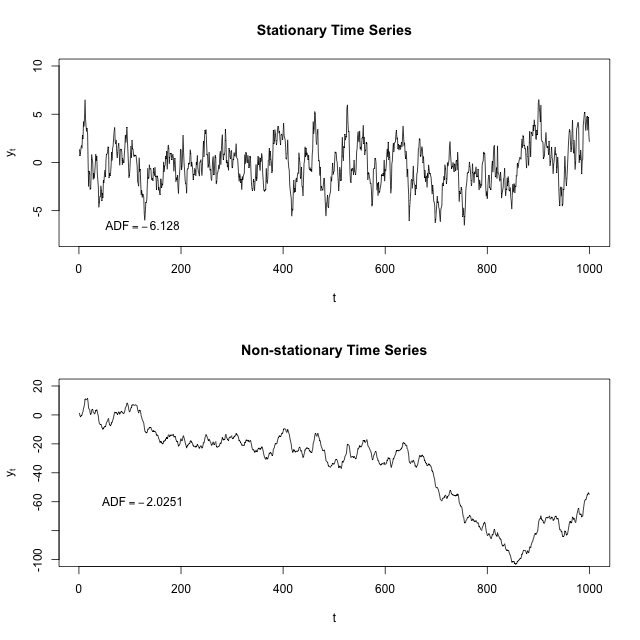
\includegraphics[width=0.8\textwidth]{Images/stationarycomparison.png} }
  \caption[Stationary and nonstationary time series comparison]{A comparison of stationary and nonstationary time series. (\cite{priestley1988})}
\label{fig:statnonstatcomp}
\end{figure}

\begin{dfn}[\cite{priestley1988}]
  A series $\{x_t\}_{t \in \ZZ}$ is called \textbf{stationary}, if $\{x_t\}_{t \in \ZZ}$ for any set of times $t_1, t_2, \dots, t_n$ and any $k \in \NN$, $P[x_{t_1}, x_{t_2}, \dots, x_{t_n}] = P[x_{t_1+k}, x_{t_2+k}, \dots, x_{t_n+k}]$, i.e. the joint probability distribution of $\{x_t\}_{t \in \ZZ}$ is not a function of time. It is called \textbf{nonstationary}, if it is not stationary.
\end{dfn}

The fundamental objective of time series analysis is to unveil the probability law which underlies the observed time series. A popular approach for doing this is to constrain the law to a class of the models, and then to find the most plausible model within this class. Two large distinct classes are linear and nonlinear models, and there are many different subclassifications of both. Historically, nonlinear models started to fully develop after it became apparent that some time series posses ``nonstandard'' (today called nonlinear) features, such as nonlinear relationship between expectations of temporally delayed variables, variation of predictability over state space and sensitivity to initial conditions (chaoticity).  These features are beyond the scope of standard linear models, such autoregressive (AR), moving average (MA) models and their derivations~\cite{fan2008nonlinear}, and time possessing them are called \textbf{nonlinear time series}.

% \begin{dfn}[\cite{bickel1996}]
%    A series $\{x_t\}_{t \in \ZZ}$ is called noisy chaotic \textbf{nonlinear}, if it satisfies the relation
%    \begin{align}
%      x_t = f(x_{t-1}) + \epsilon_t
%    \end{align}
%    for a general map $f : \RR \rightarrow \RR$ which is not linear, and where the noise component $\epsilon_t$ is i.i.d. and $E[\epsilon_t] = 0$. 
%    % When $f$ is a linear map, i.e.
%    % \begin{align*}
%    %   x_t = c x_{t-1} + \epsilon_t,
%    % \end{align*}
%    % then $\{x_t\}_{t \in \ZZ}$ is called \textbf{autoregressive} of order 1.
% \end{dfn}

\add[inline]{In a nonlinear system therefore, not only randomness, but also unmeasurable perturbations to the system can lead to apparent irregularity.}

EEG signals are known to be \emph{nonstationary and nonlinear}~\cite{kaplan2005, stam2005}. Moreover, they are prone to be infected with \emph{noise} due to imperfect isolation from the surrounding environment and patients involuntary movements, such as blinking or heartbeat. Since some patterns do not activate relative to a stimulus, a successful classifier must be able to detect a pattern regardless of its starting time, or find one. And finally, EEG records are relatively high dimensional - typical headsets containing 8-256 electrodes and sampling at 256 Hz result in 2048-65536 data points per second.

\section{Dynamical Systems} \label{sec:dynamical-systems}
\subsection{Definitions} \label{sec:dyn-sys-defs}

\begin{dfn}[\cite{andreas2000}]
  Assume that state of a system can be fully described by a finite set of $d$ variabes, such that each state corresponds to a point $\xi \in M$, where $M$ is a $d$-dimensional differentiable manifold. Then we will call $M$ a (true) \textbf{state space} or, equivalently, a (true) \textbf{phase space}, and $d$ its (true) \textbf{dimension}.
\end{dfn}

Although in this study, we will only consider Euclidean state space $M$, the true state space is needs not necessarily be Euclidean. For example, if some of the state variables are angles, the state space exhibits toroidal topology. However, any topological manifold is locally Euclidean~\cite{lee2010introduction} and, since, in EEG signal analysis both $M$ and $d$ are unknown, we have no other alternative than to work in Euclidean state space $M$.

\begin{dfn}[\cite{andreas2000}]
  Let $\mathbf{\xi} : \RR \rightarrow \RR^d$ be an $d \in \NN$ dimensional state (phase) space vector dependent on time, and $\mathbf{F}$ a smooth vector field in $\RR^d$. A \textbf{deterministic dynamical system}\footnote{In this work, we are going to assume that the brain is a deterministic dynamical system, and that any stochastic component is small and does not change nonlinear properties of the system. Thus, by the term dynamical system, we will always mean a deterministic dynamical system. This assumption is necessary for nonlinear dynamical analysis. On the other hand, nonlinear dynamical analysis also provides techniques (see Section~\ref{sec:surrogate-analysis-theory}) which can partially address (yet not fully answer) justification for this assumption. The question whether the brain is truly deterministic is open~\cite{stam2005, randomness}, but it is often thought to be probable that the brain is a nonlinear, deterministic, dissipative (i.e. exchanging energy with its environment) system~\cite{stam2005}.} is described by a set of $d$ first-order differential equations
  \begin{align*}
    \frac{d}{dt}\mathbf{\xi}(t) = \mathbf{F}(\mathbf{\xi}(t)), \qquad t \in \RR^+_0,
  \end{align*}
  such that there exists a unique\footnote{In other words, we assume that $\mathbf{F}$ satisfied the conditions of the uniqueness theorem of differential equations.} diffeomorphic\footnote{This means that $f^t$ is smooth, and has smooth inverse.} function $f^t : M \rightarrow M$ satisfying 
  \begin{align*}
    \mathbf{\xi}(t) = f^t(\mathbf{\xi}(0))
  \end{align*}
  for any initial condition $\mathbf{\xi}(0)$. We will call this mapping \textbf{state evolution function}, and vector field $\mathbf{F}$ \textbf{dynamics of the system}. We call the system linear if $\mathbf{F}$ is a linear vector field.
\end{dfn}

In late 1800s, H. Poincare\' developed a geometric approach to analyzing the stability (asymptotic evolution) of these systems via examination of the solution $(\xi_1(t), \xi_2(t), \dots, \xi_d(t))$ as a \emph{trajectory} in the phase space $M$ (assuming the solution is known, e.g. measured). These ideas were later extended into deeper understanding of chaos in dynamical systems~\cite{strogatz1996nonlinear}. 

In general, any system with temporally changing state is dynamic. A \emph{deterministic} dynamical system is describable by a model giving precise transition of a system from one state to another in time. This means that total description of system's evolution in its phase space (its \emph{trajectory}) is given by the initial state and a set of equations $\mathbf{F}$ (if $\mathbf{F}$ satisfies certain reasonable properties given by the uniqueness theorem). With \emph{stochastic} dynamical systems, such mapping is not possible, since these transitions are not given precisely.

A nonlinear dynamical system is a system where the differential equations describing its dynamics are nonlinear. Unlike in a linear system, changes in the initial state of a non-dynamical system are allowed to have a nonlinear relationship to the state space trajectory of the system~\cite{kaplan2005}.

It is important to note the obvious fact that in the case of EEG signal analysis, it is not possible to measure the true state of the system $\mathbf{\xi}(t)$. In fact, the observed variables are only a function of the true state of the system. To capture this, we will define a measurement function $s: \RR^d \subset M \rightarrow \RR^{d'}, \, d' \ll d$, as
\begin{align*} \label{eq:meas-fun}
  s(\mathbf{\xi}(t)) = \mathbf{x}(t) + \mathbf{\eta}(t),
\end{align*}
where $\mathbf{\eta}(t)$ is measurement noise, which encompasses the measurement error and the noise coming from the measurement conditions. In the following text, we will usually disregard the measurement function and assume we have direct access to $\mathbf{\xi}(t)$ and thus assuming the observed state equals the true state $\mathbf{x}(t) \equiv \mathbf{\xi}(t)$, since is usually neglected in the explained theory. Nevertheless, it is important to remember that the noise term have affect the results we obtain using the theory explained theory. % We will return to this issue in Section~\ref{sec:embedding}.

% $s(\xi(t))$ for some (generally noninvertible) measurement function $s: \RR^d \rightarrow \RR^{d'}$, where $d' \ll d$. Morover, the time between subsequent measurements is limited by a sampling frequency and the values of the variables themselves are taken and stored with a limited precision.

\subsection{Attractor} \label{sec:attractor}
Depending on the properties of $\mathbf{F}$, there are several possibilities of how the system might evolve when as $t \rightarrow \infty$. In the following, we will focus on so called dissipative dynamical systems (of which brain is considered a member~\cite{stam2005}).
\begin{dfn}[\cite{kantz2004}]
  A dynamical system is called dissipative, when it is the case that
  \begin{align}
    E[|\det \mathbf{J}_{\mathbf{F}}|] < 1,
  \end{align}
  where $\mathbf{J}_{\mathbf{F}}$ is the Jacobian of vector field $\mathbf{F}$ and the expectation is taken over the state space $M$. In other words, average state space volume of a set of initial conditions of non-zero measure is contracted as the system evolves. 
\end{dfn}

For these systems, after sufficient passage of time, all future states will continue evolving on a bounded, time-invariant subset of $M$. This subset is a geometrical object called an \textbf{attractor}. Example of four basic attractors, point, limit, torus and chaotic attractors, can be seen in Figure~\ref{fig:attractors}. Examples of several chaotic attractors are shown in Figure~\ref{fig:attractor-examples}~\cite{strogatz1996nonlinear, grassberger1983measuring, mackey1977oscillation}.

\begin{figure} 
\centering
\noindent\makebox[\textwidth]{%
  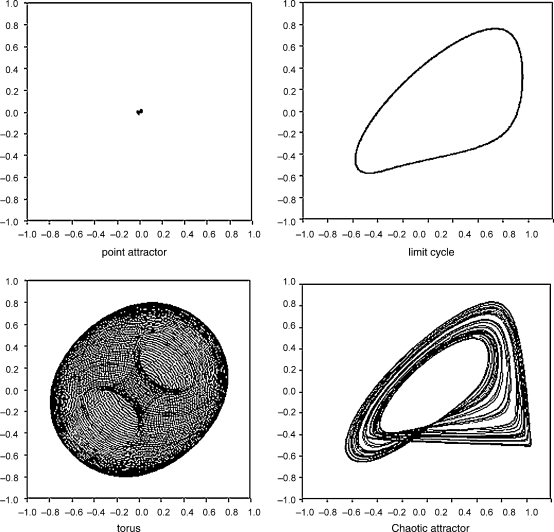
\includegraphics[width=0.8\textwidth]{Images/attractors.png} }
  \caption[Illustration of attractor types.]{Visualization of four common attractor types (units are arbitrary). Left to right, top to bottom:
    \textbf{Point attractor} is the only type of attractor of linear deterministic dissipative systems. It consist of a single final state to which all points from the corresponding region of attraction evolve to.
    \textbf{Limit cycle} corresponds to a periodic dynamical system. It is formed by set of states visited periodically, consituting a trajectory through the state space.
    \textbf{Torus attractor} corresponds to a quasi-periodic dynamical system, resulting (in this example) from a superposition of two periodic oscillations.
    \textbf{Chaotic} (strange) \textbf{attractor}, characteristic of dynamical systems with extending (instead of shrinking) volumes in \emph{some} directions. Corresponding dynamical system may appear stochastic, yet still be completely deterministic~\cite{andreas2000}. (\cite{stam2005})}
\label{fig:attractors}
\end{figure}

\begin{figure} 
\centering
\noindent\makebox[\textwidth]{%
  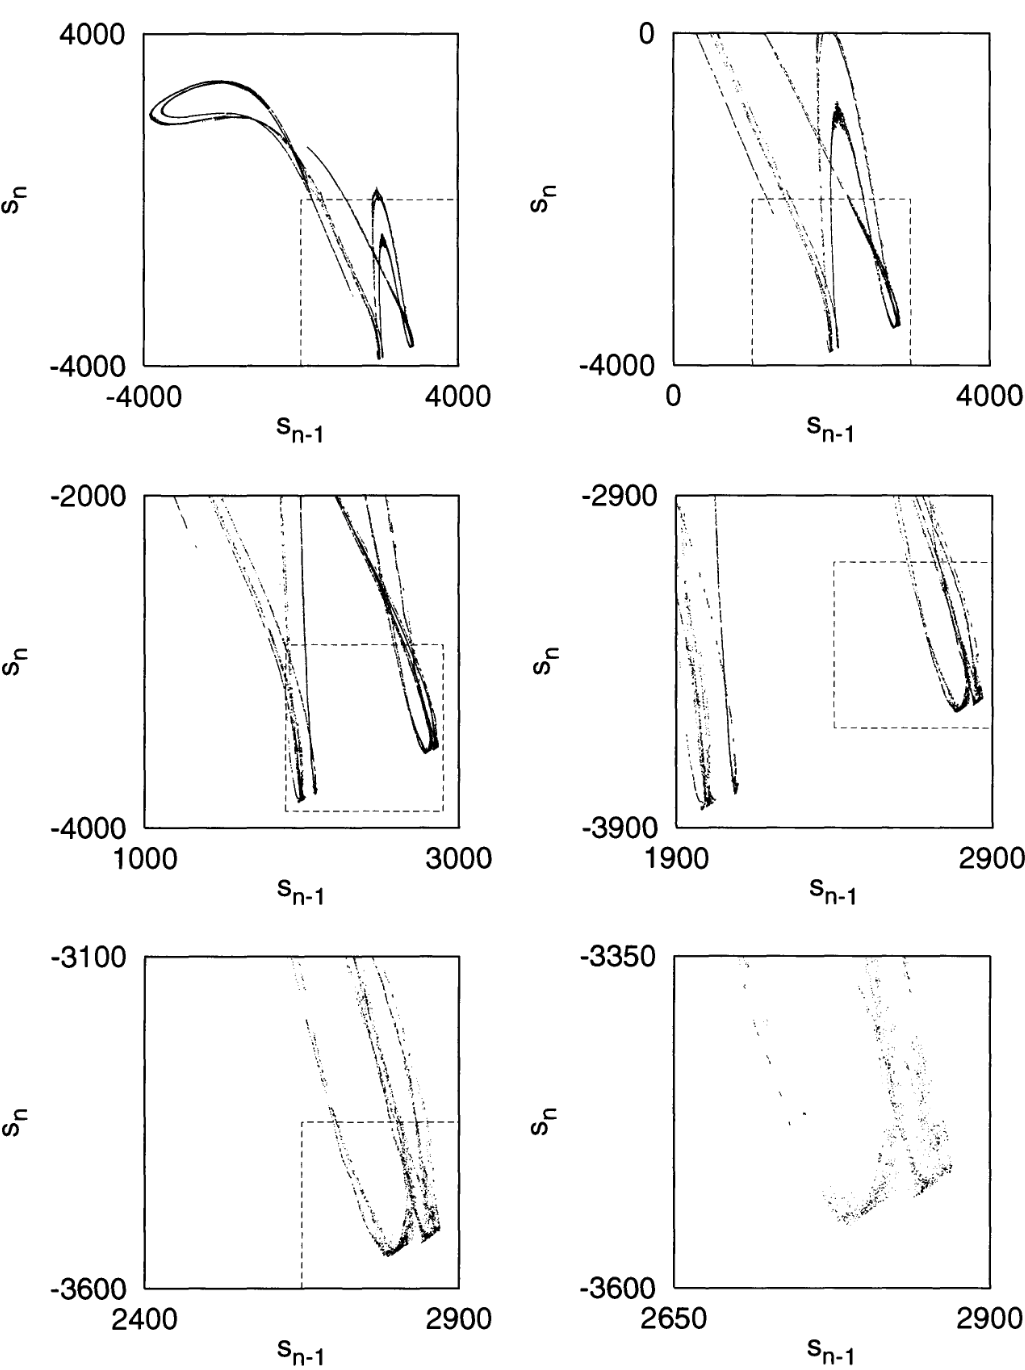
\includegraphics[width=0.8\textwidth]{Images/self-similarity.png}}
  \caption[Illustration of self-similarity.]{Noise-reduced visualization of successive enlargements of highly self-similar attractor~\cite{kantz2004}.}
\label{fig:self-similarity}
\end{figure}

\begin{figure} 
\centering
\noindent\makebox[\textwidth]{%
  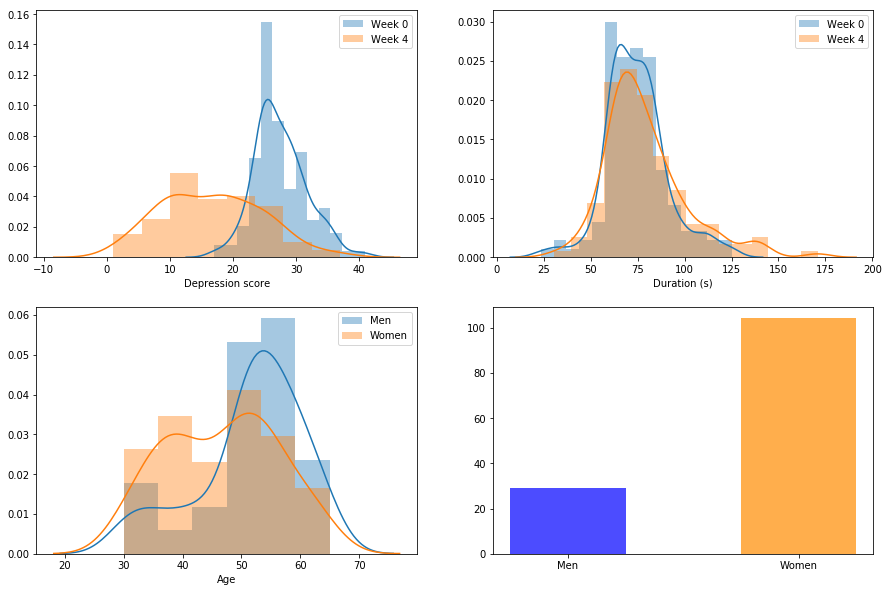
\includegraphics[width=1.0\textwidth]{./Images/dataset.png} }
  \caption[Attractor examples.]{Lorenz, Roessler and Mackey-Glass attractors generated from corresponding systems of differential equations~\cite{strogatz1996nonlinear}. These systems are known to exhibit chaotic dynamics for certain parameter values~\cite{grassberger1983measuring}.}
\label{fig:attractor-examples}
\end{figure}

Statistical methods can be used to analyze observations of a complex system. Another branch of mathematics providing us with powerful tools to study systems with apparently complex behavior is chaos theory, which studies so called chaotic systems. These systems exhibit dynamics which extend volumes of clusters of initially nearby states in some directions. Although there is mixed evidence on low dimensional chaos in the brain and in the biological systems in general, its techniques have found many successful applications in their analysis~\cite{skinner1994low}. 

Attractors of chaotic systems, coined by Ruelle and Takens in 1971 \emph{chaotic} (strange) \emph{attractors}~\cite{ruelle1971nature}, possess interesting properties. Since, as mentioned, attractors are bounded, the divergence of nearby states due to chaos eventually stops and the two trajectories fold together~\cite{kantz2004}. This continuous expansion and folding creates a ``self-similar'', \emph{fractal} object. An example of a strange attractor can be seen in Figure~\ref{fig:self-similarity}.

This self-similarity can be quantified by a class of scalar measures called \emph{fractal dimensions}. Indeed, we will use one of the members of this class - correlation dimension - in our experiments, and will treat it in detail. In addition, let us give another example of a fractal dimension, called box-counting dimension, be useful for understanding the implications of Taken's embedding theorem (\ref{thm:takens}) in Section~\ref{sec:embedding}:
% Since many physiogenerated signals are chaotic, their analysis is concerned primarily with \emph{chaotic} (strange) \emph{attractors}. These attractors are relatively complex, characteristic of dynamical systems with extending volumes in some directions. This property results fast divergence of two initial states, one of which has nonzero component in the direction of growth, i.e. sensitive dependence on the initial conditions. However, since atractors are bounded, the divergence eventually stops and the two trajectories fold together. This continuous expansion and folding may create an attractor with a \emph{fractal structure}, which, for our purposes, can be understood to mean ``possessing a quantifiable self-similarity'' (an example of such an attractor is shown in Figure~\ref{fig:self-similarity})~\cite{andreas2000}. 
\begin{dfn}[\cite{falconer2004}] \label{def:box-counting}
  Let $F$ be any non-empty bounded subset of $\RR^n$, and let $N_\epsilon(F)$ be the smallest number of sets of diameter at most $\epsilon$ (``mesh cubes'') which can cover $F$. Then, the \textbf{box-counting dimension} (also known as Minkowski–Bouligand dimension) is defined as
  \begin{align} \label{eq:box-counting}
    d_0(F) = \lim_{\epsilon \rightarrow 0} -\frac{\log N_\epsilon(F)}{\log{\epsilon}} \, ,
  \end{align}
  if it exists.
\end{dfn}
Intuitively, the number of mesh cubes of side $\epsilon$ intersecting $F$ gives an indication about how irregular the set is when inspected at scale $\epsilon$, and the box-counting dimension reflects ``how rapidly'' the irregularities develop as $\epsilon \rightarrow 0$~\cite{falconer2004}. 

\subsection{Stationarity} \label{sec:stationarity}
Nonstationarity is a phenomenon which considerably complicates practical analysis of dynamical systems. All the techniques presented in this text assume stationary process, since this assumption is a prerequisite to deterministic chaos~\cite{isliker1993test}. We will call system \textbf{nonstationary} if the dynamics of the system are influenced by causes lying outside of them (and \textbf{stationary} if the opposity is true). In ergodic theory (study of the invariant measures of dynamical systems), the concept of stationarity is defined more rigorously. However, these definitions are not suited for numerical applications~\cite{andreas2000}. Nevertheless, a relevant subset of nonstationary systems can be defined more explicitly:
\begin{dfn}[\cite{andreas2000}]
  A dynamical system is called \textbf{nonautonomous} if its dynamics $\mathbf{F}$ are explicitly dependent on time:
  \begin{align*}
    \frac{d}{dt}\xi(t) = \mathbf{F}(\xi(t), t), \qquad t \in \RR^+_0.
  \end{align*}
\end{dfn}

No reliable tests for nonstationarity in this strong sense exist. There is another common definition of a stationary process (sometimes referred to as weak stationarity). A process is called \textbf{weakly stationary}, if all statistical second-order quantities (like mean, variance, and power spectrum) are independent of the absolute time, and at most function of relative times~\cite{isliker1993test}.

This weaker definition employs only linear quantities, and is therefore not strictly suitable for nonlinear time series analysis. On the other hand, statistical tests of this property exist. In our study, we use the following test for weak stationarity discussed by H. Isliker and J. Kurths in~\cite{isliker1993test}.

This technique attempts to approximate a projection of so called \emph{physical invariant measure} $\rho$ defined in~\cite{eckmann1985ergodic} as the time average of Dirac $\delta$-distributions along a trajectory:
\begin{align*}
  \rho(\mathbf{\xi}) \coloneqq \lim_{T \rightarrow \infty} \frac{1}{T} \int_0^T \delta_{\mathbf{\xi}(t)} \diff t \, .
\end{align*}
Roughly speaking, this measure quantifies ``how often'' are different subsets of the state space visited over infinite time. In other words, it gives a probability that a randomly chosen point on a trajectory will happen to belong to a given subset ``after enough time passed''. It is a statistical description of a system in the state space which contains information about all statistical moments~\cite{isliker1993test}, which should be indepent of the trajectory length for a stationary process.

%Since this measure is ergodic\footnote{This means, roughly, that it is not decomposable into several different pieces, each again invariant~\cite{eckmann1985ergodic}.}, the ergodic theorem basically states that the space and time averages using ergodic measures are equal almost everywhere, which in the case of measure $\rho$ translates to
%\begin{align*}
%   \int_{\mathrm{state space}} f(\xi) \rho(\diff \xi) = \lim_{T \rightarrow \infty} \frac{1}{T} \int_0^T f(\xi(t)) \diff t
% \end{align*}
% for any $f \in C$ defined on the state space $M$. 

\info[inline]{This measure is related to computation of correlation dimension. Mention it in corresponding section.}

Let $x_1$ represent the time series of the measured quantity, and $N$ be the length of the time series. The algorithm then computes the projection $\rho(x_1)$ as follows. The range of the time series is divided into $K$ ``equiprobable'' intervals $[ x_1^{(k)}, x_1^{(k+1)} ]$, $k=1, 2, \dots, K$, such that the interval boundaries are K-quantiles of the distribution of the values of the time series (i.e. application of the quantile function of the distribution to the values $1/K, 2/K, \dots, (K-1)/K$), and the number of values falling into each of those intervals is counted:
\begin{align*}
  n_k &\coloneqq \# \{ x_1^{(k)} \leq x_1 \leq x_1^{(k+1)} \} \\
  &\approx \sum_{x_1} \int_{x_1^{(k)}}^{x_1^{(k+1)}} \delta(x-x_1) \diff x \\
  &= \sum_{x_1} \chi_{[x_1^{(k)}, x_1^{(k+1)}]}(x_1),
\end{align*}
where $\chi_{[a,b]}$ is the characteristic function of the set $[a,b]$. The density over the entire series is then approximated by a histogram with $K$ bins as
\begin{align*}
  p_k^{\mathrm{all}} = \frac{n_k^{\mathrm{all}}}{\sum_k n_k^{\mathrm{all}}}.
\end{align*}

If the system is stationary, then the probability distribution for the first half of the time series should be the same as for the entire time series. Hence, this distribution (with the same intervals) is computed for the first half of the time series ($n_k^{\mathrm{half}}$). Then, the two probability distributions are compared using the $\chi^2$ statistical test with the null hypothesis of stationarity. The corresponding Pearson's cumulative test statistic then is
\begin{align*}
  \chi^2 \coloneqq \sum_k \frac{(n_k^{\mathrm{half}} - Zp_k^{\mathrm{all}})^2}{Zp_k^{\mathrm{all}}},
\end{align*}
where $Z = \ceil{N/2} = \sum_k n_k^{\mathrm{half}}$. Under the null hypthesis, this quantity is expected to have $\chi^2$ distribution~\cite{isliker1993test}, and thus the Pearson's test can be used to potentially reject the hypothesis of stationarity of the observed time series.

\subsection{Recurrence Plot} \label{sec:recplot}
When presented with the task of finding regularities in measurements obtained from nonlinear dynamical systems, one possible approach is analysing at least approximate repetitions of simple patterns, which can be further used for reconstruction of more complicated rules. Recurrence plot, proposed by Eckmann in~\cite{eckmann1987}, is a method of visualizing obtained state-space trajectory segments in relation to each other in order to achieve this goal. Furthermore, it can be used to test necessary conditions for validity of dynamical parameters derivable from a nonlinear time series such as the correlation dimension, entropies and Lyapunov exponents~\cite{manuca1996stationarity}. The property which makes them especially interesting is that the information contained in recurrence plots is not easily obtainable by other known methods~\cite{eckmann1987}.

\begin{dfn}[\cite{eckmann1987}]
  Let $N$ be the length of given time series, $\mathbf{x}_i$ for $i \in \{1,2,\dots,N \}$ be a $i$-th delay vector of any integer embedding dimension, $\norm{\cdot}$ a norm, $\Theta(\cdot)$ a Heaviside step function, and $\epsilon \in \RR_0^+$ a tolerance parameter. Then, \textbf{recurrence plot} is the matrix
  \begin{align}
    M_{ij} = \Theta(\epsilon - \norm{ \textbf{x}_i - \textbf{x}_j }) \, .
  \end{align}
\end{dfn}

In other words, $M_{ij}$ is a symmetric\footnote{Although this is true for our definition, it may not be true for an alternative definition using a more general topology instead of a norm. For example, each point may have been assigned its own $\epsilon$-neighborhood.} binary $N \times N$ matrix, where $M_{ij} = 1$ when $i$-th and $j$-th points of the reconstructed trajectory enter each other's $\epsilon$ neighborhood. Since those points are, in fact, times, recurrence plots are a way of visualizing subtle time correlation information.

In~\cite{eckmann1987}, J. Eckmann et al. analyzed patterns typically observed in recurrence plots and distinguished between large-scale \emph{typology} and small-scale \emph{texture}. Moreover, they were able identify multiple different patterns easily distinguishible by the human eye typical of dynamical systems with distinct properties. This work was furhter extended in~\cite{marwan2007recurrence}.

The essential drawback of recurrence plot is their size - it is quadratic in the length of the time series. A simple way of reducing its dimension is to partition the time series into disjoined segments, and let $M_{ij}$ represent the distance between those two segments. This technique, introduced in~\cite{manuca1996stationarity}, is known as \textbf{meta-recurrence plot}. The measure for ``dynamical closeness'' between two segments is based on the correlation integral (\ref{eq:corrsum}) we will introduce in Section~\ref{sec:corrdim}.

A more objective approach to analyzing recurrence plots is an ensemble of techniques group under the term Recurrence Quantification Analysis (RQA). Using these techniques, a number of scalar measures can be used to quantify properties of recurrence plots, such as determinism, periodicity, chaos and stationarity~\cite{marwan2011avoid}. An important ingredient for computation of these measures is the distribution of lengths of diagonal lines in the plot. It can be shown that this distribution is directly related to correlation dimension, which we will cover in Section~\ref{sec:corrdim}~\cite{marwan2007recurrence}.

\section{State Space Reconstruction} \label{sec:state-space-reconstruction}
In the previous section, we have introduced a concept of state space of a dynamical system. In the case of EEG analysis, however, our observations do not directly form a state space object, but a set of time series', one for each electrode. Moreover, it is necessary to deal with the fact that our data, however rich, rarely represent complete information about the studied system. In the case of EEG signals, the complete state of the system at any moment is determined by many variables, and the sensors are only able to collect traces of their cumulative effects (and noise). So we are confronted with a problem: how to convert this data into state space trajectories? This procedure is called \emph{state space reconstruction}.

However, it is not necessary to reconstruct the entire original state state space of the system. In general, we are only interested in the subspace where the attractor of the system evolves. Thus, one possible approach to nonlinear time series analysis consists of the following steps~\cite{stam2005}: 
\begin{enumerate}
  \item reconstruction of the attractor \info{Saying dynamics is not true. We are not reconstructing the vector field $\mathbf{F}$.} of given system from recorded data,
  \item characterization of the reconstructed attractor,
  \item checking validity of the results with surrogate data testing.
\end{enumerate}

\subsection{Embedding} \label{sec:embedding}
To the goal of state space reconstruction, let $\mathbf{x}_n$ be the reconstructed vector we are trying to find, and let us have a time series $x$ of scalar measurements $x_1, x_2, \dots, x_N$ of a quantity dependent on the current state of the system. As mentioned in Section~\ref{sec:dyn-sys-defs}, we will discard the noise term $\eta_n$ in (\ref{eq:meas-fun}) and assume that the observed value corresponds to the true value.\footnote{For theoretical implications of the noise term one may consult~\cite{kugiumtzis1996state}.} Furthermore, let us consider a function $\Phi: \RR^d \subset M \rightarrow \RR^{m}$, such that $\mathbf{x}_n = \Phi(\xi(n \Delta t))$. Such function is called an \textbf{embedding}, and $m \in \NN$ is called the embedding dimension. What properties does $\Phi$ have to satisfy so that it provides useful information about the true state space trajectories?

Firstly, note that we assume the studied dynamical system to be deterministic. If our reconstructed embedded space is to represent the true state space, evolution of any state on every trajectory we observe in the embedded space should depend only on its current state. Therefore, we may reasonably require $\Phi$ to be one-to-one, i.e. contain no intersections~\cite{fraser1989reconstructing}. This will be relevant in Sections~\ref{sec:delay} and~\ref{sec:ild}.

Secondly, since many of the attractor properties we care about (such as correlation dimensions, Lyapunov exponents, etc.) are only invariant under smooth non-singular transformations~\cite{fraser1989reconstructing}, in order to preserve these properties in the embedded space, we require $\Phi$ to preserve the differential structure of the state space $M$ (which corresponds to the tangent map $\mathrm{grad} \Phi$, which is a $m \times d$ matrix constant for every $\mathbf{\xi}$) also being a one-to-one mapping~\cite{andreas2000}. The proof of Taken's Theorem~\ref{thm:takens} mentioned later also requires this property. 

These two properties together are equivalent of $\Phi$ being a diffeomorphism, and form necessary and sufficient conditions for $\Phi$ being and embedding~\cite{andreas2000} between the state space $M$ and the embedding space $\Phi(M)$. The dynamical system $\mathbf{F}$ on $M$ then induces unique dynamical sytem on $\Phi(M)$~\cite{andreas2000}.

As we have stated in Section~\ref{sec:dynamical-systems}, our observations are formed by application of noninvertible measurement function $s: \RR^d \rightarrow \RR^{d'}$, $d' \ll d$, to the true states of the system. Aside from being a projection, $s$ may be also be a distortion. With those properties of $s$, it might seem impossible to reconstruct the true state space trajectory and this indeed may be the case in some situations. On the other hand, there are quantities invariant under distortion which may be preserved~\cite{andreas2000}. Moreover, if our goal was to study only the attractor properties, perfect reconstruction may not even be desirable in the case that the attractor dimension is smaller than the dimension of the original space~\cite{kantz2004}.

\subsection{Method of Time Delays} \label{sec:method-of-delays}
There are two approaches to the problem of state space reconstruction for EEG time series data:
\begin{description}
  \item [Time delay embedding] state space is reconstructed separately for each time series.
  \item [Spatial embedding] each electrode represents a dimension of the embedding space, and each vector in the reconstruction contains amplitudes measured at a particular time.
\end{description}

It has been demonstated, however, that spatial embedding, when applied to EEG, does not reliably reconstruct the complexity of state space dynamics. Instead, in this case, is rather a measure of cross-correlation between individual channels~\cite{pritchard1996validity}. It seems to remain relatively obscure approach to embedding, being used in a minority of groups.\footnote{Which, however, strongly advocate for its use ~\cite{pezard1999bother, lachaux1997spatial, kantz1997scalar}.} On the other hand, time delay embedding is widely used, and, as we will show in this section, has a long history and relatively strong theoretical basis.


It had been already known since 1936, that every $n$-dimensional differentiable manifold can be embedded in $\RR^{2n+1}$, and that the set of such embeddings is open and dense in the space of generic smooth maps, which is known as Whitney's theorem~\cite{whitney1936}.\footnote{The second part of the theorem is a consequence of the fact that two hyperplanes with dimensions $d_1$ and $d_2$ in $m$-dimensional space are likely to intersect if $d_1 + d_2 \geq m$.} In other words, $2n+1$ independent measurements of a $n$-dimensional system can be uniquely mapped to a $2n+1$ dimensional space, hence each such $2n+1$ dimensional vector identifies identifies state of the system perfecly, thus reconstructing the true state space.

Time delay embedding is a technique of state space reconstruction, which achieves the same goal, but with a single measured quantity. It was first introduced into the field of nonlinear dynamical system analysis by N. H. Packard in 1980 (although it was already being used in different fields in 1950s~\cite{andreas2000}). Studying the Rossler system, Packard noticed that by sampling a single coordinate, he was able to obtain a faithful phase-space representation of the original system by simply using a value of a coordinate with its values at two previous times~\cite{packard1980}. In other he demonstrated numerically that past and future measurements of one variable contain information about the unobserved variables and can be used to define the present state.

In particular, for each time $t$, we define an embedding window $\tau_w$, and use measurements obtained at times $t'$ for $t \leq t' \leq t + \tau_w$. To this goal, we use $m$ measurements, $\tau$ elements apart. Here, $\tau$ is called \emph{lag} or \emph{time delay}, and is measured in number of samples.\footnote{Some authors use the time units $\tau \Delta t$, where $\Delta t = t_s = 1/f_s$ is the sampling period.} Using the notation in the Section~\ref{sec:embedding}, the time delay reconstruction is then formed by the following vectors
\begin{align}
  \textbf{x}_n = (x_n, x_{n+\tau}, x_{n+2\tau}, \ldots, x_{n+(m-2)\tau}, x_{n+(m-1)\tau}) \, ,
\end{align}
for $n > (m-1)\tau = \tau_w$~\cite{kantz2004}. 

A year after Packard's discovery, in~\cite{takens1981}, F. Takens has proved theoretically that the attractor reconstructed using this method may have the same dynamical properties (entropy, dimension, Lyapunov spectrum) as attractor of the original system under some conditions. Takens delay embedding theorem is an important result of nonlinear time series analysis and can be stated as follows:
\begin{thm}[\cite{takens1981}] \label{thm:takens}
  Let $M$ be a compact\footnote{This theorem can be proved for $M$ non-compact provided less restrictions are imposed on $s$.} smooth manifold specifying the state space of a deterministic dynamical system of dimension $d \in \NN$, $s : M \rightarrow \RR^n, s \in C^2$ a smooth measurement function, $f^t : M \rightarrow M, f \in C^2$ a set smooth diffeomorphic state evolution functions for $t \in \RR$. Then the set of maps $\phi_{(s,f^t)} : M \rightarrow \RR^{2d+1}$, defined by
  \begin{align}
    \phi_{(s,f^t)}(x) = (s(\xi), s(f^{-\tau}(\xi)), \dots, s(f^{-2d\tau}(\xi))),
  \end{align}
  for which $\Phi$ is an embedding is an open and dense set in the space of maps satisfying the assumptions above.
\end{thm}

This idea has a simile in the existence theorems in the theory of differential equations, which say that a unique solution exists for each $x(t), \dot{x}(t), \ddot{x}(t), \dots$. For example, in many body dynamics under Newtonian gravitation, knowledge of a body's position and momentum is sufficient to uniquely determine its future dynamics~\cite{ScholarpediaReconstruction}.

Taken's theorem, although of theoretical importance, is not necessarily useful in practice, since even dense sets can have measure zero. Moreover, it is restricted to smooth manifolds. An add came ten years later, when T. Sauer both generalized Takens' result as follows (in a simplified form):
\begin{thm}[Sauer,~\cite{sauer1991}] \label{thm:sauer}
  Let $A$ be a compact fractal with box-counting dimension $d_A$ (see Definition~\ref{def:box-counting}), and let $A$ be a subset of a $m$-dimensional manifold. Then a member of the set
  \begin{align*}
    \lbrace \Phi: A \rightarrow \RR^{m} | \Phi \in C^1, m > 2d_A \rbrace \text{ is an embedding with probability } 1.
  \end{align*}
\end{thm}

Theorem~\ref{thm:takens} and Theorem~\ref{thm:sauer} together ensure that when $m$ is chosen such that $m > d_A$ (which may be a considerable reduction in dimension compared to $m \geq 2d+1$), then $\Phi$ a true embedding of the underlying attractor for almost any $\tau$ (note only sufficiency of the result - $\textbf{x}_n$ may be an embedding even for smaller $m$).

A fascinating consequence of Theorem~\ref{thm:sauer} when applied to a sequence of measurements recorded from a physical system is that a successfully reconstructed attractor does not describe the time series, but the system itself. In the words of Theiler: ``If one believes that the brain (say) is a deterministic system, then it may be possible to study the brain by looking at the electrical output of a single neuron. This example is an ambitious one, but the point is that the delay-time embedding makes it possible for one to analyze the self-organizing behavior of a complex dynamical system without knowing the full state at any given time''~\cite{theiler1990estimating}.

\subsection{The Effects of Noise}
Although these theoretical results are important to know about, they all make practically unrealistic assumptions, such as infinite amount of data and infinite measurement precision, and absence of noise. Moreover, practical applications present further challanges, such as presence of noise. Several factors complicate successful reconstruction from real-world, experimental data~\cite{casdagli1991state}:
\begin{description}
  \item[Observational noise.] Given a reconstructed vector $\mathbf{x} \in \RR^m$, there is a (approximatly Gaussian shaped in natural scenarios) distribution $p(\mathbf{x})$ in the reconstruction space due to the noise term in equation (\ref{eq:meas-fun})~\cite{andreas2000}.
  \item[Dynamic noise (nonstationarity).] External influences perturb the system, which consequently appears nondeterministic.
  \item[Estimation error.] Estimation of the dynamics of the system is performed using only limited amount of data.
  \item[Quantization error.] The measured analogue quantity is converted and stored as a number with only finite number of bits.
\end{description}

Moreover, different reconstructions can amplify the already present noise to varying degree. In~\cite{casdagli1991state}, Casdagli et al. provide a quantitative way of analyzing this amplification, and, by extension, of insight into selection of embedding parameters so that the noise amplification is minimized.

\subsection{Time Delay Selection} \label{sec:delay}
Note that the results of theorems in Section~\ref{sec:method-of-delays} do not depend on the value of the delay $\tau$.\footnote{This is because of the fact that the measurements are infinitely precise~\cite{casdagli1991state}.}. Embeddings with the same value of the embedding dimension $m$, but different values of $\tau$ are theoretically equivalent. In practice, however, some theoretically sound time delay reconstructions may fail to be embeddings. Although some researchers propose that the only important parameter is the length of the embedding window $\tau_w = \tau (m-1)$~\cite{kugiumtzis1996state}, as we will see, the choice of time delay has effects independent of the choice of embedding dimension, and vice versa. Some of the reasons a reconstruction may fail to be an embedding are as follows:
\begin{enumerate}
  \item The embedding may fail to be a one-to-one map due to finite precision, or presence of noise in the data~\cite{andreas2000}.
  \item For some highly chaotic systems with large Lyapunov exponents (see Section~\ref{sec:lyap}) and large dimension, projection to a low dimensional time series causes amplifies the effects noise. As a result, this imposes limits on short term predictablity and state space reconstruction may become impossible. Such systems should be treated as operationally stochastic~\cite{casdagli1991state}.
  \item It was shown that increasing $\tau$ leads to rise in entropy~\cite{Kantz1997}.
  \item Deterministic behavior can be observed only when $\tau_w$ is smaller than the time scale of the foldings naturally produced as result of time embedding~\cite{casdagli1991state}.
  \item If the values of $\tau$ are \emph{too small} in comparison to the typical time scales of the series (measured e.g. by mean period), then the successive elements of reconstructed state space vectors become almost equal. This effect is often called \emph{redundance}. Since $x_t \approx x_{t + \tau}$, the reconstructed attractor will concentrate along the main diagonal (see Figure~\ref{fig:delay}, left hand side). Moreover, in this case, the effect of noise is amplified~\cite{casdagli1991state}.
  \item If the values of $\tau$ are \emph{too large}, the successive elements in the reconstructed vector are almost independent. This effect, called \emph{irrelevance} or \emph{overfolding} is even magnified if the underlying attractor is chaotic, since deterministic correlations between states are lost even at very small time scales, i.e. even measurements performed at time $t$ and $t + \tau$ for very small $\tau$ may be already unrelated. The reconstructed attractor will form a seemingly random clound in $\RR^m$ - thus the reconstructed attractor may appear complex, even if the true attractor is simple (see Figure~\ref{fig:delay}, right hand side). 
\end{enumerate}

In summary, picking the proper value of $\tau$ is a balancing act between redundance and irrelevance. It is important to minimize excessive foldings, and extreme closeness between adjacent points on the trajectory (ideally, the distances between points is same in the reconstructed as in the true space).

\begin{figure} 
\centering
\noindent\makebox[\textwidth]{%
  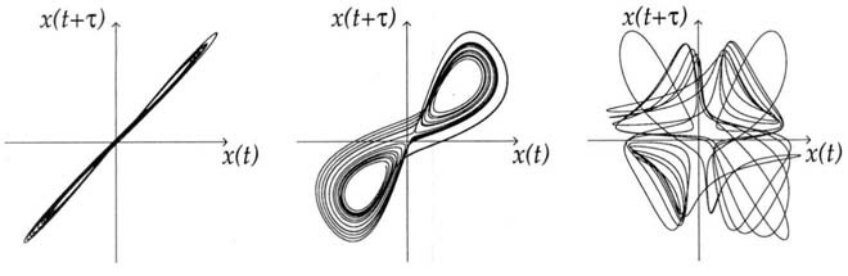
\includegraphics[width=1\textwidth]{Images/delay.png} }
  \caption[Effects of time-delay on reconstruction.]{Time delay reconstructions of the Lorenz attractor for different values of $\tau$. Figure on the left hand side shows choice of small $\tau$ and represents the case of redundance - the states concentrate along the main diagonal. Figure in the middle shows a successful reconstruction (although not an embedding, for which $m \geq 3$ is required). Figure on the right hand side shows a choice of large $\tau$ and represents the case of irrelevance - the reconstruction lacks apparent structure~\cite{andreas2000}.}
\label{fig:delay}
\end{figure}
\subsubsection{Autocorrelation} \label{sec:acorr}
From the above, we understand that each of a successful reconstruction should provide valuable information about the state of the system. This may mean ``reasonably'' low statistical correlation between values of coordinates of the reconstructed vectors $\mathbf{x}_n$. Thus, a natural method of estimating the optimal time delay is studying the \emph{autocorrelation function} $A$, and picking the first $\tau$ where $A(\tau)$ decays below a threshold value - commonly used are $A(0)/e$~\cite{stam2005}, $1-A(0)/e$~\cite{kantz2004}, or even the first local minimum~\cite{albano1993reliability, abarbanel2012analysis} or the first $0$ crossing~\cite{kantz2004}.

\begin{dfn}[\cite{kantz2004}]
  Let $x$ be a scalar time series of measurements $x_1, x_2, \cdots, x_N$. \textbf{Autocorrelation} $A : \NN \rightarrow \RR$ for time delay $\tau$ is given by
  \begin{align*}
    % A(\tau) = \frac{1}{\mathrm{var}} \langle (s_n - \langle s_n \rangle )(s_{n-\tau} - \langle s_n \rangle) \rangle \\
    % A(\tau) = \frac{E[(x_i - \overline{x})(x_{i-\tau} - \overline{x})]}{\mathrm{var}}, 
    A(\tau) = \frac{1}{\mathrm{var} (N-\tau)}\sum_{i=1}^{N-\tau}(x_i - \overline{x})(x_{i+\tau}+\overline{x})
  \end{align*}
  where $\overline{x}$ is the mean of the time series, and $\mathrm{var}$ is its variance.
\end{dfn}

Note that $\mathrm{var}$ normalizes autocorrelation function to $A(0) = 1$. White noise produced $A(\tau) = 0$ for all $\tau \neq 0$. Filtered noise and chaotic time series can be expected to have $A(\tau)$ slowly decaying to zero with increasing time delay~\cite{andreas2000}.

Computing the autocorrelation function is not only useful for examining the stationarity of the time series, but it also gives a geometrical insight into the shape of the attractor: if we approximate the cloud of reconstructed vectors $\mathbf{x}_n \in \RR^m$ by an ellipsoid, lengths of its semi-axis are given by the square root of the eigenvalues of its auto-covariance matrix. In two dimensions, zero of the covariance matrix corresponds to those eigenvalues being equal, i.e. $x_t$ and $x_{t+\tau}$ being completely uncorrelated~\cite{kantz2004}. An obvious objection is that correlation between $x_t$ and $x_{t+\tau}$ says nothing about correlation between $x_t$ and $x_{t+2\tau}$, etc. Indeed, this method computes correlations only between two successive coordinates, but since it neglects possible correlations between other pairs of coordinates, it is mostly useful for low dimensional systems~\cite{krakovska2015use}.

Autocorrelation also provides a lower bound for $\tau$ in the following sense. If the data is noisy, vectors formed by time delay embedding procedure are practically meaningless, if the variation of the signal in the time covered in the time window $\tau_w = (m-1)\tau$ is less than the variation of noise. This means that $\tau$ should be selected such that $A(\tau) > A(0) - \mathrm{var}_{\text{noise}}/\mathrm{var}_{\text{signal}}$~\cite{kantz2004}. Of course, in practice, it may be difficult to estimate variance of noise in the data.

\subsubsection{Delayed Mutual Information} \label{sec:dmi}
Another commonly used method is to use the first minimum of the \emph{time delayed mutual information}~\cite{fraser1986independent}. 

\begin{dfn}[\cite{kantz2004}]
  Let probability density of the values of a time series be split into $\epsilon$-wide histogram bins. Let $p_i$ be the probability that a signal assumes value in $i$-th bin of the histogram, and let $p_{ij}(\tau)$ be the the probability that $x_t$ is in a bin $i$ and $x_{t+\tau}$ is in a bin $j$. \textbf{Delayed mutual information} $\mathcal{I}_{\epsilon}$ for time delay $\tau$ is defined as
  \begin{align*}
    \mathcal{I}_{\epsilon}(\tau) = \sum_{i, j} p_{ij}(\tau) \ln p_{ij}(\tau) - 2 \sum_{i} p_i \ln p_i.
  \end{align*}
\end{dfn}

In other words, time delayed mutual information is the average mutual information between measurements obtained by the original time series and its $\tau$-shifted (time delayed) counterpart. The optimal $\tau$ is usually selected as $\argmin_{\tau} \mathcal{I}_{\epsilon}(\tau)$.

Although this approach yields coordinates independent in a more general sense than simple linear independence provided by the autocorrelation function, the same criticism applies: minimum dependence between $x_t$ and $x_{t-\tau}$ says nothing about dependencies between other coordinates. Again, using this method is justifiable only for two-dimensional reconstructions. However, delayed mutual information has been generalized for multiple dimensions by its proponent A. M. Fraser using multidimensional distributions into a concept he called \emph{redundancy}, which basically measures the degree to which the reconstructed vectors accumulate around the bisectrix of the embedding space~\cite{fraser1989reconstructing}. Another criticism of delayed mutual information that some systems exhibit slowly decaying mutual information which has no minima~\cite{martinerie1992mutual}. 

\subsubsection{Average Displacement from Diagonal} \label{sec:adfd}
\textbf{Average displacement from diagonal} is a simple technique which simply measures the average distance of the embedding vectors from their original location:
\begin{align*}
  \mathrm{ADFD}(m, \tau) = \frac{1}{N_{(m, \tau)}}\sum_{i=1}^{N_{(m, \tau)}} \norm{ \mathbf{x}_i^{(m, \tau)} - \mathbf{x}_i^{(m, 0)}},
\end{align*}
where $\mathbf{x}_i^{(m, \tau)}$ is the $i$-th vector of time delay embedding with embedding dimension $m$ and time delay $\tau$.

Rosenstein et al. presented multiple methods for quantifying expansion from the diagonal (the identity line of the attractor), and found $\mathrm{ADFD}$ to be the most computationally efficient, robust to noise, and accurate~\cite{rosenstein1994reconstruction}. They also experimentily identified optimal $\tau$ as the one for which the slope of $\mathrm{ADFD}$ drops below 40\% of its initial value.  

\subsubsection{Singular Values Analysis} \label{sec:svd}
All the approaches described so far address the issue of redundance by attempting to make the coordinates less correlated or expanding the reconstruction from the identity line. The issue of irrelevance however, needs to be addressed as well. In fact, based mostly on empirical, rather than theoretical grounds, most time delay estimation techniques optimize for the following criteria~\cite{kugiumtzis1996state}:
\begin{enumerate}
  \item The reconstructed attractor must be expanded from the diagonal.
  \item The components of the reconstructed vector $\mathbf{x}_n$ must be uncorrelated.
\end{enumerate}
Those criteria are similar, and bias towards larger estimates of $\tau$. This leads many authors to suggest more advanced techniques, such as generalized delayed mutual information mentioned above, or some of those introduced in the following text.

Principal component analysis, in particular, can be used to measure the volume occupied by the reconstructed attractor. Both overfolded and redundant attractors may be marked by low volume~\cite{andreas2000}.

Given a fixed embedding dimension $m$, the corresponding $m$ singular values as a function of $\tau$ contain information about the degree of extension of the embedded vectors in the $m$ directions in the reconstructed space. Rapid increase followed by rapid decrease of some singular values accompanied by the opposite behavior of others indicate a collapse of the attractor. Also, high number of large singular values is an indicator of volume of the reconstructed attractor.

If we assume, without loss of generality\unsure{Is this so?}, that the time series is standardized and denote
\begin{align*}
  \mathbb{X} \coloneqq \begin{pmatrix} \mathbf{x}_1^T \\ \mathbf{x}_2^T  \\ \dots \\ \mathbf{x}_{N_{(m, \tau)}}^T  \end{pmatrix},
\end{align*}
then
\begin{align*}
  (\mathbb{C})_{ij} \coloneqq (\mathbb{X}^T\mathbb{X})_{ij} = A\left( (i-j)\tau \right).
\end{align*}
This matrix is symmetric and thus diagonalizable, and also at least non-negative definite. Its eigenvalues are called the singular values, and correspond the the magnitude of variance of projections of the embedded vectors into individual directions of the principal components.

If the time delay is too small, then all the elements of matrix $\mathbb{C}$ will have similar value $(\mathbb{C})_{ij} \approx A(0)$, and thus there will be one dominant singular value, while others will remain close to zero. This singular value then corresponds to the main diagonal of the attractor.

If the time delay is too large, then the diagonal elements will approach average of the squared time series $(\mathbb{C})_{ii} \approx \langle x^2 \rangle$, while the remaining elements will converge to zero due to decay of the autocorrelation function, $\mathbb{C} \approx c\mathbb{I}$ for some constant $c$. This corresponds to the reconstruction forming a featureless noise~\cite{andreas2000}.

One drawback of this method is that it requires evaluation either by a human or a more complicated algorithm. Moreover, it was suggested that although this method is effective noise reduction technique, its effectiveness at delay estimation is less clear - the number of large singular values is sensitive to noise~\cite{mees1987singular}.

\subsubsection{Integral Local Deformation} \label{sec:ild}
In Section~\ref{sec:dyn-sys-defs}, we require our dynamical systems to be deterministic, which means that no trajectories in the state space should intersect themselves. Moreover, in real physical systems, it may be reasonable to assume that it is highly unlikely to find closeby trajectories of opposite or orthogonal directions. This property is maintained by a successful embedding, and (if the assumption holds) can occur only in an improper reconstruction.

T. Buzug and G. Pfister presented a quantitative measure of these close trajectory intersections by comparing the the evolutions of reference trajectories with centroids of points on the neighboring trajectories~\cite{buzug1992optimal}. For the optimal embedding, divergence between these trajectories should be minimized.

First, multiple random reference points are chosen. Let $\mathbf{x}_i(0)$ be such a reference point at time 0. Then, either a fixed number of nearest neighbors or all neighbors within a given radius and their centroid $\mathbf{x}_i^{\mathrm{COM}}(0)$ (where COM stands for ``center of mass'') are found. Then, the absolute growth of the distance between the centroid of those originally neighboring points and the reference point after $qt_{ev}$ time steps is found as:
\begin{align*}
  \Delta(q,m,\tau) = \norm{\mathbf{x}^{\mathrm{COM}}(qt_{ev}) - \mathbf{x}_i(qt_{ev})} - \norm{\mathbf{x}_i^{\mathrm{COM}}(0) - \mathbf{x}_i(0)}.
\end{align*}

The values $\Delta(q,m,\tau)$ are discretely integrated from $q=1$ to $q=q_{max}$:
\begin{align*}
  \mathcal{D}(m, \tau, i) = \frac{t_{ev}}{2} \sum_{q=1}^{q_{max}} \left( \Delta(q-1,m,\tau) - \Delta(q,m,\tau) \right).
\end{align*}
This expression, called \textbf{integral local deformation}, is then averaged over $N_{ref}$ reference points and normalized:
\begin{align*}
  \mathrm{ILD}(m, \tau) = \langle \mathcal{D}(m, \tau, i) \rangle_i = \displaystyle{ \frac{t_{ev} \displaystyle{ \sum_{i=1}^{N_{ref}} } \displaystyle{ \sum_{q=1}^{q_{max}} } \left( \Delta(q-1,m,\tau) - \Delta(q,m,\tau) \right)}{2N_{ref} \Delta t \left( \max_{i \in 1, 2, \dots, N} x_i - \min_{i \in 1, 2, \dots, N} x_i \right)} }
\end{align*}

Finally, we obtained a measure of non-homogeneity of the average flow in the neighborhood of the points in the reconstructed embedding space as a function $\mathrm{ILD}_m(\tau)$ of the time delay $\tau$ and parameterized by $m$. According to our assumption about the reasonable property of physical dynamical systems, the optimal $\tau$ for each $m$ is the minimum $\argmin_{\tau} \mathrm{ILD}_m(\tau)$.

The ILD algorithm provides the detailed information about the flow of the reconstruction, and is arguably the most powerful out of the algorithms we described, since it is the only one which measures the \emph{dynamical} properties of the reconstruction, not only topological ones~\cite{andreas2000}. Moreover, since we may expect that for a sufficiently high $m$, the $\mathrm{ILD}_m(\tau)$ curves will converge~\cite{buzug1992optimal}, this technique allows for simultaneous estimation of both the embedding dimension $m$ and the time delay $\tau$. However, one considerable drawback is much larger computational cost, since for each $m$ and $\tau$, closest neighbors from the entire reconstruction have to be determined for each point.

\subsection{Embedding Dimension Selection}
\subsubsection{False Nearest Neighbors} \label{sec:fnn}
Since the dynamics $\textbf{F}$ are assumed to be a \emph{smooth} vector field and the attractor $A$ is a \emph{compact} set in the phase space, its members acquire near neighbors, which should be subject to similar evolution. Therefore, these neighbors should remain close to each other after a short interval of time (even though chaos may introduce exponential divergence between them). This is a useful fact, which can be used, for example, to predict future evolution of a trajectory, or a computation of Lyapunov exponents. The \textbf{false nearest neighbors} algorithm uses them for estimation of embedding dimension~\cite{kennel1992determining}.

The main idea is to use the transition from dimension $m$ to dimension $m+1$ in the embedding procedure to differentiate between ``true'' and ``false'' neighbors. If the embedding dimension $m$ is too small, some members of $A$ that are close to each other may not be neighbors in the true state space, simply because the true state space is projected down to a smaller space\add{Add the figure from Kennel.}. These members are \emph{false neighbors}, all other neighbors are \emph{true}. When the attractor is fully unfolded into large enough dimension and is properly embedded, all neighbors are true.

Let $n(j,r,m,m)$ denote the index of of $r$-th nearest neighbor of the $m$ dimensional embedding vector $\mathbf{x}_j$. Then, let $R_m(j,r,m)$ denote the Euclidean distance between $\mathbf{x}_j$ and its neighbor:
\begin{align*}
  R_m(j,r,m) = \norm { \mathbf{x}_j - \mathbf{x}_{n(j,r,m)} }_2 = \sqrt{ \sum_{k=0}^{m-1}[ x_{j+k\tau} - x_{n(j,r,m)+k\tau} ]^2 }
\end{align*}

Then, any near neigbor for which the distance increase after transition from dimension $m$ to dimension $m+1$ is large in comparison to the initial distance is marked as false:
\begin{align} \label{eq:first-criterion}
  \left[ \frac{R_m^2(j,r,m) - R_{m+1}^2(j,r,m)}{R_m^2(j,r,m)} \right]^{1/2} = \frac{ x_{j+k\tau} - x_{n(j,r,m)+k\tau} }{R_m(j,r,m)} > R,
\end{align}
where $R \in \RR$ is some threashold. The $m$ for which the relative proportion of false neighbors to all neighbors reaches zero is the embedding dimension suggested by this criterion.

This criterion, by itself, is not sufficient for determining proper embedding dimension. When applied to limited amount of white noise data, it erroneously suggested embedding the noise into a low dimensional attractor. This happens because even though a state may be a nearest neigbor, it is not necessarily temporally close, and thus the assumptions above do not hold. The experiments performed by Kennel et al. show for such states it is usually $R_m(j,r,m) \approx R_A$, where $R_A$ is radius of the attractor. Furthermore, for increasing amount of data, the embedding dimension suggested by this criterion also increased - behavior not observed for relatively small dimensional attractors~\cite{kennel1992determining}. 

Therefore, Kennel et al. propose another criterion in addition to the one above. Since false neighbors which are near, but temporally distant, are usually stretched to the extremeties of the attractor with transition from $m$ to $m+1$, they suggest marking all near neighbors satisfying
\begin{align} \label{eq:second-criterion}
  \frac{R_{m+1}(j,r,m)}{R_A} > A
\end{align}
as false, where $R_A$ may be computed as, for example 
\begin{align*}
  R_A = \frac{1}{N} \sum_{j=1}^{N} \left[ x_j - \overline{x} \right]^2.
\end{align*}

Although this technique is commonly used, it is not without its drawbacks. An obvious point is that altough it is true that distance between neighbors in unfolded attractor should not grow with increase in dimension, the inverse is not necessarily true, i.e. stable distance between near neighbors with increase in dimension does not guarantee that these neighbors are true. 

The authors suggest some values of the tolerance parameters they found useful in their experiments, but, in general, the results of this technique may depend on the choice of $R$ and $A$. Their selection is subjective and somewhat arbitrary. The best course of action is to evaluate the technique for multiple values of $R$ and $A$ and select those with the most ``reasonable'' results.

In practice, it has been found that the results of this method are sensitive not only to the tolerance parameters $R$ and $A$, but also to the lag as well~\cite{kugiumtzis1996state}. 

Also, this method tends to underestimate $m$ for very small $\tau$. Small $\tau$ forces the attractor to lie near the diagonal in $\RR^m$ and further increasing $m$ imposes very little effect on the geometry of the attractor. In effect, most points will appear as true neighbors leading to a wrong conclusion~\cite{kugiumtzis1996state}.

Lastly, in presence of measurement noise, the proportion of false neighbors may increase after transition to a higher dimension, since even identical vectors will diverge~\cite{kantz2004}.

\subsubsection{Average False Neighbors} \label{sec:afn}
This technique by Cao~\cite{Cao1997} addresses one of the drawbacks of false nearest neighbors mentioned in the previous section - the variance of results based on subjective choice of embedding parameters. It does so by defining two parameter free functions dependent only on the embedding parameters.

The first function measures the variation of average ratio of distance of two neighbors in one dimension to the distance of the same neighbors in a higher dimension. More precisely, let
\begin{align*}
  E(m) =\frac{1}{N_{(m, \tau)}} \sum_{i=1}^{N_{(m,\tau)}} \frac{ \norm {\mathbf{x}_i^{(m+1)} - \mathbf{x}_{n(i,1,m)}^{(m+1)} }_{\infty} }{ \norm{ \mathbf{x}_i^{(m)} - \mathbf{x}_{n(i,1,m)}^{(m)} }_{\infty} },
\end{align*}
where $n(i,1,m)$ denotes the nearest neighbor of vector $\mathbf{x}_i$ in dimension $m$, and $\norm{ \cdot }_{\infty}$ denotes the Chebyshev norm\footnote{This norm is suggested by the author, but another norm can be used.}. Then, the first statistic is defined as
\begin{align*}
  E_1(m) = \frac{E(m+1)}{E(m)}.
\end{align*}
In principle, $E_1(m)$ saturates and stops increasing after some threshold $m$ for systems with finite embedding dimension. 

For systems with infinite embedding dimensions it may be difficult in practice to resolve whether $E_1$ indeed stopped increasing or is still slowly increasing. Alternatively, it may still saturate because of limited amount of data. For this reason, Cao introduces another statistic, whose purpose is to distinguish stochastic from deterministic sources of data.

Let
\begin{align*}
  E^*(m) = \frac{1}{N - m\tau} \sum_{i=1}^{N - m\tau} | x_{i + m\tau} - x_{n(i,1,m) + m\tau} |.
\end{align*}
Then, similarly to above, the second statistic is defined as
\begin{align*}
  E_2(m) = \frac{E^*(m+1)}{E^*(m)}.
\end{align*}

Since, for random time series, the future values are independent of the present ones, the ratio $E_2(m)$ is expected to be close to 1 for all $m$.

\section{Nonlinear Measures} \label{sec:nonlin-meas}
In this section, we will study quantities invariant under embedding. These can be further use to characterize the dynamics of deterministic dynamical systems.
\subsection{Lyapunov Exponents} \label{sec:lyap}
The characteristic property of chaotic systems is their sensitivity to initial conditions - similar causes need not have similar effects. Consequently, even small uncertainty in the current state of the system (due to, at best, with limited storage space) results in virtual impossibility of predicting future state of the sytem more than a short amount of time into the future, since uncertainty in the initial state is expanded at exponential rate with passage of time by the chaotic dynamics for the predicted future states. % (see Figure ).

Lyapunov exponents can be used to quantify this sensitivity~\cite{kantz2004}. Consider a small sphere of initial conditions $B_r(\mathbf{x})$ for a state $\mathbf{x}$ in the phase space, $r$ infinitesimal, and $\mathbf{x}_n \in B_r(\mathbf{x})$. To study the evolution of states in this ball,  we can use a linear approximation of $\mathbf{F}$. Let us assume that $\mathbf{x}_{n+1} = \mathbf{F}(\mathbf{x}_n)$. Then for infinitesimal divergences $\delta \mathbf{x}_n$, $\delta \mathbf{x}_{n+1}$, we have
\begin{align*}
  \delta \mathbf{x}_{n+1} = T^{(n)} \delta \mathbf{x}_n,
\end{align*}
for a tangent map $T^{(n)}$ defined as
\begin{align*}
  (T^{(n)})_{ik} = \frac{\partial F_i(\mathbf{x}_n)}{\partial x_{n+k}}.
\end{align*}

Product of these tangent maps for subsequent states along a trajectory can be written as a product of two rotations and a diagonal matrix~\cite{grassberger1991nonlinear}:
\begin{align*}
  \prod_{n=1}^{N} T^{(n)} = R_d T_{diag} R_b,
\end{align*}
where $(T_{diag})_{ij} = (T)_{ij}$ for $i=j$ and $(T_{diag})_{ij} = 0$ for $i \neq j$. 

Then, the Lyapunov exponents can be defined as~\cite{grassberger1991nonlinear}
\begin{align*}
  \lambda_i = \lim_{n \rightarrow \infty} \frac{1}{N} \log (T_{diag})_{ii}.
\end{align*}

In other words, as the system evolves, $B_r(\mathbf{x})$ expands (or contracts) exponentially in $m$ directions defining semiaxes of a sphere, where length of each semiaxis corresponds to the rate of expansion (or contraction) in the corresponding direction. The average lengths of these semiaxis for $\mathbf{x}$ over the entire state space are exactly Lyapunov exponents. Hence, $m$ dimensional system has exactly $m$ Lyapunov exponents, collectively called its \emph{Lyapunov spectrum}.

Computation of the Lyapunov spectrum for analyticial given $\mathbf{F}$ is straightforward using the definition above. But for dynamics given implicitly in a time series is difficult (although some algorithms, e.g. the one introduced by Eckmann in 1986~\cite{eckmann1986liapunov}). It is commonly agreed that estimating Lyapunov exponents is even more difficult than esimating correlation dimension~\cite{andreas2000}, although they have been successfully employed in EEG analysis~\cite{roschke1995nonlinearschizo, roschke1995nonlineardeppression, hosseinifard2013, stam2005}. It has been claimed by P. Grassberger et al. that any application of these measures to physical systems should be interpreted with caution, mainly because all physical measurements are corrupted by noise, and reliable separation of signal is not always possible~\cite{grassberger1991nonlinear}. They suggest that when emplying these techniques, the goal should not be to estabilish to strongest form of determinism, but to use them to ask whether determinism can be ruled out at all.

Since the direction of the largest Lyapunov exponent dominates growth, we can say that the average rate of separation between two points in the phase space with similar initial conditions can be characterized by the largest Lyapunov exponent. As a consequence, it is unnecessary to compute the entire Lyapunov spectrum - which would require identifying appropriate Lyapunov directions - if our goal is to find a global property of the system characterizing the degree of average instability and unpredictability. It is sufficient to measure the average rate of separation~\cite{Rosenstein1993}. 

Hence, let us define $\norm {\mathbf{s}_{n_1} - \mathbf{s}_{n_2}} = d(0) \ll 1$ as an initial distance between two nearby points in the state space, and $d(i) = \norm { \mathbf{s}_{n_1 + i} - \mathbf{s}_{n_2 + i}}$. Then, the largest Lyapunov exponent $\lambda_1$ can be approximated as
\begin{align} \label{eq:lyap}
  d(i) = d(0) e^{\lambda_1 (i \Delta t)}, \quad d(i) \ll 1, \quad i \rightarrow \infty, \quad d(0) \rightarrow 0,
\end{align}
where $\Delta t$ is sampling time of the time series.  

The Lyapunov exponents carry the units of an inverse time - $1/\lambda_1$ gives a typical time scale for the divergence or convergence of nearby trajectories~\cite{kantz2004}. Equivalently, $1/\lambda_1$ is (on average) an upper bound on predictability in the system~\cite{andreas2000}. Also equivalently, they also can be seen as quantification of the degree of chaos in the system; a sigle positive exponents is a sufficient indication of presence of chaos~\cite{Rosenstein1993}.

\add[inline]{Say what different values of $\lambda_1$ say about the system.}

\subsubsection{Rosenstein's algorithm} \label{sec:rosenstein}
In the following, we will describe \emph{Rosenstein's algorithm} for computation of the largest Lyapunov exponent~\cite{Rosenstein1993}. This algorithm was found to be relatively robust to noise, values of the embedding parameters and limited amount of data.

First, state space is reconstructed using time delay embedding (see Section~\ref{sec:embedding}). The suggested method of time delay selection is the autocorrelation method (see Section~\ref{sec:acorr}).

For given embedding dimension $m$ and each point on the trajectory $\mathbf{x}_j$, the algorithm locates the nearest neighbor $\mathbf{x}_{n(j,m)}$, such that their distance in the embedded space is minimized:
\begin{align*}
  d_j(0) = \norm { \mathbf{x}_j - \mathbf{x}_{ n(j,m) } }.
\end{align*}

As an approximation, we want to assume $\mathbf{x}_j$ and $\mathbf{x}_{n(j,m)}$ to be nearby initial conditions, but at the same time, we know they lie on the same trajectory. Hence, we may impose a condition on their minimal temporal separation, called a \emph{Theiler window}. In the original paper~\cite{Rosenstein1993}, Rosenstein suggests
\begin{align*}
  \frac{1}{4} \text{ time series length} > \left| j - n(j,m) \right| > \text{mean period of the time series}.
\end{align*}

Then, assuming the $j$-th pair of nearest neighbors diverge exponentially at a rate given by the largest Lyapunov exponent, we have
\begin{align*}
  d_j(i) \approx d_j(0) e^{\lambda_1(i \Delta t)}.
\end{align*}

By taking logarithm of both sides, we obtain

\begin{align*}
  \ln d_j(i) \approx \ln d_j(0) + \lambda_1 (i \Delta t).
\end{align*}

This represents a set of lines, one for each point on the reconstructed trajectory, each with a slope roughly proportional to $\lambda_1$. So, the algorithm approximates the largest Lyapunov exponent by least squares fit to the average line
\begin{align*}
  d(i) = \frac{1}{\Delta t} \langle \ln d_j(i) \rangle_{j = 1, 2, \dots, N_{(m, \tau)}},
\end{align*}
usually evaluated for values $i \in \langle 0, t_e \rangle$, where $t_e$ is called the evolution time.

Note that the user may decide to set $\Delta t = 1$ and work with units of time series indeces instead of seconds. It is well known that the results of the largest Lyapunov exponent may vary drastically based on input parameters~\cite{fell1994resonance}. Moreover, we can even rescale or shift the data, since Lyapunov exponents are invariant under any smooth invertible map.

There are many other algorithms to compute the larest Lyapunov exponents, such as Kantz's algorithm~\cite{kantz1994robust}, Eckmann's algorithm~\cite{eckmann1986liapunov}, Wolf's algorithm~\cite{wolf1985determining} (relatively unstable, it is impossible to distinguish exponential divergence~\cite{kantz2004}), and Sato's algorithm (produces spurius results in certain cases~\cite{Rosenstein1993}). The main competetive advantage of Rosenstein's algorithm is its easy implementation, low computational cost, and robustness to noise (due to averaging in the last step) and applicability to small datasets~\cite{Rosenstein1993}.

\info[inline]{As we have mentioned already, the projection involved in the measurement may make distances shrink apparently for short times, although they grow in the true state space~\cite{kantz2004}. Moreover, in the true state space distances do not grow everywhere on the attractor with the same rate, and locally they may even shrink. LLE is average of those local divergence rates. Influence of noise can be minimised by using an appropriate averaging statistics.}

\subsubsection{Dataset Size Requirements} \label{sec:req-lyap}
The minimum dataset requirements was estimated by Eckmann and Ruelle in~\cite{eckmann1992fundamental} by imposing requirements on the distances and number of neighbors for each point. If $\Gamma(r) \gg 1$ is the average number of neighbors withing radius $r$, we may approximate it as
\begin{align*}
  \Gamma(r) \approx \mathrm{const.} \times r^m,
\end{align*}
and we also know that $\Gamma(d) \approx N$, where $d$ is the diameter of the attractor. Therefore, we obtain
\begin{align*}
  \Gamma(r) \approx N \left( \frac{r}{d} \right)^m \gg 1 \implies N > \left( \frac{d}{r} \right)^m.
\end{align*}
For example, if we require the ratio of the average distance to the nearest neighbor to the extent of the attractor to be $r/d \leq 0.1$, we have $N > 10^m$ as the minimum time series length requirement.

\subsection{Correlation Dimension} \label{sec:corrdim}
\begin{figure} 
\centering
\noindent\makebox[\textwidth]{%
  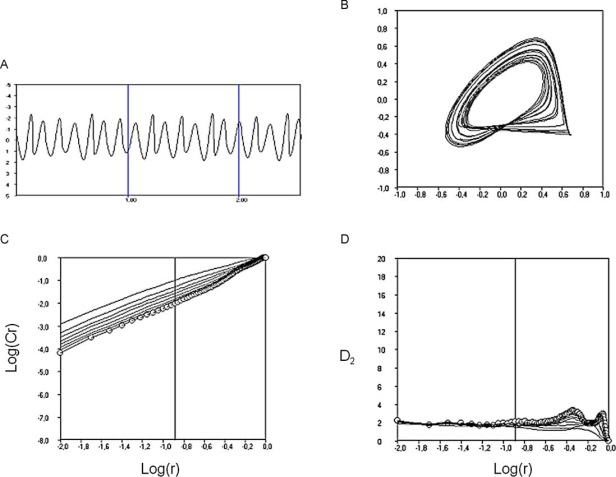
\includegraphics[width=0.8\textwidth]{Images/corrdim.png} }
  \caption[Example of $D_2$ computation.]{Example computation of the correlation dimension~\cite{stam2005}. The axes are dimensionless. In the clockwise direction starting from the upper left hand side, the figures show the original time series, the reconstructed attractor, logarithmic plot of the correlation integrals $C(r)$ for different values of the embedding dimension $m$ (starting with $m=2$ in the uppermost line, and increasing by one with each line below), and their derivatives, corresponding to the correlation dimension $D_2$. In the derivatives plot, the vertical line signifies the cutoff of $\log r$ after which the values become imprecise due to numerical instability. We can see that the derivatives converge to approximately $2$ with decreasing radius $r$.}
\label{fig:corrdim}
\end{figure}

The world of mathematics offers numerous definitions of dimension (box-counting dimension (\ref{eq:box-counting}), Hausdorff dimension, information dimension, etc.) and similar quantities, but many of them can be regarded as variations of the following, simple and intuitive analogy:~\cite{theiler1990estimating}
\begin{align} \label{eq:dim-intuitive}
  \text{bulk} \approx \text{size}^{\text{dimension}} \implies \text{dimension} = \lim_{\text{size} \rightarrow 0} \frac{\log \text{bulk}}{\log \text{size}}.
\end{align}
In other words, dimension can be loosely defined as scaling of ``bulk'' (corresponds to mathematical concept of measure) as a function of its linear ``size''. Of course, dimensions of different definitions may not be equal to each other, but for our purposes, we are interested in the most computationally accessible.

Unlike Lyapunov exponents, which measure dynamical properties of the system, (correlation) dimension is a purely geometrical property of the attractor, independent of the ordering of the reconstructed vectors. \unsure{Is this true?}

In this thesis, we are interested in dimension estimation for the following reasons:
\begin{enumerate}
  \item Even a system with high number of degrees of freedom, such as a brain, may actually evolve in a much lower-dimensional subspace. The number of active degrees of freedom may provide a measure of complexity of the observed system. This information is available in the attractor of the system and it can be shown that this property is preserved by state space reconstruction~\cite{andreas2000}.
  \item It can help distinguish stochastic and deterministic processes, since stochastic processes, after sufficient passage of time, use all available state space dimensions.
\end{enumerate}
Of course, although these expectations can be justified theoretically, the numerical reality may be different.

Most definitions of dimension are based on first covering the studied object in the state space with the smallest possible balls (using a given metric). Correlation dimension is a special case of generalized box-counting dimension (which is a generalization of box-counting dimension already introduced in Definition~\ref{def:box-counting}), defined as
\begin{align*}
  D_{\kappa}(A) = \lim_{r \rightarrow 0} \frac{1}{\kappa} \frac{ \log \int_M (\mu(B_r(\mathbf{x})))^{\kappa} \diff \mu( \mathbf{x})}{ \log r},
\end{align*}
where the integration is over the whole state space $M$ and $\mu$ is measure concentrated on $A$.
If we define $\mu$ as
\begin{align} \label{eq:measure}
  \mu(\mathbf{x}) \coloneqq \int_M \Phi (r - \norm{\mathbf{x} -\mathbf{y}}) \diff \mu (\mathbf{y})
\end{align}

The we can write the, ``bulk'' of $A$, so called generalized correlation integral as
\begin{align*}
C(\kappa, r) = (\int_M \left( \mu(B_r(\mathbf{x})))^{\kappa} \right)^{\frac{1}{\kappa}} = \left[ \int_M \left(\int_M \Phi (r - \norm{\mathbf{x} -\mathbf{y}}) \diff \mu (\mathbf{y})) \right)^{\kappa} \diff \mu (\mathbf{x}) \right]^{\frac{1}{\kappa}} 
\end{align*}
It can indeed be shown that $C(\kappa, r) \propto r^d_{\kappa}$.

In the continuous case, correlation dimension than takes to form
\begin{align*}
  D_2(A) = \lim_{r \rightarrow 0} \frac{\log C(r,2)}{\log r}.
\end{align*}

As explained in Section~\ref{sec:recplot}, correlation dimension is closely related to the distribution of lengths of diagonal lines on recurrence plots. Intuitively, we can see that both methods are measuring temporal correlations in the original time series.

\subsubsection{Grassberger-Procaccia Algorithm}
There are essentially three ways of computing correlation dimension: box-counting algorithms, pairwise distance algorithms, and nearest neighbors algorithms. Grassberger-Procaccia algorithm, which we use to compute correlation dimension, is a variant of a pairwise distance algorithm.

This class of algorithms, used in discrete cases with limited amount of data, estimates the measure of a box centered on point $\mathbf{x}_i$ in the reconstructed space as
\begin{align*}
  \mu_i = \frac{1}{N_{(m,\tau)}}
\end{align*}
and zero everywhere else.

Thus, in the discrete case, the correlation sum $C(r)$ can be computed as 
\begin{align} \label{eq:corrsum}
  C(r) \coloneqq C(r,2) = \frac{2}{N_{(m,\tau)}(N_{(m,\tau)}-1)} \sum_{i<j} \Phi(r-\norm{\textbf{x}_i - \textbf{x}_j}).
\end{align}
which corresponds to the fraction of pairs of points in the phase space whose distance is smaller than $r$. Under certain reasonable conditions, correlation sum is an unbiased estimator of the correlation integral~\cite{ScholarpediaGpa}. In our application, we also use a lower bound on the distance of pairs of points, which is called a Theiler window, noted $w_t$.

Typical behavior of the correlation sum is shown in Figure~\ref{fig:exp-cr}. We can see that the curves are forced to meet at the same point for all $m$ - for high enough $r$, all points are counted and $C(r)=1$ (or $C(r) = \binom{N_{(m,\tau)}}{2}$ not normalized). As the lines shift to the right with increasing $m$ and stay parallel in the proper scaling region, the slope near that point necessarily increases with $m$. For high enough $m$, the scaling region disappears. Moreover, the values of $C(r)$ are inaccurate for small $r$ due to noise and for small $C(r)$ due to statistical fluctuations (corresponding to horizontal lines). Thus, there is only a limited interval of $r$ and limited set of embedding dimensions $m$ for which an accurate estimation of $D_2$ can be made~\cite{andreas2000}.

\begin{figure} 
\centering
\noindent\makebox[\textwidth]{%
  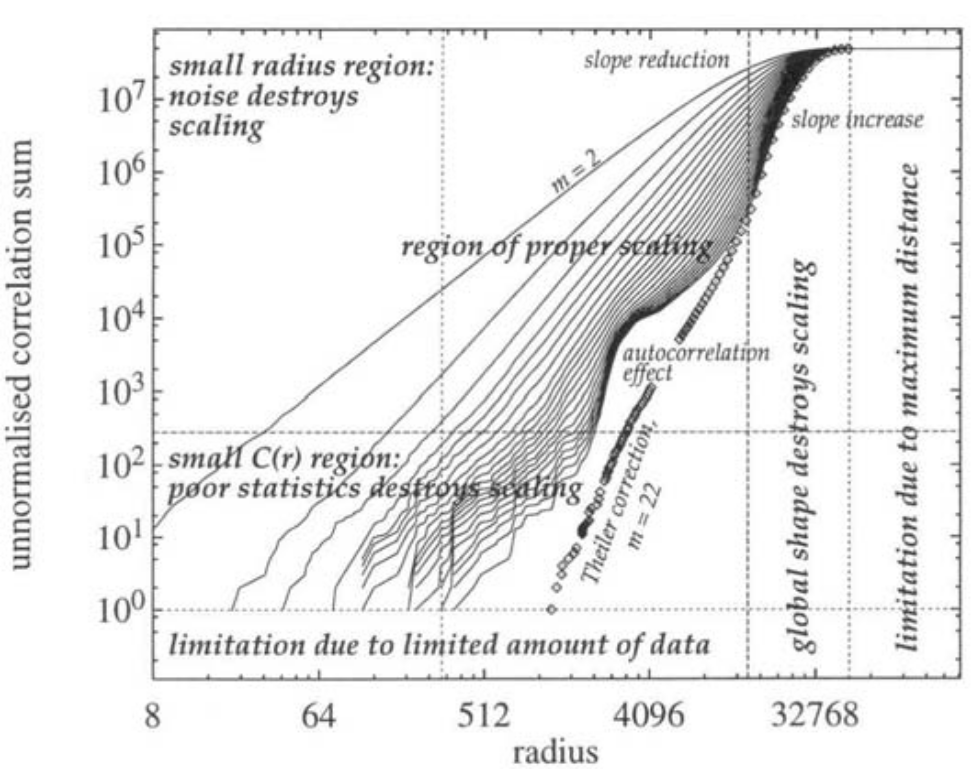
\includegraphics[width=0.6\textwidth]{Images/typ-cr.png} }
  \caption[Typical behavior of $C(r)$.]{Plot of typical behavior of the non-normalized corretion sum $C(r)$ with regions relevant to $D_2$ estimation (both axes are logarithmically scaled)~\cite{andreas2000}. It is important to observe that either too low or too high values of $r$ lead to poor estimation of the derivative: the former caused by statistical fluctuations, and the latter by the fact that the maximum pairwise distance is bounded. Using too high embedding dimension may also lead to poor estimations due to autocorrelation effects (an umbrella term for effects due to sampling and nonstationarity). To compare with our results, see Figure~\ref{fig:cr}. }
\label{fig:exp-cr}
\end{figure}

In our experiments, we used \emph{local slopes approach} to estimating the correlation dimension, which is based on the idea of assigning a dimension estimate to each value of $r$ by defining
\begin{align} \label{eq:d2-partial}
  D_2(r) = \frac{\partial \log C(r)}{\partial \log r}.
\end{align}
In our implementation, we perform a least squares fit of values $(\log r, \log C(r))$ for a window of 6 neigboring points for each sampled $r$. Expected behavior of the resulting function in a favorable case can be seen in Figure~\ref{fig:exp-localcr}.

\begin{figure} 
\centering
\noindent\makebox[\textwidth]{%
  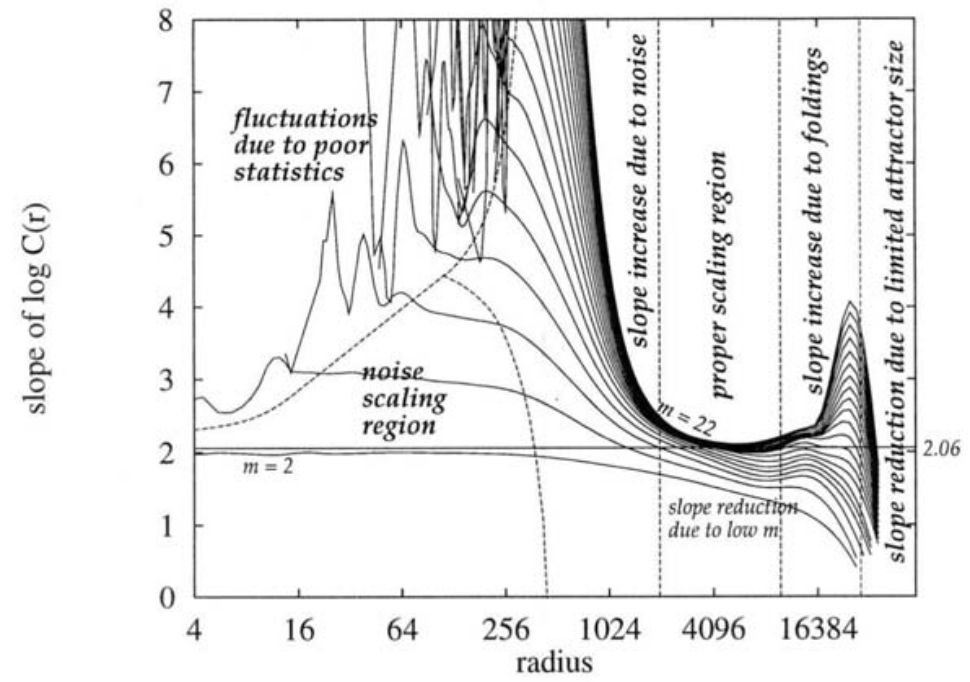
\includegraphics[width=0.6\textwidth]{Images/typ-localcr.png} }
  \caption[Typical behavior of local $D_2$ in favorable case.]{Plot of a typical local correlation dimension estimates for embedding dimensions from $m=2$ to $m=22$ (from bottom to top) in favorable case~\cite{andreas2000}. Note mainly the scaling region where the slope estimates converge to the value of $2$. To compare with our results, see Figure~\ref{fig:loc-d2}. The results has been generated using time series with 1600 datapoints.}
\label{fig:exp-localcr}
\end{figure}

\subsubsection{Dataset Size Requirements} \label{sec:req-corr}
There are multiple estimations of the minimum dataset size. Most of them are based on an attempt to avoid so called \emph{edge effect}. It can be shown that the correlation dimension for a hypercube in $m$-dimensions of unit edge length the local correlation dimension is
\begin{align*}
  D_2^{(m)}(r) = m - \frac{mr}{2-r} \approx m(1 - \frac{r}{2}).
\end{align*}
For large enough $r$, $D_2^{(m)}(r)$ converges to zero. This result, which can be generlized to any finite object, is a consequence of the discontinuity of the measure (\ref{eq:measure}) at the boundaries of the hypercube. Theiler, assuming evalution of the local correlation dimension for radius where each point has on average one neighbor (such that $C(r) = 1/N_{(m, \tau)}$), derived an estimate for the minimum data set size as
\begin{align*}
  N_{(m, \tau)} = \frac{1}{(4\rho)^m},
\end{align*}
where $\rho$ is the maximum error. This implies an exponential increase of minimum required dataset size with embedded dimension. For example, $N_{(m, \tau)} = 5^m$ for $\rho = 5\%$~\cite{andreas2000}.

\subsection{Detrended Fluctuation Analysis} \label{sec:dfa-theory}
Physiological time series, such as EEG, may exhibit so called statistical self-affine properties. Self-affinity is a special case of self-similarity, which occurs when one or more small parts of a fractal object is exactly or approximately similar to itself. When self-similarity is expressed in terms of statistical properties (e.g. mean value and variance of a part of time series are scaled version of its overall mean and variance), then the object is called statistically self-similar.\footnote{An example of statistically self-similar object are are naval coastlines.} Self-similarity, in turn, differs from self-affinity in that self-affine objects witness similarity anisotropically, i.e. after applying an anisotropic affine transformation.\footnote{The measured property of a self-similar process (e.g. the size of a flower on Romanesco cauliflower) do not follow normal distributions, but power law distributions. Hence, mode and mean of provide a poor representation of this representation. These processes do not have a scale at which to measure these statistics to characterize them, and are therefore called scale-free.}~\cite{hardstone2012detrended} Stated more formally:

\begin{dfn}[\cite{beran2017statistics}] \label{def:self-affin}
  A time series $X$ given by $x_1, x_2, \dots, x_n$ is said to be \textbf{statistically self-affine} if 
  \begin{align*}
    \mathrm{std}(X, Lt) \approx L^H \mathrm{std}(X, t),
  \end{align*}
  where $\mathrm{std}(X,k)$ is the standard deviation of the process $X$ calculated over windows of length $k$, $H$ is the Hurst parameter, and L a window length factor.
\end{dfn}

The Hurst parameter, which behaves similarly to the Hurst exponent (see Section~\ref{sec:hurst-theory}), ranges between 0 and 1. Higher values of $H$ describe smoother signals, with high values followed by low, whereas low values of $H$ indicate radical oscillations between high and low values. Note that since a stationary process has constant variance across time scales, Definition~\ref{def:self-affin} applies only to nonstationary processes. However, even stationary processes may exhibit scale-free behavior. These are modelled as so called fractional Gaussian noise (fGn), whereas nonstationary processes are modelled as fractional Brownian motion (fBm). These processes are related by the fact that increments in fBm can be modelled as a fGn process with same $H$. This relationship allows us to generalize Definition~\ref{def:self-affin} for nonstationary processes~\cite{hardstone2012detrended}.

DFA is a method of estimating $H$ without making prior assumptions about stationarity of the process by exploiting the relationship between fGn and fBm procesess. First, a so called signal profile, i.e. integral of the de-meaned signal is computed as
\begin{align*}
  y_k = \sum_{i=1}^{k} \left( x_i - \langle x \rangle \right).
\end{align*}
The resulting time series $y$ is then divided into segments of varying length $n$ (each value of $n$ representing a time scale). A local linear least-squares fit is applied to each of these segments. Let us designate the resulting piecewise linear fit as $y_n(k)$. The integrated time series is then detrended by subtracting the local linear fit. The root mean square error is then given by 
\begin{align} \label{eq:dfa-fm}
  F(n) \coloneqq \sqrt{ \frac{1}{N} \sum_{i=1}^{N} \left( y_i - y_n(i) \right)^2 }.
\end{align}
Finally, if a log-log plot $F(n)$ as a function $n$ shows a linear scaling region (i.e. the original time series exhibits self-similar, scale-free properties described above), the slope of this line approximates $H$ and represents the result of DFA analysis~\cite{lee2007detrended}.

\add[inline]{Maybe add some more intuitive explanation.}

The importance of DFA for EEG analysis comes from the observation that it can reveal so called long-range temporal correlations (LRTC) in neuronal activity, and so even for nonstationary time series~\cite{lee2007detrended}. This is especially important because EEG signals are nonstationary in some cases, and, as we will see in Section~\ref{sec:corrdim-anal}, some other frequently used measures, such as LLE and CD, theoretically depend on stationarity property. 

Long-range temporal correlations, or long-range dependence, is a phenomenon which occurs when the average rate of decay of statistical dependence between increasingly (temporally) distant points in the time series is slower than exponential. Large-scale patterns in EEG activity may be characteristic of baseline processing during eyes-closed wakeful condition in healthy human brain. These parameters computed from the theta amplitudes were shown to be negatively correlated with (Hamilton) depression score, thus suggesting that depressed patients display abnormally small autocorrelations on large scale~\cite{linkenkaer2005breakdown}. In our study, we observed similar results, see Section~\ref{sec:analdepdif}.

\subsection{Hurst Exponent} \label{sec:hurst-theory}
As mentioned in the previous section, similarly to the Hurst parameter in DFA, Hurst exponent is a measure of presence of long-range temporal dependencies in the time series. It was developed from Edwin H. Hurst observation when researching the optimal (or minimal required) storage sizing of river dams. Supposing there is a constant reservoir outflow equal to the mean annual water discharge, required storage size corresponds to the range (i.e. the difference between the maximum and the minimum value) of a cumulative sums of deviations from the mean annual discharge. We shall call this value, as a function of the number of years, $R(n)$~\cite{hurst1956problem}. After manually analyzing about a hundred records of natural phenomena, Hurst was able to demonstrate this value, on average and after normalizing by the standard deviation of the original time series, follows the following trend:
\begin{equation} \label{eq:resc-range}
  R(n) / \mathrm{std}(n) \propto (n / 2)^K.
\end{equation}
In this equation, $R(n) / \mathrm{std}(n)$ is called the rescaled range, and $K$ is called the Hurst exponent~\cite{hurst1957suggested}. Obviously, it is always the case that $0 \leq K \leq 1$.

The algorithm we used for computing estimation of the Hurst exponent is as follows~\cite{weron2002estimating}. Let us have time series $x$, with values $x_1, x_2, \dots, x_N$. The time series is split into $d$ non-overlapping subseries $x^{(m)}$, $m\in 1,2,\dots,d$ of fixed length $n$. Sample mean $\langle x^{(m)} \rangle$ and standard deviation $\mathrm{std}(m)$ is computed for each. Each subseries $x^{(m)}$ is then normalized, and cumulative time series is computed as 
\begin{align*}
  z_k^{(m)} &= \sum_{i=1}^{k} (x_i^{(m)} - \langle x^{(m)} \rangle) \qquad \mathrm{for }\, k=1,\dots,n .
\end{align*}
Range $R(m)$ is then computed for each subseries as
\begin{align*}
  R(m) &= \max_{i=1,\dots,n}{z_i^{(m)}} - \min_{i=1,\dots,n}{z_i^{(m)}}.
\end{align*}
Then, the mean value of the rescaled range
\begin{align}\label{eq:hurst-mean}
  (R/S)_n = \frac{1}{d} \sum_{m=1}^d R(m)/S(m)
\end{align}
is computed. This procedure is performed for chosen values of $n$. As observed by Hurst~\cite{hurst1956problem}, and later proven by Mandelbrot~\cite{mandelbrot1975limit}, the rescaled range asymptotically follows the relation
\begin{align*}
  (R/S)_n \propto cn^K.
\end{align*}
The Hurst exponent $K$ then can be obtained using linear regression as slope of the line
\begin{align} \label{eq:hurst-rs}
  \log (R/S)_n = \log c + K \log n .
\end{align}

Interestingly, if the measured quantites resulted from mutually completely independent events (i.e. white noise, with its corresponding cumulative sum, random walk), the relationship in equation (\ref{eq:resc-range}) is replaced with
\begin{equation*}
  R(n) / \mathrm{std}(n) \propto 1.25 \sqrt{N},
\end{equation*}
as can be easily verified by flipping a set of coins.\footnote{Hurst himself actually made experiments, tossing 10 coins 1000 times. It took him almost 6 hours~\cite{feder2013fractals}.}~\cite{hurst1957suggested} This allows us to recognize stochastic processes with mutually uncorrelated values. The value of Hurst exponent for white noise is $K=1/2$, and many natural processes, such as rainfalls, river water level heights, temperatures and pressures, annual growth of tree rings, and even financial markets have $K > 1/2$, suggesting long-term temporal correlations in the processes. Values of $0 \leq K < 1/2$, on the other hand, suggest long-time negative correlations, i.e. high values being often followed by low values in the future~\cite{hurst1956problem}.

\subsection{Higuchi's fractal Dimension} \label{sec:hd-theory}
In this section, it will be beneficial to change our usual notation for the purpose of readability. Let us have time series $x(1), x(2), \dots, x(N)$. We select a $k \in \NN$ and construct $k$ new time series, denoted $x_k^m$ for $m=1,2,\dots,k$, as 
\begin{align*}
  x(m), x(m+k), x(m+2k), \dots, x(m + \floor{\frac{N-m}{k}} \cdot k), \qquad m=1,2,\dots,k, \qquad m,k \in \NN,
\end{align*}
where $m$ is represents the initial time, and $k$ the interval time. In this way, we sample $k$ subseries where the delay between successive points, or $\mathrm{size}$ in equation (\ref{eq:dim-intuitive}), is precisely $k$ for each. Then, we define normalized average length $L_m^k$ of each $x_k^m$, or its $\mathrm{bulk}$ in equation (\ref{eq:dim-intuitive}), as follows
\begin{align*}
  L_m^k = \left( \sum_{i=1}^{\floor{\frac{N-m}{k}}} | x(m+ik) - x(m+(i-1)k) | \right) \frac{N-1}{\floor{\frac{N-m}{k}} \cdot k},
\end{align*}
where $\frac{N-1}{\floor{\frac{N-m}{k}} \cdot k}$ is a normalization factor. Length of the original curve as a function of $k$ is then defined as the average $L(k) \coloneqq \langle L_m^k \rangle_m$ over $k$ values of $L_m^k$. If $L(k) \propto k^{-D_H}$ for some value of $D_H$, then the curve can be considered fractal with fractal dimension $D_H$, which can be estimated by least-squares fitting the logarithm of the length $\log{L(k)}$ as a function of $\log{k}$~\cite{higuchi1988approach}.

In summary, Higuchi's fractal dimension can be defined, in analogy with correlation dimension and equation (\ref{eq:d2-partial}), as
\begin{align*}
  D_H = -\frac{\partial \log{L(k)}}{\partial \log{k}}.
\end{align*}
In other words, one may see Higuchi's fractal dimension as measure of irregularity, which in turn is measured as logarithmic rate of average variation of successive points~\cite{ahmadlou2012}. Comparing with equation (\ref{eq:dim-intuitive}), can see that $\mathrm{bulk}$ is corresponds to the mean curve length over multiple subsampled time series $L(k)$ as a function of their $\mathrm{size}$, which is the delay length $k$. 

In comparison with correlation dimension, one of the benefits of Higuchi's fractal dimension is its relatively fast computation.

\subsection{Sample Entropy} \label{sec:se-theory}
Understood in the context of dynamical systems, entropy is the rate at which a given system produces information. It is equal to the sum of all positive Lyapunov exponents of the system's attractor, and positive entropy indicates presence of chaotic dynamics~\cite{andreas2000}. Computing entropy from a physiological time series directly using the information-theoretical definition, is, however, problematic. The time series produced during measurements on biological systems are often short and noisy. Moreover, in EEG analysis, the impact of noise is especially severe. To combat this issue, many methods of computing entropy for such time series has been devised. Sample entropy represents an improvement~\cite{richman2000physiological} on other entropy measure popular in clinical settings, called approximate entropy, which has been successfully applied on EEG to classify diseases such as schizophrenia, epilepsy, and addiction~\cite{yun2012decreased}.

For a given embedding dimension $m$ and tolerance parameter $r$, sample entropy can be defined as the negative natural logarithm of the conditional probability that two subseqences of the time series of length $m$ which are similar, i.e. their distance is less than $r$ (excluding self-matches\footnote{This is one of the differences of sample entropy from approximate entropy.}), will remain similar after including the next point, i.e. when their respective lengths are increased to $m+1$. Thus, sample entropy is a measure of predictability, lower value of sample entropy indicates more self-similarity, or, in a certain sense, less complexity. More concrete definition may be stated as follows:
\begin{dfn}[\cite{richman2000physiological}]
  Let us have a time series $x_1, x_2, \dots, x_N$, and let $\mathbf{x}_i^{(m)} = \left( x_i, x_{i+1}, \dots, x_{i+m-1} \right)$ be the $i$-th vector in the embedding of dimension $m$, and $\norm{\cdot}_{\infty}$ be the Chebyshev metric\footnote{Any metric can be used, but Chebyshev metric is recommended by the original authors~\cite{richman2000physiological}.}. Then, \textbf{sample entropy} is defined as
  \begin{align*}
    \mathrm{SE}(m, r) = -\ln \frac{A^m(r)}{B^m(r)},
  \end{align*}
  where
  \begin{description}
    \item[$A^m(r)$] is the number of vector pairs in the embedding satisfying $\norm{\mathbf{x}_i^{(m+1)} - \mathbf{x}_j^{(m+1)}}_{\infty} < r$, $i \neq j$, and 
    \item[$B^m(r)$] is the number of vector pairs in the embedding satisfying $\norm{\mathbf{x}_i^{(m)} - \mathbf{x}_j^{(m)}}_{\infty} < r$, $i \neq j$.
  \end{description}
  We call the value $r$ \emph{tolerance}.
\end{dfn}
Obviously, it is always $A^m(r) \leq B^m(r)$, hence sample entropy is always non-negative. If $A^m(r) = B^m(r)=0$, no regularity has been detected, and $B^m(r) \neq 0$ with $A^m(r)=0$ corresponds to (the above mentioned) conditional probability of 0, and infinite value of sample entropy. The value of tolerance $r$ recommended by the authors is $0.2 * \mathrm{std}(x)$, where $\mathrm{std}(x)$ is the standard deviation of the original time series~\cite{richman2000physiological}.

The algorithm for computing sample entropy first constructs the embedding vectors for embedding dimensions $m$ and $m+1$. For each embedding dimension, it counts the number of pairs of vectors $\mathbf{x}_i, \mathbf{x}_j$ where $i \neq j$, for which $\norm{ \mathbf{x}_i - \mathbf{x}_j }_{\infty} < r$. The negative natural logarithm of the ratio of number of those pairs for dimension $m+1$ and the number of pairs for dimension $m$ is the result.

Sample entropy has been successfully employed for diagnosing depression~\cite{acharya2015novel, hauge2011nonlinear}. It was shown to be significantly different between middle aged and elderly women during sleep~\cite{bruce2009sample}. \add{Extend this section a little bit.}

\section{Surrogate Data Testing} \label{sec:surrogate-analysis-theory}
It has been shown that, for example, fitered noise can mimic low-dimensional chaotic attractors when examined by Grassberger-Procaccia algorithm described above In the following, we will describe a method for answering this question. \info{We may also want to know whether the process is determinsitic or not. There are tests for that, but we are not using them in this thesis.}

To this end, we construct a Monte Carlo hypothesis test of nonlinearity. We choose a null hypothesis of a model for the process creating obtained data which denies the property we assume to measure. For each time series, we create so called \emph{surrogate data} which deliberately capture only properties consistent with chosen null hypothesis, and compute the estimates using the same method as for the original data. If the result for the original time series is significantly different from the surrogate estimates, we reject the the null hypothesis. In the opposite case, we fail reject the null hypothesis. A schematic depiction of the process can be seen in Figure~\ref{fig:surr-schema}.

\begin{figure} 
\centering
\noindent\makebox[\textwidth]{%
  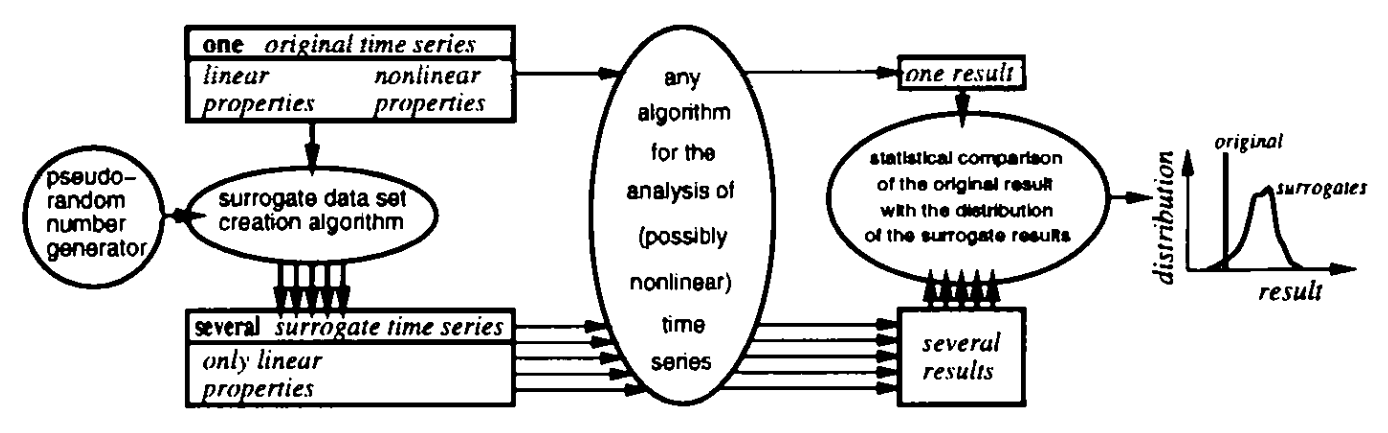
\includegraphics[width=0.8\textwidth]{Images/surr_schema.png} }
  \caption[Illustration of surrogate data testing process.]{A schematic depiction of surrogate data testing process for the null hypothesis of a linear process~\cite{andreas2000}.}
\label{fig:surr-schema}
\end{figure}

Here, we use two sided test, and measure of significance is defined as
\begin{align} \label{eq:sigma}
  \mathcal{S} \equiv \frac{| Q_{\text{orig}} - \mu_{\text{surr}} |}{\mathrm{std}_{\text{surr}}},
\end{align}
where $Q_{\text{orig}}$ is the statistic computed for the original time series, and $\mu_{\text{surr}}$, $\mathrm{std}_{\text{surr}}$ are the mean and standard deviation of the statistic computed for the surrogate time series~\cite{theiler1992testing}. If we assume that distribution of the generated is Gaussian, than $\mathcal{S} \geq 2$ is required for 95 \% significance level. However, validity of this assumption is not always guaranteed. For non-Gaussian distributions, we may require larger $\mathcal{S}$, or, alternatively, use a rank based test, as follows~\cite{kantz2004}.

Using rank-based test, we want to test if $Q_{\text{orig}}$ is smaller or larger than the expected value of estimates produced by the null hypothesis model. If we generate $n_s$ surrogate estimates, then, we have $n_s$ estimates following the null hypothesis, each having a probability $2/n_s$ of being the smallest or largest. A false rejection will happen if $Q_{\text{orig}}$ happens to also follow the null hypothesis and is either the smallest or the largest, which happens with probablity $1 - \alpha \coloneqq 2/(n_s+1)$, where $\alpha$ is the confidence level. Hence, for confidence level $\alpha = 95 \%$, the number of surrogates should be $n_s = 38$~\cite{andreas2000}. Note that, since many of the algorithms used for estimating nonlinear measures are relatively computationally expensive, surrogate analysis with high confidence levels, especially on large datasets of multichannel signals such as EEG, is even more so.

\subsubsection{Generating Improved Amplitude Adjusted Surrogates} \label{sec:iaaft}
For our purposes, since we assume that the data are produced by a nonlinear process, a reasonable null hypothesis may be that the data are produced by a Gaussian linear stochastic process $\mathrm{AR}(p)$
\begin{align} \label{eq:lin-stoch-proc}
  x_{t+1} = \mu + \sum_{j=0}^{p-1} a_j x_{t-j} + \sigma e_t,
\end{align}
with unknown parameters $a_j, e_t, \mu, \sigma \in \RR$~\cite{theiler1992testing}.

If the computed nonlinear statistic depends on the free parameters in $\mathrm{AR}(p)$ (\ref{eq:lin-stoch-proc}) (which is not true, e.g. for $D_2$), then one may try to estimate these parameters from the original time series. Alternatively (and this is the approach we use in our analysis), one may exploit the fact that $\mathrm{AR}(p)$ can be also perfectly described by its power spectrum~\cite{theiler1992testing}.\footnote{This is due to Wiener-Khinchin theorem, which states, roughly, that spectral decomposition of autocorrelation of a stationary process is the power spectrum of the process.} Hence, to obtain a surrogate, one may simply perform a Fourier transform of the original time series, randomize phases, and apply inverse Fourier transform. This way, the amplitudes (composing the power spectrum) are preserved. This procedure has been named \emph{Fourier transform phase randomization} (FTPR).

However, there is a drawback of FTPR. It has been shown that if the amplitudes of $\mathrm{AR}(p)$ are not Gaussian (as in (\ref{eq:lin-stoch-proc})), e.g. nonlinear,\unsure{e.g. or i.e. here?} then the surrogates created using this method show nonlinear behavior~\cite{kantz2004}. Rarely do the amplitudes of an experimental process follow a Gaussian distribution. Hence, we change our model to correspond a nonlinear, time independent filter applied to the output of $\mathrm{AR}(p)$. Surrogate creation algorithm for this model was described by Theiler in~\cite{theiler1992testing}: rescale the values of the original time series so that they are Gaussian, apply FTPR described above, rescale the values back to follow the same distribution of the original time series. This surrogate creation method is called \emph{amplitude-adjusted Fourier transform} (AAFT), and has been successfully applied to EEG signal~\cite{theiler1994evidence}.

Even this method is not without its drawbacks: due to the final reordering, the original power spectrum is slightly distorted in the surrogate. In~\cite{theiler1994evidence}, it was proposed how to mitigate this effect. The amplitudes of Fourier transform of AAFT surrogates are replaced by the amplitudes of the original time series. The power spectrum is now correct, but the distribution is wrong. So, the original time series is reordered to according to ranks of values in this surrogate. This results in precisely the desired distribution of values, but again, slightly deviant power spectrum. These steps are then iterated and, experimentally, they results seem to converge. Hence, the final procedure, called \emph{improved (iterated) amplitude-adjusted Fourier transform} (iAAFT) can be summarized as follows:~\cite{andreas2000}

\add[inline]{Maybe talk about the problems, e.g. endpoint mismatch? We will need to refer to them later.}

\begin{enumerate}[label*=\arabic*.]
  \item Compute and store the moduli of the original time series.
  \item Create an AAFT surrogate as follows:
    \begin{enumerate}[label*=\arabic*.]
      \item Create a set of random numbers with Gaussian distribution.
      \item Rank order the original time series (or the one obtained in step 5.), and reorder the random numbers created in the previous step such that they achieve the same ordering as the original time series.
      \item Randomize the phases Fourier transform of the time series obtained in previous step and apply inverse Fourier transform.
      \item Find the rank ordering of the time series obtained in the previous step, and reorder the original time series so that it assumes the same rank ordering.
    \end{enumerate}
  \item Replace the moduli of these surrogates by those of the original time series and apply inverse Fourier transform.
  \item Find the rank ordering of the time series obtained in the previous step, and reorder the original time series so that is assumes the same rank ordering.
  \item Apply step 2. to time series obtained in the previous step, or stop if stopping criterion is reached.
\end{enumerate}

\section{Practial Applications}
\subsection{Applications in Depression Diagnosis}\label{sec:applications}
\subsubsection{Nonlinear Measures}
Although nonlinear dynamical analysis of EEG signal has been successfully applied to many psychological and psychiatric conditions, such as insomnia, schizophrenia, epilepsy, dementia, Alzheimer's disease, the number of studies applying methods of nonlinear time series analysis for clinical depression diagnosis is still relatively limited~\cite{stam2005, rodriguez2015}. Summary of studies reviewed in this section along with the obtained results can be seen in Table~\ref{tab:depsum}. Hereby we present the studies in chronological order.

It has been found that the EEG dynamics of depressed patients exhibit more predictability, and therefore less complexity, than those of non-depressed ones, with this indicator receding after treatment~\cite{nandrino1994, pezard1996}. Instead of measuring compexity using correlation dimension, the authors applied method of nonlinear forecasting of dynamical systems based on the local approximation of neighborhood evolution~\cite{nandrino1994}.

Another study analyzed sleep EEGs of depressed and control subjects, and found significantly decreased values of Lyapunov exponents in a sleep stage IV in depressed patients relative to control~\cite{roschke1995nonlineardeppression}.

In 2007, Lee et al. found significant differences between the values of DFA in 11 depressed patients matched with the same number of healthy controls. Moreover, they found signiciant correlation between the values of DFA and depression scores in almost all recorded channels~\cite{lee2007detrended}. 

In 2012, Ahmadlou et al. decomposed 5 EEG channels recorded from frontal lobes of healthy and depressed patients using wavelet filter banks, measured their complexity using Higuchi's fractal dimension, subsequently used ANOVA to discover the most meaningful differences between the groups, and trained a probabilistic neural network classifier, achieving 91.3\% classification accuracy on limited amount of data. This research suggested potential of frontal lobe signal assymetry as a measure for depression~\cite{ahmadlou2012}.

A year later, Hosseinifard et al. extracted Correlation Dimension (CD), the Largest Lyapunov Exponent (LLE) and Higuchi's fractal Dimension (HD) from 4 EEG channels of 90 patients split evenly between depressed and non-depressed subjects, achieving 90\% accuracy using a logistic regression classifier and 3-fold leave-one-out cross validation~\cite{hosseinifard2013}.

In the same year, Bachmann et al. compared linear measure called Spectral Assymetry index (SASI) and HD for depression diagnosis on 34 subjects split evenly between depressed and control group. SASI achieved true detection rate in 88\% in depressives and 82\% in the controls, while HD provided true detection rate of 94\% in the depressives and 76\% in the controls~\cite{bachmann2013}, thus both giving comparable results.

In 2014, sample entropy, approximate entropy, Renyi entropy and bispectral phase entropy were used by Faust et al. in~\cite{faust2014depression} to achieve overall 99.5\% accuracy using 10-fold cross validation on sample of 30 healthy and 30 depressed patients. This study reports the highest accuracy out of the reviewed studies. 

A year later, Acharyia et al. invented a new biomarker based on nonlinear measures called Depression Diagnosis Index (DDI) and also achieved considerable accuracy, but on a small sample of 15 depressed patients matched with healthy controls~\cite{acharya2015novel}.

In comparison with depression diagnosis, less research has been dedicated to the problem of treatment outcome prediction using nonlinear measures. The only study we are aware of is~\cite{arns2014non},  where the authors computed LLE using false nearest neighbors and another nonlinear measure called Lempel-Ziv Complexity (LZC) in order to investigate depressed patients' response to treatment with repeated Transcranial Magnetic Stimulation (rTMS). They observed a significant decrease in LZC in nonresponding patients and significant increase in responding patients and healthy controls. 


\subsubsection{Other Techniques}
Most of the results of applications of quantitative methods to EEG analysis of depressed patients were obtained using linear methods, such as extracting band power features to detect assymetries between hemispheres of the brain~\cite{rodriguez2015}. For example, in~\cite{knott2001eeg}, the researchers were able to distinguish between 23 healthy and 70 depressed patients using only linear measures\footnote{Note however the class imbalance in the study.}. Statistically significant differences between depressed patients and healthy controls using anterior $\alpha$ assymetry were found in~\cite{debener2000resting}, followed by~\cite{omel2002changes} with more linear assymetry features and more substantial sample size and similar results. Moreover, statistically significant differences in relative frontal power were found in~\cite{iosifescu2009frontal} between depressive patients responding and nonresponding to treatment. Puthankattil et al. were able to obtain high 98.1\% accuracy using relative wavelet energy and neural networks on a sample of 30 healthy and 30 depressed patients. Each patient was recorded multiple times to increase the size of the training and test sample, which may have introduced correlations between the training and test sets. Nonetheless, these studies, supported by neuroscientific theory, sparked interest in linear assymetry measures in depression diagnosis.

However, many studies cast doubts over validity of these measures, such as~\cite{hinrikus2009electroencephalographic, allen2004stability, ahmadlou2013spatiotemporal} finally followed by~\cite{gold2013validity} in 2013 with more substantial sample size, all either finding no statistically significant differences between depressed patients and healthy controls, or no statistically significant correlations of assymetry measures with depression scores. Moreover, when compared directly to nonlinear measures, linear techniques seem to perform at most comparably to nonlinear ones, or worse. As already mentioned, in~\cite{bachmann2013}, nonlinear measure HD was comparably discriminative to linear measure of spectral assymetry. In~\cite{hosseinifard2013}, Hosseinifard et al. obtained lower classification accuracy using linear band power features in comparison to CD, LLE, and HD. 

In attempt to discriminate between MDD patients responding and nonresponding to rTMS treatment, in~\cite{arns2012neurophysiological}, the researchers identified increased frontal $\theta$ power and lower peak $\alpha$ frequency as potential biomarkers for patient's failure to respond to the treatment. 

Considerably more research has been devoted to the problem of treatment outcome prediction using linear measures in comparison with nonlinear measures. However, most of the studies include only small number of samples and tend to limit their focus on a specific biomarkers~\cite{olbrich2013eeg}. For a comprehensive review, see~\cite{olbrich2013eeg}.

\subsubsection{Potentially Related Diseases}
Sleep disorder diagnosis may also relevant to this work for the very close connection of depression with disturbed sleep and insomnia~\cite{nutt2008}. The first study emplying techniques of nonlinear analysis on human EEG was published in 1985 and dealt with sleep recordings~\cite{babloyantz1985}. This early success sparked intensive research focus on applying nonlinear analysis to sleep data, thus generating relatively large amount of results. 

Many studies focused on extracting Lyapunov exponents of EEGs measured during various sleep stages. The general pattern that emerged was that deep sleep stages exhibit lower complexity evidenced by lower fractal dimensionality and lower values of the largest Lyapunov exponent~\cite{stam2005}.

Recurrence plots, and RQA in particular, have been demonstrated to be effective at decoding neuroscientific physiological time series. For example, they have been suggested as a method of lowering signal-to-noise ratio in analysis of event related potentials in response to a surprising stimulus, where repeated exposure would influence the outcome (and thus classical averaging methods are not viable)~\cite{marwan2007recurrence}. Moreover, they have been successfully employed in detecting epileptic seizures using intracranial recordings~\cite{pijn1997nonlinear}. Simple K-nearest neighbors classifiers achieved surprisingly high accuracies at emotion recognition tasks~\cite{bahari2013eeg}, and convolutional neural networks used recurrence plots for activity recognition~\cite{garcia2018classification}. Most importantly for our study, recurrence plots of signals in the left hemisphere were observed to qualitatively differ between healthy baseline and depressed patients. The authors suggested that this area is worth further exploration~\cite{acharya2015computer}.

\begin{table}[ht]
\centering
\resizebox{\textwidth}{!}{\begin{tabular}{|c|c|c|c|c|c|c|c|c|}
\hline
\textbf{Measure} & \textbf{Analysis method} & \textbf{\spatcell{Accuracy or\\obtained results}} & \multicolumn{2}{c}{\textbf{Test sample}} \vline & \textbf{\# channels} & \textbf{Rec. length} & \textbf{Reference} & \textbf{Note} \\ \hline
 & & & \textbf{Healthy} & \textbf{Depressed} & & & & \\ \hline
 \spatcell{SE and other entropies} & WPD+PNN & 0.99 & 30 & 30 & 9 & 5 min &~\cite{faust2014depression} & \spatcell{Evaluated using 10f-CV.}\\ \hline
 DDI & SVM & 0.98 & 15 & 15 & - & 8 s &~\cite{acharya2015novel} & - \\ \hline
 HD & EPNN & 0.91 & 3 & 3 & 19 & 1 min &~\cite{ahmadlou2012} & - \\ \hline
 HD & LDA & 0.85 & 17 & 17 & 18 & 2 s &~\cite{bachmann2013} & Evaluated on training set. \\ \hline
 LLE, CD, DFA, HD & LR & 0.9 & 45 & 45 & 19 & 5 min &~\cite{hosseinifard2013} & - \\ \hline
 NL forecasting & Measuring predictability & \spatcell{Increased predictability\\in MDD patients} & 8 & 16 & 12 & 40 s &~\cite{nandrino1994} & - \\ \hline 
 LLE & Statistical analysis & Found s.s. diff. & 13 & 15 & 4 & 2.44 min &~\cite{roschke1995nonlineardeppression} & - \\ \hline
 DFA & Statistical analysis & Found s.s. diff. & 11 & 11 & 5 & 5 min &~\cite{lee2007detrended} & - \\ \hhline{|=|=|=|=|=|=|=|=|=|}
 RWE & NN & 0.98 & 40 & 40 & 9 & 5 min &~\cite{puthankattil2012classification} & - \\ \hline
 \spatcell{Power, assymetry,\\coherence measures} & Statistical analysis & 0.91 & 23 & 70 & 21 & 20 min &~\cite{knott2001eeg} & - \\ \hline
 Anterior $\alpha$-assymetry & Statistical analysis & Found s.s. differences & 15 & 22 & 19 & 2 s &~\cite{debener2000resting} & - \\ \hline
 Power and assymetry measures & Statistical analysis & Found s.s. differences & 86 & 53 & 8 & - &~\cite{omel2002changes} & - \\ \hline
 SASI & Statistical analysis & No s.s. diff. found & 18 & 18 & 9 & 2.5 s &~\cite{hinrikus2009electroencephalographic} & - \\ \hline
 FAA & Statistical analysis & No s.s. corr. found & - & 30 & 25 & 1 min &~\cite{allen2004stability} & \spatcell{FAA is stable in depressed\\patients, but uncorrelated\\with depression level.} \\ \hline
 STARC & Statistical analysis & No s.s. diff. found & 20 & 22 & 19 & 1 s &~\cite{ahmadlou2013spatiotemporal} & \spatcell{Focus is on classification\\ of male and female patients.} \\ \hline
 FAA & Statistical analysis & No s.s. corr. found & - & 79 & 32 & 2 s &~\cite{gold2013validity} & \spatcell{Measured correlations with\\depression scores.} \\ \hline
\end{tabular}}
\caption[Overview of reviewed depression studies.]{Overview of reviewed studies analyzing EEG in relation to depression, ordered by obtained classification accuracy (if applicable), otherwise chronological order was used. The first part corresponds to studies using nonlinear dynamical measures.\\Abbreviations: DDI - Depression Diagnosis Index, (EP)NN - (Enhanced Probabilistic) Neural Network, FAA - Frontal Alpha Assymetry, RWE - Relative Wavelet Energy, SASI - Spectral Assymetry Index, STARC - Spatiotemporal Analysis of Relative Convergence, WPD - Wavelet Power Decomposition, kf-CV - k-fold Cross Validation.}
\label{tab:depsum}
\end{table}

\subsection{Applications in Depression Prognosis} \label{sec:applications-prog}
In terms of EEG-based treatment outcome prediction, substantial effort has been devoted to examination of frontal $\theta$ frequencies, especially relative to $\alpha$ frequencies. This rationale is supported by several neuroscientific theories~\cite{hunter2007promise}. For example, in~\cite{iosifescu2009frontal}, the authors developed Antidepressant Treatment Index (ATR), a nonlinear combination of $\alpha$ and $\theta$ powers to predict treatment outcome with 63\% accuracy. The same research group had been examining relative $\theta$ powers for multiple years prior to this study, with the best results achieving 71\% accuracy on a dataset of 52 MDD patients~\cite{hunter2007promise}.

In~\cite{tenke2011current}, was used frequency principal component analysis derived from current source density waveforms to extract EEG $\alpha$ aplitude, achieving also 63\% accuracy. However, the highest accuracy of all reviewed studies was achieved using more advanced techniques in~\cite{khodayari2013machine}, where the authors extracted log Power Spectral Densities (PSD) levels at all frequencies of interest for each electrode, spectral coherence, mutual information, log ratios of left and right hemisphere powers and log ratios of anterior and posterior powers, and then Fisher discriminant ratio for feature selection and mixture of factors machine learning technique based on maximum likelihood for classification, finally achieving 88\% accuracy. Nevertheless, this result was obtained on a relatively small dataset of 22 patients.

\begin{table}[ht]
\centering
\resizebox{\textwidth}{!}{\begin{tabular}{|c|c|c|c|c|c|c|c|c|}
\hline
\textbf{Measure} & \textbf{Analysis method} & \textbf{\spatcell{Accuracy or\\obtained results}} & \multicolumn{2}{c}{\textbf{Test sample}} \vline & \textbf{\# channels} & \textbf{Rec. length} & \textbf{Reference} & \textbf{Treatment} \\ \hline
 & & & \textbf{Responding} & \textbf{Nonresponding} & & & & \\ \hline
 \spatcell{Power, coherence, mutual\\information measures} & MFA & 0.88 & 7 & 15 & 16 & 60 s &~\cite{khodayari2013machine} & SSRI \\ \hline
 Frontal $\theta$ power & ATR & 0.63 & 45 & 37 & 4 & 2 s &~\cite{iosifescu2009frontal} & SSRI \\ \hline
 Average $\alpha$ amplitude & \spatcell{Measure above median\\of controls} & 0.63 & 28 & 13 & 67 & 2 min &~\cite{tenke2011current} & SSRI \\ \hline
\end{tabular}}
\caption[Overview of reviewed response studies.]{Overview of reviewed studies analyzing EEG in relation to response, ordered by obtained classification accuracy (if applicable), otherwise chronological order was used.\\Abbreviations: ATR - Antidepressant Treatment Index, MFA - Mixture of Factors}
\label{tab:respsum}
\end{table}

\subsection{Limitations} \label{sec:nl-limit}
Some authors suggests that the since most plausible research target for explaining the brain dynamics are the assemblies of coupled and synchronously active neurons, and since majority of those assemblies are describable by nonlinear differential equations, principles derived from nonlinear dynamics are applicable to characterization of these neuronal systems~\cite{kaplan2005}. The approach of estimating a finite embedding dimension (see Section~\ref{sec:state-space-reconstruction}), however, has been doubted by some of the most prominent figures in the field of nonlinear dynamical analysis, such as the originators of Grassberger-Procaccia algorithm (see Section~\ref{sec:corrdim})~\cite{grassberger1986climatic, procaccia1988complex}, followed by many others later~\cite{skinner1994low, rapp1995there, andreas2000}. With the exception in the case of epileptic seizures~\cite{stam2005}, there is very little evidence for the seemingly improbable hypothesis that such complex system with many extrinsic influences and interactions, such as the brain, would exhibit a level of comlexity comparable to e.g. a Lorenz system. The observed estimates of low dimension may due to artifacts or limited data size~\cite{grassberger1986climatic, procaccia1988complex}. 

On the other hand, as we will see in Section~\ref{sec:applications}, the techniqes derived from these theories still provide some useful information and are successfully applied in many practical situations. Therefore, it seems to be the case that indeed, brain dynamics are much more complex than we are forced to assume based on the theory, but nonlinear dynamical analysis still manages to capture some of its important aspects. Some researchers argued that these observations ask for reinterpratation of those results~\cite{albano1993reliability}, whereas others call for development of new measures which reflect the ongoing progression in understanding of brain dynamics~\cite{stam2005}.

\chapter{Nonlinear Analysis Approach} \label{ch:nonlin-approach}
\section{Dataset} \label{sec:dataset}
The dataset was provided by the \href{http://www.nudz.cz/en/}{Czech National Institute of Mental Health}, and the recording was performed by the institution's local specialists. It comprises of 133 subjects, 104 women and 29 men, ranging in age from 30 to 65 (47.7 $\pm$ 9.58).\footnote{We use the notation $\text{mean} \pm \mathrm{std}$.} Handedness was not recorded. Montgomery-Asberg Depession Rating Scale (MADRS)~\cite{williams2008development} questionnaire assessed by a trained psychologist was used to measure depression severity. This psychometric measurement results in a depression score ranging from 0 (normal) to 40 (severe depression), usually with the following cutoff points~\cite{herrmann1998sunnybrook}: 
\begin{description}
  \item[0 - 6]: symptom absent,
  \item[7 - 19]: mild depression,
  \item[20 - 34]: moderate depression,
  \item[34 - 40]: severe depression.
\end{description}
 
The experiment lasted 4 weeks. At the beginning of week 1, each subject's depression score was measured, their EEG signal was recorded, and, based on the measurement and patient's history, prescription of up to 4 treatments (drugs or rTMS) was made. After 4 weeks, depression score was remeasured and EEG signal recorded again.

During the EEG recording, 19 electrodes were placed on the scalp in accordance with the Internation 10-20 system (FP1, FP2, F3, F4, C3, C4, P3, P4, O1, O2, F7, F8, T3, T4, T5, T6, Fz, Cz, Pz), see Figure~\ref{fig:electrodes} for reference. EEG signals of 99 subjects were recorded at sampling frequency $f_s$ of 250 Hz, while 1000 Hz was used for the remaining 34 patients. The patients were not told to close their eyes for the duration of the recording, resulting in unwanted artifacts in the signal. Some of the artifacts were removed manually by the researchers by omitting those parts from the recording, and concatenating the remaining parts. Durations of the resulting measurements range from 23.5 s to 170 s (75.6 $\pm$ 20 s) for $f_s = 250$ Hz, and from 48.8 s to 140.4 s (79.5 $\pm$ 18.4 s) for $f_s = 1000$ Hz. The distributions of depression scores, EEG recording durations, patients' ages and sexes are visualized in Figure~\ref{fig:dataset-viz}. A typical recoding can be seen in Figure~\ref{fig:data}.

\begin{figure} 
\centering
\noindent\makebox[\textwidth]{%
  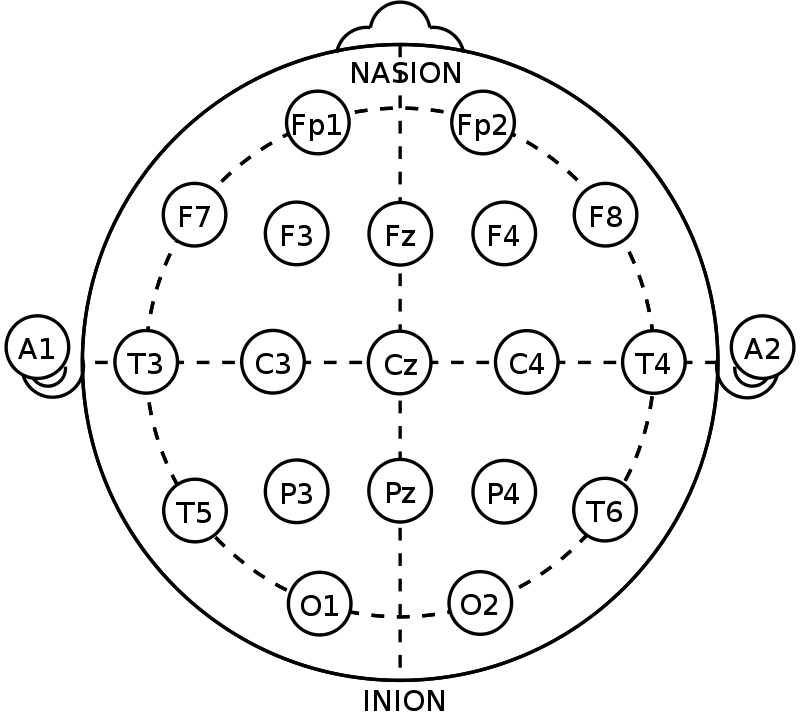
\includegraphics[width=0.5\textwidth]{Images/electrodes.png} }
  \caption[International 10-20 electrode placement system.]{The International 10-20 system for placement of EEG electrodes used in our dataset. (\cite{10-20-system})}
\label{fig:electrodes}
\end{figure}

\begin{figure} 
\centering
\noindent\makebox[\textwidth]{%
  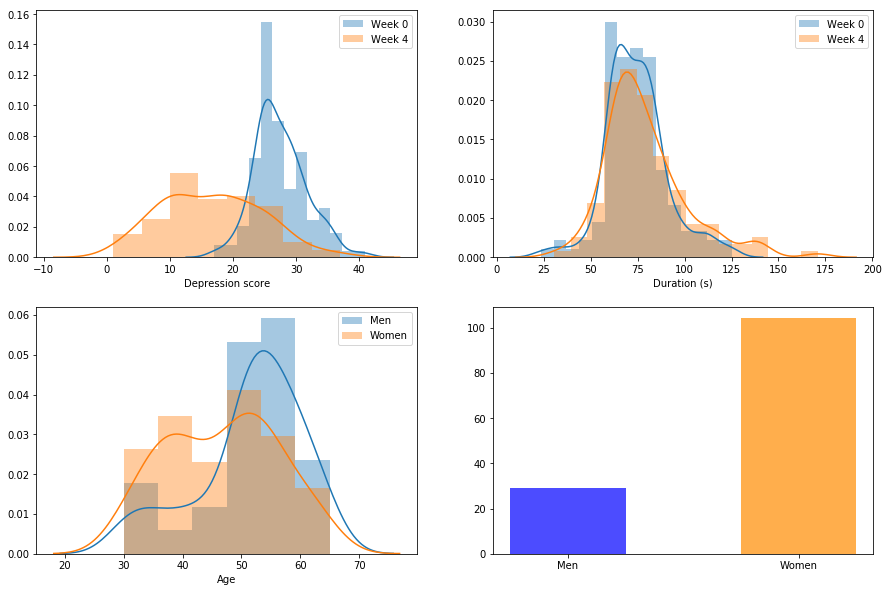
\includegraphics[width=1.0\textwidth]{./Images/dataset.png} }
  \caption[Dataset visualization.]{Visualization of the main dataset features. Starting in the upper left hand side and continuing in the clockwise direction, the first figure shows the distributions of depression scores measured on the first and second patient visit respectively. The second figure shows the distributions EEG recording durations on the first and second week respectively. The third figure shows distributions of ages for male and female participants, and the last figure visualizes the number male and female participants.}
\label{fig:dataset-viz}
\end{figure}

\begin{figure} 
\centering
\noindent\makebox[\textwidth]{%
  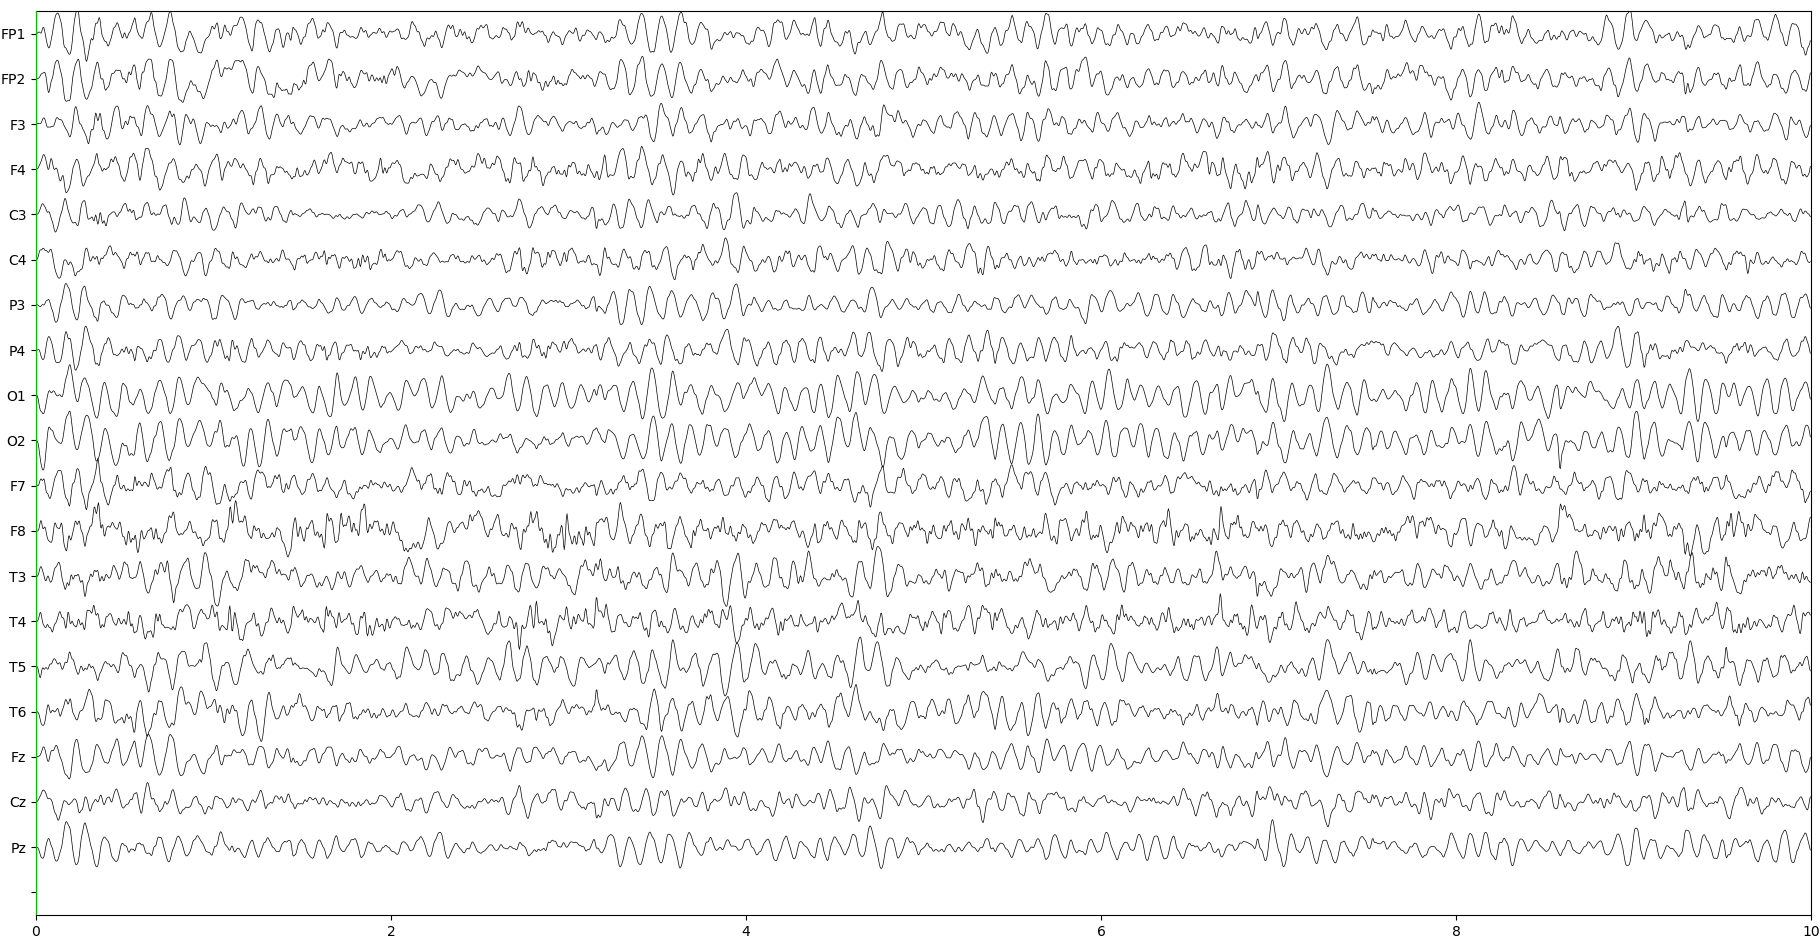
\includegraphics[width=1.0\textwidth]{Images/data.png} }
  \caption[Example EEG signal recording.]{An example recording for patient 1, first session. Horizontal line shows seconds, vertical line shows voltage scaled for purpose of visualization. }
\label{fig:data}
\end{figure}

We should recognize limitations of this dataset:
\begin{itemize}
  \item That the patients were not randomly selected - all the patients entered the study because they were experiencing problems negatively impacting their lives. Thus, as a study of depression biomarkers, the experiment lacks truly symptom absent group. However, the patients did differ significantly in severity of the disease.
  \item For a study of brain regions associated with depression, this study lacks data on patients' handedness, which may be relevant for distribution of activity in the hemispheres.
  \item For a study of response of patients to treatments, this dataset lacks a control group given no treatment (or placebo).
  \item For a study of treatment effects, patients were assigned different cominations of drugs, making an attempt of finding the singular cause of any observed effects impossible.
  \item Durations of the recordings do not allow us to put sufficiently low bound on the maximum error we can theoretically achieve for computation of the lagest Lyapunov exponent and correlation dimension (see Sections~\ref{sec:req-lyap} and~\ref{sec:req-corr}). 
\end{itemize}
\section{Preprocessing} \label{sec:nl-preprocess}
Recordings of $f_s = 1000$ Hz were downsampled (decimated) by factor $4$ to $250$ Hz using the Fourier method (also known as trigonometric interpolation), i.e. by performing discrete Fourier transform on the original series, dividing it into $2*1000/250=8$ intervals, removing all but the first and the last intervals (thus removing the highest positive and negative frequencies, corresponding to low-pass filtering), and performing inverse discrete Fourier transform. This procedure assumes that the signal is periodic, and may have some influence on the obtained results. However, it was observed that this effect is almost negligible, even for considerably higher decimation factors~\cite{diab2013effect}.

In further analysis, unless otherwise specified, recordings were shortened to fixed length of 60 s (15 000 timesteps). This measure was taken in order to achieve the the following characteristics on the data:
\begin{enumerate}
  \item minimize the stationarity effect (see Section~\ref{sec:stationarity}), and at the same time
  \item include as many timesteps in the recordings (i.e. as high time series length as possible) as possible, while
  \item including as many recordings as possible.
\end{enumerate}
This resulted in exclusion of 26 recordings from the total of 266. We have to recognize that, as we saw in Sections~\ref{sec:req-lyap} and~\ref{sec:req-corr}, this number of timesteps limits us to relatively small embedding dimensions to achieve theoretically low bounds on the maximum error for computation of multiple nonlinear measures.

In~\cite{hosseinifard2013}, band-pass filtering was used to remove frequencies which are physiologically impossible to produce by neural oscillations (e.g. high-pass filtering with 0.5 Hz threshold or lowpass filtering with 70 Hz threshold). Sometimes, it is suggested to notch filter at power line frequencies (40 Hz or 50 Hz). However, some authors suggest that linear filtering may adversely affect the results of nonlinear analysis~\cite{andreas2000}. Others, on the other hand, observed that simple linear filtering does not influence the reconstruction of embedding space considerably~\cite{Rohrbacker2009}. If quality of the data is sufficient, then filtering is not necessary~\cite{Jas2017}. 

To determine the effects of filtering on our datasets, we filtered the data to the 0.5 Hz - 70 Hz range using Butterworth filter of order 3, and then we performed the preliminary analysis described in Section~\ref{sec:distanal}. However, we did not find any significant improvement, and therefore we decided to avoid the impact of filtering on the final results.

\section{Estimation of Nonlinear Measures} \label{sec:estim-nl}
\subsection{Our Procedure}
It is well known that the results of algorithms for estimation of nonlinear measures presented in Section~\ref{sec:nonlin-meas} depend not only on the amount of noise in the data, the preprocessing and the choice of the algorithm, but also, to a considerable degree, on the embedding parameters and other input parameters~\cite{fell1994resonance, das2002applicability}. Therefore, selection of the algorithm and its parameters is of substantial importance.

Our procedure for their selection was as follows. For each nonlinear measure, we created a list of feasible parameters which we subsequentially evaluated in a preliminary analysis. Because most of the algorithms are relatively computationally expensive, length of the list should be limited. Then, we proceeded to label the data for each item on the list and evaluated it. In Section~\ref{sec:results-nl} we present the results for the most discriminative parameters. For creating the list, we used the following methods:
\begin{description}
  \item[Literature review:] Review the literature on use of the nonlinear measure in question on EEG data, and search what parameters were used. 
  \item[(Algorithm-assisted) manual estimation:] Estimate the optimal embedding parameters by analyzing the algorithm outputs for multiple samples. Use algorithms for estimating the embedding parameters and analyze their results.
  \item[Automatic pipeline:] Create automatic pipeline, which will select the optimal parameters for each sample. This step was performed only for correlation dimension and the largest Lyapunov exponent.
\end{description}

\subsection{State Space Reconstruction}
\begin{figure} 
\centering
\noindent\makebox[\textwidth]{%
  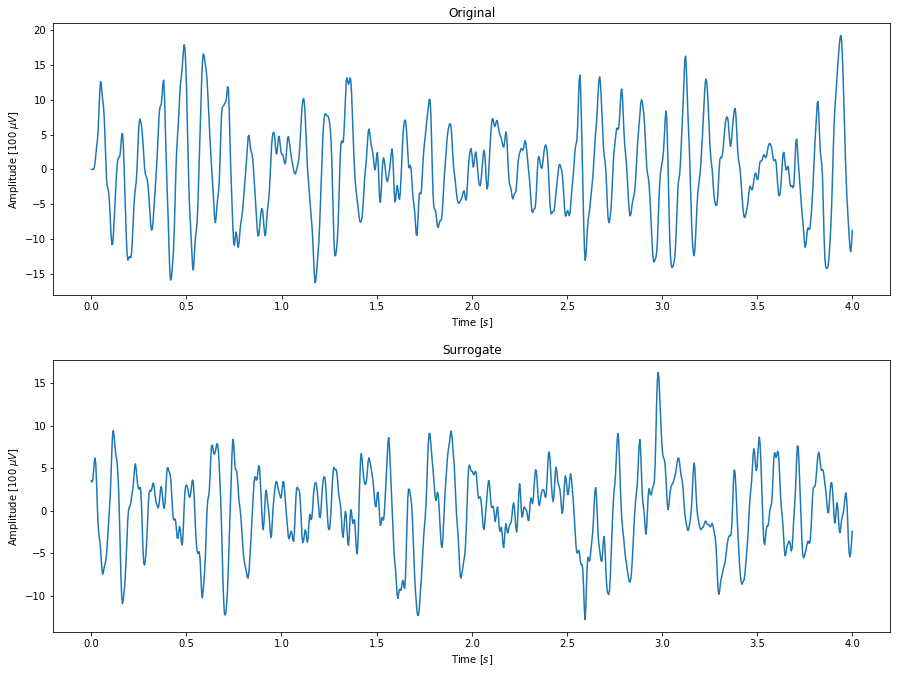
\includegraphics[width=1.0\textwidth]{Images/ts.png} }
  \caption[Comparison of a time series and its surrogate.]{A comparison of the first $4 s$ of a time series and its AAFT surrogate.}
\label{fig:ts}
\end{figure}
\subsubsection{Time Delay} \label{sec:delay-exp}
In this section, we present an analysis of the estimation of time delay using several techniques. For illustrative purposes, we explain how these techniques can be used in analysis of, and present the results of these techniques for, the signal obtained from the FP1 electrode of recording of patient 75, second visit. As described in Section~\ref{sec:dataset}, the time series, shown in Figure~\ref{fig:ts}, was clipped to 60 s (15 000 data points). The selected techniques of time delay analysis were:
\begin{enumerate}
  \item Reconstruction plots
  \item Autocorrelation $A(\tau)$ (see Section~\ref{sec:acorr})
  \item Delayed mutual information $\mathcal{I}(\tau)$ (see Section~\ref{sec:dmi})
  \item Average displacement from diagonal (ADFD) (see Section~\ref{sec:adfd})
  \item PCA reconstructions comparison (see Section~\ref{sec:svd})
  \item Integral local deformation (ILD) (see Section~\ref{sec:ild})
\end{enumerate}

Figure~\ref{fig:recon} shows reconstructed trajectories for the first 4 s (1000 data points) of the recording, for varying time delay $\tau$. As expected, the reconstructed attractors for small delays cluster along the main diagonal, expand, and then become increasingly chaotic with larger $\tau$. However, it is impossible to judge objectively on the degree of folding in the attractor from these plots (even for shorter time series), which highlights the importance of qualitative measures for EEG signals.

Typical plots of autocorrelation and delayed mutual information can be seen in Figure~\ref{fig:dmi-acorr}. First local minima of DMI and first $\tau$ for which $A(\tau) \leq 1/e$, respectively $A(\tau) \leq 1-1/e$ are marked by yellow dots. For this channel, these are $\tau_{\mathrm{DMI}} = 10$ and $\tau_{A} = 4$, respectively $\tau_{A} = 6$. It is immediately obvious that estimates of these techniques differ considerably. However, the variance of the estimated parameters is small both across channels and across patients for both techniques. To illustrate, we computed the estimates all channels of this recording, and their distribution for both DMI and autocorrelation can be seen in Figure~\ref{fig:dmi-acorr-hist}. For the selected patient, autocorrelation shows less variance and lower suggested time delays. This behavior was observed across patients.

Figure~\ref{fig:pca-svd} shows singular values of the PCA reconstruction as functions of time delay $\tau$. The two largest singular values corresponding to the main axes of the attractor clearly stand out. Besides the dominant collapse at $\tau=14$, upon closer observation, one may notice multiple smaller collapses, such as one at $\tau=7$. We can see how the attractor expands in the third and fourth dimension for $\tau=3$  (similar behavior is also visible in Figure~\ref{fig:recon}), which may suggest $\tau_{\mathrm{SVD}} \in \{3,4\}$ as optimal. However, one may also choose $\tau_{\mathrm{SVD}}=6$ as optimal, since all the attractor seems mostly unfolded in all the available directions. This highlights how subjective is evaluation of results of this technique. Thus, for automatic evaluation, it is preferrable to use other method.

The results obtained by ADFD for embedding dimensions 5, 10 and 15 can be seen in Figure~\ref{fig:adfd}; the green dashed lines represent derivatives of the respective curves, and the points mark the minimum value of $\tau$ for which derivative $\mathrm{ADFD}$ drops below $40\%$ of its initial value, as discussed in Section~\ref{sec:adfd}. The average displacement tends to increase with $m$, and saturates for relavely small values of $\tau$ - thus, the estimated time delays are (consistently) lower than those obtained by most other techniques. Moreover, ADFD requires prior selection of $m$, while the algorithms for selection of $m$ we use (FFN and AFN), require estimation of $\tau$, making this technique largely impractical.

The most powerful algorithm for embedding parameters we used is ILD. We implemented the algorithm based on Buzug's original description~\cite{buzug1992optimal}. Figure~\ref{fig:ild} shows multiple curves $\mathrm{ILD}(m,\tau)$ as functions of time delay $\tau$ for fixed values of the embedding dimension $m$. There is a clear minimum at $\tau_{\mathrm{ILD}}=4$ for all the curves, and the curves become increasingly similar. Interestingly, the convergence is slower near the minimum. Various classes of behavior were observed across channels and patients; however, since this is highly computationally expensive algorithm, it is impractical to analyze them on datasets of the size of the one used in this study.

As explained in Section~\ref{sec:delay}, these techniques should be used only as inspection tools, not as reliable guides for selection of $\tau$. The ultimate goal of the reconstruction is to obtain as accurate values of the nonlinear parameters as possible, and thus selection of the optimal embedding parameters may differ for each of them. Thus, for example, in order to select the proper embedding parameters for computation of the largest Lyapunov exponent, we inspected the scaling regions for multiple values of $m$, $\tau$, Theiler window and other parameters, and picked those with the longest scaling regions (since the length of the scaling regions is proportional to the certainty of the estimate~\cite{kennel1992determining}).

Table~\ref{tab:delay-est} shows an overview of estimated values of $\tau$. Autocorrelation, DMI, and singular values analysis report lower values than ADFD and ILD. However, Rosenstein notes that the best estimates of largest Lyapunov exponents were obtain for the autocorrelation threshold of $1-1/e$. For this threshold, the autocorrelation suggests $\tau_A = \tau_{ILD} = 4$ as optimal (and the distributions shift accordingly), thus in agreement with ILD.  

For comparison of obtained In the Section~\ref{sec:lle-exp}, we will show the effects of increasing $\tau$ on the average divergence.

\begin{table}[tbp]
\centering
\begin{tabular}{|c|c|}
\hline
\textbf{}                  & \textbf{Estimated optimal time delay} \\ \hline
Reconstruction plot        & -                                    \\ \hline
Autocorrelation            & 6, 4                                 \\ \hline
Delayed mutual information & 7                                    \\ \hline
SVD analysis               & 6                                    \\ \hline
Average displacement       & 2, 3                                 \\ \hline
Integral local deformation & 4                                    \\ \hline
\end{tabular}
\caption[Estimated optimal time delays.]{Estimated optimal time delay values of the individual examined techniques for patient 75, second session. The results vary widely based on used technique, but have relatively low variance across patients.}
\label{tab:delay-est}
\end{table}

\begin{figure} 
\centering
\noindent\makebox[\textwidth]{%
  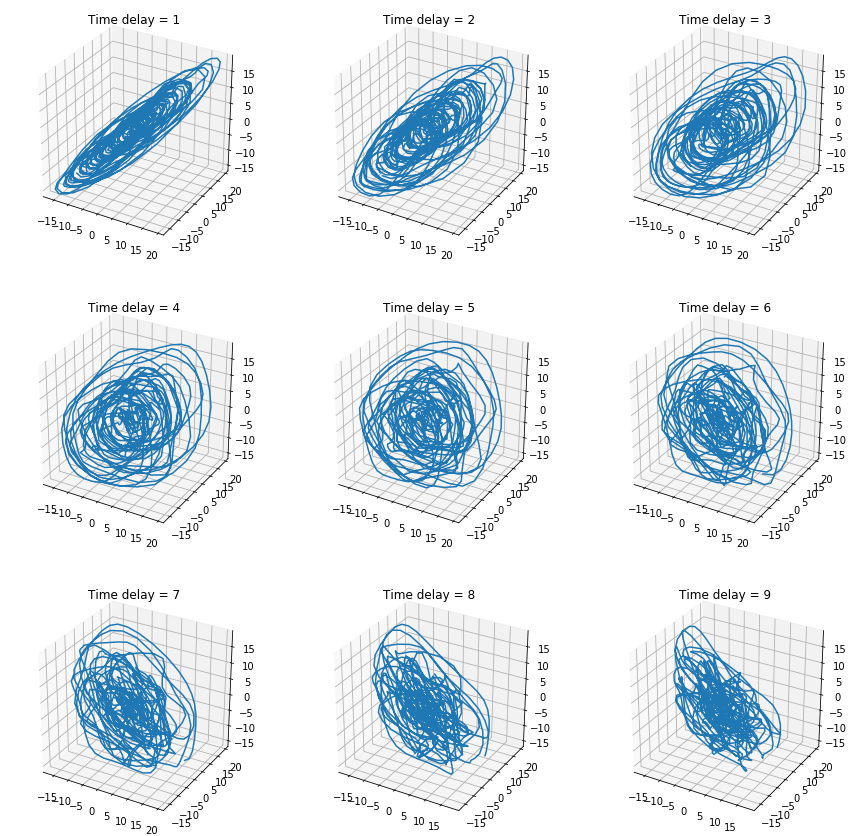
\includegraphics[width=1.0\textwidth]{Images/recon.png} }
  \caption[State space reconstructions for varying $\tau$.]{State space reconstruction for embedding dimension $m=3$ for various values of time delay $\tau$. Only first 40 seconds of the recording used for purpose of visualization. The axes represent the state vector coordinates. One may observe the increasing complexity and slowly progressing expansion of the attractor from a line to a random cloud of points. }
\label{fig:recon}
\end{figure}

\begin{figure} 
\centering
\noindent\makebox[\textwidth]{%
  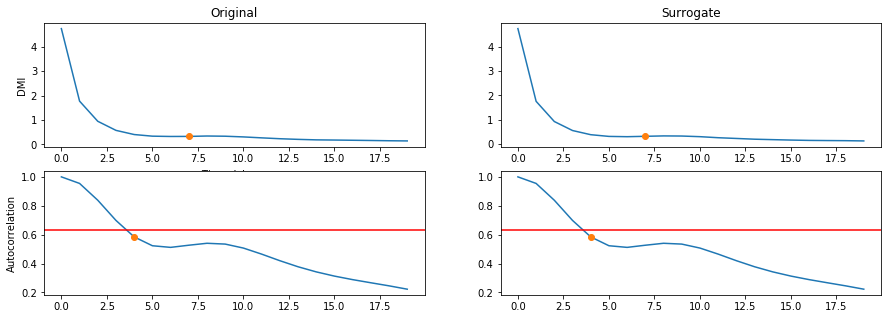
\includegraphics[width=1.0\textwidth]{Images/dmi_acorr.png} }
  \caption[DMI and $A(\tau)$ for a sample recording.]{Delayed mutual information (DMI) and autocorrelation as functions of $\tau$. The red line shows threshold values $1-1/e$ and $1/e$ respectively. The plots of surrogate data are equivalent. For this time series, DMI estimates optimal $\tau=10$, and autocorrelation $\tau=4$ or $\tau=6$. We can see that the estimates vary significantly across those techniques, but judging by Figure~\ref{fig:recon}, the autocorrelation estimates seem more reasonable.}
\label{fig:dmi-acorr}
\end{figure}

\begin{figure} 
\centering
\noindent\makebox[\textwidth]{%
  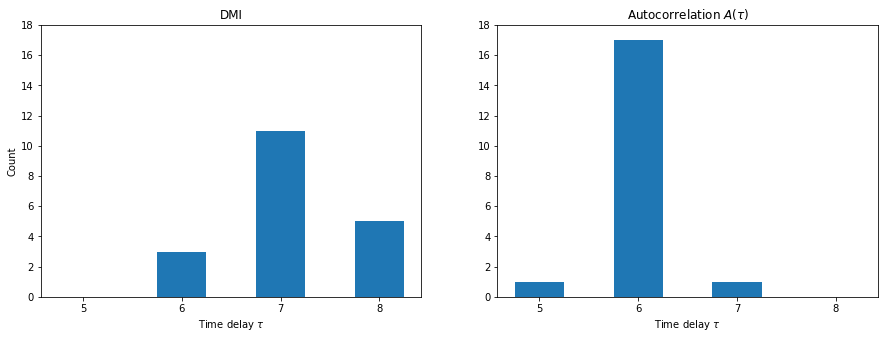
\includegraphics[width=1.0\textwidth]{Images/dmi_acorr_hist.png} }
  \caption[Distribution of $\tau$ across channels.]{Distributions of time delays across channels computed using delayed mutual information and autocorrelation for threshold $1/e$.}
\label{fig:dmi-acorr-hist}
\end{figure}

\begin{figure} 
\centering
\noindent\makebox[\textwidth]{%
  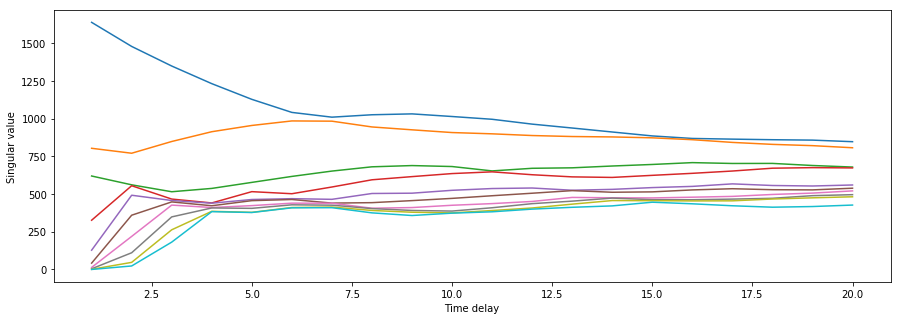
\includegraphics[width=1.0\textwidth]{Images/pca_svd.png} }
  \caption[Singular values as functions of $\tau$ for various $m$.]{Plot of singular values as functions of $\tau$ for $m=10$. The two largest singular values corresponding to the main diagonals of the attractor are clearly visible. The singular values are approximately for $\tau=12$ before a collapse in the reconstruction immediately for the following values of $\tau$.}
\label{fig:pca-svd}
\end{figure}

\begin{figure} 
\centering
\noindent\makebox[\textwidth]{%
  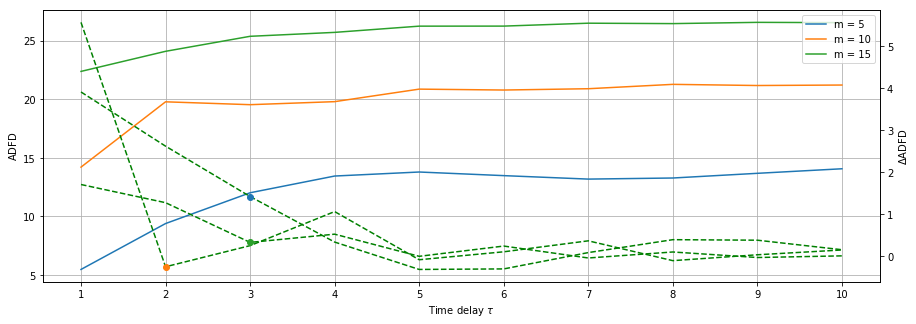
\includegraphics[width=1.0\textwidth]{Images/adfd.png} }
  \caption[ADFD as functions of $\tau$ for various $m$.]{Plot of average displacement from diagonal for embedding dimensions 5, 10, and 15. The dashed green lines represent derivatives or respectives curves, the dots mark the minimal values of $\tau$ for which the derivative of $\mathrm{ADFD}(\tau)$ reaches $40\%$ of its initial value. }
\label{fig:adfd}
\end{figure}

\begin{figure} 
\centering
\noindent\makebox[\textwidth]{%
  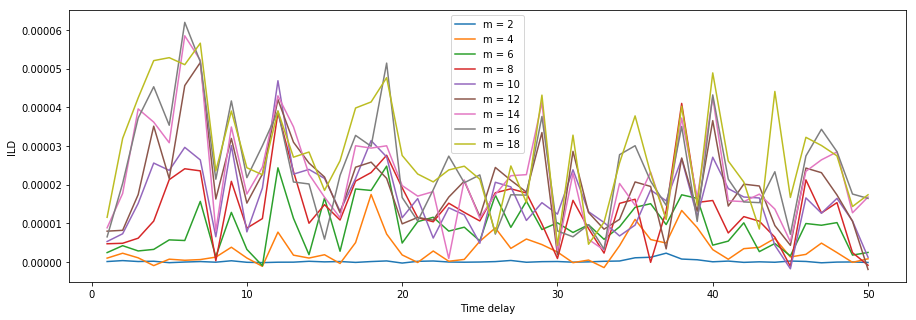
\includegraphics[width=1.0\textwidth]{Images/ild.png} }
  \caption[ILD as functions of $\tau$ for various $m$.]{Plot of integral local deformation for varying values of the embedding dimension $m$. The individual curves converge with clear minimum at $\tau=4$. The parameters used for this computation are $q_{\mathrm{max}} = 10$, $t_e = 3$, $N_{\mathrm{ref}} = N_v$, $k=20$ and $w_t = 10$ (see Section~\ref{sec:ild}).}
\label{fig:ild}
\end{figure}

\subsubsection{Embedding Dimension} \label{sec:embdim-exp}
For estimating the embedding dimension, we used combination of \emph{False Nearest Neighbors} (FNN) and Average False Neighbors (AFN) algorithms, described in Sections~\ref{sec:fnn} and~\ref{sec:afn} respectively. The convergence of ILD curves and saturation of correlation dimension also provides insight into optimal choice of embedding dimension, but, as mentioned, is impractical due to high computational cost. As explained in Section~\ref{sec:corrdim}, correlation dimension is expected to saturate for high enough choices of embedding dimension. However, we found that instead of saturating, it tended to decrease after reaching a maximum as a function of $m$, see Figure~\ref{fig:em-corrdim}. This may be because the attractor is not represented adequately in high embedding dimensions with limited amount of data. Moreover, the computational costs of this method are also considerable.

As expected, the percentage of reported false neighbors depends strongly on the selected values of $R$ and $A$ from equations (\ref{eq:first-criterion}) and (\ref{eq:second-criterion}). This is illustrated in Figure~\ref{fig:fnn-comp}, showing the percentage of false neighbors reported by the respective criteria for varying values of $A$ and $R$, and for several values of time delay $\tau$. The percentages reported by the criterion I are almost independent of $\tau$, whereas increasing $\tau$ tends to increase the percentage reported by criterion II. For high enough $\tau$, criterion II will report all neighbors as false. 

The apparent independence of the results of the criterion I on $\tau$ indicates that, regardless of $\tau$, the same percentage of near neighbors changes their distance proportionally with increase in $m$. As explained in Section~\ref{sec:fnn}, \add{Actually explain it there - nearest $\neq$ close, etc\dots,~\cite{kennel1992determining}} this behavior that can be expected of randomly generated uniformly distributed sequence of numbers. Indeed, behavior of the criterion II is consistent with this hypothesis - it eventually increases to 100\% for all values of $A$, essentially indicating infinite dimension. By selecting proper parameters and using both criteria cojointly, however, FNN can still be used to obtain reasonable results, consistent with estimates obtained by ILD, AFN, and the literature. We will use this fact in our procedure of automatic selection of embedding parameters. \add{Report average $m$ computed by ANN and FNN, $R=2.5$, $A=2.0$, $\Delta E_1 \leq 0.005$ for this patient using a histogram.}

The $E_1$ statistic of AFN usually stops increasing for approximately the same value as reported by criterion I of FNN for $R=2.5$, see Figure~\ref{fig:afn-comp}. The $E_2$ statistic, tends to oscillate in small neighborhood of value $1$, which is an indication of nondeterminism~\cite{Cao1997}.

\begin{figure} 
\centering
\noindent\makebox[\textwidth]{%
  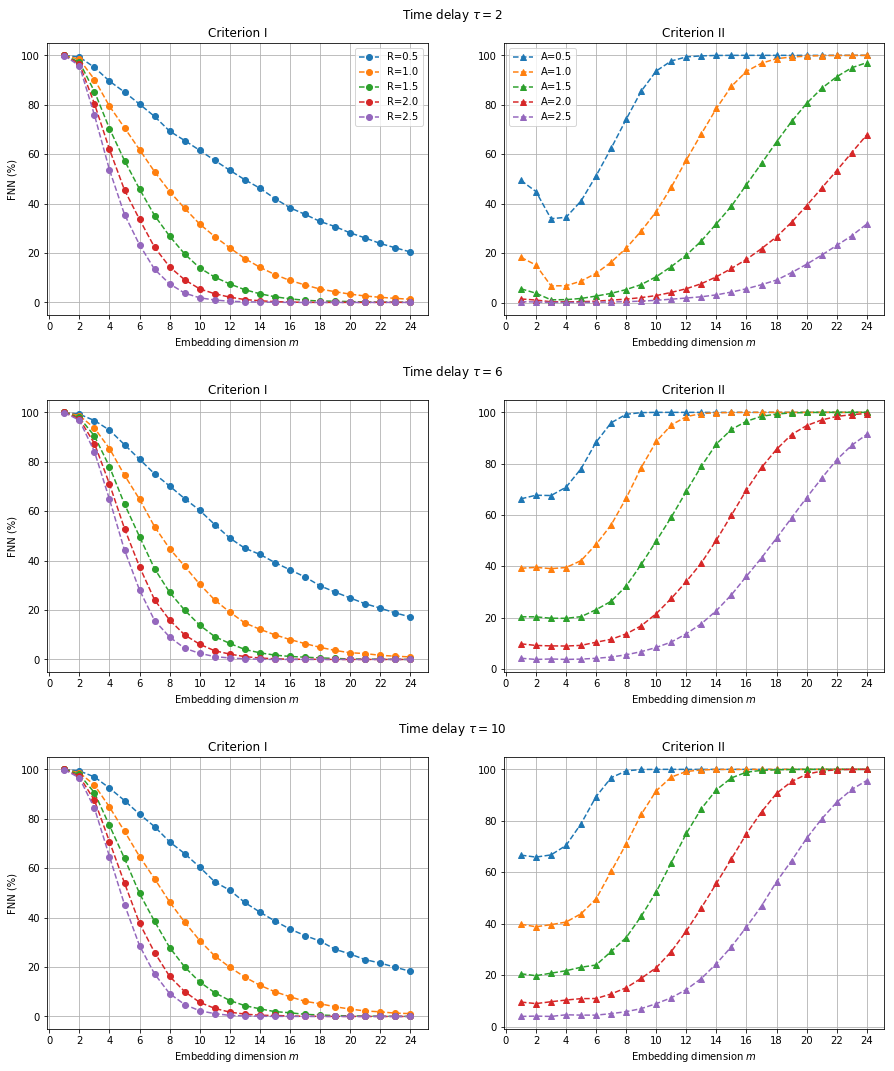
\includegraphics[width=1.0\textwidth]{Images/fnn_comp.png} }
  \caption[The effect of tolerance parameters on percentage of FNN.]{The effect of values of the tolerance parameters on the percentage of false neighbors reported by I. criterion (\ref{eq:first-criterion}) and II. criterion (\ref{eq:second-criterion}), Theiler window $w_t = 50$.}
\label{fig:fnn-comp}
\end{figure}

\begin{figure} 
\centering
\noindent\makebox[\textwidth]{%
  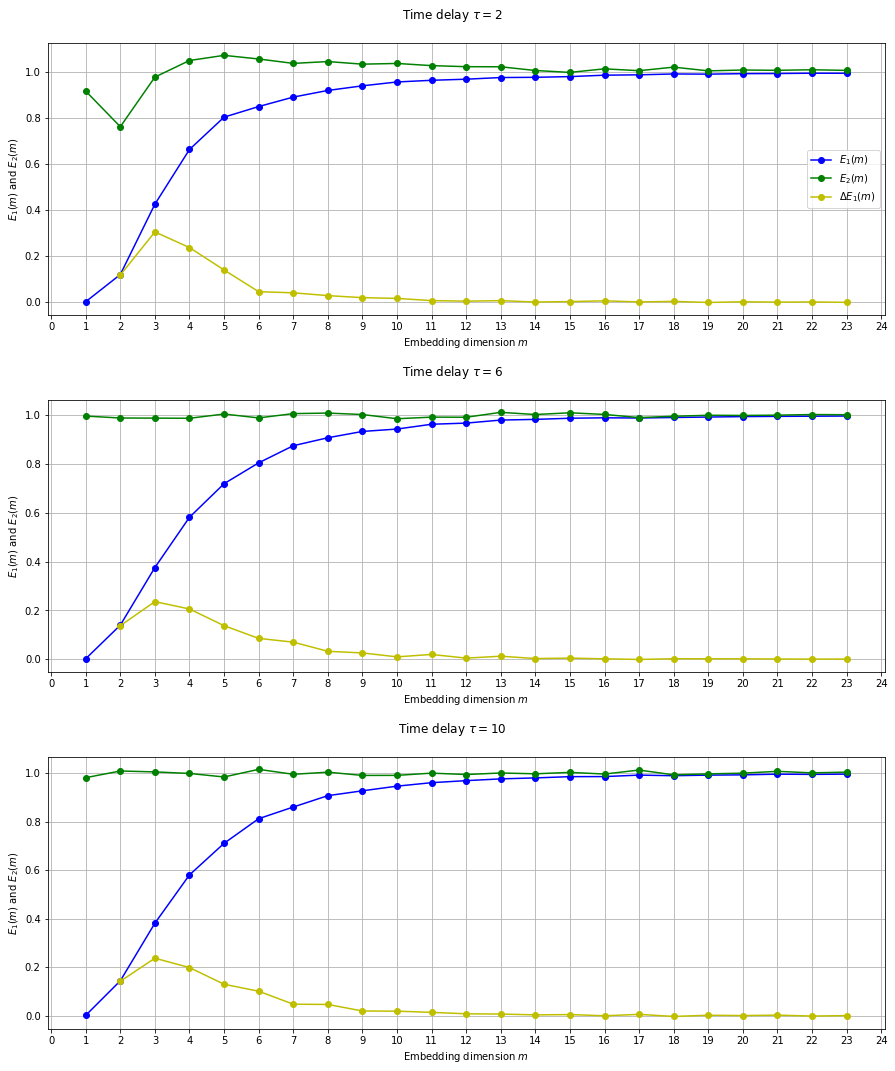
\includegraphics[width=1.0\textwidth]{Images/afn_comp.png} }
  \caption[AFN for varying values of $\tau$.]{The results of AFN for varying values of time delay $\tau$, Theiler window $w_t = 50$.  }
\label{fig:afn-comp}
\end{figure}

\subsection{Largest Lyapunov Exponents} \label{sec:lle-exp}
\subsubsection{Manual Analysis} \label{sec:lle-man-anal}
For all computations of the largest Lyapunov exponent, we used the Rosenstein's algorithm~\cite{Rosenstein1993} described in Section~\ref{sec:rosenstein}, with Theiler window $w_t$ length of 50 (200 ms). We found that the results were similar for values $w_t$ of 10, 50, 100 and 1000. Similar to Section~\ref{sec:delay-exp}, here we present an illustrative analysis of the results for the FP1 electrode of the same arbitrarily selected patient.

Figure~\ref{fig:lle-comp} shows divergence plots for different values of the embedding dimension $m$ and time delay $\tau$. Longer scaling regions correspond to higher certainty of the estimate. The short scaling regions and high slopes for small embedding dimension appear because, when the attractor is not unfolded, near neighbors are not actually close in the phase space and thus their trajectories diverge quickly. With increasing embedding dimension the scaling region clearly lengthens, but the slope also slowly approaches zero, and scaling region gradually disappears. This is because the average divergence cannot exceed the diameter of the attractor, which is finite, since the attractor is bounded in the phase space. Therefore, selecting proper embedding dimension based on divergence plots involves compromising between those two effects. Moreover, notice that the length of the scaling region is approximately $m\tau$. \unsure{How to explain this?}

With increasing time delay $\tau$, we observe gradually damped oscillation-like behavior with period $\tau$ and amplitudes also increasing with $\tau$. Average divergence we computed using Kantz' algorithm also exhibits this behavior. Oscillation-like behavior was observed for white noise data in~\cite{Rosenstein1993}, and for periodic data with period equal to the dominant period of the system in~\cite{kantz2004}. One possible explanation is as follows~\cite{fell1994resonance}. Let $x_1, x_2, \dots, x_N$ represent sampled time series, and $y_i \in \RR^{m}$ an embedded point in the reconstructed orbit. Then
\begin{align*}
  y_i               &= \begin{pmatrix} x_i & x_{i+\tau} & \dots & x_{i+(m-2)\tau} & x_{i+(m-1)\tau} \end{pmatrix} \\
  y_{i+\tau}        &= \begin{pmatrix} x_{i+\tau} & x_{i+2\tau} & \dots & x_{i+(m-1)\tau} & \mu_1 \end{pmatrix} \\
                    & \dots \\
  y_{i+(m-1)\tau}   &= \begin{pmatrix} x_{i+(m-1)\tau} & \mu_1 & \dots & \mu_{m-2} & \mu_{m-1} \end{pmatrix}. \\
\end{align*}
This means that for a given $y_i$, possible values of $y_{i+\tau}$ are restricted to a line parallel to the direction of the $m$-th basis vector. Analogously, $y_{i+2\tau}$, $y_{i+3\tau}$, \dots, $y_{i+(m-1)\tau}$ are restricted to $2, 3, \dots, m-1$ dimensional hyperplanes in the $m$ dimensional embedding space. As explained in Section~\ref{sec:rosenstein}, Rosenstein's algorithm finds pairs of vectors $y_i$ and $y_{n(i,m)}$ with certain properties, and computes the evolution of their distances over time. This means that the possible values of $y_{i+\tau}$ and $y_{n(i,m)+\tau}$ are restricted to lie on two hyperplanes parallel to the $m$-th basis vector. Therefore, if $d_i(0) = \norm{y_i - y_{n(i,m)}}$ is their initial distance, then the maximum possible distance after evolution by $\tau$ timesteps is $\norm{ y_{i+\tau} - y_{k+\tau} } = \sqrt{ (d_i(0))^2 + A_m^2 }$, where $A_m$ is the maximum amplitude $\max_{i \in N(m, \tau)}|x_i|$. However, generally, the maximum distance is $A_m \sqrt{m}$. Thus, we may expect the average distances fluctuate with period $\tau$.

There are several methods for mitigating this effect, but it cannot be evaded completely, since it is a join property of the time delay embedding and the data~\cite{fell1994resonance}. One may choose smaller $\tau$, choose the evolution time $t_e < \tau$ or $t_e \geq \tau m$. Alternatively, one may choose different time delays $\tau_i$ for individual vector coordinates. The benefit of chossing smaller time delay or bounding the evolution time is that these choices still enable using hardware acceleration provided by vectorized operations in the implementation of the algorithm. Lastly, some algorithms, such as a modification of Wolf's algorithm~\cite{roschke1995nonlineardeppression}, attempt to minimize the effect implicitly.

\unsure[inline]{Can this occur due to measurement projection? Also, even if the largest Lyapunov exponent is positive, in dissipative systems (i.e. those possessing an attractor, see Section~\ref{sec:attractor}) the sum of all Lyapunov exponents is negative, and thus, even on average, states will diverge in some directions. These effects can be compensated for by using proper averaging statistics~\cite{kantz2004}.}

\subsubsection{Automatic Selection Procedure} \label{sec:lle-auto}
To estimate the LLE values using automatic selection of proper embedding parameters, we proceeded as follows. Selection of time delay was done using autocorrelation function with threshold $1-1/e$. Results ranged from 2 to 5, depending on the channel. The selected $\tau$ was used to compute the embedding dimension with smallest FNN percentage from embedding dimensions in range from 1 to 20, i.e. $m_1 = \argmin_{m' \in \{1,\dots,20\}} \mathrm{FNN}(m')$. The tolerance parameters were $R=2.5$, $A=2.0$. Moreover, we found the first embedding dimension $m_2$ for which $E_1(m_2) - E_1(m_2-1) < 0.008$. The estimates $m_1$ and $m_2$ computed in this manner were usually similar, and ranging from 8 to 11, depending on the channel. The final embedding dimension $m$ was selected as their average $m = \ceil{m_1 + m_2)/2}$. The length of the scaling region $t_e = m\tau$ and the Theiler window, as mentioned, $w_t = 50$.

\begin{figure} 
\centering
\noindent\makebox[\textwidth]{%
  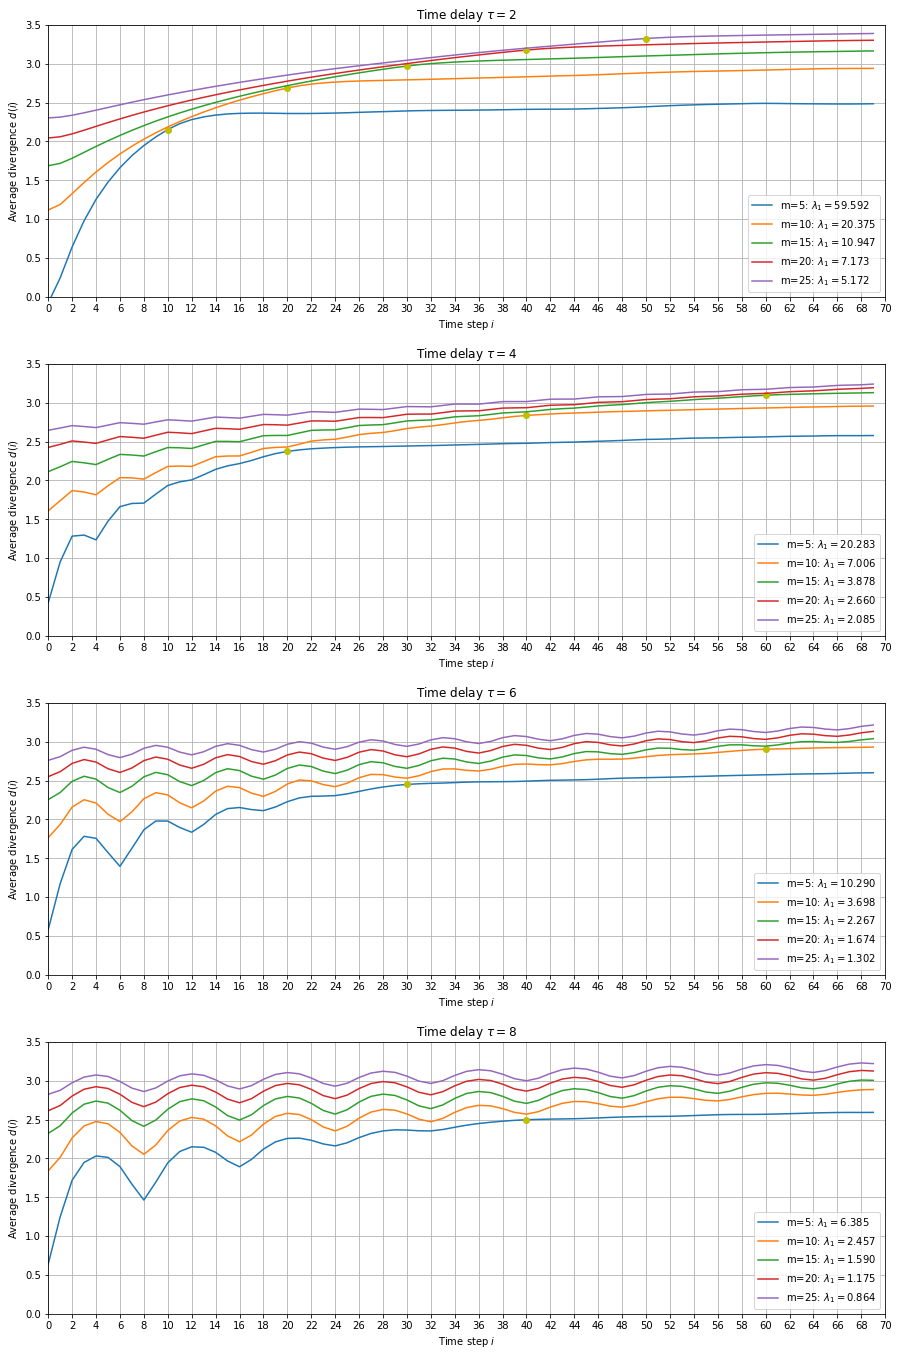
\includegraphics[width=0.9\textwidth]{Images/lle_comp.png} }
  \caption[Effects of embedding parameters on average divergence plots.]{Average divergence plots for varying values of $m$ and $\tau$.}
\label{fig:lle-comp}
\end{figure}

\subsubsection{Literature Review} \label{sec:lle-rev}
Using the correlation dimension saturation, the following estimates have been obtained: 5~\cite{babloyantz1986low}, 7~\cite{blanco1995stationarity}, 6-8 (depending on sleep stage)~\cite{gallez1991predictability}. We found similar estimates using correlation dimension maximum (as mentioned in Section~\ref{sec:embdim-exp}, we observed no saturation) with time delay $\tau=1$.

By analyzing records ECT seizures, manually separating them into more and less regular, and inspecting multiple values of LLE as a measure of separation between these classes, 7 was selected as optimal embedding dimension in~\cite{krystal1997largest}.

Remaining studies we evaluated, including some analyzing depression, used embedding dimension 10~\cite{roschke1995nonlineardeppression, fell1993deterministic, roschke1993calculation}. Especially relevant is~\cite{roschke1995nonlineardeppression}, where depression data were analyzed, including the dependence of LLE on the embedding dimension. The authors decided to use various values of time delay depending on the embedding dimension corrdinate (for rationale, see Section~\ref{sec:lle-man-anal}). Emotion recognition using LLE from EEG signals was performed in~\cite{aftanas1997non} with embedding dimension $m=10$ and time delay $\tau=3$. No reasoning behind this choice was provided. Summary of the reviewed studies can be seen in Table~\ref{tab:litrev-lle}.

\begin{table}[tbp]
\resizebox{\textwidth}{!}{
\begin{tabular}{|c|c|c|c|c|}
\hline
$\mathbf{m}$ & \textbf{Method of selection of m} & $\mathbf{\tau}$ & \textbf{Application} & \textbf{Reference} \\ \hline
5 & $D_2$ saturation & - & epileptic seizures & ~\cite{babloyantz1986low} \\ \hline
7 & $D_2$ saturation & 5 & stationarity estimation &~\cite{blanco1995stationarity}  \\ \hline
6-8 & $D_2$ saturation & DMI & measuring variance in $D_2$ during sleep &~\cite{gallez1991predictability} \\ \hline
7 & - & 10 & measuring regularity during ECT seizures &~\cite{krystal1997largest} \\ \hline
10 & - & 3 & emotion recognition &~\cite{aftanas1997non}  \\ \hline
10 & - & zero-crossing of $A(\tau)$ & sleep in schizophrenia &~\cite{roschke1995nonlinearschizo} \\ \hline
10 & - & zero-crossing of $A(\tau)$ & sleep &~\cite{fell1993deterministic} \\ \hline
10 & - & random & depression &~\cite{roschke1995nonlineardeppression} \\ \hhline{=|=|=|=|=}
10 & - & 3 & depression & - \\ \hline
11-15 & FNN, AFN average & $1-1/e$ crossing of $A(\tau)$ & depression & - \\ \hline
\end{tabular}}
\caption[Literature review of LLE embedding parameters.]{Embedding dimension $m$ and time delay $\tau$ choices found across available literature, along with methods of their selection and particular use case. All the studies used sampling frequency in range $250-256$ Hz. The range results we obtained using various algorithms and observed in literature highlights the fact that the embedding parameters selection algorithms, as well as visual inspection of the divergence plots largely are unreliable, and that the optimal values depend on particular dataset and problem.}
\label{tab:litrev-lle}
\end{table}

In summary, we obtained a wide range of results using traditional parameter selection techniques, with the most powerful algorithm, ILD, indicating sligthly lower values of time delay. Most of the embedding dimension estimation algorithms, including ILD, agree with the literature that the optimal embedding embedding dimension should be set around 10. We proceeded with computing multiple sets of LLE labels for the dataset, each with a different member of the following set of input parameters $(m, \tau)$: $(7, 3)$, $(7,6)$, $(10,3)$, $(10, 6)$, $(15, 4)$, automatic (as described in Section~\ref{sec:lle-auto}). Then, we analyzed the label distributions between studied groups, as presented in Section~\ref{sec:distanal}, where we present results only for the most discriminative pairs of parameters, which was $m=10$, $\tau=3$.

\subsection{Correlation Dimension} \label{sec:corrdim-exp}
\subsubsection{Manual Analysis} \label{sec:corrdim-anal}
For computation of correlation dimension, we used Grassberger-Procaccia algorithm described in Section~\ref{sec:corrdim}, using Chebyshev metric (as suggested in~\cite{andreas2000}), Theiler window $w_t = 50$, for values of $r$ either in geometrical progression of 100 values from 0.05 to 10. Hereby we analyze the results for patient number 75, second session, FP1 electrode.

Plots of normalized correlation sums $C(r)$ as functions of radius $r$ (both axis are logarithmically scaled) for embedding dimensions $m=5,7,11, \dots, 29$ can be seen in Figure~\ref{fig:cr}. Different time delay $\tau$ has been used for each plot. The reader may want to compare these results with Figure~\ref{fig:exp-cr}. There are clear straight lines indicating expected relationship $C(r) \propto r^{D_2}$. Also, as expected, we can see that the lines shift to the right, increasing their slopes with $m$. The effect of time delay is noticeably weaker than in LLE estimation.

Figure~\ref{fig:loc-d2} shows the local slope of $\log C(r)$ as a function of $r$ (axis logarithmically scaled). The local slope has been approximated for each value of $r_i$ by considering its 6 neighbors $\log r_{i-3}$, $\log r_{i+3}$, and fitting a line through the seven points $(\log r_{i-3}, \log C(r_{i-3})), \dots,(\log r_{i+3}, \log C(r_{i+3})$ and minimizing least squares error. In contrast with the ideal case presented in Figure~\ref{fig:exp-localcr}, there are no apparent scaling regions at all, which means we cannot provide theoretically meaningful finite estimate of $D_2$ using this method. Morever, by comparing with the same plot for iAAFT surrogate of the same time series (see Figure~\ref{fig:loc-d2-comp}), we cannot even reject the hypothesis of a linear stochastic process. These results are not unique for this sample - we obtained similar results for all other examined samples.

On the other hand, as explained in Section~\ref{sec:surrogate-analysis-theory}, even rejecting the null hypothesis is not a sufficient proof of nonlinearity. In addition, this effect is known to happen due to noise, and many studies have failed to significantly distinguish EEG data from surrogates~\cite{andreas2000}. 

\begin{figure} 
\centering
\noindent\makebox[\textwidth]{%
  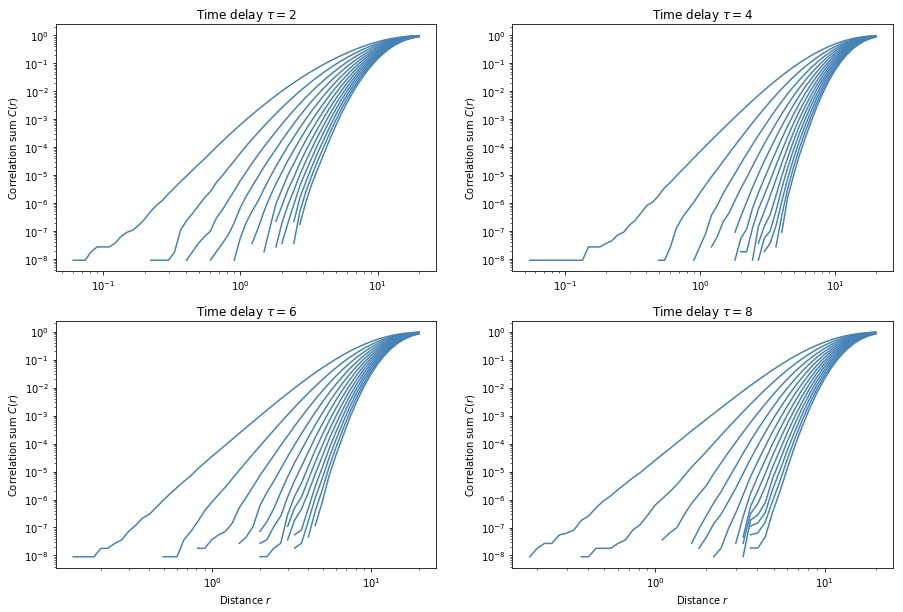
\includegraphics[width=1.0\textwidth]{Images/cr.png} }
  \caption[Normalized $C(r)$ for various $m$.]{Normalized correlation sum $C(r)$ as a function of radius $r$ for embedding dimensions $m=5, 7, 9, \dots, 29$ (lowest $m$ at the bottom, highest at the top) and time delays $\tau=2,4,6,8$.}
  \label{fig:cr}
\end{figure}

\begin{figure} 
\centering
\noindent\makebox[\textwidth]{%
  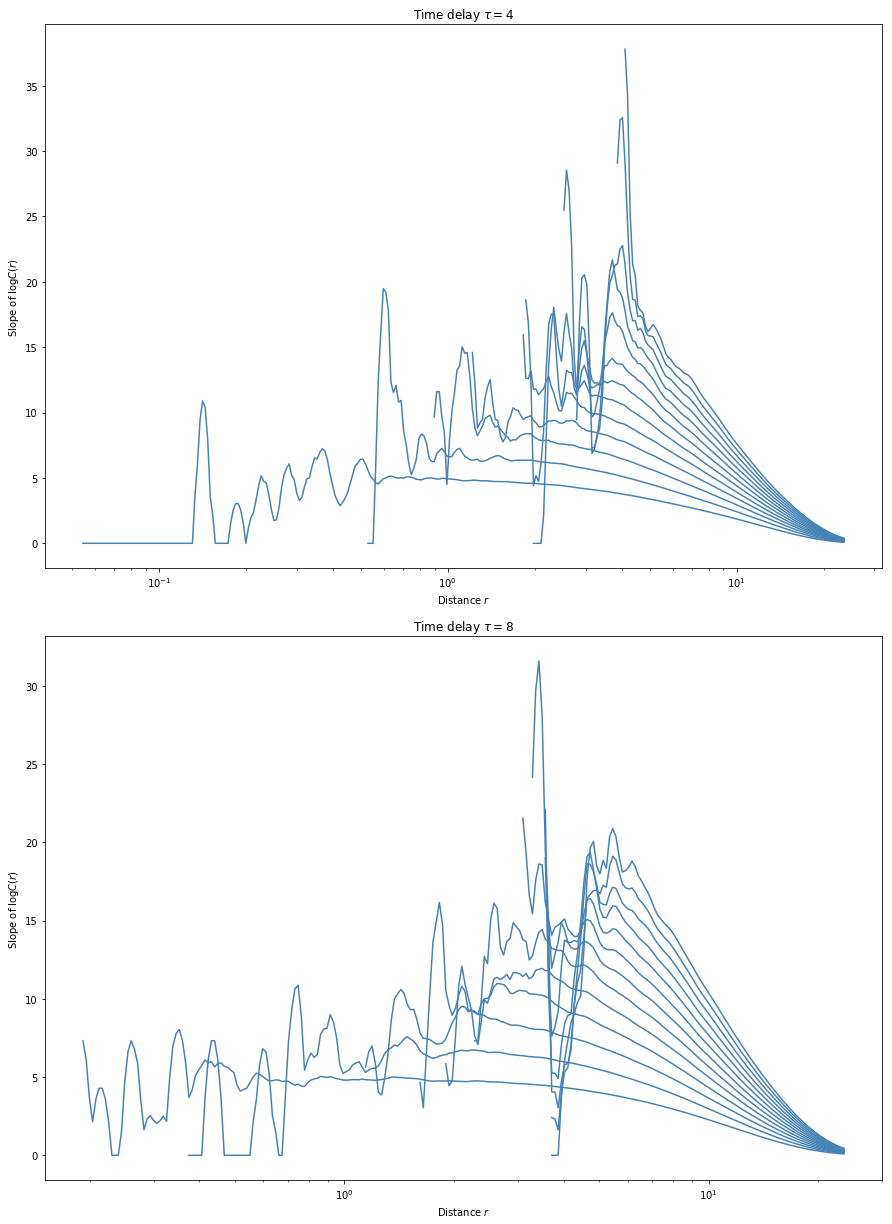
\includegraphics[width=0.95\textwidth]{./Images/local_d_2/large.png} }
  \caption[Local $D_2(r)$ for various $m$.]{Local correlation dimension $D_2$ as a function of radius $r$ for embedding dimensions $m=5, 7, 9, \dots, 29$ (lowest $m$ at the bottom, highest at the top) and time delays $\tau = 4$ and $\tau = 8$.}
  \label{fig:loc-d2}
\end{figure}

\begin{figure} 
\centering
\noindent\makebox[\textwidth]{%
  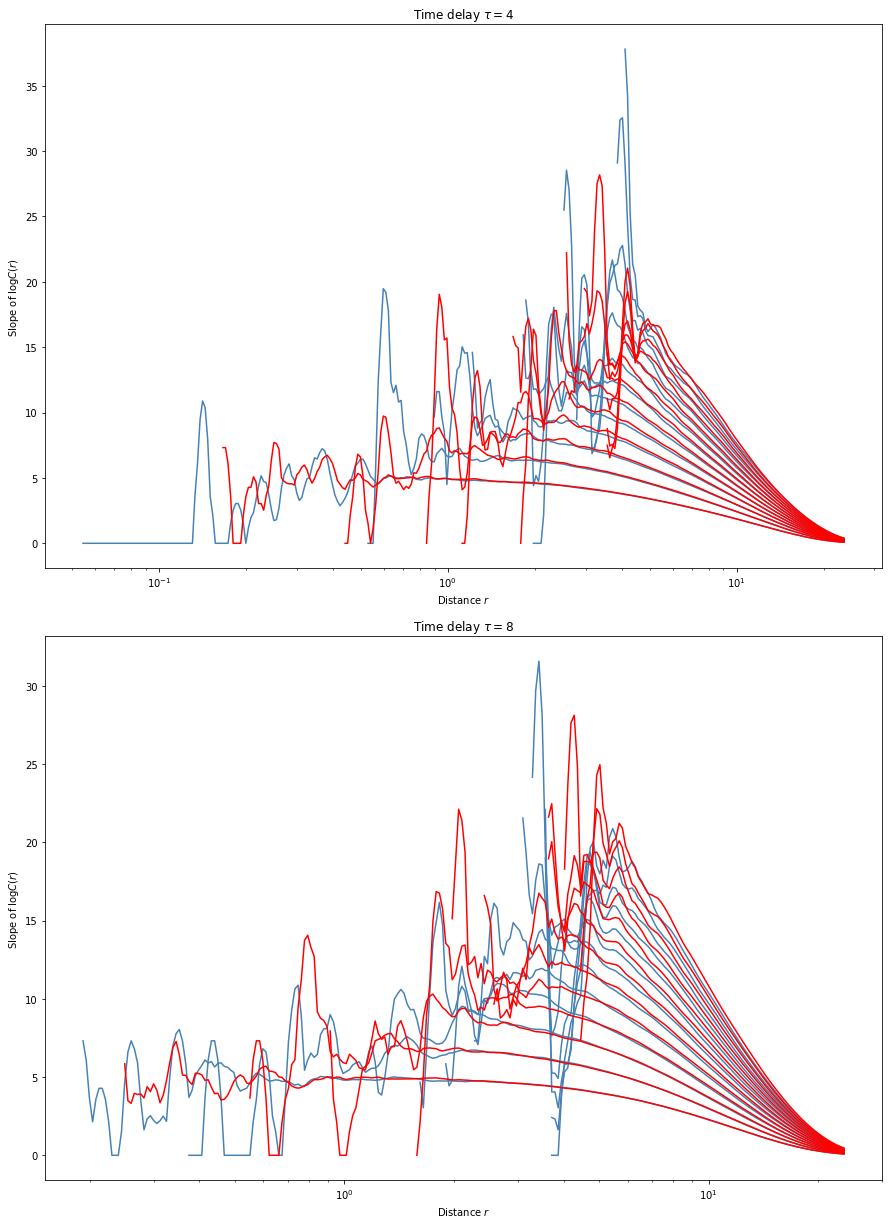
\includegraphics[width=0.95\textwidth]{./Images/local_d_2/large_surr.png} }
  \caption[Local $D_2(r)$ for various $m$ in comparison with a surrogate.]{Local correlation dimension $D_2$ as a function of radius $r$ for embedding dimensions $m=5, 7, 9, \dots, 29$ (lowest $m$ at the bottom, highest at the top) and time delays $\tau = 4$ and $\tau = 8$ for the original series (blue) and its surrogate series computed using iAAFT (red).}
  \label{fig:loc-d2-comp}
\end{figure}

\subsubsection{Automatic Selection Procedure}
To compute correlation dimension automatically, we proceeded as follows. We create multiple embeddings with incresing embedding dimensions in range from 2 to 30 with the optimal time lag selected according to the autocorrelation function with threshold $1-1/e$. For each embedding, we evaluate the slope of $\log C(\log r)$ on the interval $[r_{\mathrm{lower}}, r_{\mathrm{upper}}]$, where $r_{\mathrm{lower}}$ corresponds to the average nearest neighbor distance on the reconstructed attractor, $r_{\mathrm{upper}}$ is given by
\begin{align*}
  \log r_{\mathrm{upper}} = \log r_{\mathrm{lower}} + \frac{1}{10} \left( \log r_{\mathrm{max}} - \log r_{\mathrm{lower}} \right), 
\end{align*}
where $r_{\mathrm{max}}$ denotes the largest ocurring pairwise distance on the attractor. This approach of automatic selection radius bounds for evaluation of $D_2$ is borrowed from~\cite{andreas2000}. Then, we computed the slope of the correlation integral $C(r)$ over this scaling region for each of those embeddings using the method explained in previous section, and select the global maximum as the final value.

Figure~\ref{fig:em-corrdim} shows $D_2$ computed this way as a function of the embedding dimension $m$ for varying values of the embedding dimension $\tau$. There are no signs of saturation, correlation dimension reaches a global maximum and then starts to decrease. This may be because of insufficient data. The reached maximum value of $D_2$, however, is reasonably consistent with results obtained by various methods in the literature~\cite{pereda1998non, dvorak1986some, koukkou1993dimensional}.

\begin{figure} 
\centering
\noindent\makebox[\textwidth]{%
  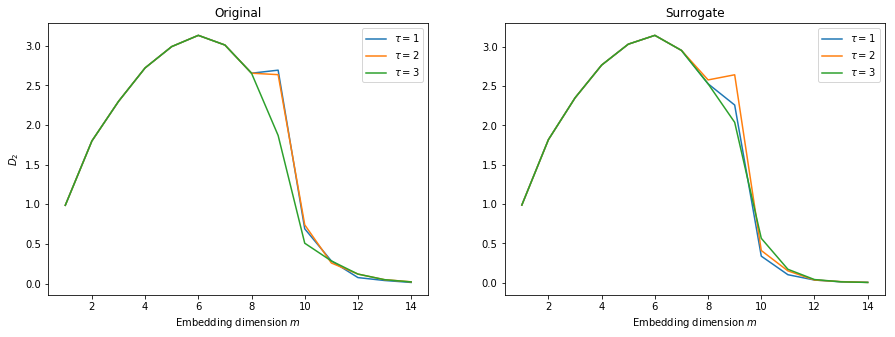
\includegraphics[width=1.0\textwidth]{./Images/em_corrdim.png} }
  \caption[Global $D_2$ as function of $m$.]{Correlation dimension as function of the embedding dimension $m$.}
\label{fig:em-corrdim}
\end{figure}

\subsubsection{Literature Review} \label{sec:corrdim-rev}
\begin{table}[tbp]
\resizebox{\textwidth}{!}{
\begin{tabular}{|c|c|c|c|c|}
\hline
$\mathbf{m}$ & \textbf{Method of selection of m} & $\mathbf{\tau}$ & \textbf{Application} & \textbf{Reference} \\ \hline
3-30 & saturation & DMI & depression &~\cite{hosseinifard2013} \\ \hline
 - &  ``unfolding dimension'' (see text) & objective function minimization & intraindividual classification &~\cite{schmid1996indications} \\ \hline
 2-20 (scaling region 16-20) & saturation & $A(\tau)$, threshold $1/e$ & awake / sleep classification &~\cite{pereda1998non} \\ \hline
 12 & - & 8 & mental state classification &~\cite{dvorak1986some} \\ \hline
 2-12 & saturation & 5 & schizophrenia &~\cite{koukkou1993dimensional} \\ \hhline{=|=|=|=|=}
 15 & - & 4 & depression & - \\ \hline
 2-30 & saturation & $1-1/e$ crossing of $A(\tau)$ & depression & - \\ \hline
\end{tabular}}
\caption[Literature review of CD embedding parameters.]{Embedding dimension $m$ and time delay $\tau$ choices found across available literature, along with methods of their selection and particular use case. All the studies used sampling frequency in range 200-256 Hz.}
\label{tab:litrev-cd}
\end{table}

In~\cite{schmid1996indications}, the authors layed out fully automatic, albeit complicated, algorithm for selecting the embedding parameters. They suggest modelling correlation dimension biparametrically as a function of embedding dimension $m$ as $D_2(m) = b_0(1-e^{-b_1m})$, where $b_0$, $b_1$ are parameters. They call $m^* \coloneqq 1/b_1$ the unfolding dimension, since ``it represents the embedding dimension at which the attractor has unfolded up to $1/e$ of its full extent, namely, the asymptotic $D_2$ value: $b_0$''~\cite{schmid1996indications}. The optimal embedding dimension $m$ is selected as the next integer greater than the embedding dimension at which the exponential fit has approached 95\% of its expontial value $b_0$. The remaining studies used either threshold crossing of the autocorrelation function $A(\tau)$ or fixed value for selection of time delay $\tau$. Although~\cite{pereda1998non} used $1/e$ as the threshold for the autocorrelation function, we found that the threshold $1-1/e$ results in better discrimination between studied groups using correlation dimension.

% Most of the studies where $D_2$ has been estimated from an EEG signal omit the step of searching of the optimal scaling region. Indeed, as reviewed in~\cite{andreas2000}, 

In summary, our experiments show lack of scaling regions in local $D_2$, indicating that no theoretically meaningful interpretation of correlation dimension is possible. Similar behavior is observed in surrogate data, hence even the null hypothesis of a linear stochatic process cannot be rejected. Moreover, our automatic procedure fails to saturate - however, this may be due to limited amount of data. Many studies reviewed in~\cite{andreas2000} failed to reveal finite embedding dimension on EEG data using the local slopes approach. The studies we examined all omitted the step of searching for optimal scaling region, and still succeeded in using $D_2$ for classification, simply by fitting the $C(r)$ curve. Table~\ref{tab:litrev-cd} shows a summary of of the studies we examined.

For these reasons, we decided to use the same approach (in addition to our automatic approach). We selected fixed pairs out of all combinations of the following values of $m=10, 15, 20, 25$ and $\tau=4, 8$ and computed correlation dimension for each sample with each pairs of embedding parameters by fitting the $\log C(r)$ against $\log r$ curve with a line using least squares fo values of $r$ geometrically progressing from $0.05$ to $10$. The most discriminative pairs of parameters were $m=15$, $\tau=4$, in accordance with our ILD algorithm. Moreover, we also computed correlation dimension for each sample using our automatic approach described above. For both, we used Theiler window $w_t = 50$.

Another approach we evaluated, following the suggestion in~\cite{andreas2000}, is to cut each sample into a number of small (overlapping) ``moving windows'', and perform the steps of estimating embedding parameters and computing correlation dimension for each of those windows. As we noted in~\ref{sec:req-corr}, increasing the time series length is theoretically assumed to improve the estimates. On the other hand, shortening the time series may ameliorate the issue of apparent non-stationarity of EEG signal we observed in Section~\ref{sec:corrdim-anal}, since for a short time intervals, the signal may be assumed approximately nonstationary~\cite{andreas2000}.

\subsection{Detrended Fluctuation Analysis} \label{sec:dfa-exp}
The concept of Detrended Fluctuation Analysis (DFA) was described in Section~\ref{sec:dfa-theory}. To compute it, we used the method of fitting a scaling region on curve of log-fluctuations $\log F(n)$ against logorarithm of segment lengths $\log n$ (see (\ref{eq:dfa-fm})), as explained in Section~\ref{sec:dfa-theory}. Following the suggestions in~\cite{hardstone2012detrended}, we defined the set of segment lengths $n$ to be spread equidistantly on a logarithmic scale (by multiplying by factor 1.1), with the lower bound of $4$ (fitting a line through less points may be prone to error). The upper bound was gradually increased, until a scaling region appeared on the curve of $\log F(n)$ against $\log n$ (see Figure~\ref{fig:dfa-fit}). This curve was then plotted across multiple channels and patients, to determine the interval where the scaling region usually appeared, and if an automatic procedure for finding a scaling region is necessary. However, the interval was approximately same for all samples, and appear for values of $n\in(50, 320)$.

\begin{figure} 
\centering
\noindent\makebox[\textwidth]{%
  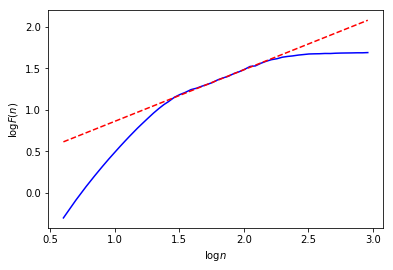
\includegraphics[width=\textwidth]{./Images/dfa_fit.png} }
  \caption[Computation of DFA.]{These figures show logarithm of root mean squared errors $\log F(n)$ (see equation (\ref{eq:dfa-fm})) plotted against logarithm of the segment length $n$. On the left hand side, each curve corresponds to one electrode for patient 75, second session. We can observe clear common scaling region for values of $n\in(50, 320)$. On the right hand side, an example regression line fitted to the scaling region of one curve is shown.}
\label{fig:dfa-fit}
\end{figure}

Moreover, following the suggestions in~\cite{hardstone2012detrended}, we evaluated DFA computed from the envelope of the signal band-pass filtered to each one of alpha (8-13 Hz), beta (16-37 Hz), and theta (4-7 Hz) frequencies, which were all found to be associated with depression~\cite{lee2007detrended, bachmann2013, linkenkaer2005breakdown}. The bounds of the scaling region were modified using the method above to $r \in (4, 100)$. However, for DFA estimates obtained using this method, we obtained no significant differences between the studied groups using the tests performed in Section~\ref{sec:distanal}.
\subsection{Hurst Exponent} \label{sec:hurst-exp}
Hurst Exponent (HE) was described in Section~\ref{sec:dfa-theory}. As far as we know, the literature regarding HE estimation omits description of the chosen values $n$ for which to calculate the scaled range $(R/S)_n$. However, we may expect that higher values of subinterval lengths $n$ will result in smaller number of subsequences $d$, and thus less precise estimate of the mean $(R/S)_n$ in (\ref{eq:hurst-mean}). This effect will also be increasingly pronounced with decreasing original time series length $N$. Indeed, in Figure~\ref{fig:hurst-fit}, which shows the mean rescaled ranges $(R/S)_n$ as a function of the subsequence length $n$ (both axes are logarithmically scaled) for all electrodes, we may observe larger fluctuations for larger values of $n$, likely because of increasing uncertainty due to this effect. It has been observed that small values of $n$ also lead to large deviations from the linear slope~\cite{weron2002estimating}, because the relationship (\ref{eq:resc-range}) is asymptotic, and thus valid only for large $n$. Nonetheless, in our case, we have not encountered this phenomenon. Therefore, we have decided to compute the Hurst exponent as the slope of the log $R/S$ curve for the values if $n\in(0,20)$ spaced equidistantly on the logarithmic scale.

\begin{figure} 
\centering
\noindent\makebox[\textwidth]{%
  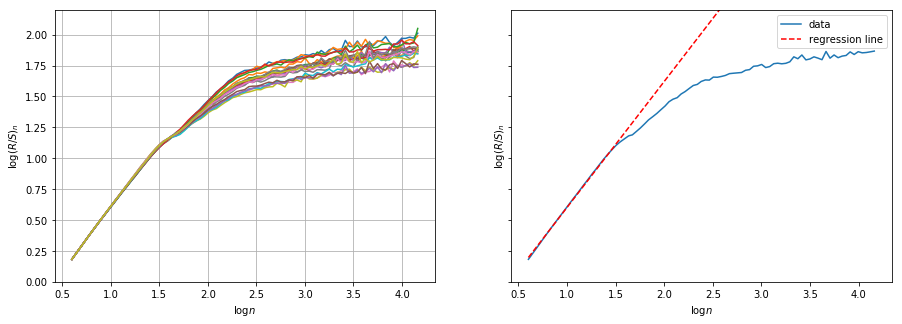
\includegraphics[width=\textwidth]{./Images/hurst_fit.png} }
  \caption[Computation of HE.]{These figures show logarithm of the scaled range (see equation (\ref{eq:hurst-rs})) plotted against logarithm of the segment length $n$. On the left hand side, each curve corresponds to one electrode for patient 75, second session. We can observe clear common scaling region for values of $n\in(0, 20)$. On the right hand side, an example regression line fitted to the scaling region of one curve is shown.}
\label{fig:hurst-fit}
\end{figure}

\subsection{Higuchi's Fractal Dimension} \label{sec:hd-exp}
\begin{figure} 
\centering
\noindent\makebox[\textwidth]{%
  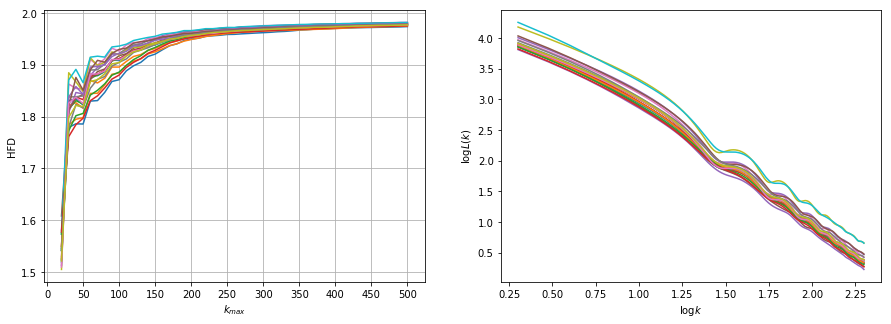
\includegraphics[width=\textwidth]{./Images/hfd_anal.png} }
  \caption[Dependance of HD on $k_{\mathrm{max}}$ parameter.]{Figure on the left hand side shows values of Higuchi's fractal dimension as a function of $k_{\mathrm{max}}$ parameter for all channels of patient number 75, second session. We can see that HD values plateau for $k_{\mathrm{max}} > 200$ for all channels. On the other hand, variance among channels disappears. Figure on the right hand side shows logarithm of mean curve length $L(k)$ as a function of $\log k$. There is a clear linear trend with slight fluctuations for higher values of $k$.}
\label{fig:hd-anal}
\end{figure}
The algorithm for estimating Higuchi's fractal Dimension (HD), as described Section~\ref{sec:hd-theory}, requires selecting the values $k$ for which $L(k)$ is to be computed. Since this can be done relatively fast, we do this by selecting values equidistant on logarithmic scale $k_1, k_2, \dots, k_{\mathrm{max}}$, where $k_{\mathrm{max}}$ is the single input parameter. Indeed, by using this approach, we follow most of the studies we evaluated.

It has been suggested that the parameter $k_{\mathrm{max}}$ can be selected by plotting values of HD as a function of $k_{\mathrm{max}}$, and selecting the value of $k_{\mathrm{max}}$ where the values of HD plateau. Our results can be seen in Figure~\ref{fig:hd-anal}. 

In~\cite{bachmann2013}, the authors computed HD for each patient as follows. They used 5 second sliding windows with 0.5 second shift and computed local HD for each of those windows using $k_{\mathrm{max}}=50$, thus obtaining 591 values per recording. The final HD for each electrode was obtained by averaging all local HDs. We tried using the same approach. However, the labels obtained in this way were less discriminative in our study. Finally, we computed labels from the entire recording for values $k_{\mathrm{max}}=7, 30, 50, 100, 200$, where $k_{\mathrm{max}}=50$ was shown to be the most discriminative.

\add[inline]{Maybe few more studies.}

\begin{table}[tbp]
  \centering
\begin{tabular}{|c|c|c|c|c|}
\hline
$\mathbf{k_{\mathrm{max}}}$ & \textbf{Sampling Frequency} (Hz) & \textbf{Recording Time} & \textbf{Application} & \textbf{Reference} \\ \hline
30 & 256 & 5 min & depression &~\cite{hosseinifard2013} \\ \hline
50 & 256 & 5 s & depression &~\cite{bachmann2013} \\ \hline
48 & 169.55 & 5 min & depression &~\cite{gomez2009use} \\ \hline
\end{tabular}
\caption[Literature review of choice for HD $k_{\mathrm{max}}$ parameter.]{Summary of choices for the $k_{\mathrm{max}}$ parameter for Higuchi's fractal dimension applied to EEG we found across literature.}
\end{table}

\subsection{Sample Entropy} \label{sec:se-exp}
\begin{figure} 
\centering
\noindent\makebox[\textwidth]{%
  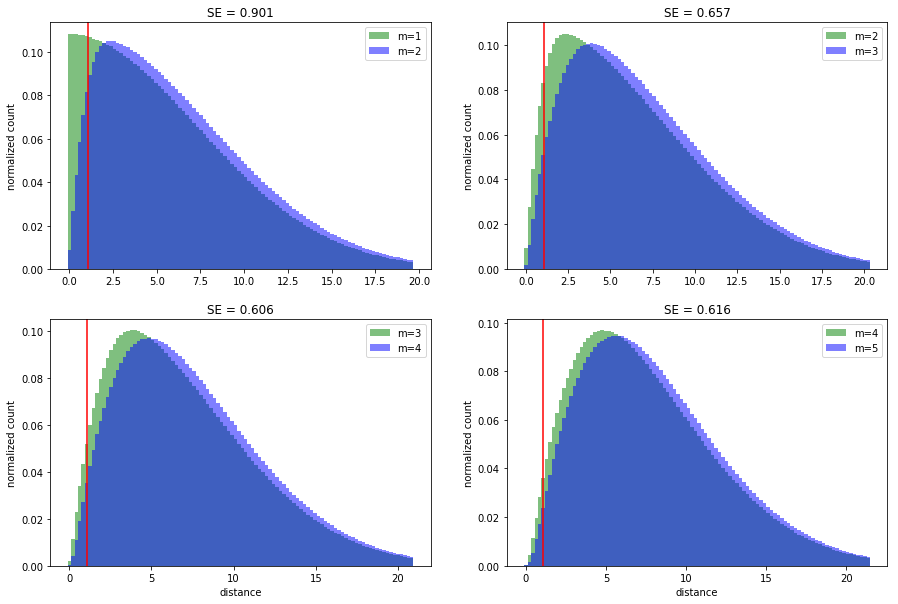
\includegraphics[width=\textwidth]{./Images/se_anal.png} }
  \caption[Histograms of distances in embedding space.]{Histograms of pairwise distances between vectors in embedding space for gradually increasing embedding dimension $m$. The vertical red line indicates the value of the tolerance parameter $r=0.2*\mathrm{std}(x)$. We can see histograms shifting to the right with increasing embedding dimension and progressively overlapping more. This means that for high embedding dimensions, sample entropy will be small for any value of tolerance parameter $r$.}
\label{fig:se-anal}
\end{figure}
The algorithm for computing sample entropy, described in Section~\ref{sec:se-theory}, requires selection of the embedding dimension $m$ and the tolerance parameter $r$. Embedding dimension $m$ is usually set to 1 or 2 and tolerance parameter $r$ is usually set at $0.1*\mathrm{std}(x)$ to $0.25*\mathrm{std}(x)$~\cite{jie2014emotion}. As can be seen in Table~\ref{tab:se-exp}, in all of the studies we evaluated, in spite of various applications and time series lengths, the same values were selected for $m$ and $\tau$, in particular, $m=2$ and $r=0.2*\mathrm{std}(x)$, where $\mathrm{std}(x)$ denotes standard deviation of the original time series. In Figure~\ref{fig:se-anal}, we can see why this is a reasonable choice. It shows histograms of pairwise distances in the embedding space for two successive embedding dimensions. With increasing embedding dimension, the histograms gradually overlap more, and for very high embedding dimensions, sample entropy becomes small for any $r$. Moreover, the histograms shift to the right, which requires higher value of $r$, but $r$ is a measure of the degree to which vectors are judged ``similar'', and thus should be kept low - for $r \geq \max_{i\in\{1,2,\dots,N\}} x_i$, all vectors will be counted in both embedding spaces and sample entropy is (approximately) zero.\footnote{The lowest value sample entropy can reach is $-\ln(2/\left( (N-m-1)(N-m)\right))$~\cite{richman2000physiological}.} For these reasons, we decided to follow the general concensus, and selected $m=2$ and $r=0.2*\mathrm{std}(x)$~\cite{hauge2011nonlinear, acharya2015novel, jie2014emotion, song2012automatic, acharya2012automated, mahajan2015unsupervised}.

\begin{table}[tbp]
  \centering
\begin{tabular}{|c|c|c|c|c|c|}
\hline
$\mathbf{r}$ & $\mathbf{m}$ & \textbf{Sampling Frequency} & \textbf{Recording Time} & \textbf{Application} & \textbf{Reference} \\ \hline
$0.2 * \mathrm{std}(x)$ & 2 & - & 256 min & depression &~\cite{hauge2011nonlinear} \\ \hline
$0.2 * \mathrm{std}(x)$ & 2 & 256 Hz & 5 min  & depression &~\cite{acharya2015novel} \\ \hline
$0.2 * \mathrm{std}(x)$ & 2 & 512 Hz & 63 s & emotion recognition &~\cite{jie2014emotion} \\ \hline
$0.2 * \mathrm{std}(x)$ & 2 & 173.6 Hz & 23.6 s & epilepsy &~\cite{song2012automatic} \\ \hline
$0.2 * \mathrm{std}(x)$ & 2 & 173.6 Hz & 23.6 s & epilepsy &~\cite{acharya2012automated} \\ \hline
$0.2 * \mathrm{std}(x)$ & 2 & 128 Hz & 30 s & denoising &~\cite{mahajan2015unsupervised} \\ \hhline{=|=|=|=|=|=}
$0.2 * \mathrm{std}(x)$ & 2 & 250 Hz & 60 s & depression & - \\ \hline
\end{tabular}
\caption[Literature review of SE $r$ and $m$ parameters.]{Summary of choices for the embedding dimension $m$ and tolerance $r$ parameters for sample entropy applied to EEG signals we found across literature. Note that all choices for $m$ and $r$ are the same.}
\label{tab:se-exp}
\end{table}
\subsection{Frequency Band Amplitudes} \label{sec:band-ampl}
Although our focus in this study is to examine the relationship between depression scores, treatment response and nonlinear measures, we also computed the mean frequency amplitudes in alpha, beta, gamma, delta and theta frequency bands using discrete fast Fourier transform by averaging the amplitudes corresponding to the frequencies in the respective bands. Figure \ref{fig:mba} shows an example result for FP1 amplitude of a randomly selected patient. Then, we performed the analysis of differences between various subgroups described in Section \ref{sec:distanal}. No significant differences between any two of the studied subgroups were found, and the mean amplitude values exhibited large variance between individual patients. Therefore, we decided to not pursue this approach of frequency band analysis further in this study.

\begin{figure} 
\centering
\noindent\makebox[\textwidth]{%
  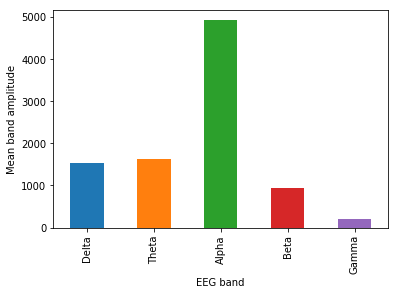
\includegraphics[width=0.7\textwidth]{./Images/mba.png} }
  \caption[An example range of mean band amplitudes.]{An example distribution of mean band amplitudes in channel FP1 of a randomly selected recording.}
\label{fig:mba}
\end{figure}

\subsection{Summary of Parameters}
In this section, we described our process for selecting the parameters used for computation of the nonlinear measures. In the rest of this chapter, all presented results were obtained using the values of nonlinear measures computed in manner described above. For the purpose of clarity, in Table~\ref{tab:paramsum}, we include the summary of the selected parameters.
\begin{table}[tbp]
\centering
\begin{tabular}[t]{|c|c|c|}
\hline
\textbf{Measure} & \textbf{Parameter} & \textbf{Value} \\ \hline
LLE              & $m$                & 10             \\ \cline{2-3}
                 & $\tau$             & 3              \\ \cline{2-3}
                 & $w_t$              & 50             \\ \cline{2-3}
                 & $t_e$              & 30             \\ \hline
CD               & $m$                & 15             \\ \cline{2-3}
                 & $\tau$             & 4              \\ \cline{2-3}
                 & $w_t$              & 50             \\ \cline{2-3}
                 & metric             & Chebyshev      \\ \cline{2-3}
                 & $r$                & GP on $(0.05,10)$ \\ \hline
\end{tabular}
\begin{tabular}[t]{|c|c|c|}
\hline
\textbf{Measure} & \textbf{Parameter} & \textbf{Value} \\ \hline
DFA              & $n$                & GP on $(4,320)$   \\ \cline{2-3}
                 & offset             & 50             \\ \cline{2-3}
                 & segment overlap    & 50\%           \\ \hline
HE               & $n$                & GP on $(0,20)$   \\ \hline
HD               & $k_{\mathrm{max}}$ & 50   \\ \hline
SE               & $m$                & 2   \\ \cline{2-3}
                 & $r$                & $0.2*\mathrm{std}(x)$   \\ \hline
\end{tabular}
\caption[Summary of parameters.]{Summary of parameters used for computation of the nonlinear measures. The abbrevation GP refers to geometric progression.}
\label{tab:paramsum}
\end{table}

\subsection{Surrogate Analysis} \label{sec:surrogate-analysis}
As mentioned in Section~\ref{sec:surrogate-analysis-theory}, surrogate analysis for high condifence levels requires generating surrogate dataset tens of times larger than the original dataset, and computing corresponding nonlinear measures for these surrogate signals. For instance, to achieve confidence level $\alpha = 95 \%$ for our dataset, this translates to generating $266*19*38 = 192052$ surrogate samples and computing on them each nonlinear measure considered in our study. Since nonlinear algorithms considered (described in the preceding subsections) are relatively computationally expensive, performing surrogate analysis for all measures and all patients is computationally infeasible. Thus, we analyzed each algorithm (with varying parameters) on a single recording (patient number 75, second session), using 19 surrogate samples. For generating the surrogate data, we used the iAAFT algorithm described in Section~\ref{sec:iaaft}. Note that to perform this as a test of nonlinearity, we have to assume that the choice of embedding parameters for the algorithms is correct.

An example of a result of such analysis for the largest Lyapunov exponent (embedding dimension 10, time delay 3) can be seen in Figure~\ref{fig:surr-lyap}; the results for other measures were similar. First, we can observe that the distribution of the values computed for the surrogate data does not seem normal for all channels. As mentioned in Section~\ref{sec:surrogate-analysis-theory}, this increases the required value sigma to achieve the same confidence, or requires performing a rank based test. It can be easily observed, then, that based on the rank based test, the hypothesis of a linear stochastic process cannot be rejected on (admittedly relatively low) confidence level $\alpha = 1 - 2/(19+1) = 90 \%$ for all channels except FP2, C4, T4, Pz. Obviously, does not necessarily imply that the process underlying corresponding time series is stochastic, because, for example, there still may be other nonlinear measures (or different choice of embedding parameters) which can discriminate between the original time series and the surrogate data. Neither does it suggest that the choice of embedding parameters is incorrect, because the process underlying corresponding time series may be stochastic. It is simply a failed attempt at disproving the null hypothesis of a stochastic linear process. Moreover, all our analyses concerned only a single patient.

\begin{figure} 
\centering
\noindent\makebox[\textwidth]{%
  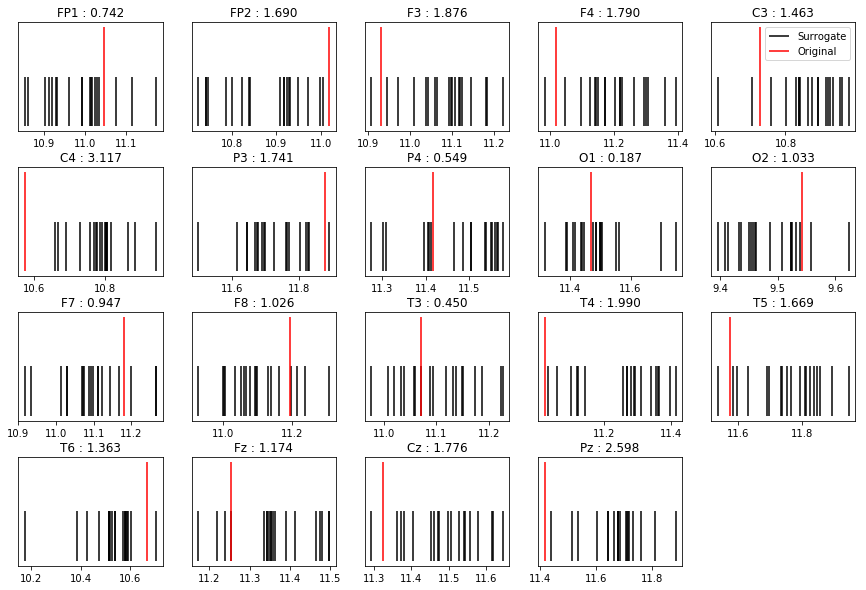
\includegraphics[width=1.0\textwidth]{./Images/surrogate/lyap_10_3_50.png} }
  \caption[Example distribution of $\lambda_1$.]{Example distribution of the largest Lyapunov exponent (embedding dimension 10, time delay 3) for 19 surrogate samples and the original for all channels. The number next to each channel name represents the confidence in sigma, computed as in equation~\ref{eq:sigma}.}
\label{fig:surr-lyap}
\end{figure}
\subsection{Nonstationarity}
To reduce the effects of possible nonstationarity, we attempted to find the most stationary window of the desired length using the stationarity test described in Section~\ref{sec:stationarity}. However, we found that selecting the least stationary window using this test did not improve the results as measured by the surrogate data analysis in Section~\ref{sec:surrogate-analysis}. This may be beacause the optimal effectiveness of AAFT and iAAFT the first and last point of the window should have the same value~\cite{andreas2000}. Moreover, selecting a different time window for each channel may result in inaccurate representation of the mental state by the vector of measures computed across channels. Therefore, it may be beneficial to use the same time window for all channels. If the results are dependent on the time during recording, then it would be advisable to select a fixed time window for all samples. Thus, we decided to skip this window selection step and pick a fixed time window for all channels and all recordings.
\section{Analysis of Measure Distributions between Groups} \label{sec:distanal}
\subsection{Before and After Treatment Groups} \label{sec:analbefaft}
As the first step of our analysis, we conducted an investigation of the differences in the nonlinear measures computed from the signals obtained before and after treatment. The purpose of this inquiry is to determine brain regions and measures affected by treatment. This is warranted by the fact that the patterns in EEG signals tend to be relatively stable over time. \add{This should be cited!} On the other hand, we realize the limitations of this attempt in the case of this study, since each patient recieved personalized method of treatment, and the methods may have differing impact.

For each group, we performed two-sided Kruskal-Wallis test for the null hypothesis that the distributions of values computed for measurements before and after treatment are the same. No significant differences in distributions were found for DFA, HE, and HD, $D_2$ and $\lambda_1$ computed using automatic selection of embedding parameters. Therefore, we include only results for the remaining measures. The results can be seen in Table~\ref{tab:bameans} in the Appendix.\footnote{In all tables, the p-value cutoffs for significance ratings are 0.05, 0.01, 0.005.} No significant differences between the groups are observed in DFA and HE values, and HD and CD show differences only in left temporal areas (T3, T4). On the other hand, LLE shows signficant differences in frontal (F3, F4), ``central'' (C3, C4) and left temporal (T3) areas, with similar, yet less signficant differences in those areas are observed for SE values.

Differences in the mean values of each measure in each electrode before and after treatment are visualized in Figure~\ref{fig:befaft}. Length of the error bars corresponds to two standard deviations. One can notice, for example, that values of LLE tend to be higher before treatment. As we will comment more in Section~\ref{sec:analrespdif}, this effect seems especially pronounced in the group responding positively to the treatment. 

Finally, we analyzed the differences in the before and after treatment recordings in the groups specifically responding and nonresponding to the treatment in Section~\ref{sec:analdepdif}. Moreover, we performed unsupervised analysis of before and after groups using PCA in 2,3, and 4 dimensions, and compared centroids and mean distances between before and after treatment recording for each group. However, the resulting plots and heatmaps are featureless and thus we will leave them out. The mean distances are also uninformative.

One notable outcome of these analyses is how relatively stable nonlinear measures are across time for individual patients. In Figure~\ref{fig:rel-change}, which shows relative differences between before and after treatment recordings for each patient and mean of each measure across channels, one can see that the relative changes for each measure remain comparatively small. The smallest relative change is observed for LLE and CD, whereas the largest are observed in DFA and SE. The intraindividual specificity of nonlinear measures, especially correlation dimension, has been noted in the literature, and has been suggested as a viable method of personal identification~\cite{schmid1996indications, poulos2002person, dunki2000intraindividual}.

\subsection{Low and High Depression Score Groups} \label{sec:analdepdif}
As mentioned in Section~\ref{sec:dataset}, studied dataset lacks symptom absent group, which makes the task of creating a generally applicable classifier for depression diagnosis more difficult. The patients, however, still vary in severity of their symptoms, which allows us to study correlation between symptom severity (which may, in turn, inform the task of finding a classifier). To this goal, we explored the differences in distributions of computed nonlinear between groups of the ``healthiest'' and most depressed patients visually and using statistical tests, and in this section, we present some of the results.

With the goal of analyzing the differences between the lightest and most severe symptoms, we selected two classes of recordings for analysis in this section as follows. The first class, called \emph{healthy}, of 50 recordings with reported depression score $\leq$ 16, and the second class, called \emph{depressed}, of 50 recordings with depression score $\geq$ 28. We should recognize that including after treatment recordings does not control for possible effects of treatment not reflecting in the depression scores but reflecting in the signal, or the inverse. Indeed, all the healthy recordings were made after treatment, and most of the depressed recordings were made before treatment.

First, we inspected histograms of computed measures between the two groups. There were striking trends in the means of the two distributions in almost all channels for all measures except correlation dimension. Means of depressed recordings are typically shifted to the left of the mean of healthy recordings for all measures except for largest Lyapunov exponent, for which the means are shifted to the right. For correlation dimension, the distributions in both groups are similar. Figure~\ref{fig:lyapdepdist} in the Appendix, which shows the distributions of the largest Lyapunov exponents for both groups, exemplifies the differences.  

Next, we investigated at the correlations between the individual measures and correlation scores. Figure~\ref{fig:dfadepcorr} shows visually clear negative correlation for DFA, and Figure~\ref{fig:lyapdepcorr} shows positive correlation for the largest Lyapunov exponent. Correlation dimension shows no significant correlations between depression scores on any channel, whereas the remaining measures are significantly correlated in almost all channels, and all those correlations are negative. Trends similar to the one observed for DFA were observed for Hurst exponent and Higuchi's fractal dimension, where, however, DFA shows slightly more significant correlations. Sample entropy values were significantly negatively correlated only on F4 and T6 channels. We also visualized correlations of individual measures to the the depression score and treatment response label on topographic scalp in Figure~\ref{fig:scalp-corrs}, and the corresponding p-values in Figure~\ref{fig:scalp-corrs-pval}. Interestingly, the patterns in p-values for depression score correlations seem almost centrally symmetrical for DFA, HE, and CD, and centrally symmetrical for LLE and SE.

Finally, we compared the distributions using Kruskal-Wallis test. Table~\ref{tab:depmeans} in the Appendix show the results. The mean values across all channels are significantly different for DFA, LLE, SE, and HD. The differences in DFA seem to be the most significant over parietal and occipital regions, and right parietal region (P4) in particular. Although LLE also exhibits differences in those areas, in addition, it shows slight differences in frontal (F4) area, and it is the right temporal region (T6) which shows the most pronounced differences. Similar behavior of significant differences across frontal, occipital, parietal, and right temporal region may be observed in SE and HD.

In contrast to previously observed lower EEG complexity (higher predictability) in depression~\cite{nandrino1994}, we find find that depressed patients exhibit slightly higher higher LLE and CD, indicating higher chaoticity and complexity, which implies lower predictibility. However, we used different method from the mentioned study to reach these conclusions.

\begin{figure} 
\centering
\noindent\makebox[\textwidth]{%
  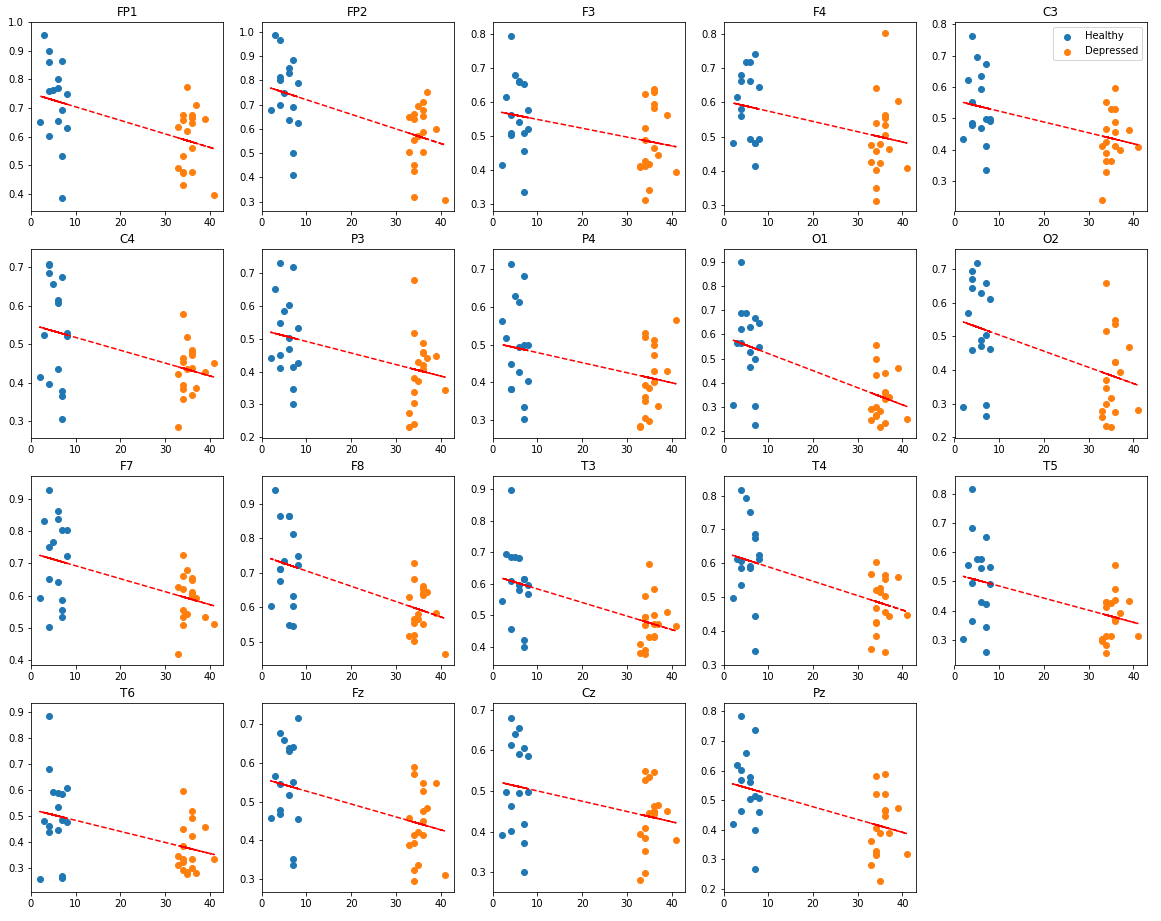
\includegraphics[width=1\textwidth]{./Images/dists/dfadepcorr.png} }
  \caption[Trends in DFA as a function of depression score.]{Trend of values of DFA as a function of depression score. The correlation is significantly ($p$ < 0.05) negative for all channels with exception of F3, F4, C3, P3, T3, Cz. Similar trend is present in Hurst exponent, Higuchi's fractal dimension and sample entropy. No correlation of correlation dimension with depression score is significant in any channel.}
 \label{fig:dfadepcorr}
\end{figure}

\begin{figure} 
\centering
\noindent\makebox[\textwidth]{%
  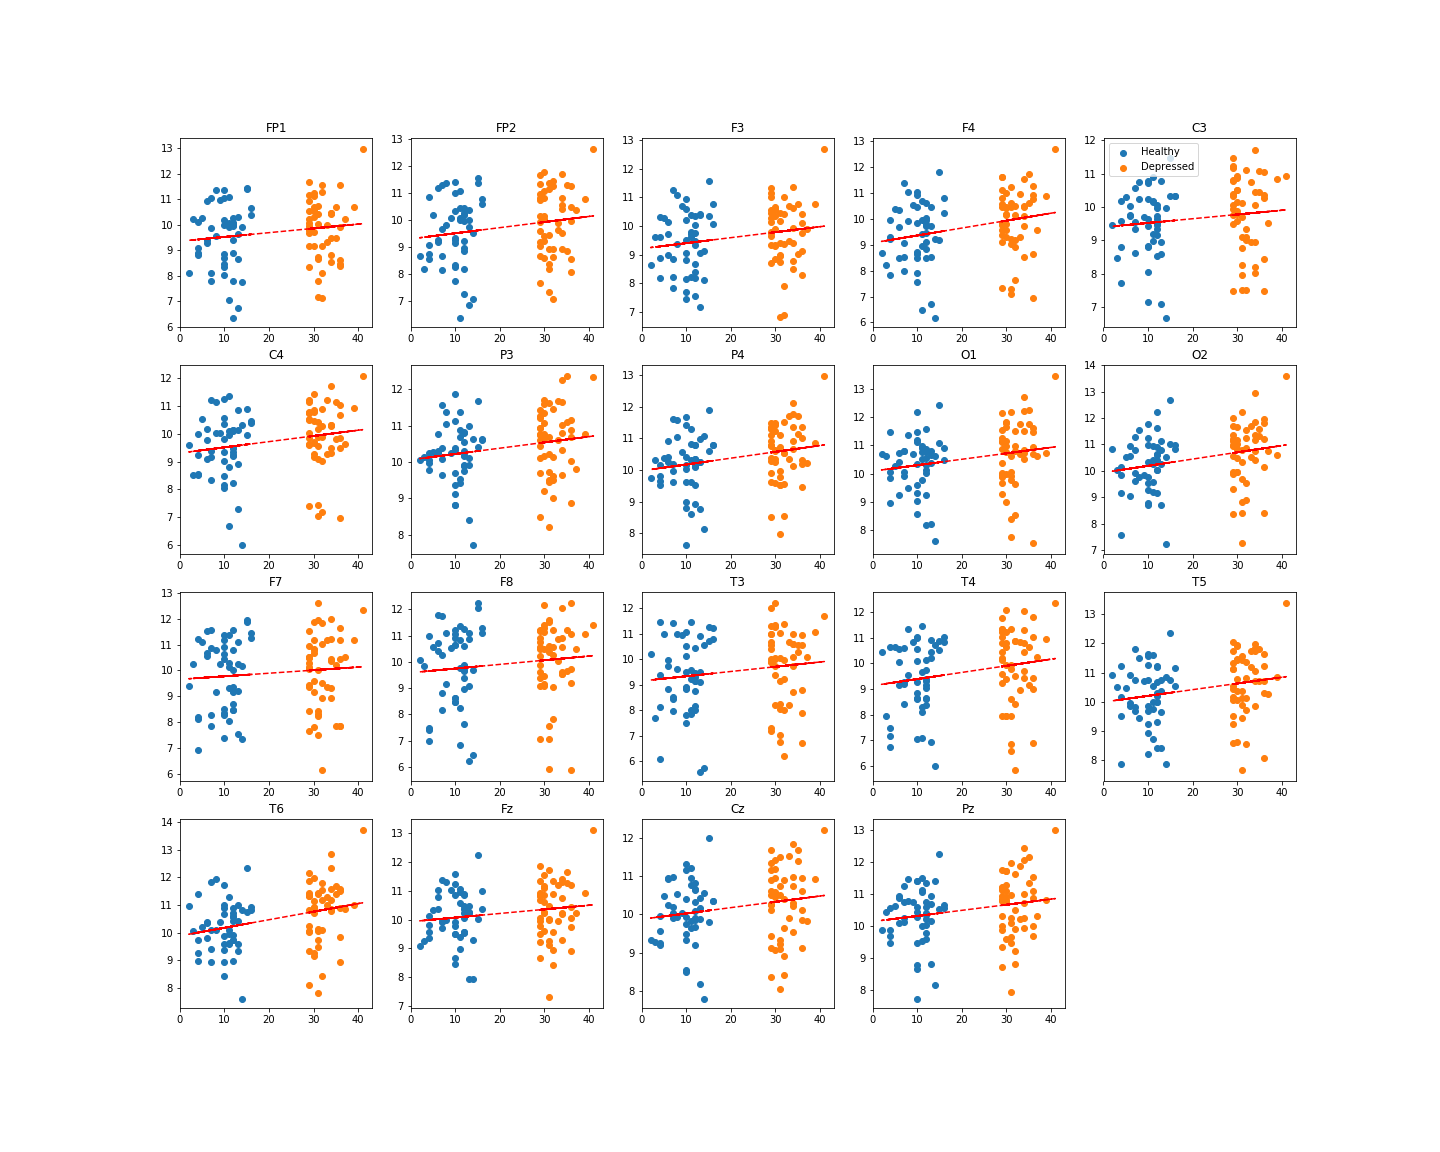
\includegraphics[width=1\textwidth]{./Images/dists/lyapdepcorr.png} }
  \caption[Trends in $\lambda_1$ as function of depression score.]{Trends of values of largest Lyapunov exponent as a function of depression score. The correlation is significantly ($p$ < 0.05) positive for all channels with exception of FP1, FP2, C3, F7, F8, T3.}
 \label{fig:lyapdepcorr}
\end{figure}

\begin{figure}
  \centering
  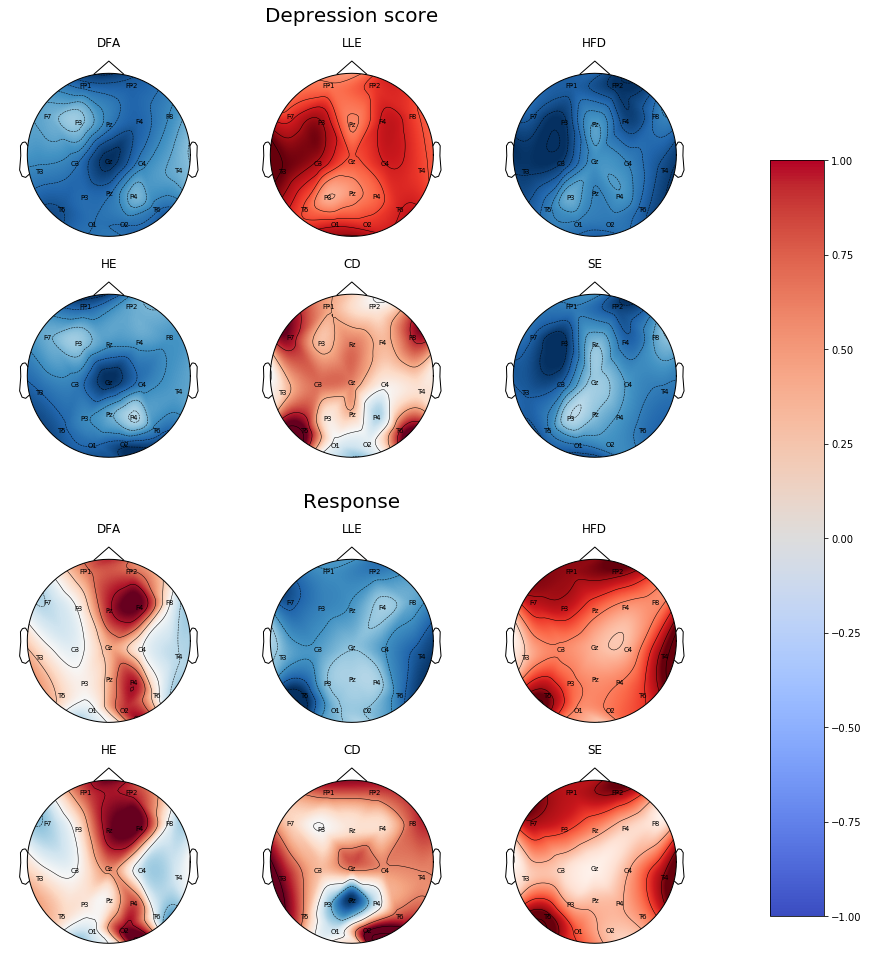
\includegraphics[width=\linewidth]{./Images/scalp_corr_all.png}
  \caption[Topographic correlation map.]{Topographic map of correlation coefficients on a scalp for depression diagnosis and response prognosis respectively. Color at each channel marks the value of Pearson's correlation coefficient between the value of corresponding measure and either depression score or treatment response label. The colors are then interpolated for smooth transitions. For depression score, all patients were included, whereas for response, only before treatment recordings were included.}
  \label{fig:scalp-corrs}
\end{figure}

\begin{figure}
  \centering
  \includegraphics[width=\linewidth]{./Images/scalp_corr_sig.png}
  \caption[Topographic map of the correlation p-values.]{Topographic map of correlation coefficients' p-value on a scalp for depression diagnosis and response prognosis respectively. Color at each channel marks the value of Pearson's correlation coefficient's p-value between the value of corresponding measure and either depression score or treatment response label across all patients. The colors are then interpolated for smooth transitions. For depression score, all patients were included, whereas for response, only before treatment recordings were included.}
  \label{fig:scalp-corrs-pval}
\end{figure}

\subsection{Low and High Response Groups} \label{sec:analrespdif}
Neurocorrelates of remission, or, in other words, positive response to a treatment, are interesting apart from the neurocorrelates of depression itself. Instead of indicating whether a treatment should be prescribed in the first place, the effects of various drugs on the brain may help in designing more individualized treatments, or in developments of new drugs, even for other conditions. However, as noted in Section~\ref{sec:dataset}, in our dataset, different kinds of treatments (including rTMS) are mixed for most patients, thus make the task of distinguishing the singular causes of any observed changes challenging. Nevertheless, we may still attempt to find discrepancies between the responding and stagnant patients. If we assume that any prescribed treatment was beneficial, we may be able identify traits of patients who are difficult to treat. Indeed, medical literature recognizes entire categories of such patients~\cite{kane1996factors}.

For each patient, we computed a measure of change in depression scores (and, by extension, of effectivity of the treatment) we call \emph{response} (RES). If $\mathrm{DS}_0$ denotes the depression score measured on the first visit and $\mathrm{DS}_4$ denotes the depression score measured on the second visit after 4 weeks, then response is computed as their ratio $\mathrm{RES} = \mathrm{DS}_4 / \mathrm{DS}_0$. Mean response is 2.47, mode 1.66, standard deviation 3.14. Most values range from 1 to 5, with a few outliers improving their symptoms 14 and 16-fold respectively. Only 9 patients stagnated exactly or slightly worsened their symptoms (response $\leq$ 1). Subsequently, we sampled 50 patients with the lowest value of response we call \emph{nonresponding} (nonresponders) and 50 patients with the highest value of response we call \emph{responding} (responders). 

We performed Kruskal-Wallis test to see the differences in the computed measures between the two groups in individual channels, considering only the before treatment recordings. The most significant differences found were in Lyapunov exponent, especially in frontal, parietal, and right temporal areas. Aside from the largest Lyapunov exponent, Higuchi's fractal dimension then also showed significant differences in frontal areas.. The results are shown in Table~\ref{tab:remmeans} in the Appendix. In comparison with Section~\ref{sec:analdepdif}, these results suggest that, with exception of LLE, differences in nonlinear measures between responders and nonresponders in the recordings obtained before treatment are considerably less significant than differences in depression score. On the other hand, it is possible that the differences are less significant due to smaller dataset size, since the test is performed on smaller number of samples. For completeness, we also decided to include comparison which includes both before and after treatment recordings, which can be seen in Table~\ref{tab:remmeansext}.

Moreover, we also compared before and after treatment recordings of responding, and before and after treatment recordings of nonresponding patients. Significant differences were found only in LLE, CD and SE, for which the results can be seen in the Appendix in Tables~\ref{tab:llebaresp},~\ref{tab:d2baresp}, and~\ref{tab:sebaresp} respectively. These differences are also visualized in Figures~\ref{fig:respnon1},~\ref{fig:respnon1auto}, and~\ref{fig:respnon2} in the Appendix. We can see, for example, that the mean values of LLE across channels are higher before treatment for the responding group, but this effect is less pronounced for the nonresponding group, where depression score also slightly descreased. Since this group also received treatment, the observed higher depression score accompanied by LLE increase is not due to the effects of treatment. Together with Table~\ref{tab:remmeans}, this result further supports the hypothesis that it is the decrease in depression score which results in higher values of LLE.

Of course, analyzing effectivity of treatment is difficult problem, and we realize the many limitations of this analysis. For example, many variables, including age, sex, starting depression score, behavioral changes occuring in the interim period and the kind of treatment, were not accounted for. Moreover, many of the patients selected as nonresponding actually improved their symptoms slightly. In fact, symptoms of only 9 patients of the whole dataset worsened or stayed stagnant. No significant differences between before and after treatment recordings of these ``strictly'' nonresponding patients, were found. Thus, one possibility of strengthening the differences between the responding and nonresponding groups may be to include the after treatment recordings for the ``strictly'' nonresponding group to the nonresponding group. However, we decided against doing this, because some differences in the before and after treatment groups for the ``strictly'' nonresponding patients may have remained insignificant due to small size of this group.

\section{Results} \label{sec:results-nl}
\subsection{Methodology}
We used two classifiers: Logistic Regression (LR) and Support Vector Machine (SVM). One third of randomly selected samples was held out as a test set, the rest was used for training and cross validation. The following feature selection algorithms were evaluated with LR (regularization strength 1) and SVM (regularization strength 1 and linear kernel, i.e. $k(\vec{x_1}, \vec{x_2}) = \vec{x_1} \cdot \vec{x_2}$):
\begin{itemize}
  \item recursive feature elimination with 3-fold cross validation based on coefficients of the linear model,
  \item elimination of features with below-mean coefficients of the linear model,
  \item selection of 5 features with the highest $\chi^2$ statistics between values of the feature and corresponding class,\unsure{Am I justified in using $\chi^2$?}
  \item genetic algorithm with 5-fold cross validation (scoring models based on ROC AUC, population size 80, 80 generations, crossover probability 0.8, mutation probability 0.2, and tournament size 5),
  \item manual selection of channels with significantly different means of corresponding features between the two considered classes, as reported by the Kruskal-Wallis test.
\end{itemize}
Out of those feature selection techniques, genetic algorithm was by far the most effective. However, most of the best performing and thus reported classifiers were found by combination of the last two techniques, i.e. by applying genetic selection algorithm to the subset of channels marked as having differing means between the two groups.

Evaluation was performed using 5-fold cross-validation. The best performing classifiers (based on accuracy, precision, recall, f-score, and number of features) were selected for each measure and for all measures by varying the maximum number of features considered by the genetic algorithm from 3 to the 1/10 of the corresponding training set size. Then, a brute force grid search with 5-fold cross validation was performed on each classifier to select 
\begin{itemize}
  \item the optimal regularization stength, and norm for LR, and
  \item the optimal regularization strength and kernel type (linear, polynomial, or radial basis function with coefficients $\gamma = 1/n_f$, where $n_f$ is the number of selected features) for SVM. \unsure{Am I justified in changing the kernel type?}
\end{itemize}
This resulted in slight improvement in accuracy, and correspondingly slight bias of the reported classifiers.

\subsection{Depression Diagnosis}
\begin{figure}
\centering
\begin{subfigure}{0.45\textwidth}
  \centering
  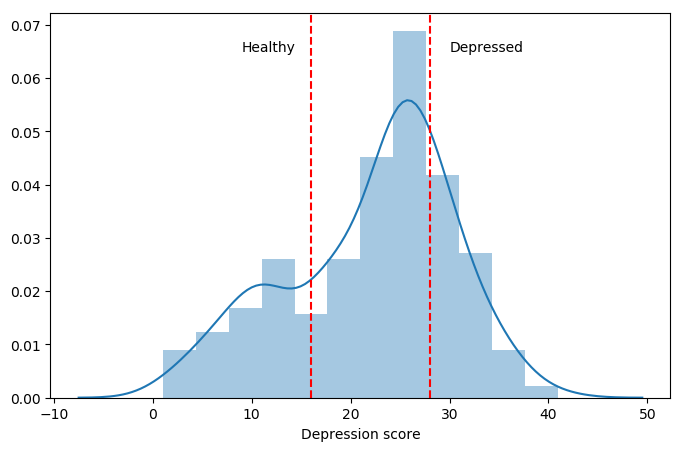
\includegraphics[width=\linewidth]{./Images/labels_dep.png}
  \caption{Label thresholds for depression diagnosis.}
  \label{fig:labels-dep}
\end{subfigure}%
\begin{subfigure}{0.45\textwidth}
  \centering
  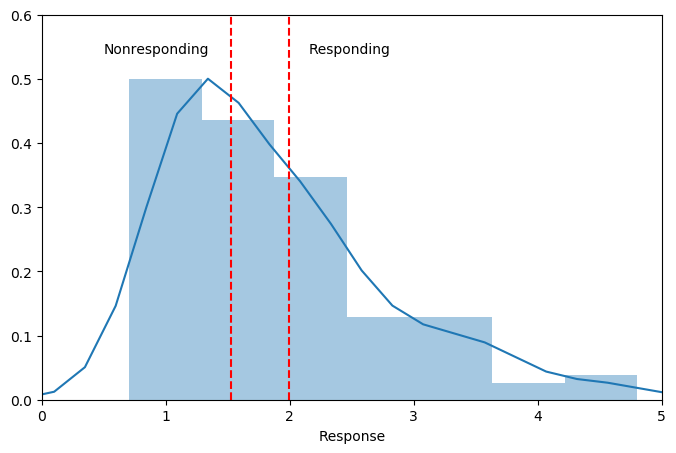
\includegraphics[width=\linewidth]{./Images/labels_rem.png}
  \caption{Label thresholds for response prognosis.}
  \label{fig:labels-rem}
\end{subfigure}
\caption[Label selection for corresponding tasks.]{Label selection for diagnosis and prognosis tasks. The thresholds were selected such that enough samples was present in each class, and such that the classes remained balanced.}
\label{fig:labels}
\end{figure}
The recordings were separated into two classes as follows:
\begin{description}
  \item[Healthy]: 50 recordings with associated depression score at most 16.
  \item[Depressed]: 50 recordings with associated depression score at least 28.
\end{description}
These thresholds are visualized on the distribution of depression scores in the dataset in Figure~\ref{fig:labels-dep}. The results are shown in Table~\ref{tab:depcl}. The best performing classifiers in this section were SVMs. The largest Lyapunov exponent was the most predictive out of all considered nonlinear measures, both achieving the highest accuracy out of the single-measure classifiers ($0.72 \pm 0.04$), and being one of the measures in majority of the best performing combined-measure classifiers. It was followed, perhaps surprisingly considering the results obtained in Section~\ref{sec:analdepdif}, by correlation dimension ($0.71 \pm 0.05$). Although the accuracy of the remaining classifiers, whose features were obtained using the Kruskal-Wallis test from Section~\ref{sec:analdepdif}, was slightly lower (with higher variance), they are also simpler in terms of the number of selected channels.

All the channels in the combined-measure classifiers were found using the genetic algorithm, as described in the opening to this section. The best overall accuracy was achieved by combination of the largest Lyapunov exponent and sample entropy ($0.75 \pm 0.10$). However, second to it was a combination of the largest Lyapunov exponent and correlation dimension, which has lower variance ($0.74 \pm 0.04)$. Other measures performing well together with the largest Lyapunov exponent are the Hurst exponent, and sample entropy together with DFA. The best combination not inluding the largest Lyapunov exponent is correlation dimension and Higuchi's fractal dimension.

In Section~\ref{sec:analdepdif}, we have seen that correlations of LLE with depression score are the most significant of all measures, which may explain why in this section, we found LLE to be the most discriminative measure. Moreover, we have seen that the differences between depressed and healthy patients are the most significant in the temporal areas for all measures, which may explain the relatively high rate of selection of the T3 and T6 channels.

Consistency in the selected channels for a fixed measure might indicate a relationship between activity captured by the nonlinear measure in the brain region local to the channel and corresponding label. However, the selected features seem inconsistent across classifiers using mixed measures or a single measure included in the mix. One possible explanation is that different measures complement themselves in such a way that different channels are relevant when classification is performed based on single measure as opposed to a combination of measures.

Although the obtained accuracies are notably lower than those obtained in studies we reviewed in Section~\ref{sec:applications}, these results are not directly mutually comparable. Most importantly, all the reviewed studies employed a control group of symptomless, healthy patients, whereas our dataset composed entirely of patients suffering from depression with various degree of symptom severity. Nevertheless, the obtained accuracies are substantial, suggesting possible nonsaturating relationship between depression severity and nonlinear measures recorded in EEG signals obtained from various cortical regions.

\begin{table}[tbp]
\centering
\scriptsize
\begin{tabular}{|c|c|c|c|c|c|c|c|c|c|c|}
\hline
\textbf{Measure} & \textbf{Classifier} & \multicolumn{2}{c}{\textbf{Accuracy}} \vline & \multicolumn{2}{c}{\textbf{Precision}} \vline & \multicolumn{2}{c}{\textbf{Recall}} \vline & \multicolumn{2}{c}{\textbf{F-score}} \vline & \textbf{Channels} \\ \hline
& & \textbf{Mean} & \textbf{Std} & \textbf{Mean} & \textbf{Std} & \textbf{Mean} & \textbf{Std} & \textbf{Mean} & \textbf{Std} & \\ \hline
LLE, SE & SVM (lin.) & \textbf{0.75} & 0.10 & 0.77 & 0.09 & 0.75 & 0.10 & 0.75 & 0.10 & \makecell{\emph{LLE}: C4, T3, T6, Pz \\
                                                                                                         \emph{SE}: C3, P4} \\ \hline 
LLE, CD & SVM (lin.) & 0.74 & 0.04 & 0.76 & 0.04 & 0.74 & 0.04 & 0.74 & 0.05 & \makecell{\emph{LLE}: F3, F7, T6 \\
                                                                                                         \emph{CD}: O1, O2, T5 } \\ \hline 
LLE, HE & SVM (lin.) & 0.73 & 0.06 & 0.74 & 0.06 & 0.73 & 0.06 & 0.73 & 0.06 & \makecell{\emph{LLE}: P3, T3, T6, Pz \\
                                                                                                         \emph{HE}: C3, T3} \\ \hline 
LLE, SE, DFA & SVM (lin.) & 0.73 & 0.09 & 0.74 & 0.10 & 0.73 & 0.09 & 0.73 & 0.09 & \makecell{\emph{LLE}: T6, Fz \\
                                                                                                         \emph{SE}: T6 \\ 
                                                                                                         \emph{DFA}: P4} \\ \hline 
CD, HD & LR & 0.73 & 0.10 & 0.74 & 0.11 & 0.73 & 0.10 & 0.73 & 0.10 & \makecell{\emph{CD}: F3, Fz \\
                                                                                                \emph{HD}: P3, Cz} \\ \hhline{=|=|=|=|=|=|=|=|=|=|=}
LLE & SVM (lin.) & 0.72 & 0.04 & 0.73 & 0.04 & 0.72 & 0.04 & 0.72 & 0.04 & T3, T5, T6, Pz \\ \hline
CD & SVM (lin.) & 0.71 & 0.05 & 0.72 & 0.05 & 0.71 & 0.05 & 0.71 & 0.05 & F3, C4, P3, F8, T5, T6, Fz, Cz \\ \hline 
SE & LR & 0.68 & 0.12 & 0.69 & 0.12 & 0.68 & 0.12 & 0.68 & 0.12 & C4, O2, T6 \\ \hline
HD & SVM (rbf) & 0.67 & 0.11 & 0.67 & 0.12 & 0.67 & 0.11 & 0.67 & 0.11 & C3, C4, P4, T6, Cz \\ \hline
DFA & LR & 0.67 & 0.16 & 0.68 & 0.17 & 0.67 & 0.16 & 0.67 & 0.16 & F8, O2 \\ \hline
HE & LR & 0.67 & 0.17 & 0.68 & 0.18 & 0.67 & 0.17 & 0.67 & 0.17 & O2, T4 \\ \hline
\end{tabular}
\caption[Evaluation of depression diagnosis.]{Evaluation of depression classification. The two classes consist of 50 / 50 recordings with the smallest / highest associated depression score out of recordings performed both before and after administration of drugs.}
\label{tab:depcl}

\bigskip

\begin{tabular}{|c|c|c|c|c|c|c|c|c|c|c|}
\hline
% \textbf{Measure} & \textbf{Classifier} & \textbf{Accuracy} & \textbf{Precision} & \textbf{Recall} & \textbf{F-score} & \textbf{Channels} \\ \hline
\textbf{Measure} & \textbf{Classifier} & \multicolumn{2}{c}{\textbf{Accuracy}} \vline & \multicolumn{2}{c}{\textbf{Precision}} \vline & \multicolumn{2}{c}{\textbf{Recall}} \vline & \multicolumn{2}{c}{\textbf{F-score}} \vline & \textbf{Channels} \\ \hline
& & \textbf{Mean} & \textbf{Std} & \textbf{Mean} & \textbf{Std} & \textbf{Mean} & \textbf{Std} & \textbf{Mean} & \textbf{Std} & \\ \hline
LLE, SE & SVM (lin.) & \textbf{0.75} & 0.10 & 0.77 & 0.09 & 0.75 & 0.10 & 0.75 & 0.10 & \makecell{\emph{LLE}: FP2, F3, O1, T4, T6 \\
                                                                                                         \emph{SE}: F3, C3, T6 }  \\ \hline
LLE, CD& SVM (lin.) & \textbf{0.75} & 0.11 & 0.76 & 0.11 & 0.75 & 0.11 & 0.75 & 0.11 & \makecell{\emph{LLE}: F3, O2, T5, T6 \\
                                                                                                        \emph{CD}: FP2, F4, O2 } \\ \hhline{=|=|=|=|=|=|=|=|=|=|=}
LLE & LR & 0.71  & 0.08  & 0.73  & 0.08  & 0.71  & 0.08  & 0.70  & 0.09  & F3, F4, T5, T6 \\ \hline 
CD & LR & 0.67 & 0.09 & 0.70 & 0.11 & 0.67 & 0.09 & 0.65 & 0.10 & F3, F4, O2, Pz \\ \hline
HD & LR & 0.66 & 0.05 & 0.72 & 0.08 & 0.66 & 0.05 & 0.64 & 0.05 & F3, F8 \\ \hline
SE & LR & 0.66 & 0.09 & 0.66 & 0.09 & 0.66 & 0.09 & 0.65 & 0.10 & FP1, F3, P3, Cz \\ \hline
DFA & SVM (lin.) & 0.64 & 0.15 & 0.65 & 0.15 & 0.64 & 0.15 & 0.63 & 0.15 & T3, T4, Cz \\ \hline
HE & SVM (rbf) & 0.63 & 0.09 & 0.64 & 0.10 & 0.63 & 0.09 & 0.62 & 0.09 & C3, T6 \\ \hline
\end{tabular}
\caption[Evaluation of response prognosis.]{Evaluation of response classification. Only recordings obtained before drug administration were considered. The two classes consist of the 50 patients with the highest and least improvement in depression score after the drug administration (as measured by ratio of the two depression scores).}
\label{tab:respcl}
\end{table}
\subsection{Response Prognosis} \label{sec:nl-res-prog}
As we mentioned in Section~\ref{sec:analrespdif}, response is defined as the ratio of the depression score reported on the second session (after administration of drugs) to the depression score reported on the first session (before administration of drugs). For the task of predicting response to treatment, recordings were separated into two classes as follows:
\begin{description}
  \item[Nonresponding]: 50 recordings made before administration of drugs with the lowest response.
  \item[Responding]: 50 recordings made before administration of drugs with the highest response.
\end{description}

The results can be seen in Table~\ref{tab:respcl}. Again, the largest Lyapunov exponent was the most predictive nonlinear measure. Unlike for the depression diagnosis, sample entropy and correlation dimension were the only other nonlinear measures which were able to achieve accuracy above $70 \%$ both in combination with other measures and as stand-alone features. Interestingly, F3 channel seems to be considerably more relevant for response prognosis than for depression diagnosis.

In Section~\ref{sec:analrespdif}, we have observed the most significant differences between responders and nonresponders in the recordings obtained before treatment for LLE (especially F4 and T6 channels), which may explain that LLE is the most discriminative nonlinear measure for treatment response prediction. Although the differences for other measures remained relatively insignificant, CD, HD, and SE achieve accuracy of approximately 67\%. This may be explained by the fact that in Section~\ref{sec:analrespdif}, we tested only for the differences in distributions in values recorded on individual channels, whereas in this section, we perform classification based on combination of multiple channels.

By comparing our results to results of studies reviewed in Section~\ref{sec:applications-prog}, we can see that our results, obtained using nonlinear dynamical analysis and LLE in particular, is relatively competetive with some results in published literature focusing on relative frontal $\theta$ powers. Our results may therefore encourage effort in examination of nonlinear measures and LLE in relation to treatment response.

\subsection{Limitations}
\section{Implementation} \label{sec:impl-nl}
All the code used for this section is publicly available \href{https://github.com/mirgee/thesis\_project}{online}, as well as on the CD accompanying this text. Used programming language was Python. The plots were produced using \href{https://matplotlib.org/}{Matplotlib} library. Other used libraries include \href{http://www.numpy.org/}{NumPy} for vectorized computations, \href{https://scipy.org/scipylib/index.html}{SciPy} for signal processing algorithms, \href{http://pandas.pydata.org/}{Pandas} for data storage and manipulation, and \href{https://jupyter.org/}{Jupyter} for development.
 
For computation of nonlinear measures, we used slightly modified versions of \href{https://github.com/CSchoel/nolds}{nolds} library by C. Schölzel and published under MIT Licence, and \href{https://github.com/manu-mannattil/nolitsa}{nolitsa} library by M. Mannatil and published under 3-clause BSD licence. 

Hereby we provide a summary of used software:
\begin{description}
  \item[Public availability:] \href{https://github.com/mirgee/thesis\_project}{online}, accompanying CD
  \item[Main programming language:] Python
  \item[Plotting library:] \href{https://matplotlib.org/}{Matplotlib}
  \item[Vectorized computations:] \href{http://www.numpy.org/}{NumPy}
  \item[Signal processing algorithms:] \href{https://scipy.org/scipylib/index.html}{SciPy} 
  \item[Data storage and manipulation:] \href{http://pandas.pydata.org/}{Pandas} 
  \item[Execution environment:] \href{https://jupyter.org/}{Jupyter} 
  \item[Nonlinear Dynamical Analysis:] modifications of \href{https://github.com/CSchoel/nolds}{nolds} and \href{https://github.com/manu-mannattil/nolitsa}{nolitsa}
\end{description}

\chapter{Deep Learning Approach} \label{ch:dl}
\section{Convolutional Neural Networks}
In this section, we briefly introduce the Convolutional Neural Networks (CNNs), a class of neural network architectures, which we use in this chapter to perform the depression diagnosis and prognosis classification tasks.

\subsection{Mathematical Background}
In order to make some of the essential terms used in this chapter more concrete, we will provide their definitions in the following text. The first term requiring a definition is the term convolution, which gives the name to convolutional neural networks.
\begin{dfn}
  Let $I$ be an image function, $K$ a kernel. A (discrete) \textbf{convolution} of $I$ and $K$ is a linear operation defined as
  \begin{align}
    (I*K)(i,j) = \sum_m \sum_n I(m,n) K(i-m, j-n) \, .
  \end{align}
\end{dfn}

Note that some machine learning libraries (such as Tensorflow) implement \textbf{cross-correlation} instead of convolution, but preserve the term convolution for the operation \cite{tfnn2d}. Cross-correlation corresponds to convolution with kernel rotated by 180 degrees:
\begin{align}
  (I*K)(i,j) = \sum_m \sum_n I(m,n) K(i+m, j+n) \, .
\end{align}
Unlike convolution, cross-correlation is not commutative, but this property is not necessary for neural network applications \cite{goodfellow2016}.

When discussing the distinguishing properties of CNNs, we will use the the terms invariance and equivariance.
% \begin{dfn}
%   Let $f$ be arbitrary function, and $\mathcal{D}$ its degradation (or transformation) operator. We say $f$ is an \textbf{invariant} function under $\mathcal{D}$ if
%   \begin{align}
%     \mathcal{D}(f) \equiv f \, .
%   \end{align}
% \end{dfn}
% \begin{dfn}[\cite{pitts2013}]
%   Let $G$ be a group and $X$, $Y$ its G-sets. Then $F:X \rightarrow Y$ is called an \textbf{equivariant} function if
%   \begin{align}
%     F(g(x)) = g(F(x))
%   \end{align}
%   for all $G$ actions $g$ and $x \in X$.
% \end{dfn}

\begin{dfn}[\cite{pitts2013}]
  Let $f: X \rightarrow Y$ be arbitrary function, $G$ a group of transformations on $X$. We say $f$ is an \textbf{invariant} function under group of transformations $G$ if
  \begin{align*}
    f(T(x)) \equiv f(x), \qquad \forall T \in G, \, \forall x \in X.
  \end{align*}
  Moreover, if $G$ is a group and $X$, $Y$ its G-sets, then $f: X \rightarrow Y$ is an \textbf{equivariant} function under $G$ if
  \begin{align*}
    f(T(x)) \equiv T(f(x)), \qquad \forall T \in G, \, \forall x \in X.
  \end{align*}
\end{dfn}

Invariance to a transformation means that the if the transformation is applied to the input of the function, the output remains the same. Equivariance, on the other hand, means that if the transformation is applied to the input, the output is transformed in the same way. For example, as we will see in Section \ref{sec:pooling}, CNNs are invariant to local translation, but are not invariant to rotation, for example. Furthermore, convolution is an operation equivariant to translation \cite{goodfellow2016}.

A neural network can be viewed as a function approximation model based on an iterative optimization algorithm. There is a number of such algorithms in use, but many of them are variations of \textbf{gradient descent} algorithm, introduced by Werbos in 1974 \cite{werbos1974beyond}. Gradient descent is a first order iterative method of finding an extremum of a differentiable function $f : \RR^m \rightarrow \RR^n$, $f \in C^1$, based on continually moving a point in its domain space in the opposite direction of its gradient at that point, until the absolute value of the gradient is below a certain threshold. 

\begin{algorithm}
  \caption{A basic version of gradient descent algorithm. The parameter $\alpha$ is called the learning rate.}
  \label{alg:gd}
\begin{algorithmic}[1]
  \State Initialize random $x_0 \in \RR^n$,
  \State $n \gets 0$
  \State step\_size $\gets 1$  
  \While{step\_size $ < \text{threshold}$ and $n < $ iters\_limit}
  \State $x_{n+1} = x_n - \alpha * \mathrm{grad} f(x_n)$
  \State step\_size $\gets |x_{n+1} - x_n|$ 
  \State $n \gets n + 1$
  \State Optionally update $\alpha$
  \EndWhile
\end{algorithmic}
\end{algorithm}

The family of first order optimization methods is vast, including techniques such as stochastic variations of gradient descent \cite{robbins1951stochastic}, gradient descent with momentum \cite{rumelhart1988learning}, RMSProp (Root Mean Squared Propagation) \cite{tieleman2012lecture}, and Adam (Adaptive Moment estimation) \cite{kingma2014adam}. In Algorithm \ref{alg:gd}, we can see that gradient descent consists of two main steps: computation of the gradient $\mathrm{grad} f(x_n)$, and the parameter update. Most of the variations modify one at least one those steps, i.e. the step direction and its magnitude.

\subsection{History}
The classical approach to image pattern recognition consists, in general, of the following stages:
\begin{description}
  \item[preprocessing:] supressing unwanted distortions and noise, enhancement beneficient for further processing,
  \item[object segmetation:] separating disparate objects from the background,
  \item[feature extraction:] gathering relevant information about the properties of the objects, removing irrelevant variations,
  \item[classification:] categorizing segmented objects based on obtained features into classes.
\end{description}

The preprocessing step may require additional assumptions about the data or further processing, which are potentially too restrictive or too broad. Getting around this limitation requires dealing with complications such as high dimensionality of the input (number of pixels) and desirability of invariance to a number of allowable distortions and geometrical transformations.

Artificial neural networks in combination with gradient-based learning are one possible solution to the problem. By gradually optimizing a set of weights based on a training data set using a differentiable error function, they provide a framework for learning a suitable set of assumptions automatically from the data.

One of the oldest neural network architectures, fully connected multi-layer perceptron (FC-MLP), can be theoretically used for image pattern recognition. However, it has at least the following drawbacks \cite{lecun1999object}:
\begin{description}
  \item[parameter explosion:] the number of parameters of such network is exponential in the number of layers, increasing the capacity of the network and therefore need for more data,
  \item[no invariance:] no invariance even with respect to common geometrical transformation such as translation, rotation and scaling,
  \item[ignoring input topology:] natural images exhibit strong local structure and high correlation between intensities of neighboring pixels, but FC-MLPs are unstructured - inputs can be presented in any order.
\end{description}

Although the main idea of CNNs dates back to 1980, when K. Fukushima introduced neocognitron~\cite{fukushima1982}, the back-propagation algorithm was not widely known at the time. The first convolutional architecture successfully applied on an image pattern recognition problem by attempting to solve the aforementioned problems, dubbed LeNet-5, was proposed in 1998 by Y. LeCun, L. Bottou, Y. Bengio and P. Haffner~\cite{LeCun1998}.

\subsection{Properties} \label{sec:properties-cnn}
\begin{figure} 
\centering
\noindent\makebox[\textwidth]{%
  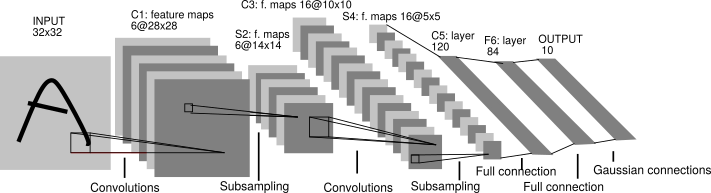
\includegraphics[width=0.8\textwidth]{./Images/lenet-5.png} }
  \caption[LeNet-5 architecture diagram.]{LeNet-5 architecture~\cite{lecun1999}.}
\label{fig:lenet-5}
\end{figure}

Being inspired by visual processing systems in biological organisms\footnote{As early as in 1968, D. H. Hubel and T.N. Wiesel discovered that some cells (called simple cells) in cat's primary visual cortex (V1) with small receptive fields (shared by neighboring neurons) are sensitive to straight lines and edges of light of particular orientation, and other cells (called complex cells) with larger receptive fields further in the visual cortex also respond to straight lines and edges, but with invariance to translation~\cite{Hubel1968}.}, LeNet-5 proposed the following design principles to enforce \emph{shift, scale and distortion invariance}~\cite{lecun1999}:
\begin{description}
  \item[local receptive fields:] each neuron in a layer receives input from a small neighborhood in the previous layer,
  \item[shared weights:] each layer is composed of neurons organized in planes within which each neuron have the same weight vector (feature map),
  \item[spatial subsampling:] adding a subsampling layers, which reduce the resolution of the previous layer by averaging or by taking the maximum value of neighboring pixels in the previous layer.
\end{description}
In the following, we will describe each of these properties and their implications in more detail.
\subsubsection{Local Receptive Fields} \label{sec:local-rec-fields}
\emph{Local receptive fields} enable the network to synthesize filters that produce strong response to elementary salient features in the early layers (such as lines, edges and corners in a visual input, and their equivalents in other modalities), and then learn to combine them in the subsequent layers to produce higher-order feature detectors. This property enables the models to induce the previously hardcoded filters from data.

\begin{figure} 
\centering
\noindent\makebox[\textwidth]{%
  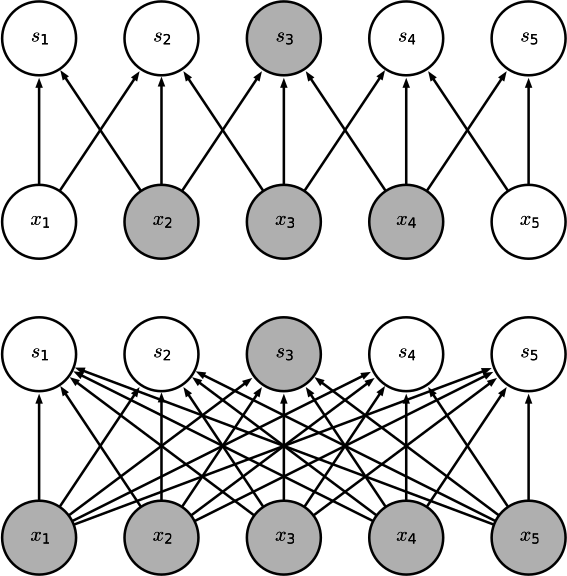
\includegraphics[width=0.5\textwidth]{./Images/receptive_field.png} }
  \caption[Receptive field.]{Receptive field~\cite{goodfellow2016}.}
\label{fig:receptive_field}
\end{figure}

For a visual explanation of the concept of receptive field, see Figure~\ref{fig:receptive_field}. The locality of of those receptive fields implies sparser connectivity, and hence more efficient computations in comparison with fully connected neural networks. A fully connected neural network with no hidden layers with $m$ inputs and $n$ outputs has $m \times n$ weight parameters, and the correspoding feed forward pass (matrix multiplication) is of $O(m \times n)$ time complexity per input. If the number of connections per output unit is limited to $k < m$, the achieved runtime is $O(k \times n)$, where $k$ is usally in practice several orders of magintude smaller than $m$~\cite{goodfellow2016}.

In shallow neural networks, locality of receptive fields implies locality of ``influence'' of each input unit on the output. In deep neural networks, on the other hand, units in the deeper layers can be indirectly connected to some or all units of the input, thus enabling them to achieve aforementioned effect of combining more complex features from simpler ones.

\subsubsection{Shared Weights} \label{sec:shared-weights}
With \emph{shared weights}, neural units in a layer with differing receptive fields have the same feature map and the same feature detecting operation (convolution with feature map kernel followed by additive bias and a application of a nonlinear function) is performed on differing parts of the image (see Figure~\ref{fig:shared_weights}). A single convolutional layer is composed of multiple feature detecting planes.

Shared weights principle exploits the fact that in natural images, a function of small number of neighboring pixels can be useful in multiple parts of the image. For example, an edge detector can be used accross the entire image to detect edges in the first layer, an object detector can then be used to detect presence of edges in particular arrangements in the next layer, etc.

Although it does not reduce the time complexity of the feedforward pass, it does reduce the memory requirements. If the kernel size is $k$, $m$ the number of inputs, $n$ the number of outputs, the number of parameters per layer is $k$ instead of $m \times n$ (per feature detecting plane) in a fully connected case. Since $k$ is usually in practice several orders of magnitude smaller than $m$, and usually $m$ and $n$ are comparable in size, the memory savings are highly significant~\cite{goodfellow2016}.

One of the drawbacks of classical CNNs is that although convolution in combination with weight sharing causes layer output to be equivariant to translation of the input, this is not the case for scaling and rotation. Moreover, equivariance to input may not be always desirable. Consider a case of face detection, where all training and test images are centered. Then, the relative positions of individual features are important, and it may be favorable to fix feature detectors (and thus weights) to certain locations in the image.

\subsubsection{Pooling} \label{sec:pooling}
\begin{figure} 
\centering
\noindent\makebox[\textwidth]{%
  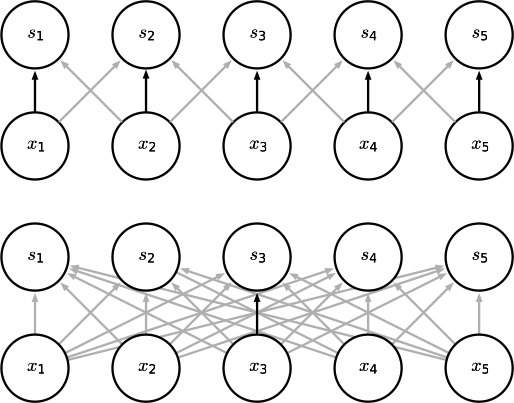
\includegraphics[width=0.5\textwidth]{./Images/shared_weights.png} }
  \caption[Shared weights.]{Shared weights~\cite{goodfellow2016}.}
\label{fig:shared_weights}
\end{figure}

The final output activations of a convolutional layer are computed in subsequent stages:
\begin{enumerate}
  \item linear unit activations are computed via the convolution operation,
  \item a nonlinear activation function is applied to the activations,
  \item a spatial subsampling (pooling) operation is applied.
\end{enumerate}

The rationale behind applying a nonlinearity is it makes the network capable of modelling nonlinear functions. Common activation functions include rectified linear $\max(0,x)$, sigmoid $\frac{1}{1+\exp(-x)}$, hyperbolic tangent $\tanh$, and many others. They have varying properties making them useful in different situations. We will not explore them further here.

\emph{Pooling} operation splits the neural units into sets of multiple adjacent activations and computes a summary statistic, such as the maximum element (max pooling) or the average (average pooling), per such set and outputs the result. If the stride between the sets is greater than one, the spatial dimension of output is decreased relative to input (subsampling).

The purpose of spatial subsampling is to ensure scale and distortion invariance by reducing the precision at which a feature is encoded in a feature map by reducing its resolution - when scale and distortion invariance is assumed, the exact location of a feature becomes less important and is allowed to exhibit slight positional variance - roughly speaking, an ``approximate'' translation invariance.

Although the combination of convolution and pooling performs well in many practical situations, it has multiple drawbacks. For example, the learned representations are not rotation invariant and thus, to mitigate this, the capacity of the network has to be increased and the training dataset must be enhanced to contain examples of rotated features, often extending the amount of data necessary and training time. A number of alternative approaches were suggested in the litarature.\footnote{For instance, Hinton's \emph{CapsNet}, described in~\cite{sabour2017}, is an attempt to transform the manifold of images of similar shape (which is highly nonlinear in the space of pixel intensities) to a space where it is globally linear by the way of using so called capsules instead of traditional convolutional layers.} For another example of a limitation, see Figure~\ref{fig:drawbacks}.

\begin{figure} 
\centering
\noindent\makebox[\textwidth]{%
  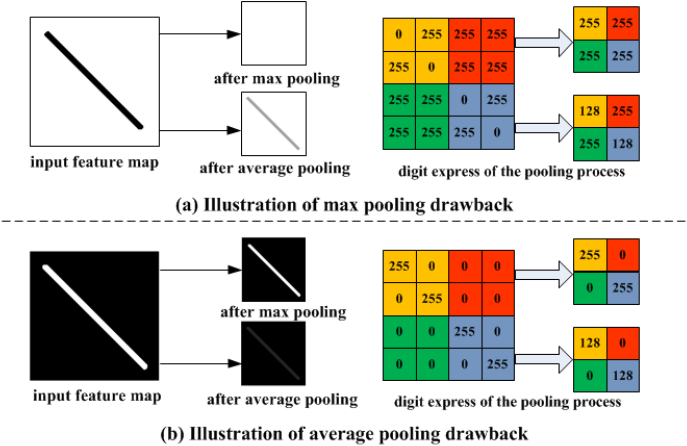
\includegraphics[width=0.8\textwidth]{./Images/drawbacks.png} }
  \caption[Drawbacks of pooling operation.]{Examples of drawbacks of the pooling operation. Max pooling discards all except the maximum element, and valuable information may thus be lost. Average pooling considers all the values, and the information about their contrast is reduced. Moreover, extreme values may have undesired effects on the result~\cite{yu2014}.}
\label{fig:drawbacks}
\end{figure}

\section{Common Spatial Patterns}
The method of Common Spatial Patterns (CSP) was originally proposed for people with impeded motor control (e.g. disabled people) in context of brain-computer interfaces, and thus most studies focus on its use in classification of motion performed or visualized by the subject. In our study, we will apply convolutional neural network architectures inspired by Filter Bank Common Spatial Patterns (FBCSP, see Section~\ref{sec:fbcsp}) for depression diagnosis and prediction of future remission of the disease.

As mentioned repeatedly in the previous text, the task of finding patterns in EEG signal associated with particular mind state or motor action present us with numerous challenges. CSP, and FBCSP in particular, are methods devised in attempt to overcome mainly two of them. Firstly, information about different temporally overlapping brain activities is conveyed in parallel in multiple frequency bands. For example, resting wakeful state comprises distinct idle rhythms over different cortical areas (such as $\alpha$-rhythm characteristic of idling visual cortex in the occipital area), which are overlapping with $\mu$-rhythms produced in sensorimotor areas both during imagined and performed movement. Secondly, the spatial origin of those signals is important for associating them with said mind states or motor actions. For example, different parts of the sensorimotor cortex over the central sulcus map directly to movements of distinct bodyparts. This is further complicated by the fact that EEG apparatus has inherently low spatial resolution due to small number of electrodes and poor volume conduction. 

Spatial filtering, then, is process of addressing this second challenge by accentuating signals from some areas, while attenuating others. And CSP analysis is a data-driven approach of achieving this by mutually maximizing the variance of spatially filtered signal associated with one activity, while minimizing the variance of filtered signal associated with other activity, thus making the signals independent (as Gaussian random processes)~\cite{blankertz2008optimizing}. In the following section, we will explain the process in detail.

\subsection{Algorithm} \label{sec:csp}
Let $C$ be the number of channels, and $\mathbf{x}(t) \in \RR^C$ be a band-passed, de-meaned and scaled multichannel EEG recording. CSP analysis yields a projection of $\mathbf{x}(t)$ of the signal from the original signal space to $\mathbf{x}_{\text{CSP}}(t) \in \RR^C$ by finding a matrix $W \in \RR^{C \times C}$, where
\begin{align*}
  \mathbf{x}_{\text{CSP}}(t) = W^T \mathbf{x}(t).
\end{align*}
Each column vector of $W$ is referred to as spatial filter. Thus, CSP decomposes the original signals into additive subcomponents, column vectors of $A \coloneqq (W^{-1})^T$, referred to as spatial patterns, giving name to the technique.

The matrix $W$ is found under optimization criteria, which we will describe in the following text. Firstly, let $\Sigma^{(+)} \in \RR^C$ and $\Sigma^{(-)} \in \RR^C$ be estimates of the inter-channel covariance matrices, corresponding to signals recorded in the two conditions $c$ we aim to distinguish, $+$ and $-$:
\begin{align*}
  \Sigma^{(c)} = \frac{1}{|I_c|} \sum_{i \in I_c} X_i X_i^{T}, \qquad c \in \{ +, - \},
\end{align*}
where $I_c$ is the set of time indeces matching the two conditions.\footnote{Here we suppose that two separate events happened during a single recording to simplify notation.} Since variance of band-pass filtered is the power present in the frequency band, the diagonal elements of $\Sigma^{(c)}$ represent the fraction of the total band power in each channel, and the off-diagonal elements represent the fractional covariance~\cite{koles1990spatial}. CSP then performs simultaneous decomposition 
\begin{align*}
  W^T \Sigma^{(+)} W &= \Lambda^{(+)}, \\
  W^T \Sigma^{(-)} W &= \Lambda^{(-)}, \qquad \Lambda^{(c)} \, \text{diagonal}
\end{align*}
under the condition that $\Lambda^{(+)} + \Lambda^{(+)} = I$, which is equivalent to solving the generalized eigenvalue problem
\begin{align*}
  \Sigma^{(+)}\mathbf{w} = \lambda \Sigma^{(-)}\mathbf{w}
\end{align*}
for generalized eigenvectors $\mathbf{w}$ and their eigenvalues $\lambda$. The resulting eigenvectors $\mathbf{w}_j$, $j \in \{1, \dots, C \}$ then are the column vectors of $W$, and corresponding eigenvalues $\lambda_j^{(c)} = \mathbf{w}_j^T \Sigma^{(c)} \mathbf{w}_j$ are the diagonal elements of $\Lambda^{(c)}$. Then, $\lambda_j = \lambda_j^{(+)} / \lambda_j^{(-)}$, and $\lambda_j^{(+)} + \lambda_j^{(-)} = 1$. This means that high variance in the direction of $\mathbf{w}_j$ of signal in class $+$ results in small variance in signal in class $-$, and vice versa (see Figure~\ref{fig:csp})~\cite{blankertz2008optimizing}.

This method, although loosely based on PCA, is better suited for supervised classification, since, unlike PCA, it is guaranteed to find components which are responsible for the maximum differences in variance between the two classes. These eigenvectors are an orthonormal set which spans $\RR^C$, and are optimal for the amount of variance they account for in the least squares sense~\cite{koles1990spatial}.

\begin{figure} 
\centering
\noindent\makebox[\textwidth]{%
  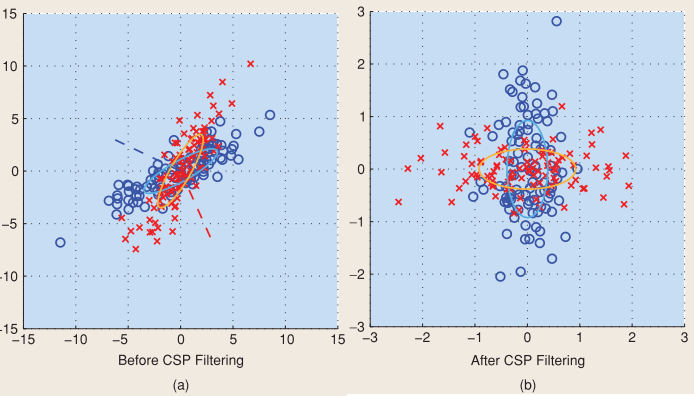
\includegraphics[width=0.7\textwidth]{./Images/csp/csp_merged.png} }
  \caption[Example of CSP algorithm.]{A demonstration of the CSP algorithm on a two classes of 2-dimensional samples generated randomly using different distributions~\cite{blankertz2008optimizing}. The dashed lines on the right hand side correspond to the CSP projection vectors $w_1$, $w_2$. Note that although there is a strong correlation for both classes in the original space, correlation for one class is maximized and and minimized for the other class in the projected space.}
\label{fig:csp}
\end{figure}

\subsection{Filter Bank Common Spatial Patterns} \label{sec:fbcsp}
Although CSP usually yields good performance when the signals have been filtered in frequency range carefully tuned for the particular subject and classification problem at hand, its performance rapidly decreases when measurements are either unfiltered or filtered in inappropriate frequency range~\cite{ang2008filter}. Thus, an improvement has been suggested, called Filter Bank Spatial Patterns (FBCSP). It comprises of four stages: frequency filtering, spatial filtering, feature selection and classification (see Figure~\ref{fig:fbcsp}). In stage 1, multiple band-pass filters are applied to split the signal into distanct filter banks. Then, in Stage 2, spatial filters are found for each of the respective filter banks using CSP analysis, as described in Section~\ref{sec:csp}. These filters characterize features present in the signal specific to the corresponding frequency band. In stage 3, a feature selection algorithm is employed to select the most discriminative features of all the filters found in previous step. Finally, in stage 4, a classification algorithm uses the selected features for classiying the input signal into a class.

Using the fact that magnitudes of the CSP eigenvalues are proportional to the amount of variance explained by corresponding signal in the direction corresponding to the eigenvector, the CSP algorithm in stage 2 is slightly modified to order the eigenvectors according to the magnitude of their eigenvalues, and only the first and last $m$ filtered signals are selected for further classification. This means selecting only the first and last $m$ rows from the matrix $X_{\text{CSP} = W^TX}$, yielding a matrix $Z \in (2m) \times T$ with row vectors $Z_j$, $j=1, \dots, 2m$. The final feature vector $\mathbf{f}$ is composed as logarithm of the contribution of variance of each row vector to the total variance as follows:~\cite{ang2008filter}

\begin{align} \label{eq:logvar}
  f_j = \log \left( \frac{\text{var}(Z_j)}{\sum_{i=1}^{2m} \text{var}(Z_i)} \right).
\end{align}

\begin{figure} 
\centering
\noindent\makebox[\textwidth]{%
  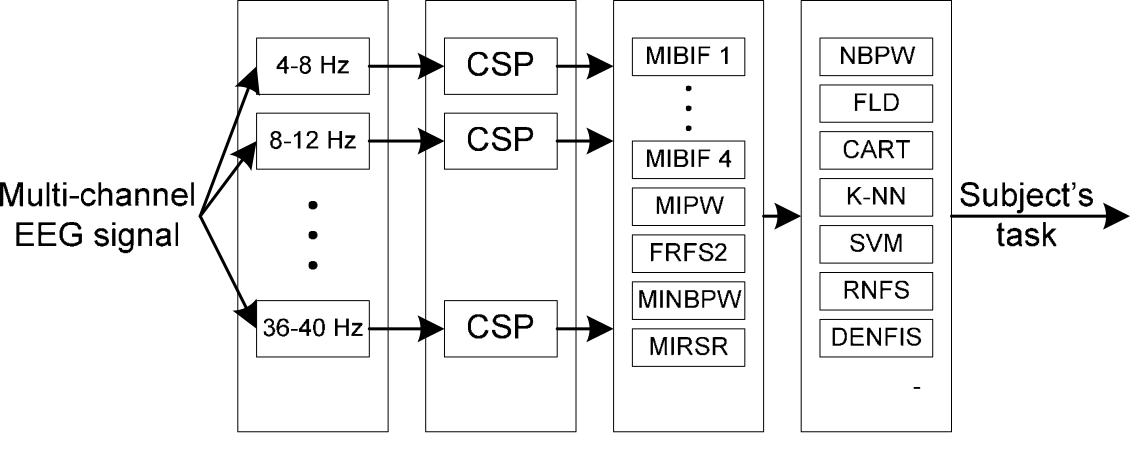
\includegraphics[width=0.8\textwidth]{./Images/fbcsp.png} }
  \caption[Schema of FBCSP algorithm.]{A schematic overview of the FBCSP~\cite{ang2008filter}. First, the signal is filtered into various bands. Then, CSP algorithm is applied to each band, and thus can maximize variance for class-specific features present in each band. After selecting features from subset of the signals, a classifier uses the features from all bands to perform the classification task.}
\label{fig:fbcsp}
\end{figure}

\section{Dataset} \label{sec:dl-dataset}
For experiments in this chapter, we used the same dataset as in the previous Chapter 1, described in Section~\ref{sec:dataset}. However, to increase the number of samples, decided to use the entire recordings, in contrast to our approach in the previous chapter, where we used only the beginning in each recording. This is mainly because the classification algorithms we used in this chapter have larger variance, and thus are easily overfit on small datasets. Thus, each of the recordings, after downsampling to $250$ Hz (see Section~\ref{sec:dataset}) was segmented into disjoint subrecordings of length 256, each subrecording forming a data sample. The subrecording length was selected as a tradeoff between 
\begin{itemize}
  \item the number of obtained samples,
  \item the amount of information contained withing each sample, and
  \item the size of data batch transferred to the GPU as input to the CNN.
\end{itemize}

As we will see in Section~\ref{sec:input-repr}, we decided to represent the input to the CNNs either as image-encoded signal, where the resulting size of the input is $O(N^2)$ for subrecording length $N$, or using raw data, where the input size is $O(C \times N)$ for constant number of selected channels $C$. Thus, the raw data input representation allows for longer subrecording length for the same data batch size compared to the image-encoded signal representation. However, we decided to use the same subrecording length for both input representations in order to make the results comparable. For the raw data, we did separate experiments increasing the length to 512 or 1024 using overlapping windows to keep the resulting number of samples constant, and obtained similar performance.

For the selected sampling frequency, this subrecording length corresponds to approximately a second of recording, which was shown to contain enough information to identify individuals with satisfactory accuracy using CNNs~\cite{ma2015resting}. Moreover, memory operations on data batches power of two bytes in size are easier to coalesce among multiple threads, thus improving runtime~\cite{goodfellow2016}. Finally, the reason for keeping the subrecordings disjoint was to minimize the amount of correlation between the samples.


After splitting the recordings, we assigned positive, neutral or negative label to each subrecording in order to split the dataset into three groups based on depression score of the subject at the time of the recording for depression classification, or based on the subject's before to after treatment depression score for response classification (in which case only before treatment recordings were further used). The neutral class was then removed and not further considered. 

The threshold values separating these classes were selected such that the classes remained relatively balanced and that enough samples were present in each class to train and evaluate a model of moderate capacity. In the case of depression classification, the amount of inter-class variance is inherently limited by nature of the provided data - patients were not randomly sampled, but visited the institution to seek professional help. In attempt to partially remedy this issue, the depression score threshold was set such that 71 patients remained in each depressed and healthy classes, leaving 124 neutral subjects. This corresponds to depression score ranges $\langle 0, 17 \rangle $ for healthy, $(17, 27)$ for neutral, and $\langle 27, 34 \rangle$ for depressed. In the case of response classification, our ability to potentially increase inter-class variance in this way is more limited due the amount of available data, since only before treatment recordings are used. Thus, we removed only 14 neutral subjects, leaving 59 nonresponding and 60 responding subjects.

\section{Input Representation} \label{sec:input-repr}
Before applying any machine learning technique to the classification problem at hand, the question of optimal input representation needs to be answered. To this end, multiple factors need to be considered. Firstly, what is the dimensionality of the input relative to the resulting number of samples, and does it allow construction of sufficiently complex architectures compared to complexity of the classification problem? Secondly, does each input sample contain enough information to perform successful classification? Thirdly, is the input representation appropriate for the kind of data, i.e. does it help or hinder successful classification? In our case, for all the methods considered, answer to the first question is a function of recording slice length used to generate the input. Answering the remaining questions, however, is difficult without prior experiments on similar datasets. For this reason, research on applying known techniques to new problems is useful.

Since well designed neural networks are characteristically able to learn feature maps given enough data, one obvious possibility is to use raw data. This approach has multiple benefits. First one, as we will see, is relatively low dimensionality. Global, and local features, no prior bias. Our first choice, then, was then to segment each recording into subrecordings of fixed length $l=256$, and, for each subrecording, order all its $C=19$ channels into rows of a $C \times l$ matrix. These matrices were then used as input samples. 

To use the results from the previous chapter, we also evaluated the models using only subsets of all the available electrodes. Those subsets were selected from the electrodes in which the mean values of nonlinear measures in Section~\ref{sec:distanal} were shown to be significantly different between studied groups, or which were selected during the feature selection step in~\ref{sec:results-nl}. However, we found either no notable improvements in performance, or slight deterioration of improvements.

As mentioned in Chapter 1, we consider the brain to be a nonlinear dynamical system. Another possibility, therefore, is to represent the input data as recurrence plots, which have considerable potential for representing properties of the dynamical system, as mentioned in Section~\ref{sec:recplot}. The obvious drawbacks are redundancy due to symmetry and high dimensionality, which is quadratic in the trajectory length. On the other hand, recurrence plots are known to capture properties of the system which are difficult to obtain using other methods in some cases~\cite{eckmann1987}. Morever, they have already been applied with success to classification of physical activites using convolutional neural networks~\cite{garcia2018classification}, and even some qualitative differences in recurrence plots have been observed between depressed and healthy patients~\cite{acharya2015computer}. We have discussed more applications in~\ref{sec:applications}.

For our computation of recurrence matrices, we used the Chebyshev norm. Chebyshev norm has multiple benefits, such as relatively low computational cost and distances independent of embedding dimension. Moreover, we observed subtler patterns on matrices computed using Chebyshev norm as opposed to those computed using Euclidean $L_2$ norm. For comparison, see Figure~\ref{fig:norm-comp}.

Our last method of input representation is inspired by success of Gramian Angular Fields (GAFs) for sequence classification~\cite{wang2015imaging} using convolutional neural networks. To obtain GAF matrix from a scalar time series $x_1, x_2, \dots, x_N$, one first scales the time series into interval $(-1, 1)$, and then each value $x_i$ of the time series is converted into complex number with mode and radius given as
\begin{align*}
\phi_i &= \arccos (x_i), \\
r_i &= i/N.
\end{align*}
This way, temporal dependencies are conserved through the radius. Then, instead of scalar product, an operation $\oplus$ is defined as
\begin{align*}
  x_i \oplus x_j = \cos(\phi_i + \phi_j)
\end{align*}
and a quasi-Gram $NxN$ matrix $G$ is computed as
\begin{align*}
  G = \begin{pmatrix}
      \cos(\phi_1 + \phi_1)  & \cos(\phi_1 + \phi_2) & \dots & \cos(\phi_1 + \phi_N) \\
      \cos(\phi_2 + \phi_1)  & \cos(\phi_2 + \phi_2) &  \dots & \cos(\phi_2 + \phi_N)  \\
      \vdots & \vdots & \dots & \vdots \\
      \cos(\phi_N + \phi_1)  & \cos(\phi_N + \phi_2)  & \dots & \cos(\phi_N + \phi_N)
     \end{pmatrix}.
\end{align*}

Since GAFs which are defined only for single channel time series, we modify this approach, use spatial embedding, thus obtaining a multi-channel time series $\mathbf{x}_1, \mathbf{x}_2,\dots, \mathbf{x}_N$, and then compute cosine similarities between each pair of those vectors as
\begin{align*}
  G = \begin{pmatrix}
    \frac{\mathbf{x}_1 \cdot \mathbf{x}_1}{\norm{\mathbf{x}_1} \norm{\mathbf{x}_1}} & \frac{\mathbf{x}_1 \cdot \mathbf{x}_2}{\norm{\mathbf{x}_1} \norm{\mathbf{x}_2}} & \dots & \frac{\mathbf{x}_1 \cdot \mathbf{x}_N}{\norm{\mathbf{x}_1} \norm{\mathbf{x}_N}} \\
    \frac{\mathbf{x}_2 \cdot \mathbf{x}_1}{\norm{\mathbf{x}_2} \norm{\mathbf{x}_1}} & \frac{\mathbf{x}_2 \cdot \mathbf{x}_2}{\norm{\mathbf{x}_2} \norm{\mathbf{x}_2}} & \dots & \frac{\mathbf{x}_2 \cdot \mathbf{x}_N}{\norm{\mathbf{x}_2} \norm{\mathbf{x}_N}} \\
    \vdots & \vdots & \dots & \vdots \\
    \frac{\mathbf{x}_N \cdot \mathbf{x}_1}{\norm{\mathbf{x}_N} \norm{\mathbf{x}_1}} & \frac{\mathbf{x}_N \cdot \mathbf{x}_2}{\norm{\mathbf{x}_N} \norm{\mathbf{x}_2}} & \dots & \frac{\mathbf{x}_N \cdot \mathbf{x}_N}{\norm{\mathbf{x}_N} \norm{\mathbf{x}_N}} \\
      \end{pmatrix}.
\end{align*}

Since both recurrence plot and cosine similarity matrix are symmetric, we applied the following procedure for computing them. For a given subseries length $l_s$, we computed recurrence plot of subseries $2l_s$, and considered only lower left quadrant. This way, the inherent redundancy was completely removed, while preserving some of the information - the lower left quadrant contains relationships (i.e. distances or similarities) between time states occuring in the previous subseries of length $l_s$. 

\begin{figure}
\centering
\begin{subfigure}{.5\textwidth}
  \centering
  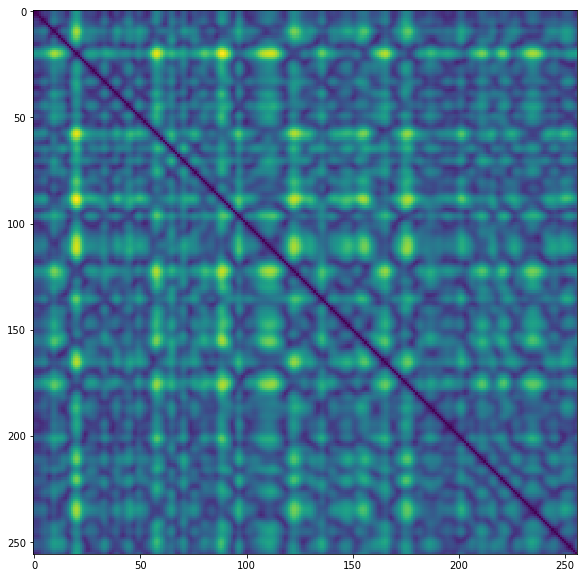
\includegraphics[width=.9\linewidth]{./Images/recplots/euclidean.png}
  \caption{Euclidean norm.}
  % \label{fig:sub1}
\end{subfigure}%
\begin{subfigure}{.5\textwidth}
  \centering
  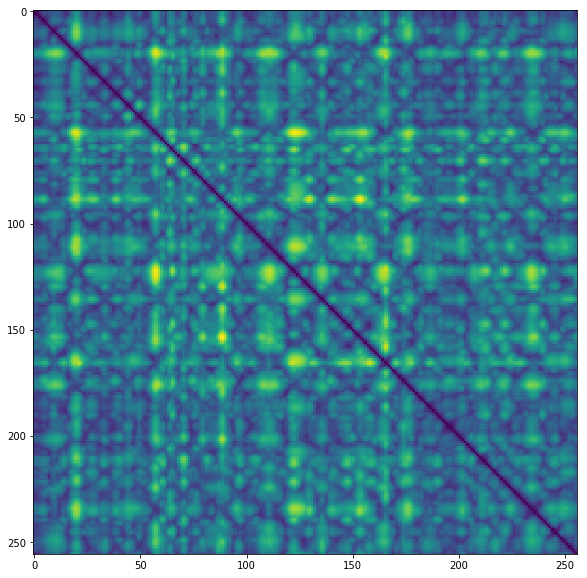
\includegraphics[width=.9\linewidth]{./Images/recplots/chebyshev.png}
  \caption{Chebyshev norm.}
  % \label{fig:sub2}
\end{subfigure}
\caption[Comparison of Euclidean and Chebyshev norms on RP.]{Recurrence plots computed using different norms. We can see that the figure on the right hand side has sligthly crisper patterns.}
\label{fig:norm-comp}
\end{figure}

\info[inline]{Another possibility is to learn on flattened scalp images of topographical distributions of different band powers. However, as explained in~\cite{schirrmeister2017deep}, this presents two main challanges. As we have verified in the previous chapter (see Section~\ref{sec:band-ampl}), the relevant variance is probably spatially global in nature, and not hierarchically compositional to make use of CNN. On the other hand, the temporal patterns are more likely to be hierarchically compositional.}

\section{Preprocessing} \label{sec:dl-preprocess}
% Preprocessing: Filtering, running average and standard deviation.
Signals were preprocessed before either image-encoding or direct classification. First, the electrode voltages were converted to mV to improve numerical stability. Then, optionally, a high-pass Butterworth filter of order 3 with 4 Hz cutoff frequency was applied. It has been suggested that in some cases, filtering the signals may improve classification performance. \add{Elaborate, cite, mayber refer to discussion in previous chapter.} In image-encoded case, the signals were encoded at this stage. Finally, Welford's algorithm for running mean and standard deviation was used to compute the mean and variance over the whole dataset, and the dataset was then centered and normalized according to the found values.

\section{Architecture} \label{sec:dl-arch}
Our choice of CNN architectures was heavily inspired by, and almost identical to, those used in~\cite{schirrmeister2017deep}. These architectures, and in particular the second one (in order of description below), were designed by the authors to be analogous to the FBCSP pipeline described in detail in Section~\ref{sec:csp}. 

The first architecture, called \emph{deep} (see Figure~\ref{fig:deep}), is more generic of the two architectures used, bearing resemblence to the architectures which proved successful in traditional computer vision tasks. It consists of four convolutional blocks with batch normalization ($\epsilon = 10^{-5}$, $\text{momentum} = 0.1$) and ELU nonlinearity, followed by max pooling and dropout ($p = 0.5$). The batch normalization was applied before the activation function. The convolution was performed only along the temporal dimension, with kernel size $(1,3)$, stride $1$. The pooling operation was also performed only along the temporal dimension, with kernel size $(1,3)$, stride $3$. For image input, we used traditional 2D convolution with kernel size $(3,3)$. The first convolutional layer is an exception - to explicitly seperate the linear transformation into combination of temporal and spatial convolution, this layer is split into two layers with no activation function in between. First, a temporal convolution with kernel size $(1,10)$ is performed, followed by a spatial convolution across all channels with kernel size $(19,1)$. Note that the first operation can be seen as analogue of band-pass filtering, and the second as spatial filtering, as performed by CSP algorithm, with the difference that the filters are ``constructed'' by gradient descent. Batch normalization and pooling operations are also performed as described above. 

The second architecture, called \emph{shallow} (see Figure~\ref{fig:shal}), is more specialized, tailored to mimic the transformations performed by the FBCSP pipeline. The first and only convolutional layer is split in the same way as in the deep architecture described above, and batch normalization is also applied before the activation. However, squaring nonlinearity was used as activation function for the layer instead, followed by average pooling. This can be seen as approximation of computing mean power. Moreover, following the recommendations mentioned in~\cite{schirrmeister2017deep}, larger kernel size $(1,25)$ is used for the temporal filtering in this network. Then, logarithm nonlinearity is applied, analogous to the mean log-variance computation in FBCSP, see (\ref{eq:logvar}). One of the advantages of this architecture over FBCSP that it can learn the structure of temporal changes in the representation of ``band-powers''.

In both deep and shallow architectures, the classification is performed by classification layer with 2D convolution of kernel size of the last layer, 2 filters, and logistic activation to produce probability estimate for each class. For optimization, we used stochastic gradient descent with Nesterov momentum $0.99$, decay $10^{-5}$, learning rate $0.01$ for batch size $128$ (which we used for raw data), and learning rate $0.001$ for batch size $64$ (which we used for image data due to hardware limitations). This last change was made because lower batch size leads to more updates per epoch.

We also attempted different configurations: increasing or decreasing the number of layers in the deep network, increasing or decreasing the kernel sizes, ReLU activation functions, and Adam or rmsprop optimizers. However, we found any of these changes leading to degradation in performance. 

For image-encoded data, i.e. recurrence plots and cosine similarities, we also tried the architecture (along with the same hyperparameters) used in~\cite{garcia2018classification}, which resulted in overall accuracy of 0.942 and 0.804 recall on classification task of 6 activies using recurrence plots and CNNs (as mentioned in Section~\ref{sec:applications}), evaluated using 10-fold cross validation on over 10 000 samples. However, we were unable to replicate the result. This may be because of the difference in input image sizes, number of used input channels - the authors had only 4 electrodes available, and used all of them as input channels, whereas we used spatial embedding (see Section~\ref{sec:embedding}).

Moreover, we also evaluated multiple simpler architectures. The best performing (both on image-encoded and raw data) was a VGG-like model with 3 convolution-pooling modules (convolution kernels $(3,3)$, pooling kernels $(2,2)$, ReLU activation functions) with 8, 16 and 16 filters respectively. These were followed by dropout ($p=0.5$), and fully connected sigmoid classification layer. This model, optimized by rmsprop, achieved $73\%$ accuracy on stand-out test set on raw data, and below $60\%$ on the image-encoded data. All attempts of modifying capacity and regularization, i.e. adding batch normalization, adding or removing layers, increasing or decreasing the number of filters, as well as adding weight normalization or changing the optimizer, lead to deterioration of performance.

\begin{figure}
\centering
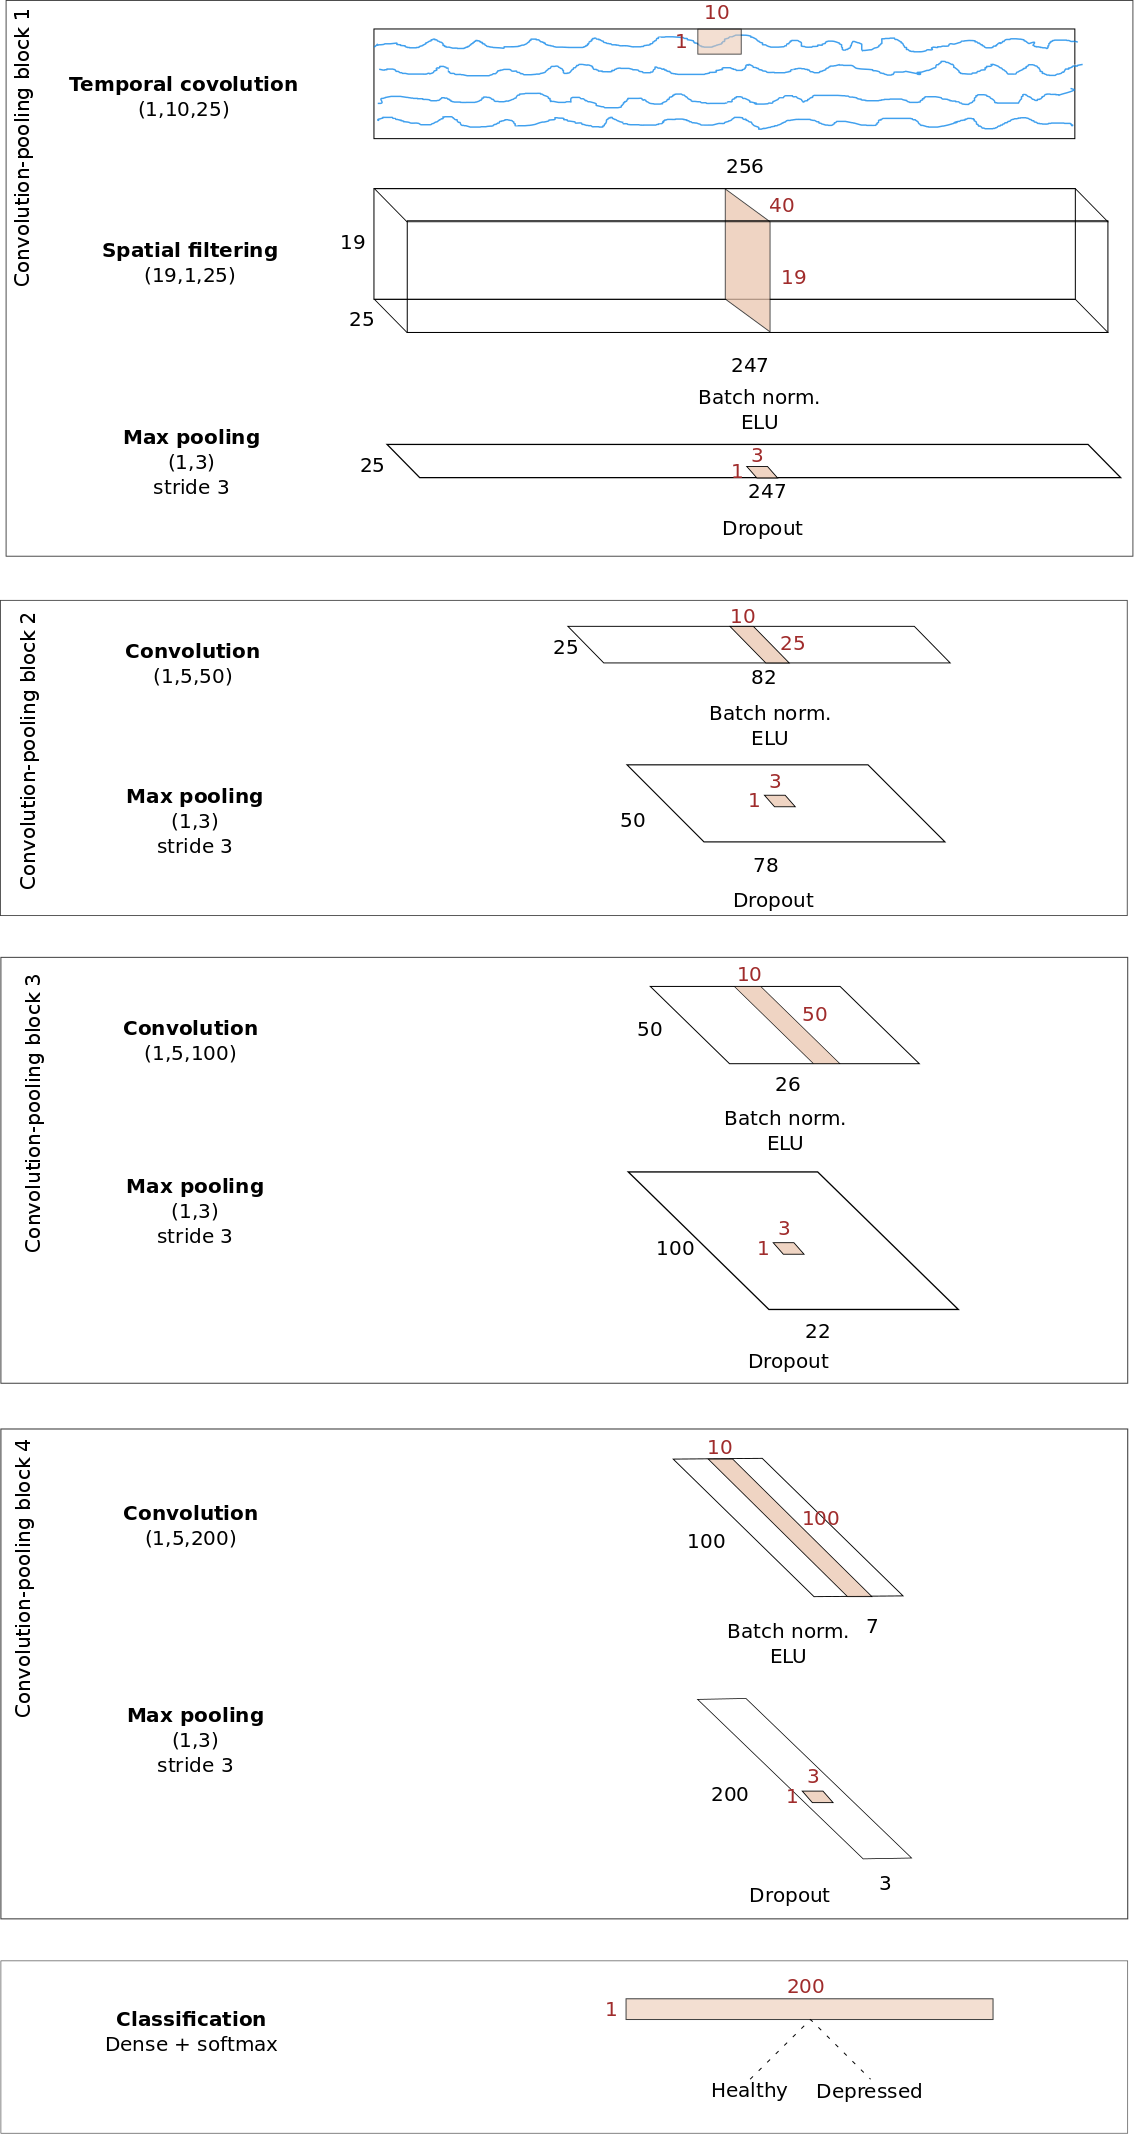
\includegraphics[width=0.7\linewidth]{./Images/archs/deep.png}
\caption[Deep architecture diagram.]{Deep architecture for evaluation on the raw data. For evaluation on image-encoded data, the kernel sizes were changed - see text for details.}
\label{fig:deep}
\end{figure}

\begin{figure}
\centering
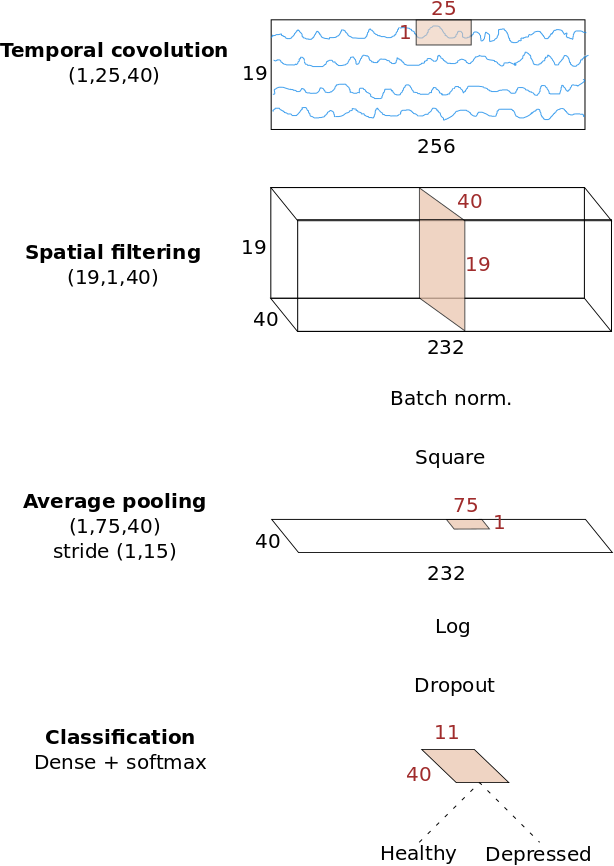
\includegraphics[width=.7\linewidth]{./Images/archs/shal.png}
\caption[Shallow architecture diagram.]{Shallow architecture, inspired by FBCSP algorithm, which achieved outstanding performance on the raw data.}
\label{fig:shal}
\end{figure}

\section{Results} \label{sec:dl-results}
\subsection{Methodology}
In order to train and evaluate the models, we used 5-fold cross validation performed as follows. Before training and evaluation the models, all the samples were shuffled and split into two parts. The first part, containing 80\% of the samples, was used for training (80\%) and validation (20\%). The second part, containing the remaining 20\% of the samples, was used as test set to evaluate the trained model. This procedure was again performed 5 times, using different initial splits into training with validation and test set. The results in Table~\ref{tab:dl-res} report the mean and standard deviation of accuracies obtained on the test sets. Figure~\ref{fig:acc-loss-orig} shows evolution of the accuracy and loss of the shallow model on the depression classification task during one cross validation cycle.

The models were trained for 200 epochs. In each epoch, the current iteration of the model was evaluated on the validation set. The model which achieved the highest accuracy on the validation set over all iterations was then selected for evaluation on the test set. This procedure, performed on the dataset described in Section~\ref{sec:dl-dataset}, results approximately in the number of samples for each of training, validation and test sets shown in Table~\ref{tab:setsize}.

In Table~\ref{tab:dl-res}, where we use SHAL to denote the shallow architecture and DEEP to denote the deep architecture (see Section~\ref{sec:dl-arch}). The unfiltered input is denoted $0-f_{\text{fin}}$, and $4-f_{\text{fin}}$ signifies that high pass filter with cutoff frequency of $4$ Hz was applied to the input (see Section~\ref{sec:dl-preprocess}). Firstly, the shallow architecture performs noticeably better on the prognosis task than the deep architecture. Secondly, filtering has not much effect, but seems to improve the results slightly for the prognosis task, but does not help on the diagnosis task. Finally, although it was suggested in~\cite{acharya2015computer} that recurrence plots \dots and GAFs were shown to improve time series classification~\cite{wang2015imaging}, both recurrence plots and cosine similarities do not seem to be effective encoding techniques for convolutional neural networks we evaluated on this dataset.

% Conclusions: SHAL has state of the art performance on RES. It would be nice to evaluate against pure FBCSP, and try more traditional configuration to see difference in performance. Combination of CNN and recurrence plots is likely not especially effective.

\begin{table}[tbp]
\centering
\begin{tabular}{|c|c|c|c|c|}
\hline
\textbf{Dataset} & \multicolumn{2}{c}{\textbf{DEP}} \vline & \multicolumn{2}{c}{\textbf{RES}} \vline \\ \hline
& \textbf{Neg.} & \textbf{Pos.} & \textbf{Neg.} & \textbf{Pos.} \\ \hline
Training & 3278 & 3230 & 2684 & 2705 \\ \hline 
Validation & 826 & 802 & 686 & 662 \\ \hline 
Test & 1038 & 997 & 830 & 855 \\ \hline 
Overall & 5142 & 5029 & 4200 & 4222 \\ \hline 
\end{tabular}
\caption[Training, validation, and test set sizes.]{Number of negative / positive samples in training, validation, test sets.}
\label{tab:setsize}
\end{table}

\begin{table}[tbp]
\centering
  \parbox{.49\linewidth}{
\centering
\begin{tabular}{|c|c|c|c|c|}
\hline
\textbf{Label} & \textbf{Freq.} & \textbf{Arch.} & \multicolumn{2}{c}{\textbf{Accuracy}} \vline \\ \hline
& & & \textbf{Mean} & \textbf{Std} \\ \hline
\multirow{4}{*}{DEP} & $0-f_{\text{fin}}$ & SHAL &  $0.85$ & $0.13$    \\ \cline{2-5}
                     & $4-f_{\text{fin}}$ & SHAL &     $0.84$ & $0.11$    \\ \cline{2-5} 
                     & $0-f_{\text{fin}}$ & DEEP &     $\mathbf{0.86}$ & $0.01$    \\ \cline{2-5} 
                     & $4-f_{\text{fin}}$ & DEEP &     $0.85$ & $0.02$    \\ \hline
\multirow{4}{*}{RES} & $0-f_{\text{fin}}$ & SHAL &  $\mathbf{0.94}$ & $0.02$    \\ \cline{2-5} 
                     & $4-f_{\text{fin}}$ & SHAL &     $0.94$ & $0.03$    \\ \cline{2-5} 
                     & $0-f_{\text{fin}}$ & DEEP &     $0.88$ & $0.01$    \\ \cline{2-5} 
                     & $4-f_{\text{fin}}$ & DEEP &     $0.86$ & $0.02$    \\ \hline
\end{tabular}
\subcaption{Raw data.}
% \label{tab:depcl}
}
\hfill
  \parbox{.49\linewidth}{
\centering
\begin{tabular}{|c|c|c|c|c|}
\hline
\textbf{Label} & \textbf{Freq.} & \textbf{Meth.} & \multicolumn{2}{c}{\textbf{Accuracy}} \vline \\ \hline
& & & \textbf{Mean} & \textbf{Std} \\ \hline
\multirow{4}{*}{DEP} & $0-f_{\text{fin}}$ & RP &   $\mathbf{0.63}$ & $0.02$ \\ \cline{2-5}      
                     & $4-f_{\text{fin}}$ & RP &      $0.61$ & $0.01$   \\ \cline{2-5}             
                     & $0-f_{\text{fin}}$ & CS &      $0.59$ & $0.02$  \\ \cline{2-5}              
                     & $4-f_{\text{fin}}$ & CS &      $0.58$ & $0.01$ \\ \hline
\multirow{4}{*}{RES} & $0-f_{\text{fin}}$ & RP &   $0.61$ & $0.03$ \\ \cline{2-5}               
                     & $4-f_{\text{fin}}$ & RP &       $\mathbf{0.65}$ & $0.02$    \\ \cline{2-5}   
                     & $0-f_{\text{fin}}$ & CS &      $0.55$ & $0.02$ \\ \cline{2-5}               
                     & $4-f_{\text{fin}}$ & CS &      $0.63$ & $0.01$ \\ \hline               
\end{tabular}
\subcaption{Image-encoded data.}
% \label{tab:depcl}
}
\caption[Evaluation of CNN architectures.]{Evaluation of accuracies of the shallow (SHAL) and deep (DEEP) architectures on the raw and image-encoded data in classification of depression state (DEP) or prediction of response (RES).}
\label{tab:dl-res}
\end{table}

\begin{figure}
  \centering
  \includegraphics[width=1.0\linewidth]{./Images/acc_loss_orig_dep_all_nonfilt.png}
  \caption[Accuracy and loss for the original splitting.]{An example of accuracy and loss measured on the validation and test set during one cross validation cycle for the shallow network on the depression classification task.}
  \label{fig:acc-loss-orig}
\end{figure}

\add[inline]{We might want to show the missclasifications - how close were they? Are people acting, or is the measurement relatively objective? Or maybe confusing matrices.}
\add[inline]{How about seeing hidden layer activations typical of particular class?}
\info[inline]{Batchsize 64 128 doesn't matter. The learning rate was decreased with batch size.}
\info[inline]{CHanges to number of any parameter, including adding layers made the results worse. Interestingly, simpler models overfit the training set very quickly, and regularization hurt performance. Hence, this model is probably at least close to local optima in hyperparameter space.}
\info[inline]{Maybe measure shallow model with more traditional activations to see how much performance is due to FCP.}

\subsection{Limitations} \label{sec:dl-limit}
As evidenced in Section~\ref{sec:analbefaft}, nonlinear measures seem to be relatively stable over time for individual patients. Moreover, it has been observed that EEG signals contain other temporally stable patterns which can be used for individual identification~\cite{}. Since the method we used for training and evaluation described in Section~\ref{sec:dl-results} involved cross validation over samples instead of patients, the test set includes distinct samples from the same patients. This raises the question whether the models indeed learn to identify the patterns contributing to the label, or whether instead they learn to identify the patterns associated with the patients, and thus they infer the label indirectly.

To investigate this question, we trained and evaluated the models as follows. The patients were split into two sets. The first set was again used for training and validation and containing 80\% of the patients, and the second set, containing the remaing samples, was used for testing. Only either the recordings obtained during the first visit, or recordings obtained during the second visit, were used (this required changing the depression score thresholds to keep the classes balanced). This way, samples from patients used in the test set were never used for training. The first set was then split into training (80\%) and validation (20\%) sets of distinct patients, and the model was trained and evaluated on samples obtained from these distinct patients using the method described in Section~\ref{sec:dl-results}. This entire procedure was repeated 5 times, resulting in 5-fold cross validation across patients.

Figure~\ref{fig:acc-loss-fixed} shows loss and accuracy on the training and validation sets during one loop of the cross validation using the simpler, shallow model on the recordings obtained during the first session to predict the depression score level. In order to maximize the amount of training data, the thresholds for the classes were set to 26 as upper bound for healthy and 27 as lower bound for depressed, resulting in 63 and 62 patients in each group respectively. The figure shows that the model fits the training set of small number of patients, but does not generalize to the patients the patients in the validation set. Thus, the number of training epochs before evaluation on test set was decreased. Increasing the probability parameter of dropout, adding regularization to the layers, increasing or shortening the recording length to either increase the amount of information in a sample or simplify the model, or increasing the overlap between samples and shifting more patients to the training set does not improve generalization. Table~\ref{tab:res-pat-split} shows accuracies obtained using this procedure with varying subrecording length and width.

We also changed the evaluation strategy on the test set to report percentage of successfully classified patients, where each patient was successfully classified if the majority of samples corresponding to the patient's recording was correctly classified. However, the resulting accuracies were similar to the accuracy obtained per sample. This means that the false predictions were evenly distributed across patients.

\begin{figure}
\centering
\includegraphics[width=1.0\linewidth]{./Images/acc_loss_fixed.png}
\caption[Accuracy and loss for modified splitting.]{The accuracy and loss obtained for the depression classification task on training and validation sets split across patients. Only recordings acquired during the first session were used, and thus samples in each of training, validation and test sets were acquired from distinct patients. The subrecordings were non-overlapping, and the subrecording length was 256, equal to the subrecording length used for evaluation in Section~\ref{sec:dl-results}. We can see that the model overfits the training set during the initial epochs, and fails to generalize to the validation set.}
\label{fig:acc-loss-fixed}
\end{figure}

% The evaluation could be done by: average per person. Is not efficient on small number of persons.

\begin{table}[tbp]
\centering
\begin{tabular}{|c|c|c|c|c|c|c|c|}
\hline
\multicolumn{2}{|c|}{\textbf{Subrecording}} & \multicolumn{3}{|c|}{\textbf{Dataset sizes}} & \multicolumn{2}{|c|}{\textbf{Accuracy}} \\ \hline
\textbf{Length} & \textbf{Overlap}(\%) & \textbf{Train.} & \textbf{Val.} & \textbf{Test} & \textbf{Mean} & \textbf{Std}  \\ \hline
256 & 0 & 5277 & 1453 & 1785 & 0.55 & 0.02 \\ \hline
512 & 50 & 5202 & 1433 & 1759 & 0.57 & 0.03 \\ \hline
1024 & 25 & 5052 & 1295 & 1707 & 0.55 & 0.02 \\ \hline
% 1024 & 50 & 2538 & 702 & 861 & 0.57 & 0.06 \\ \hline
\end{tabular}
\caption[Accuracies obtained using cross validation across samples.]{Accuracy of the shallow model on the depression classification task using raw data representation of recordings obtained before treatment. The dataset contained 63 patients labeled as healthy (depression score below 26) and 62 patients labeled as depressed (depression score above 27).}
\label{tab:res-pat-split}
\end{table}

Another modification of the training procedure was evaluated. The split between training with validation and test was again performed across patients. However, the instead of splitting the training with validation set into training and validation sets across patients, we split it across samples. This way, we obtained good performance on the validation set. Nevertheless, the performance on the test set did not noticeably improve.

A possible explanation for the obsered result is as follows. It seems that the relatively high performance obtained in the previous section was mostly due to small intrapersonal variance and high interpersonal variance of the patterns in the EEG signals resulting in the network being trained to map patient-characteristic patterns to labels, instead of mapping label-characteristic patterns to labels. Hence, the models overfit over a small number of epochs to the training set of small number of patients, and is unable to generalize to another set of patients.

This hypothesis is supported by a considerable amount of research dedicated to finding subject specific traits in EEG~\cite{del2014electroencephalogram}. There is ample evidence that certain aspects of EEG morphology are phenotypic. In~\cite{}, the authors concluded that EEG of monozygotic twins are identical, whereas EEG of dizygotic twins show lesser degree of similarity. This result has been replicated multiple times and using various methods. Furthermore, alpha peak frequency and peak frequency in occipital regions seems strongly heritable~\cite{}. Since then, a number of EEG-based identity verification systems have been proposed~\cite{del2014electroencephalogram}.

If this hypothesis holds, then the observed lack of generalization may be improved by increasing the number of patients included in the dataset. Assuming that the dataset would then contain large enough aggregate of patients with small variance in patient-charecterstic patterns and, at the same time, high enough variance in depression scores and treatment response, large training accuracy could be achieved by fitting the label-characteristic patterns. Conceivably, models trained on such dataset would generalize to patients not included in the training set.

\section{Implementation}
For the implementation in this chapter, we used the same software as in Chapter~\ref{ch:nonlin-approach}, which was listed in Section~\ref{sec:impl-nl}. In additition, to design and evaluate the models, we used the deep learning library \href{https://keras.io/}{Keras}.

\chapter*{Conclusion} \label{ch:concl}
\addcontentsline{toc}{chapter}{Conclusion}
In this study, we incorporate both thorough review of the theory of nonlinear dynamical systems in relation to EEG analysis along with overview of the relevant algorithms and techniques for nonlinear measures extraction and input parameter estimation, comprehensive literature review, and practical application of those techniques on an original dataset. Furthermore, we develop and evaluate an approach to the same task based on multilayer convolutional neural networks and objective function optimization using iterative optimization.

\section*{Contributions}
\subsection*{Analysis of Correlation between Depression Score and Nonlinear Measures}
Investigating the significance of correlations between nonlinear measures and depression scores, we found that LLE, DFA, HE, HD, and SE computed from EEG signals recorded from channels near certain cortical areas are significantly correlated with depression score. The most statistically significant correlations were found for LLE, which, was found as least discriminative in a similar experimental setting \cite{hosseinifard2013}. Although CD showed no significant correlations with depression score per channel, using it in combination with other nonlinear measures or by combining a number of channels resulted in one of the most accurate depression classifiers evaluated. Out of the feature selection algorithms used for selection of the most discriminative measures and channels, genetic algorithm was shown to be the most effective. 

All the studies reviewed in Section~\ref{sec:applications} included a control group of symptomless, clinically healthy patients, whereas our dataset consists exclusively of patients suffering from MDD of various symptom severity. Nevertheless, the accuracies achieved by the classifiers are substantial, indicating possible relationship between depression severity and values of nonlinear measures recorded in EEG signals obtained from various cortical regions, and opening a possibility for developing a regression model predicting depression score making use of nonlinear measures.

\subsection*{Largest Lyapunov Exponents are Predictive of Positive Treatment Response}
As we outlined in Section~\ref{sec:applications-prog}, most of the EEG-based treatment outcome prediction has been focused on quantifying frontal $\theta$ band. This approach leans on strong neuroscientific support. In the analysis performed in Section~\ref{sec:analrespdif}, we found significant differences in distributions of LLE estimated from signals recorded in channels across multitude of cortical areas, especially near frontal (F3, F4) and left temporal (T6) areas. Almost no significant differences were found using other nonlinear measures. Interestingly, although LLE was positively correlated depression score, it is negatively correlated with treatment response. In other words, depressed patients exhibit slightly higher chaoticity than healthy patients (see Section~\ref{sec:analdepdif}), but out of those depressed patients, those with lower chaoticity at the beginning of the treatment may be more likely to respond positively to that treatment (see Section~\ref{sec:analrespdif}). However, note that~\cite{nandrino1994} observed higher predictability, and thus lower complexity in EEG signals of depressed patients using different methods.

Indeed, in Section~\ref{sec:nl-res-prog}, LLE was shown to be potent feature for treatment outcome prediction classifiers. These results may encourage further exploration of the potential use of nonlinear dynamical measures for treatment outcome prediction, which, to our knowledge, is nonexistent at present.

\subsection*{Analysis of Spatial Distribution of Nonlinear Measures across Brain Regions in Depression}
Although some neuroscientific theories suggest that medical depression is caused by malfuction in the right hemisphere~\cite{hecht2010depression, kwon1996right}, in Sections~\ref{sec:analdepdif} and~\ref{sec:results-nl}, we found nonlinear measures computed in both hemispheres contribute significantly to high depression score. The distributions of correlation significance is notably particular to each measure, possibly indicating that variously distributed and different processes captured by each measure contribute to depression severity. \add{Too speculative? Belongs more to discussion?}For example, DFA and HE show most significant correlations with depression score in right parietal regions, LLE and SE in right temporal regions,  Nevertheless, the most successful depression classifiers made use especially of channels in temporal areas (T6 in particular).

\subsection*{Analysis of Nonlinear Measure and Input Parameter Estimation Algorithms and Procedures for EEG Analysis}
Since computation of nonlinear measures requires laborious selection of input parameters and knowledge of the algorithms in order to interpret the results, these methods often remain inaccessible to practitioners who has not yet become experts in the field of nonlinear dynamical analysis~\cite{schmid1996indications}. Therefore, there is a need for automated procedures to ease application of these methods and increase their use and availability. For the purpose of computing LLE and CD, in Section~\ref{sec:estim-nl}, we evaluated a range of algorithms for estimation of embedding dimension and time delay parameters, including implementations of automated pipelines for computation of said measures. Although these input parameter estimation algorithms remain widely used (see Sections~\ref{sec:lle-rev} and~\ref{sec:corrdim-rev}), we found that, for our dataset, their outputs varied widely for each method, and provided only a crude approximation for parameters which produced more discriminative measures. One of the most consistent and informative estimation algorithms was ILD of our own implementation, which, however, suffers from relatively high computational costs.

\subsection*{Evaluation of FBCSP-inspired Neural Network Architectures for Depression Diagnosis and Prognosis}
In Section~\ref{sec:dl-results}, we evaluated two CNN architectures which were previously shown to be successfully applied to decoding task-related information~\cite{schirrmeister2017deep, schirrmeister2017deeppatho}. The models achieved relatively high accuracy when trained and evaluated using cross validation across samples. However, when trained and evaluated using cross validation across recordings obtained before treatment from individual, distinct patients, the models achieved only modest accuracy, and did not generalize to the test set (see Section~\ref{sec:dl-limit}). This observation may be explained by low intrapersonal, and high intrapersonal variance of the EEG signals, which results in high correlation of samples corresponding to one patient, and thus in the presence of high number of samples from small number of patients, the model is trained to associate labels to samples based on the patient-charecterstic patterns, instead of label-characteristic patterns. Indeed, a number of studies suggest presence of phenotypic traits in EEG, and personal identification using EEG is a flourishing field~\cite{del2014electroencephalogram} (see Section~\ref{sec:dl-limit}). If this hypothesis holds, then performance of these models may be improved by extending the dataset with enough patients with similar patient-characteritic patterns and different label-characteristic patterns. Such dataset may be obtained by tracking patients' depression score across extended time span.

% \section*{Limitations}
% \begin{itemize}
%   \item Correlation in CNN samples, also they are too short
%   \item Dataset lacks controls, imbalanced for remission
%   \item 50 Hz noise in some samples
%   \item Patients offered various treatment - e.g. it may be possible that response to rTMS may be different from response to drugs
%   \item Outputs only binary label, doctors may want more precise (e.g. 95\% confidence interval, but it is currently to large)
%   \item All NL measures correlated with depression scores, reasonable accuracy which is not as high as in other studies, but we have larger dataset than many. On the other hand, we lack control group (next Section).
% \end{itemize}

\section*{Recommendations for Future Work}
% \begin{itemize}
% \item Filter 50 Hz
% \item Try combining modalities
% \item New spatiotemporal NL measures (see Stam) - current are spatially local, temporally global
% \item Compare with FBCSP, with spatial embedding
% \end{itemize}

% Recommendations addressing limitations (filtering, dataset?)

% Conceptual recommendations (NL measures framework)

% Recommendations based on findings
% Neuroscientific understanding of observed correlations may improve techniques
% Explore NLD in prognosis, left temporal area
% Implement app

The nature of our dataset restricts us to analysis of patients suffering from depressive symptoms to varying degrees. Although obtaining accuracy lower in comparison with studies employing healthy, symptom-free group as well as depressed patients is justifiable, we believe that this accuracy can still be significantly improved with more advanced noise-reduction preprocessing techniques, and recording environment insulated from power-line, electronic devices, and other sources of electromagnetic interference. Moreover, the patients should be advised to keep their eyes closed, an ECG may recorded simulatenously and later used to remove interference from the heart muscle. Potentially, machine learning techniques may be used improve the signal quality by continuously estimating it, and even detecting events such as lost electrode contact~\cite{schirrmeister2017deep}.

Due to the fact that computing nonlinear dynamical measures on a nonstationary signal is not theoretically justified (see Section~\ref{sec:stationarity}), another possibility for improving the estimation is by acquiring longer recordings, and computing the nonlinear measures on short, overlapping time windows~\cite{andreas2000}. In spite of the reduction in estimation accuracy (see Sections~\ref{sec:req-lyap} and~\ref{sec:req-corr}), it may be beneficial in case of subtantial nonstationarity (which is common in EEG recordings), since over short enough time interval, even severely nonstationary time series may be regarded as stationary~\cite{andreas2000}. Although out of the main scope of study, we already initiated this analysis. 

Nevertheless, the approach to nonlinear dynamical analysis we employed in this study is not conceptually ideal in itself. It has been shown repeatedly that the initial hypothesis of low dimensional attractor explaining braing dynamics is incorrect~\cite{skinner1994low, rapp1995there, andreas2000}.\footnote{With possible exeption of brain dynamics in epileptic seizures~\cite{stam2005}.} Although this does not mean that these measures are meaningless~\cite{albano1993reliability} (see Section~\ref{sec:nl-limit}), development of novel nonlinear measures reflecting the advancements in understanding of brain dynamics is called for~\cite{stam2005}. For example, it has been suggested that measures of nonlinear coupling between time series, reflecting the discovery of generalized synchronization, may be considerably more relevant than local measures studying properties of a low-dimensional attractor~\cite{stam2005}.

We hypothesized that generating a dataset containing multiple recordings obtained from the same individuals with different depression scores, e.g. by tracking long-term changes in depression score while recording EEG, may improve classification of deep learning models. At the same time, tracking long-term reactions to treatment using carefully recorded EEG signals and depression scores may facilitate development of tools which advise on the optimal patient-specific treatment method. Moreover, a common problem in treatment of depressive patients is frequent disease relapse. Hence, this may provide further motivation for continuous tracking of depression score using EEG for the purpose of early relapse detection, resulting in positive feedback loop and progressive improvement in accuracy.

Another potential avenue for improvement of the deep learning approach may lie in deep learning architectures using modalities from nonlinear measures and other biomarkers, or in architectures inspired by the estimation algorithms of those measures. 

Finally, we found significant differences between LLE values for patients responding and nonresponding to treatment, as well as developed simple, yet relatively accurate response prediction models based on nonlinear measures. Our hope is that these findings may spark interest in nonlinear measures for prediction of treatment outcome.

\bibliographystyle{unsrt}
\bibliography{refs}

\appendix
\chapter*{Appendix} \label{ch:appendix}
\addcontentsline{toc}{chapter}{Appendix}
\begin{landscape}
  \begin{figure} 
  \centering
  \noindent\makebox[\textwidth]{%
    \includegraphics[width=1.4\textwidth]{./Images/bars/bef_aft.png} }
    \caption[Values of measures before and after treatment.]{Values of individual measures computed before and after treatment.}
   \label{fig:befaft}
  \end{figure}

  \begin{figure} 
  \centering
  \noindent\makebox[\textwidth]{%
    \includegraphics[width=1.4\textwidth]{./Images/bars/resp_non1.png} }
    \caption[Comparison of mean $\lambda_1$ and $D_2$ between responders and nonresponders with fixed parameters.]{Comparison of mean values of largest Lyapunov exponent and correlation dimension between responders and nonresponders.}
   \label{fig:respnon1}
  \end{figure}

  \begin{figure} 
  \centering
  \noindent\makebox[\textwidth]{%
    \includegraphics[width=1.4\textwidth]{./Images/bars/resp_non1_auto.png} }
    \caption[Comparison of mean $\lambda_1$ and $D_2$ between responders and nonresponders with automatically selected parameters.]{Comparison of mean values of largest Lyapunov exponent and correlation dimension between responders and nonresponders computed using automatic procedure described in Section~\ref{sec:lle-auto}.}
   \label{fig:respnon1auto}
  \end{figure}

  \begin{figure} 
  \centering
  \noindent\makebox[\textwidth]{%
    \includegraphics[width=1.4\textwidth]{./Images/bars/resp_non2.png} }
    \caption[Comparison of mean DFA na SE between responders and nonresponders.]{Comparison of mean values of computed detrended fluctuation analysis and sample entropy between responders and nonresponders.}
   \label{fig:respnon2}
  \end{figure}
\end{landscape}

\begin{figure} 
\centering
\noindent\makebox[\textwidth]{%
  \includegraphics[width=1.0\textwidth]{./Images/rel_change.png} }
  \caption[Relative changes in nonlinear measures.]{Overview of relative change in each measure for each patient. The relative change is computed for each patient and measure as $(\text{mean after}-\text{mean before})/|\text{mean before}|$, where $\text{mean before}$ is the mean of the nonlinear measure values across channels in the recording obtained before treatment, and $\text{mean after}$ is the analogous mean for the recording obtained after treatment.}
 \label{fig:rel-change}
\end{figure}

\begin{figure} 
\centering
\noindent\makebox[\textwidth]{%
  \includegraphics[width=1\textwidth]{./Images/dists/lyapdepdist.png} }
  \caption[Distributions of $\lambda_1$ between healthy and depressed patients.]{Distributions of the largest Lyapunov exponents between healthy and depressed patients. Most notable differences can be observed in the left and right temporal areas, T3 and T6. The distributions seem generally normal (however, this is not true for all measures).}
 \label{fig:lyapdepdist}
\end{figure}

\begin{table}[tbp]
\centering
\tiny
  \parbox{.49\linewidth}{
\begin{tabular}{|c|c|c|c|c|}
\hline
\textbf{Channel} & \textbf{Healthy} & \textbf{Depressed} & \textbf{p-value} & \textbf{Sig.} \\ \hline
mean     & 0.559 $\pm$ 0.112 & 0.558 $\pm$ 0.111 & 0.790 &       \\ \hline
std      & 0.106 $\pm$ 0.029 & 0.108 $\pm$ 0.028 & 0.712 &       \\ \hline
FP1      & 0.693 $\pm$ 0.140 & 0.700 $\pm$ 0.139 & 0.986 &       \\ \hline
FP2      & 0.696 $\pm$ 0.142 & 0.699 $\pm$ 0.156 & 0.993 &       \\ \hline
F3       & 0.566 $\pm$ 0.140 & 0.563 $\pm$ 0.124 & 0.932 &       \\ \hline
F4       & 0.568 $\pm$ 0.131 & 0.563 $\pm$ 0.116 & 0.882 &       \\ \hline
C3       & 0.534 $\pm$ 0.129 & 0.527 $\pm$ 0.129 & 0.447 &       \\ \hline
C4       & 0.521 $\pm$ 0.127 & 0.525 $\pm$ 0.120 & 0.860 &       \\ \hline
P3       & 0.507 $\pm$ 0.145 & 0.512 $\pm$ 0.139 & 0.701 &       \\ \hline
P4       & 0.502 $\pm$ 0.141 & 0.506 $\pm$ 0.135 & 0.817 &       \\ \hline
O1       & 0.473 $\pm$ 0.149 & 0.482 $\pm$ 0.166 & 0.752 &       \\ \hline
O2       & 0.494 $\pm$ 0.154 & 0.484 $\pm$ 0.147 & 0.714 &       \\ \hline
F7       & 0.682 $\pm$ 0.118 & 0.694 $\pm$ 0.136 & 0.560 &       \\ \hline
F8       & 0.680 $\pm$ 0.118 & 0.682 $\pm$ 0.132 & 0.929 &       \\ \hline
T3       & 0.586 $\pm$ 0.140 & 0.570 $\pm$ 0.129 & 0.498 &       \\ \hline
T4       & 0.580 $\pm$ 0.125 & 0.574 $\pm$ 0.138 & 0.788 &       \\ \hline
T5       & 0.473 $\pm$ 0.148 & 0.475 $\pm$ 0.132 & 0.855 &       \\ \hline
T6       & 0.469 $\pm$ 0.151 & 0.462 $\pm$ 0.148 & 0.678 &       \\ \hline
Fz       & 0.524 $\pm$ 0.123 & 0.529 $\pm$ 0.119 & 0.901 &       \\ \hline
Cz       & 0.529 $\pm$ 0.114 & 0.520 $\pm$ 0.114 & 0.447 &       \\ \hline
Pz       & 0.536 $\pm$ 0.139 & 0.530 $\pm$ 0.138 & 0.539 &       \\ \hline
\end{tabular}
\subcaption{DFA}
}
\hfill
  \parbox{.49\linewidth}{
\begin{tabular}{|c|c|c|c|c|}
\hline
\textbf{Channel} & \textbf{Healthy} & \textbf{Depressed} & \textbf{p-value} & \textbf{Sig.} \\ \hline
mean     & 0.597 $\pm$ 0.085 & 0.594 $\pm$ 0.080 & 0.595 &       \\ \hline
std      & 0.071 $\pm$ 0.022 & 0.071 $\pm$ 0.021 & 0.980 &       \\ \hline
FP1      & 0.671 $\pm$ 0.090 & 0.674 $\pm$ 0.082 & 0.882 &       \\ \hline
FP2      & 0.677 $\pm$ 0.089 & 0.670 $\pm$ 0.098 & 0.579 &       \\ \hline
F3       & 0.603 $\pm$ 0.097 & 0.600 $\pm$ 0.087 & 0.725 &       \\ \hline
F4       & 0.607 $\pm$ 0.095 & 0.600 $\pm$ 0.085 & 0.743 &       \\ \hline
C3       & 0.588 $\pm$ 0.096 & 0.577 $\pm$ 0.094 & 0.222 &       \\ \hline
C4       & 0.579 $\pm$ 0.099 & 0.577 $\pm$ 0.083 & 0.692 &       \\ \hline
P3       & 0.559 $\pm$ 0.112 & 0.562 $\pm$ 0.108 & 0.877 &       \\ \hline
P4       & 0.558 $\pm$ 0.112 & 0.560 $\pm$ 0.101 & 0.944 &       \\ \hline
O1       & 0.536 $\pm$ 0.117 & 0.539 $\pm$ 0.126 & 0.917 &       \\ \hline
O2       & 0.551 $\pm$ 0.120 & 0.544 $\pm$ 0.114 & 0.652 &       \\ \hline
F7       & 0.683 $\pm$ 0.079 & 0.685 $\pm$ 0.085 & 0.992 &       \\ \hline
F8       & 0.680 $\pm$ 0.077 & 0.678 $\pm$ 0.087 & 0.997 &       \\ \hline
T3       & 0.620 $\pm$ 0.094 & 0.604 $\pm$ 0.089 & 0.183 &       \\ \hline
T4       & 0.619 $\pm$ 0.085 & 0.609 $\pm$ 0.091 & 0.543 &       \\ \hline
T5       & 0.536 $\pm$ 0.115 & 0.538 $\pm$ 0.099 & 0.909 &       \\ \hline
T6       & 0.531 $\pm$ 0.119 & 0.525 $\pm$ 0.108 & 0.703 &       \\ \hline
Fz       & 0.580 $\pm$ 0.094 & 0.581 $\pm$ 0.084 & 0.936 &       \\ \hline
Cz       & 0.588 $\pm$ 0.089 & 0.585 $\pm$ 0.084 & 0.498 &       \\ \hline
Pz       & 0.584 $\pm$ 0.106 & 0.579 $\pm$ 0.102 & 0.546 &       \\ \hline
\end{tabular}
\subcaption{Hurst exponent}
}
\bigskip
  \parbox{.49\linewidth}{
\begin{tabular}{|c|c|c|c|c|}
\hline
\textbf{Channel} & \textbf{Healthy} & \textbf{Depressed} & \textbf{p-value} & \textbf{Sig.} \\ \hline
mean     & 10.245 $\pm$ 0.906 & 9.976 $\pm$ 1.015 & 0.064 &       \\ \hline
std      & 0.617 $\pm$ 0.239 & 0.703 $\pm$ 0.303 & 0.047 & *     \\ \hline
FP1      & 9.845 $\pm$ 1.129 & 9.593 $\pm$ 1.258 & 0.181 &       \\ \hline
FP2      & 9.877 $\pm$ 1.184 & 9.645 $\pm$ 1.291 & 0.223 &       \\ \hline
F3       & 9.853 $\pm$ 1.021 & 9.509 $\pm$ 1.124 & 0.042 & *     \\ \hline
F4       & 9.994 $\pm$ 1.082 & 9.491 $\pm$ 1.272 & 0.004 & ***   \\ \hline
C3       & 9.931 $\pm$ 1.010 & 9.612 $\pm$ 1.080 & 0.032 & *     \\ \hline
C4       & 10.027 $\pm$ 1.017 & 9.675 $\pm$ 1.142 & 0.019 & **    \\ \hline
P3       & 10.516 $\pm$ 0.816 & 10.343 $\pm$ 0.931 & 0.262 &       \\ \hline
P4       & 10.536 $\pm$ 0.835 & 10.336 $\pm$ 0.975 & 0.257 &       \\ \hline
O1       & 10.664 $\pm$ 1.067 & 10.557 $\pm$ 1.164 & 0.576 &       \\ \hline
O2       & 10.617 $\pm$ 1.076 & 10.438 $\pm$ 1.231 & 0.266 &       \\ \hline
F7       & 10.164 $\pm$ 1.361 & 9.908 $\pm$ 1.395 & 0.157 &       \\ \hline
F8       & 10.209 $\pm$ 1.266 & 9.826 $\pm$ 1.528 & 0.109 &       \\ \hline
T3       & 9.955 $\pm$ 1.271 & 9.437 $\pm$ 1.508 & 0.007 & ***   \\ \hline
T4       & 9.928 $\pm$ 1.310 & 9.528 $\pm$ 1.484 & 0.060 &       \\ \hline
T5       & 10.606 $\pm$ 1.018 & 10.375 $\pm$ 1.160 & 0.220 &       \\ \hline
T6       & 10.704 $\pm$ 1.028 & 10.432 $\pm$ 1.092 & 0.080 &       \\ \hline
Fz       & 10.356 $\pm$ 0.917 & 10.211 $\pm$ 0.972 & 0.315 &       \\ \hline
Cz       & 10.287 $\pm$ 0.849 & 10.164 $\pm$ 0.898 & 0.384 &       \\ \hline
Pz       & 10.584 $\pm$ 0.828 & 10.458 $\pm$ 0.949 & 0.518 &       \\ \hline
\end{tabular}
\subcaption{Largest Lyapunov exponent}
}
\hfill
  \parbox{.49\linewidth}{
\begin{tabular}{|c|c|c|c|c|}
\hline
\textbf{Channel} & \textbf{Healthy} & \textbf{Depressed} & \textbf{p-value} & \textbf{Sig.} \\ \hline
mean     & 0.761 $\pm$ 0.108 & 0.790 $\pm$ 0.130 & 0.155 &       \\ \hline
std      & 0.071 $\pm$ 0.040 & 0.086 $\pm$ 0.048 & 0.029 & *     \\ \hline
FP1      & 0.804 $\pm$ 0.149 & 0.837 $\pm$ 0.176 & 0.296 &       \\ \hline
FP2      & 0.802 $\pm$ 0.156 & 0.830 $\pm$ 0.175 & 0.313 &       \\ \hline
F3       & 0.800 $\pm$ 0.132 & 0.839 $\pm$ 0.156 & 0.125 &       \\ \hline
F4       & 0.790 $\pm$ 0.137 & 0.842 $\pm$ 0.168 & 0.024 & *     \\ \hline
C3       & 0.793 $\pm$ 0.122 & 0.825 $\pm$ 0.147 & 0.133 &       \\ \hline
C4       & 0.781 $\pm$ 0.126 & 0.821 $\pm$ 0.151 & 0.031 & *     \\ \hline
P3       & 0.720 $\pm$ 0.087 & 0.740 $\pm$ 0.115 & 0.414 &       \\ \hline
P4       & 0.720 $\pm$ 0.093 & 0.736 $\pm$ 0.116 & 0.634 &       \\ \hline
O1       & 0.707 $\pm$ 0.113 & 0.718 $\pm$ 0.134 & 0.993 &       \\ \hline
O2       & 0.712 $\pm$ 0.113 & 0.732 $\pm$ 0.154 & 0.607 &       \\ \hline
F7       & 0.786 $\pm$ 0.163 & 0.811 $\pm$ 0.176 & 0.405 &       \\ \hline
F8       & 0.781 $\pm$ 0.156 & 0.821 $\pm$ 0.195 & 0.204 &       \\ \hline
T3       & 0.806 $\pm$ 0.160 & 0.867 $\pm$ 0.197 & 0.023 & *     \\ \hline
T4       & 0.812 $\pm$ 0.167 & 0.861 $\pm$ 0.197 & 0.079 &       \\ \hline
T5       & 0.723 $\pm$ 0.110 & 0.743 $\pm$ 0.133 & 0.557 &       \\ \hline
T6       & 0.714 $\pm$ 0.112 & 0.729 $\pm$ 0.123 & 0.403 &       \\ \hline
Fz       & 0.747 $\pm$ 0.107 & 0.762 $\pm$ 0.124 & 0.583 &       \\ \hline
Cz       & 0.756 $\pm$ 0.096 & 0.767 $\pm$ 0.110 & 0.672 &       \\ \hline
Pz       & 0.716 $\pm$ 0.093 & 0.728 $\pm$ 0.113 & 0.806 &       \\ \hline
\end{tabular}
\subcaption{Sample entropy}
}
\bigskip
\parbox{.49\linewidth}{
\begin{tabular}{|c|c|c|c|c|}
\hline
\textbf{Channel} & \textbf{Healthy} & \textbf{Depressed} & \textbf{p-value} & \textbf{Sig.} \\ \hline
mean     & 1.369 $\pm$ 0.118 & 1.391 $\pm$ 0.129 & 0.249 &       \\ \hline
std      & 0.078 $\pm$ 0.037 & 0.093 $\pm$ 0.047 & 0.024 & *     \\ \hline
FP1      & 1.429 $\pm$ 0.157 & 1.458 $\pm$ 0.175 & 0.324 &       \\ \hline
FP2      & 1.430 $\pm$ 0.163 & 1.450 $\pm$ 0.180 & 0.461 &       \\ \hline
F3       & 1.413 $\pm$ 0.141 & 1.442 $\pm$ 0.157 & 0.195 &       \\ \hline
F4       & 1.405 $\pm$ 0.149 & 1.450 $\pm$ 0.171 & 0.053 &       \\ \hline
C3       & 1.406 $\pm$ 0.124 & 1.431 $\pm$ 0.140 & 0.179 &       \\ \hline
C4       & 1.396 $\pm$ 0.129 & 1.427 $\pm$ 0.143 & 0.096 &       \\ \hline
P3       & 1.323 $\pm$ 0.108 & 1.335 $\pm$ 0.115 & 0.552 &       \\ \hline
P4       & 1.319 $\pm$ 0.105 & 1.329 $\pm$ 0.120 & 0.722 &       \\ \hline
O1       & 1.295 $\pm$ 0.132 & 1.304 $\pm$ 0.144 & 0.859 &       \\ \hline
O2       & 1.297 $\pm$ 0.128 & 1.312 $\pm$ 0.165 & 0.794 &       \\ \hline
F7       & 1.411 $\pm$ 0.161 & 1.430 $\pm$ 0.172 & 0.540 &       \\ \hline
F8       & 1.407 $\pm$ 0.155 & 1.446 $\pm$ 0.185 & 0.144 &       \\ \hline
T3       & 1.413 $\pm$ 0.159 & 1.461 $\pm$ 0.187 & 0.050 & *     \\ \hline
T4       & 1.416 $\pm$ 0.165 & 1.455 $\pm$ 0.182 & 0.119 &       \\ \hline
T5       & 1.307 $\pm$ 0.117 & 1.319 $\pm$ 0.127 & 0.700 &       \\ \hline
T6       & 1.294 $\pm$ 0.122 & 1.304 $\pm$ 0.124 & 0.509 &       \\ \hline
Fz       & 1.356 $\pm$ 0.130 & 1.363 $\pm$ 0.136 & 0.743 &       \\ \hline
Cz       & 1.377 $\pm$ 0.113 & 1.387 $\pm$ 0.122 & 0.656 &       \\ \hline
Pz       & 1.319 $\pm$ 0.112 & 1.323 $\pm$ 0.120 & 0.971 &       \\ \hline
\end{tabular}
\subcaption{Higuchi's fractal dimension}
}
\hfill
  \parbox{.49\linewidth}{
\begin{tabular}{|c|c|c|c|c|}
\hline
\textbf{Channel} & \textbf{Healthy} & \textbf{Depressed} & \textbf{p-value} & \textbf{Sig.} \\ \hline
mean     & 10.635 $\pm$ 0.825 & 10.683 $\pm$ 0.806 & 0.700 &       \\ \hline
std      & 0.658 $\pm$ 0.198 & 0.680 $\pm$ 0.203 & 0.402 &       \\ \hline
FP1      & 10.978 $\pm$ 0.923 & 11.012 $\pm$ 1.026 & 0.710 &       \\ \hline
FP2      & 11.031 $\pm$ 1.023 & 11.092 $\pm$ 0.956 & 0.664 &       \\ \hline
F3       & 10.681 $\pm$ 1.081 & 10.725 $\pm$ 0.930 & 0.603 &       \\ \hline
F4       & 10.683 $\pm$ 0.968 & 10.767 $\pm$ 0.975 & 0.516 &       \\ \hline
C3       & 10.172 $\pm$ 1.079 & 10.234 $\pm$ 1.120 & 0.838 &       \\ \hline
C4       & 10.243 $\pm$ 1.094 & 10.328 $\pm$ 1.107 & 0.447 &       \\ \hline
P3       & 10.326 $\pm$ 1.015 & 10.347 $\pm$ 1.089 & 0.823 &       \\ \hline
P4       & 10.352 $\pm$ 1.191 & 10.299 $\pm$ 1.042 & 0.622 &       \\ \hline
O1       & 10.814 $\pm$ 1.092 & 10.744 $\pm$ 0.943 & 0.862 &       \\ \hline
O2       & 10.771 $\pm$ 0.954 & 10.813 $\pm$ 1.069 & 0.945 &       \\ \hline
F7       & 10.907 $\pm$ 0.915 & 10.983 $\pm$ 0.926 & 0.589 &       \\ \hline
F8       & 10.974 $\pm$ 0.945 & 11.026 $\pm$ 0.894 & 0.634 &       \\ \hline
T3       & 10.778 $\pm$ 0.934 & 11.065 $\pm$ 1.004 & 0.026 & *     \\ \hline
T4       & 10.935 $\pm$ 1.061 & 11.226 $\pm$ 1.032 & 0.024 & *     \\ \hline
T5       & 10.773 $\pm$ 0.984 & 10.801 $\pm$ 0.901 & 0.728 &       \\ \hline
T6       & 10.812 $\pm$ 0.985 & 10.722 $\pm$ 0.856 & 0.481 &       \\ \hline
Fz       & 10.366 $\pm$ 1.000 & 10.331 $\pm$ 1.052 & 0.658 &       \\ \hline
Cz       & 10.335 $\pm$ 1.108 & 10.361 $\pm$ 1.152 & 0.918 &       \\ \hline
Pz       & 10.124 $\pm$ 1.022 & 10.102 $\pm$ 1.038 & 0.812 &       \\ \hline
\end{tabular}
\subcaption{Correlation dimension}
}
\caption[Comparison of mean measure values between recordings obtained before and after treatment.]{Comparison of mean values of measures computed from recordings obtained before and after treatment. Both before and after groups contain 110 samples.}
\label{tab:bameans}
\end{table}

\begin{table}[tbp]
\centering
\tiny
  \parbox{.49\linewidth}{
\begin{tabular}{|c|c|c|c|c|}
\hline
\textbf{Channel} & \textbf{Healthy} & \textbf{Depressed} & \textbf{p-value} & \textbf{Sig.} \\ \hline
mean     & 0.576 $\pm$ 0.127 & 0.524 $\pm$ 0.104 & 0.024 & *     \\ \hline
std      & 0.105 $\pm$ 0.027 & 0.110 $\pm$ 0.030 & 0.469 &       \\ \hline
FP1      & 0.712 $\pm$ 0.150 & 0.665 $\pm$ 0.152 & 0.195 &       \\ \hline
FP2      & 0.710 $\pm$ 0.168 & 0.663 $\pm$ 0.145 & 0.202 &       \\ \hline
F3       & 0.583 $\pm$ 0.141 & 0.538 $\pm$ 0.126 & 0.074 &       \\ \hline
F4       & 0.573 $\pm$ 0.126 & 0.538 $\pm$ 0.120 & 0.075 &       \\ \hline
C3       & 0.561 $\pm$ 0.146 & 0.507 $\pm$ 0.135 & 0.048 & *     \\ \hline
C4       & 0.548 $\pm$ 0.135 & 0.498 $\pm$ 0.128 & 0.042 & *     \\ \hline
P3       & 0.522 $\pm$ 0.148 & 0.473 $\pm$ 0.146 & 0.048 & *     \\ \hline
P4       & 0.526 $\pm$ 0.145 & 0.454 $\pm$ 0.124 & 0.009 & ***   \\ \hline
O1       & 0.502 $\pm$ 0.178 & 0.431 $\pm$ 0.141 & 0.031 & *     \\ \hline
O2       & 0.509 $\pm$ 0.162 & 0.450 $\pm$ 0.141 & 0.045 & *     \\ \hline
F7       & 0.709 $\pm$ 0.162 & 0.652 $\pm$ 0.115 & 0.035 & *     \\ \hline
F8       & 0.696 $\pm$ 0.154 & 0.643 $\pm$ 0.117 & 0.026 & *     \\ \hline
T3       & 0.583 $\pm$ 0.134 & 0.548 $\pm$ 0.132 & 0.085 &       \\ \hline
T4       & 0.596 $\pm$ 0.141 & 0.544 $\pm$ 0.123 & 0.044 & *     \\ \hline
T5       & 0.496 $\pm$ 0.152 & 0.437 $\pm$ 0.137 & 0.041 & *     \\ \hline
T6       & 0.489 $\pm$ 0.160 & 0.433 $\pm$ 0.136 & 0.091 &       \\ \hline
Fz       & 0.554 $\pm$ 0.138 & 0.487 $\pm$ 0.113 & 0.013 & **    \\ \hline
Cz       & 0.534 $\pm$ 0.127 & 0.504 $\pm$ 0.116 & 0.116 &       \\ \hline
Pz       & 0.547 $\pm$ 0.145 & 0.490 $\pm$ 0.146 & 0.030 & *     \\ \hline
\end{tabular}
\subcaption{DFA}
}
\hfill
  \parbox{.49\linewidth}{
\begin{tabular}{|c|c|c|c|c|}
\hline
\textbf{Channel} & \textbf{Healthy} & \textbf{Depressed} & \textbf{p-value} & \textbf{Sig.} \\ \hline
mean     & 0.604 $\pm$ 0.091 & 0.574 $\pm$ 0.080 & 0.060 &       \\ \hline
std      & 0.068 $\pm$ 0.022 & 0.076 $\pm$ 0.025 & 0.081 &       \\ \hline
FP1      & 0.679 $\pm$ 0.088 & 0.654 $\pm$ 0.102 & 0.138 &       \\ \hline
FP2      & 0.674 $\pm$ 0.104 & 0.662 $\pm$ 0.101 & 0.730 &       \\ \hline
F3       & 0.609 $\pm$ 0.098 & 0.582 $\pm$ 0.084 & 0.104 &       \\ \hline
F4       & 0.604 $\pm$ 0.094 & 0.586 $\pm$ 0.089 & 0.197 &       \\ \hline
C3       & 0.596 $\pm$ 0.105 & 0.568 $\pm$ 0.093 & 0.113 &       \\ \hline
C4       & 0.587 $\pm$ 0.097 & 0.563 $\pm$ 0.093 & 0.164 &       \\ \hline
P3       & 0.567 $\pm$ 0.119 & 0.536 $\pm$ 0.115 & 0.160 &       \\ \hline
P4       & 0.573 $\pm$ 0.108 & 0.527 $\pm$ 0.106 & 0.031 & *     \\ \hline
O1       & 0.549 $\pm$ 0.133 & 0.505 $\pm$ 0.116 & 0.072 &       \\ \hline
O2       & 0.561 $\pm$ 0.128 & 0.519 $\pm$ 0.112 & 0.059 &       \\ \hline
F7       & 0.695 $\pm$ 0.105 & 0.667 $\pm$ 0.083 & 0.108 &       \\ \hline
F8       & 0.677 $\pm$ 0.103 & 0.658 $\pm$ 0.082 & 0.094 &       \\ \hline
T3       & 0.611 $\pm$ 0.092 & 0.597 $\pm$ 0.087 & 0.366 &       \\ \hline
T4       & 0.625 $\pm$ 0.091 & 0.594 $\pm$ 0.087 & 0.061 &       \\ \hline
T5       & 0.555 $\pm$ 0.114 & 0.509 $\pm$ 0.106 & 0.048 & *     \\ \hline
T6       & 0.544 $\pm$ 0.115 & 0.502 $\pm$ 0.111 & 0.071 &       \\ \hline
Fz       & 0.594 $\pm$ 0.096 & 0.553 $\pm$ 0.088 & 0.015 & **    \\ \hline
Cz       & 0.594 $\pm$ 0.093 & 0.571 $\pm$ 0.084 & 0.138 &       \\ \hline
Pz       & 0.588 $\pm$ 0.114 & 0.554 $\pm$ 0.117 & 0.073 &       \\ \hline
\end{tabular}
\subcaption{Hurst exponent}
}
\bigskip
  \parbox{.49\linewidth}{
\begin{tabular}{|c|c|c|c|c|}
\hline
\textbf{Channel} & \textbf{Healthy} & \textbf{Depressed} & \textbf{p-value} & \textbf{Sig.} \\ \hline
mean     & 9.848 $\pm$ 0.947 & 10.236 $\pm$ 1.043 & 0.030 & *     \\ \hline
std      & 0.681 $\pm$ 0.264 & 0.670 $\pm$ 0.291 & 0.730 &       \\ \hline
FP1      & 9.538 $\pm$ 1.257 & 9.888 $\pm$ 1.202 & 0.200 &       \\ \hline
FP2      & 9.551 $\pm$ 1.274 & 9.946 $\pm$ 1.275 & 0.168 &       \\ \hline
F3       & 9.413 $\pm$ 1.081 & 9.812 $\pm$ 1.097 & 0.062 &       \\ \hline
F4       & 9.363 $\pm$ 1.234 & 9.963 $\pm$ 1.254 & 0.012 & **    \\ \hline
C3       & 9.518 $\pm$ 1.010 & 9.803 $\pm$ 1.155 & 0.093 &       \\ \hline
C4       & 9.513 $\pm$ 1.131 & 9.956 $\pm$ 1.172 & 0.027 & *     \\ \hline
P3       & 10.226 $\pm$ 0.806 & 10.569 $\pm$ 0.961 & 0.041 & *     \\ \hline
P4       & 10.200 $\pm$ 0.898 & 10.593 $\pm$ 0.941 & 0.034 & *     \\ \hline
O1       & 10.321 $\pm$ 0.976 & 10.736 $\pm$ 1.201 & 0.026 & *     \\ \hline
O2       & 10.240 $\pm$ 1.059 & 10.700 $\pm$ 1.205 & 0.017 & **    \\ \hline
F7       & 9.814 $\pm$ 1.401 & 9.988 $\pm$ 1.466 & 0.572 &       \\ \hline
F8       & 9.772 $\pm$ 1.528 & 10.061 $\pm$ 1.471 & 0.341 &       \\ \hline
T3       & 9.336 $\pm$ 1.454 & 9.731 $\pm$ 1.498 & 0.138 &       \\ \hline
T4       & 9.408 $\pm$ 1.378 & 9.922 $\pm$ 1.520 & 0.054 &       \\ \hline
T5       & 10.216 $\pm$ 1.039 & 10.649 $\pm$ 1.142 & 0.033 & *     \\ \hline
T6       & 10.200 $\pm$ 0.929 & 10.787 $\pm$ 1.157 & 0.002 & ***   \\ \hline
Fz       & 10.097 $\pm$ 0.901 & 10.358 $\pm$ 1.040 & 0.158 &       \\ \hline
Cz       & 10.048 $\pm$ 0.816 & 10.339 $\pm$ 0.963 & 0.082 &       \\ \hline
Pz       & 10.343 $\pm$ 0.888 & 10.680 $\pm$ 1.016 & 0.081 &       \\ \hline
\end{tabular}
\subcaption{Largest Lyapunov exponent}
}
\hfill
  \parbox{.49\linewidth}{
\begin{tabular}{|c|c|c|c|c|}
\hline
\textbf{Channel} & \textbf{Healthy} & \textbf{Depressed} & \textbf{p-value} & \textbf{Sig.} \\ \hline
mean     & 0.797 $\pm$ 0.123 & 0.760 $\pm$ 0.125 & 0.041 & *     \\ \hline
std      & 0.087 $\pm$ 0.046 & 0.076 $\pm$ 0.044 & 0.238 &       \\ \hline
FP1      & 0.843 $\pm$ 0.180 & 0.788 $\pm$ 0.154 & 0.101 &       \\ \hline
FP2      & 0.841 $\pm$ 0.179 & 0.790 $\pm$ 0.157 & 0.111 &       \\ \hline
F3       & 0.848 $\pm$ 0.149 & 0.799 $\pm$ 0.145 & 0.065 &       \\ \hline
F4       & 0.852 $\pm$ 0.171 & 0.792 $\pm$ 0.160 & 0.033 & *     \\ \hline
C3       & 0.833 $\pm$ 0.141 & 0.801 $\pm$ 0.146 & 0.101 &       \\ \hline
C4       & 0.832 $\pm$ 0.151 & 0.791 $\pm$ 0.155 & 0.043 & *     \\ \hline
P3       & 0.740 $\pm$ 0.101 & 0.714 $\pm$ 0.102 & 0.065 &       \\ \hline
P4       & 0.742 $\pm$ 0.109 & 0.705 $\pm$ 0.105 & 0.039 & *     \\ \hline
O1       & 0.729 $\pm$ 0.123 & 0.704 $\pm$ 0.128 & 0.104 &       \\ \hline
O2       & 0.739 $\pm$ 0.130 & 0.705 $\pm$ 0.126 & 0.040 & *     \\ \hline
F7       & 0.817 $\pm$ 0.174 & 0.799 $\pm$ 0.179 & 0.620 &       \\ \hline
F8       & 0.824 $\pm$ 0.199 & 0.796 $\pm$ 0.189 & 0.440 &       \\ \hline
T3       & 0.873 $\pm$ 0.195 & 0.834 $\pm$ 0.188 & 0.220 &       \\ \hline
T4       & 0.864 $\pm$ 0.179 & 0.816 $\pm$ 0.194 & 0.060 &       \\ \hline
T5       & 0.750 $\pm$ 0.120 & 0.715 $\pm$ 0.125 & 0.046 & *     \\ \hline
T6       & 0.743 $\pm$ 0.109 & 0.704 $\pm$ 0.115 & 0.017 & **    \\ \hline
Fz       & 0.771 $\pm$ 0.116 & 0.739 $\pm$ 0.119 & 0.111 &       \\ \hline
Cz       & 0.775 $\pm$ 0.101 & 0.745 $\pm$ 0.108 & 0.055 &       \\ \hline
Pz       & 0.734 $\pm$ 0.109 & 0.701 $\pm$ 0.105 & 0.062 &       \\ \hline
\end{tabular}
\subcaption{Sample entropy}
}
\bigskip
\parbox{.49\linewidth}{
\begin{tabular}{|c|c|c|c|c|}
\hline
\textbf{Channel} & \textbf{Healthy} & \textbf{Depressed} & \textbf{p-value} & \textbf{Sig.} \\ \hline
mean     & 1.408 $\pm$ 0.129 & 1.357 $\pm$ 0.131 & 0.024 & *     \\ \hline
std      & 0.093 $\pm$ 0.042 & 0.086 $\pm$ 0.042 & 0.338 &       \\ \hline
FP1      & 1.474 $\pm$ 0.186 & 1.406 $\pm$ 0.166 & 0.050 &       \\ \hline
FP2      & 1.468 $\pm$ 0.182 & 1.405 $\pm$ 0.176 & 0.074 &       \\ \hline
F3       & 1.465 $\pm$ 0.160 & 1.405 $\pm$ 0.158 & 0.039 & *     \\ \hline
F4       & 1.466 $\pm$ 0.180 & 1.398 $\pm$ 0.167 & 0.049 & *     \\ \hline
C3       & 1.450 $\pm$ 0.135 & 1.406 $\pm$ 0.140 & 0.057 &       \\ \hline
C4       & 1.446 $\pm$ 0.149 & 1.393 $\pm$ 0.139 & 0.045 & *     \\ \hline
P3       & 1.346 $\pm$ 0.109 & 1.305 $\pm$ 0.111 & 0.044 & *     \\ \hline
P4       & 1.345 $\pm$ 0.119 & 1.295 $\pm$ 0.106 & 0.021 & *     \\ \hline
O1       & 1.322 $\pm$ 0.138 & 1.279 $\pm$ 0.136 & 0.068 &       \\ \hline
O2       & 1.330 $\pm$ 0.136 & 1.283 $\pm$ 0.141 & 0.038 & *     \\ \hline
F7       & 1.450 $\pm$ 0.178 & 1.412 $\pm$ 0.181 & 0.212 &       \\ \hline
F8       & 1.462 $\pm$ 0.190 & 1.405 $\pm$ 0.183 & 0.065 &       \\ \hline
T3       & 1.474 $\pm$ 0.191 & 1.431 $\pm$ 0.184 & 0.174 &       \\ \hline
T4       & 1.468 $\pm$ 0.168 & 1.414 $\pm$ 0.192 & 0.059 &       \\ \hline
T5       & 1.333 $\pm$ 0.117 & 1.290 $\pm$ 0.127 & 0.037 & *     \\ \hline
T6       & 1.327 $\pm$ 0.116 & 1.274 $\pm$ 0.121 & 0.011 & **    \\ \hline
Fz       & 1.381 $\pm$ 0.137 & 1.340 $\pm$ 0.147 & 0.086 &       \\ \hline
Cz       & 1.404 $\pm$ 0.115 & 1.356 $\pm$ 0.125 & 0.026 & *     \\ \hline
Pz       & 1.337 $\pm$ 0.118 & 1.295 $\pm$ 0.118 & 0.064 &       \\ \hline
\end{tabular}
\subcaption{Higuchi's fractal dimension}
}
\hfill
  \parbox{.49\linewidth}{
\begin{tabular}{|c|c|c|c|c|}
\hline
\textbf{Channel} & \textbf{Healthy} & \textbf{Depressed} & \textbf{p-value} & \textbf{Sig.} \\ \hline
mean     & 10.591 $\pm$ 0.879 & 10.816 $\pm$ 0.716 & 0.177 &       \\ \hline
std      & 0.664 $\pm$ 0.197 & 0.651 $\pm$ 0.154 & 0.874 &       \\ \hline
FP1      & 10.939 $\pm$ 1.125 & 11.222 $\pm$ 0.915 & 0.128 &       \\ \hline
FP2      & 11.015 $\pm$ 1.038 & 11.278 $\pm$ 0.978 & 0.231 &       \\ \hline
F3       & 10.616 $\pm$ 1.053 & 10.986 $\pm$ 0.911 & 0.053 &       \\ \hline
F4       & 10.614 $\pm$ 0.975 & 10.892 $\pm$ 0.944 & 0.149 &       \\ \hline
C3       & 10.147 $\pm$ 1.136 & 10.425 $\pm$ 0.864 & 0.119 &       \\ \hline
C4       & 10.218 $\pm$ 1.120 & 10.504 $\pm$ 0.981 & 0.180 &       \\ \hline
P3       & 10.226 $\pm$ 1.053 & 10.596 $\pm$ 0.928 & 0.090 &       \\ \hline
P4       & 10.169 $\pm$ 0.973 & 10.420 $\pm$ 0.825 & 0.143 &       \\ \hline
O1       & 10.690 $\pm$ 1.007 & 11.014 $\pm$ 1.144 & 0.242 &       \\ \hline
O2       & 10.725 $\pm$ 1.088 & 10.863 $\pm$ 0.983 & 0.484 &       \\ \hline
F7       & 10.913 $\pm$ 0.962 & 10.948 $\pm$ 0.818 & 0.740 &       \\ \hline
F8       & 10.923 $\pm$ 0.892 & 11.087 $\pm$ 0.953 & 0.419 &       \\ \hline
T3       & 11.015 $\pm$ 1.113 & 10.995 $\pm$ 0.812 & 0.829 &       \\ \hline
T4       & 11.059 $\pm$ 1.002 & 11.109 $\pm$ 0.958 & 0.812 &       \\ \hline
T5       & 10.787 $\pm$ 1.048 & 10.831 $\pm$ 0.913 & 0.840 &       \\ \hline
T6       & 10.740 $\pm$ 0.946 & 10.998 $\pm$ 0.764 & 0.257 &       \\ \hline
Fz       & 10.151 $\pm$ 1.118 & 10.585 $\pm$ 0.906 & 0.038 & *     \\ \hline
Cz       & 10.297 $\pm$ 1.258 & 10.451 $\pm$ 1.038 & 0.403 &       \\ \hline
Pz       & 9.991 $\pm$ 1.073 & 10.295 $\pm$ 0.891 & 0.155 &       \\ \hline
\end{tabular}
\subcaption{Correlation dimension}
}
\caption[Comparison of mean measure values between healthy and depressed patients.]{Comparison of mean values of measures computed for 50 healthy (depression score $\leq$ 16) and 50 depressed (depression score $\geq$ 28) patients.}
\label{tab:depmeans}
\end{table}

\begin{table}[tbp]
\centering
\tiny
  \parbox{.49\linewidth}{
\begin{tabular}{|c|c|c|c|c|}
\hline
\textbf{Channel} & \textbf{Responding} & \textbf{Nonresponding} & \textbf{p-value} & \textbf{Sig.} \\ \hline
mean     & 0.566 $\pm$ 0.122 & 0.554 $\pm$ 0.098 & 0.533 &       \\ \hline
std      & 0.106 $\pm$ 0.034 & 0.108 $\pm$ 0.026 & 0.568 &       \\ \hline
FP1      & 0.689 $\pm$ 0.154 & 0.697 $\pm$ 0.121 & 0.820 &       \\ \hline
FP2      & 0.690 $\pm$ 0.150 & 0.704 $\pm$ 0.127 & 0.714 &       \\ \hline
F3       & 0.579 $\pm$ 0.152 & 0.566 $\pm$ 0.129 & 0.764 &       \\ \hline
F4       & 0.567 $\pm$ 0.141 & 0.569 $\pm$ 0.112 & 0.895 &       \\ \hline
C3       & 0.548 $\pm$ 0.134 & 0.526 $\pm$ 0.124 & 0.330 &       \\ \hline
C4       & 0.541 $\pm$ 0.136 & 0.503 $\pm$ 0.110 & 0.113 &       \\ \hline
P3       & 0.515 $\pm$ 0.162 & 0.493 $\pm$ 0.126 & 0.302 &       \\ \hline
P4       & 0.499 $\pm$ 0.157 & 0.499 $\pm$ 0.123 & 0.866 &       \\ \hline
O1       & 0.492 $\pm$ 0.161 & 0.462 $\pm$ 0.136 & 0.356 &       \\ \hline
O2       & 0.497 $\pm$ 0.154 & 0.502 $\pm$ 0.156 & 0.936 &       \\ \hline
F7       & 0.687 $\pm$ 0.144 & 0.685 $\pm$ 0.092 & 0.563 &       \\ \hline
F8       & 0.688 $\pm$ 0.134 & 0.677 $\pm$ 0.103 & 0.510 &       \\ \hline
T3       & 0.600 $\pm$ 0.157 & 0.576 $\pm$ 0.115 & 0.302 &       \\ \hline
T4       & 0.576 $\pm$ 0.127 & 0.591 $\pm$ 0.127 & 0.468 &       \\ \hline
T5       & 0.486 $\pm$ 0.154 & 0.454 $\pm$ 0.130 & 0.253 &       \\ \hline
T6       & 0.485 $\pm$ 0.154 & 0.460 $\pm$ 0.148 & 0.371 &       \\ \hline
Fz       & 0.537 $\pm$ 0.129 & 0.514 $\pm$ 0.110 & 0.288 &       \\ \hline
Cz       & 0.544 $\pm$ 0.124 & 0.522 $\pm$ 0.100 & 0.185 &       \\ \hline
Pz       & 0.536 $\pm$ 0.165 & 0.534 $\pm$ 0.119 & 0.618 &       \\ \hline
\end{tabular}
\subcaption{DFA}
}
\hfill
  \parbox{.49\linewidth}{
\begin{tabular}{|c|c|c|c|c|}
\hline
\textbf{Channel} & \textbf{Responding} & \textbf{Nonresponding} & \textbf{p-value} & \textbf{Sig.} \\ \hline
mean     & 0.603 $\pm$ 0.093 & 0.593 $\pm$ 0.072 & 0.330 &       \\ \hline
std      & 0.071 $\pm$ 0.027 & 0.072 $\pm$ 0.018 & 0.644 &       \\ \hline
FP1      & 0.672 $\pm$ 0.103 & 0.669 $\pm$ 0.071 & 0.371 &       \\ \hline
FP2      & 0.680 $\pm$ 0.098 & 0.675 $\pm$ 0.076 & 0.468 &       \\ \hline
F3       & 0.610 $\pm$ 0.103 & 0.602 $\pm$ 0.086 & 0.412 &       \\ \hline
F4       & 0.606 $\pm$ 0.100 & 0.609 $\pm$ 0.080 & 0.982 &       \\ \hline
C3       & 0.597 $\pm$ 0.100 & 0.580 $\pm$ 0.091 & 0.302 &       \\ \hline
C4       & 0.594 $\pm$ 0.104 & 0.563 $\pm$ 0.087 & 0.050 &       \\ \hline
P3       & 0.564 $\pm$ 0.129 & 0.550 $\pm$ 0.098 & 0.285 &       \\ \hline
P4       & 0.558 $\pm$ 0.127 & 0.555 $\pm$ 0.098 & 0.687 &       \\ \hline
O1       & 0.549 $\pm$ 0.126 & 0.527 $\pm$ 0.105 & 0.308 &       \\ \hline
O2       & 0.556 $\pm$ 0.128 & 0.555 $\pm$ 0.112 & 0.764 &       \\ \hline
F7       & 0.684 $\pm$ 0.097 & 0.685 $\pm$ 0.059 & 0.618 &       \\ \hline
F8       & 0.684 $\pm$ 0.086 & 0.678 $\pm$ 0.070 & 0.450 &       \\ \hline
T3       & 0.626 $\pm$ 0.104 & 0.617 $\pm$ 0.077 & 0.360 &       \\ \hline
T4       & 0.622 $\pm$ 0.088 & 0.623 $\pm$ 0.080 & 0.947 &       \\ \hline
T5       & 0.546 $\pm$ 0.123 & 0.522 $\pm$ 0.097 & 0.147 &       \\ \hline
T6       & 0.547 $\pm$ 0.122 & 0.519 $\pm$ 0.116 & 0.227 &       \\ \hline
Fz       & 0.587 $\pm$ 0.099 & 0.577 $\pm$ 0.080 & 0.269 &       \\ \hline
Cz       & 0.600 $\pm$ 0.093 & 0.579 $\pm$ 0.080 & 0.085 &       \\ \hline
Pz       & 0.582 $\pm$ 0.130 & 0.583 $\pm$ 0.085 & 0.618 &       \\ \hline
\end{tabular}
\subcaption{Hurst exponent}
}
\bigskip
  \parbox{.49\linewidth}{
\begin{tabular}{|c|c|c|c|c|}
\hline
\textbf{Channel} & \textbf{Responding} & \textbf{Nonresponding} & \textbf{p-value} & \textbf{Sig.} \\ \hline
mean     & 10.123 $\pm$ 0.766 & 10.458 $\pm$ 0.952 & 0.030 & *     \\ \hline
std      & 0.628 $\pm$ 0.217 & 0.604 $\pm$ 0.252 & 0.404 &       \\ \hline
FP1      & 9.762 $\pm$ 1.057 & 10.052 $\pm$ 1.110 & 0.200 &       \\ \hline
FP2      & 9.740 $\pm$ 1.132 & 10.088 $\pm$ 1.150 & 0.133 &       \\ \hline
F3       & 9.688 $\pm$ 0.917 & 10.156 $\pm$ 1.000 & 0.008 & ***   \\ \hline
F4       & 9.802 $\pm$ 0.941 & 10.241 $\pm$ 1.117 & 0.020 & **    \\ \hline
C3       & 9.821 $\pm$ 0.931 & 10.115 $\pm$ 1.004 & 0.061 &       \\ \hline
C4       & 9.921 $\pm$ 0.909 & 10.217 $\pm$ 1.076 & 0.035 & *     \\ \hline
P3       & 10.410 $\pm$ 0.638 & 10.700 $\pm$ 0.884 & 0.043 & *     \\ \hline
P4       & 10.423 $\pm$ 0.700 & 10.754 $\pm$ 0.918 & 0.027 & *     \\ \hline
O1       & 10.609 $\pm$ 0.769 & 10.815 $\pm$ 1.218 & 0.098 &       \\ \hline
O2       & 10.443 $\pm$ 0.943 & 10.863 $\pm$ 1.167 & 0.019 & **    \\ \hline
F7       & 10.092 $\pm$ 1.289 & 10.386 $\pm$ 1.358 & 0.200 &       \\ \hline
F8       & 10.045 $\pm$ 1.116 & 10.459 $\pm$ 1.329 & 0.030 & *     \\ \hline
T3       & 9.885 $\pm$ 1.324 & 10.126 $\pm$ 1.221 & 0.356 &       \\ \hline
T4       & 9.777 $\pm$ 1.164 & 10.176 $\pm$ 1.418 & 0.045 & *     \\ \hline
T5       & 10.531 $\pm$ 0.824 & 10.773 $\pm$ 1.114 & 0.079 &       \\ \hline
T6       & 10.500 $\pm$ 0.860 & 10.981 $\pm$ 1.086 & 0.007 & ***   \\ \hline
Fz       & 10.238 $\pm$ 0.801 & 10.570 $\pm$ 0.913 & 0.050 &       \\ \hline
Cz       & 10.213 $\pm$ 0.770 & 10.447 $\pm$ 0.835 & 0.155 &       \\ \hline
Pz       & 10.447 $\pm$ 0.702 & 10.775 $\pm$ 0.876 & 0.032 & *     \\ \hline

\end{tabular}
\subcaption{Largest Lyapunov exponent}
}
\hfill
  \parbox{.49\linewidth}{
\begin{tabular}{|c|c|c|c|c|}
\hline
\textbf{Channel} & \textbf{Responding} & \textbf{Nonresponding} & \textbf{p-value} & \textbf{Sig.} \\ \hline
mean     & 0.764 $\pm$ 0.102 & 0.749 $\pm$ 0.106 & 0.213 &       \\ \hline
std      & 0.075 $\pm$ 0.038 & 0.064 $\pm$ 0.041 & 0.069 &       \\ \hline
FP1      & 0.806 $\pm$ 0.154 & 0.789 $\pm$ 0.129 & 0.553 &       \\ \hline
FP2      & 0.810 $\pm$ 0.162 & 0.787 $\pm$ 0.136 & 0.500 &       \\ \hline
F3       & 0.809 $\pm$ 0.128 & 0.776 $\pm$ 0.122 & 0.089 &       \\ \hline
F4       & 0.799 $\pm$ 0.134 & 0.772 $\pm$ 0.130 & 0.168 &       \\ \hline
C3       & 0.797 $\pm$ 0.116 & 0.781 $\pm$ 0.122 & 0.178 &       \\ \hline
C4       & 0.785 $\pm$ 0.122 & 0.767 $\pm$ 0.126 & 0.164 &       \\ \hline
P3       & 0.718 $\pm$ 0.084 & 0.711 $\pm$ 0.086 & 0.275 &       \\ \hline
P4       & 0.720 $\pm$ 0.096 & 0.709 $\pm$ 0.089 & 0.238 &       \\ \hline
O1       & 0.699 $\pm$ 0.080 & 0.705 $\pm$ 0.119 & 0.412 &       \\ \hline
O2       & 0.718 $\pm$ 0.102 & 0.702 $\pm$ 0.119 & 0.187 &       \\ \hline
F7       & 0.781 $\pm$ 0.163 & 0.775 $\pm$ 0.156 & 0.553 &       \\ \hline
F8       & 0.783 $\pm$ 0.146 & 0.766 $\pm$ 0.159 & 0.241 &       \\ \hline
T3       & 0.810 $\pm$ 0.169 & 0.792 $\pm$ 0.151 & 0.687 &       \\ \hline
T4       & 0.818 $\pm$ 0.164 & 0.795 $\pm$ 0.168 & 0.216 &       \\ \hline
T5       & 0.719 $\pm$ 0.085 & 0.715 $\pm$ 0.116 & 0.256 &       \\ \hline
T6       & 0.722 $\pm$ 0.104 & 0.702 $\pm$ 0.117 & 0.089 &       \\ \hline
Fz       & 0.753 $\pm$ 0.100 & 0.729 $\pm$ 0.097 & 0.105 &       \\ \hline
Cz       & 0.758 $\pm$ 0.090 & 0.744 $\pm$ 0.090 & 0.348 &       \\ \hline
Pz       & 0.720 $\pm$ 0.098 & 0.705 $\pm$ 0.087 & 0.241 &       \\ \hline
\end{tabular}
\subcaption{Sample entropy}
}
\bigskip
\parbox{.49\linewidth}{
\begin{tabular}{|c|c|c|c|c|}
\hline
\textbf{Channel} & \textbf{Responding} & \textbf{Nonresponding} & \textbf{p-value} & \textbf{Sig.} \\ \hline
mean     & 1.378 $\pm$ 0.113 & 1.348 $\pm$ 0.113 & 0.113 &       \\ \hline
std      & 0.080 $\pm$ 0.036 & 0.074 $\pm$ 0.037 & 0.262 &       \\ \hline
FP1      & 1.442 $\pm$ 0.165 & 1.400 $\pm$ 0.138 & 0.145 &       \\ \hline
FP2      & 1.445 $\pm$ 0.169 & 1.405 $\pm$ 0.143 & 0.173 &       \\ \hline
F3       & 1.431 $\pm$ 0.138 & 1.381 $\pm$ 0.133 & 0.045 & *     \\ \hline
F4       & 1.420 $\pm$ 0.143 & 1.380 $\pm$ 0.139 & 0.096 &       \\ \hline
C3       & 1.413 $\pm$ 0.115 & 1.385 $\pm$ 0.120 & 0.147 &       \\ \hline
C4       & 1.403 $\pm$ 0.124 & 1.376 $\pm$ 0.126 & 0.112 &       \\ \hline
P3       & 1.328 $\pm$ 0.101 & 1.304 $\pm$ 0.104 & 0.095 &       \\ \hline
P4       & 1.322 $\pm$ 0.103 & 1.302 $\pm$ 0.103 & 0.119 &       \\ \hline
O1       & 1.298 $\pm$ 0.106 & 1.284 $\pm$ 0.139 & 0.178 &       \\ \hline
O2       & 1.311 $\pm$ 0.125 & 1.281 $\pm$ 0.128 & 0.159 &       \\ \hline
F7       & 1.418 $\pm$ 0.159 & 1.385 $\pm$ 0.152 & 0.173 &       \\ \hline
F8       & 1.419 $\pm$ 0.144 & 1.387 $\pm$ 0.160 & 0.102 &       \\ \hline
T3       & 1.421 $\pm$ 0.169 & 1.388 $\pm$ 0.143 & 0.315 &       \\ \hline
T4       & 1.422 $\pm$ 0.166 & 1.398 $\pm$ 0.165 & 0.371 &       \\ \hline
T5       & 1.312 $\pm$ 0.099 & 1.290 $\pm$ 0.118 & 0.143 &       \\ \hline
T6       & 1.308 $\pm$ 0.110 & 1.278 $\pm$ 0.130 & 0.076 &       \\ \hline
Fz       & 1.367 $\pm$ 0.123 & 1.330 $\pm$ 0.119 & 0.031 & *     \\ \hline
Cz       & 1.383 $\pm$ 0.106 & 1.359 $\pm$ 0.103 & 0.171 &       \\ \hline
Pz       & 1.328 $\pm$ 0.111 & 1.301 $\pm$ 0.106 & 0.089 &       \\ \hline
\end{tabular}
\subcaption{Higuchi's fractal dimension}
}
\hfill
  \parbox{.49\linewidth}{
\begin{tabular}{|c|c|c|c|c|}
\hline
\textbf{Channel} & \textbf{Responding} & \textbf{Nonresponding} & \textbf{p-value} & \textbf{Sig.} \\ \hline
mean     & 10.546 $\pm$ 0.755 & 10.696 $\pm$ 0.848 & 0.346 &       \\ \hline
std      & 0.649 $\pm$ 0.191 & 0.653 $\pm$ 0.162 & 0.765 &       \\ \hline
FP1      & 10.900 $\pm$ 0.951 & 11.006 $\pm$ 0.834 & 0.438 &       \\ \hline
FP2      & 11.005 $\pm$ 0.967 & 11.043 $\pm$ 1.010 & 0.812 &       \\ \hline
F3       & 10.659 $\pm$ 1.000 & 10.648 $\pm$ 1.049 & 0.913 &       \\ \hline
F4       & 10.486 $\pm$ 0.796 & 10.785 $\pm$ 1.056 & 0.268 &       \\ \hline
C3       & 10.058 $\pm$ 0.918 & 10.308 $\pm$ 1.145 & 0.182 &       \\ \hline
C4       & 10.100 $\pm$ 0.990 & 10.412 $\pm$ 1.180 & 0.219 &       \\ \hline
P3       & 10.272 $\pm$ 0.987 & 10.402 $\pm$ 0.993 & 0.513 &       \\ \hline
P4       & 10.245 $\pm$ 1.036 & 10.341 $\pm$ 0.903 & 0.859 &       \\ \hline
O1       & 10.677 $\pm$ 0.933 & 10.968 $\pm$ 1.251 & 0.568 &       \\ \hline
O2       & 10.728 $\pm$ 0.875 & 10.789 $\pm$ 1.021 & 0.859 &       \\ \hline
F7       & 10.859 $\pm$ 0.915 & 10.968 $\pm$ 0.948 & 0.584 &       \\ \hline
F8       & 10.864 $\pm$ 0.869 & 11.088 $\pm$ 0.952 & 0.258 &       \\ \hline
T3       & 10.760 $\pm$ 0.920 & 10.769 $\pm$ 0.914 & 0.925 &       \\ \hline
T4       & 10.837 $\pm$ 1.070 & 10.992 $\pm$ 1.040 & 0.285 &       \\ \hline
T5       & 10.719 $\pm$ 0.884 & 10.743 $\pm$ 1.041 & 0.563 &       \\ \hline
T6       & 10.739 $\pm$ 0.939 & 10.847 $\pm$ 0.993 & 0.859 &       \\ \hline
Fz       & 10.301 $\pm$ 0.979 & 10.402 $\pm$ 1.023 & 0.686 &       \\ \hline
Cz       & 10.197 $\pm$ 1.114 & 10.472 $\pm$ 1.167 & 0.172 &       \\ \hline
Pz       & 9.964 $\pm$ 0.917 & 10.249 $\pm$ 1.132 & 0.295 &       \\ \hline
\end{tabular}
\subcaption{Correlation dimension}
}
\caption[Comparison of mean measure values between responding and nonresponding patients.]{Comparison of mean values of measures computed from recordings obtained during the first session (i.e. before drug administration) for 50 patients responding positively to the treatment and 50 nonresponding patients, i.e. patients retaining their symptoms and patients worsening their symptoms.}
\label{tab:remmeans}
\end{table}

\begin{table}[tbp]
\centering
\tiny
  \parbox{.49\linewidth}{
\begin{tabular}{|c|c|c|c|c|}
\hline
\textbf{Channel} & \textbf{Responding} & \textbf{Nonresponding} & \textbf{p-value} & \textbf{Sig.} \\ \hline
mean     & 0.571 $\pm$ 0.122 & 0.546 $\pm$ 0.094 & 0.081 &       \\ \hline
std      & 0.105 $\pm$ 0.031 & 0.109 $\pm$ 0.027 & 0.342 &       \\ \hline
FP1      & 0.700 $\pm$ 0.149 & 0.692 $\pm$ 0.121 & 0.377 &       \\ \hline
FP2      & 0.701 $\pm$ 0.157 & 0.695 $\pm$ 0.130 & 0.689 &       \\ \hline
F3       & 0.580 $\pm$ 0.143 & 0.553 $\pm$ 0.117 & 0.170 &       \\ \hline
F4       & 0.571 $\pm$ 0.131 & 0.559 $\pm$ 0.108 & 0.394 &       \\ \hline
C3       & 0.555 $\pm$ 0.139 & 0.510 $\pm$ 0.116 & 0.013 & **    \\ \hline
C4       & 0.549 $\pm$ 0.131 & 0.496 $\pm$ 0.104 & 0.002 & ***   \\ \hline
P3       & 0.516 $\pm$ 0.155 & 0.490 $\pm$ 0.127 & 0.105 &       \\ \hline
P4       & 0.511 $\pm$ 0.152 & 0.493 $\pm$ 0.119 & 0.225 &       \\ \hline
O1       & 0.498 $\pm$ 0.167 & 0.462 $\pm$ 0.139 & 0.076 &       \\ \hline
O2       & 0.503 $\pm$ 0.156 & 0.485 $\pm$ 0.140 & 0.271 &       \\ \hline
F7       & 0.698 $\pm$ 0.152 & 0.684 $\pm$ 0.102 & 0.191 &       \\ \hline
F8       & 0.691 $\pm$ 0.143 & 0.673 $\pm$ 0.108 & 0.171 &       \\ \hline
T3       & 0.590 $\pm$ 0.145 & 0.569 $\pm$ 0.117 & 0.300 &       \\ \hline
T4       & 0.584 $\pm$ 0.131 & 0.574 $\pm$ 0.135 & 0.649 &       \\ \hline
T5       & 0.495 $\pm$ 0.150 & 0.451 $\pm$ 0.118 & 0.020 & *     \\ \hline
T6       & 0.489 $\pm$ 0.154 & 0.443 $\pm$ 0.137 & 0.026 & *     \\ \hline
Fz       & 0.546 $\pm$ 0.132 & 0.507 $\pm$ 0.100 & 0.021 & *     \\ \hline
Cz       & 0.541 $\pm$ 0.123 & 0.513 $\pm$ 0.098 & 0.044 & *     \\ \hline
Pz       & 0.539 $\pm$ 0.158 & 0.523 $\pm$ 0.122 & 0.151 &       \\ \hline
\end{tabular}
\subcaption{DFA}
}
\hfill
  \parbox{.49\linewidth}{
\begin{tabular}{|c|c|c|c|c|}
\hline
\textbf{Channel} & \textbf{Responding} & \textbf{Nonresponding} & \textbf{p-value} & \textbf{Sig.} \\ \hline
mean     & 0.605 $\pm$ 0.091 & 0.587 $\pm$ 0.068 & 0.056 &       \\ \hline
std      & 0.069 $\pm$ 0.025 & 0.072 $\pm$ 0.018 & 0.163 &       \\ \hline
FP1      & 0.676 $\pm$ 0.095 & 0.668 $\pm$ 0.072 & 0.140 &       \\ \hline
FP2      & 0.678 $\pm$ 0.100 & 0.670 $\pm$ 0.079 & 0.340 &       \\ \hline
F3       & 0.611 $\pm$ 0.099 & 0.595 $\pm$ 0.081 & 0.117 &       \\ \hline
F4       & 0.607 $\pm$ 0.095 & 0.600 $\pm$ 0.077 & 0.400 &       \\ \hline
C3       & 0.597 $\pm$ 0.101 & 0.567 $\pm$ 0.086 & 0.012 & **    \\ \hline
C4       & 0.594 $\pm$ 0.097 & 0.561 $\pm$ 0.077 & 0.002 & ***   \\ \hline
P3       & 0.563 $\pm$ 0.124 & 0.549 $\pm$ 0.096 & 0.147 &       \\ \hline
P4       & 0.565 $\pm$ 0.120 & 0.551 $\pm$ 0.091 & 0.150 &       \\ \hline
O1       & 0.551 $\pm$ 0.129 & 0.529 $\pm$ 0.108 & 0.079 &       \\ \hline
O2       & 0.559 $\pm$ 0.127 & 0.545 $\pm$ 0.101 & 0.193 &       \\ \hline
F7       & 0.690 $\pm$ 0.101 & 0.680 $\pm$ 0.060 & 0.128 &       \\ \hline
F8       & 0.681 $\pm$ 0.094 & 0.677 $\pm$ 0.072 & 0.292 &       \\ \hline
T3       & 0.619 $\pm$ 0.098 & 0.608 $\pm$ 0.079 & 0.300 &       \\ \hline
T4       & 0.623 $\pm$ 0.088 & 0.609 $\pm$ 0.088 & 0.250 &       \\ \hline
T5       & 0.555 $\pm$ 0.115 & 0.520 $\pm$ 0.089 & 0.008 & ***   \\ \hline
T6       & 0.548 $\pm$ 0.117 & 0.508 $\pm$ 0.106 & 0.011 & **    \\ \hline
Fz       & 0.591 $\pm$ 0.096 & 0.571 $\pm$ 0.075 & 0.034 & *     \\ \hline
Cz       & 0.599 $\pm$ 0.091 & 0.576 $\pm$ 0.076 & 0.016 & **    \\ \hline
Pz       & 0.583 $\pm$ 0.124 & 0.575 $\pm$ 0.082 & 0.129 &       \\ \hline
\end{tabular}
\subcaption{Hurst exponent}
}
\bigskip
  \parbox{.49\linewidth}{
\begin{tabular}{|c|c|c|c|c|}
\hline
\textbf{Channel} & \textbf{Responding} & \textbf{Nonresponding} & \textbf{p-value} & \textbf{Sig.} \\ \hline
mean     & 9.943 $\pm$ 0.856 & 10.316 $\pm$ 0.985 & 0.001 & ***   \\ \hline
std      & 0.658 $\pm$ 0.242 & 0.674 $\pm$ 0.316 & 0.740 &       \\ \hline
FP1      & 9.603 $\pm$ 1.147 & 9.867 $\pm$ 1.192 & 0.109 &       \\ \hline
FP2      & 9.596 $\pm$ 1.185 & 9.959 $\pm$ 1.181 & 0.031 & *     \\ \hline
F3       & 9.495 $\pm$ 0.983 & 9.933 $\pm$ 1.066 & 0.001 & ***   \\ \hline
F4       & 9.544 $\pm$ 1.101 & 9.934 $\pm$ 1.245 & 0.006 & ***   \\ \hline
C3       & 9.624 $\pm$ 0.966 & 9.947 $\pm$ 1.055 & 0.009 & ***   \\ \hline
C4       & 9.678 $\pm$ 1.039 & 10.060 $\pm$ 1.073 & 0.003 & ***   \\ \hline
P3       & 10.290 $\pm$ 0.732 & 10.614 $\pm$ 0.925 & 0.002 & ***   \\ \hline
P4       & 10.284 $\pm$ 0.817 & 10.653 $\pm$ 0.931 & 0.001 & ***   \\ \hline
O1       & 10.431 $\pm$ 0.882 & 10.818 $\pm$ 1.242 & 0.000 & ***   \\ \hline
O2       & 10.295 $\pm$ 0.990 & 10.778 $\pm$ 1.262 & 0.000 & ***   \\ \hline
F7       & 9.885 $\pm$ 1.320 & 10.243 $\pm$ 1.393 & 0.053 &       \\ \hline
F8       & 9.834 $\pm$ 1.305 & 10.182 $\pm$ 1.483 & 0.022 & *     \\ \hline
T3       & 9.557 $\pm$ 1.401 & 9.881 $\pm$ 1.436 & 0.082 &       \\ \hline
T4       & 9.544 $\pm$ 1.275 & 9.965 $\pm$ 1.508 & 0.013 & **    \\ \hline
T5       & 10.343 $\pm$ 0.946 & 10.689 $\pm$ 1.161 & 0.004 & ***   \\ \hline
T6       & 10.308 $\pm$ 0.896 & 10.867 $\pm$ 1.119 & 0.000 & ***   \\ \hline
Fz       & 10.133 $\pm$ 0.846 & 10.497 $\pm$ 0.901 & 0.003 & ***   \\ \hline
Cz       & 10.110 $\pm$ 0.795 & 10.409 $\pm$ 0.828 & 0.012 & **    \\ \hline
Pz       & 10.370 $\pm$ 0.804 & 10.718 $\pm$ 0.892 & 0.003 & ***   \\ \hline
\end{tabular}
\subcaption{Largest Lyapunov exponent}
}
\hfill
  \parbox{.49\linewidth}{
\begin{tabular}{|c|c|c|c|c|}
\hline
\textbf{Channel} & \textbf{Responding} & \textbf{Nonresponding} & \textbf{p-value} & \textbf{Sig.} \\ \hline
mean     & 0.785 $\pm$ 0.114 & 0.762 $\pm$ 0.118 & 0.029 & *     \\ \hline
std      & 0.082 $\pm$ 0.042 & 0.075 $\pm$ 0.049 & 0.091 &       \\ \hline
FP1      & 0.831 $\pm$ 0.167 & 0.808 $\pm$ 0.149 & 0.307 &       \\ \hline
FP2      & 0.832 $\pm$ 0.170 & 0.796 $\pm$ 0.143 & 0.141 &       \\ \hline
F3       & 0.835 $\pm$ 0.139 & 0.798 $\pm$ 0.138 & 0.015 & **    \\ \hline
F4       & 0.830 $\pm$ 0.156 & 0.801 $\pm$ 0.150 & 0.080 &       \\ \hline
C3       & 0.820 $\pm$ 0.131 & 0.794 $\pm$ 0.135 & 0.028 & *     \\ \hline
C4       & 0.814 $\pm$ 0.139 & 0.783 $\pm$ 0.135 & 0.023 & *     \\ \hline
P3       & 0.732 $\pm$ 0.096 & 0.721 $\pm$ 0.106 & 0.044 & *     \\ \hline
P4       & 0.734 $\pm$ 0.105 & 0.715 $\pm$ 0.104 & 0.021 & *     \\ \hline
O1       & 0.717 $\pm$ 0.107 & 0.705 $\pm$ 0.132 & 0.035 & *     \\ \hline
O2       & 0.733 $\pm$ 0.118 & 0.714 $\pm$ 0.154 & 0.011 & **    \\ \hline
F7       & 0.805 $\pm$ 0.168 & 0.786 $\pm$ 0.166 & 0.287 &       \\ \hline
F8       & 0.811 $\pm$ 0.174 & 0.792 $\pm$ 0.178 & 0.204 &       \\ \hline
T3       & 0.848 $\pm$ 0.184 & 0.824 $\pm$ 0.182 & 0.249 &       \\ \hline
T4       & 0.846 $\pm$ 0.173 & 0.822 $\pm$ 0.190 & 0.083 &       \\ \hline
T5       & 0.739 $\pm$ 0.106 & 0.721 $\pm$ 0.128 & 0.016 & **    \\ \hline
T6       & 0.736 $\pm$ 0.108 & 0.704 $\pm$ 0.122 & 0.001 & ***   \\ \hline
Fz       & 0.766 $\pm$ 0.110 & 0.735 $\pm$ 0.105 & 0.017 & **    \\ \hline
Cz       & 0.769 $\pm$ 0.097 & 0.744 $\pm$ 0.093 & 0.025 & *     \\ \hline
Pz       & 0.729 $\pm$ 0.105 & 0.710 $\pm$ 0.099 & 0.038 & *     \\ \hline
\end{tabular}
\subcaption{Sample entropy}
}
\bigskip
\parbox{.49\linewidth}{
\begin{tabular}{|c|c|c|c|c|}
\hline
\textbf{Channel} & \textbf{Responding} & \textbf{Nonresponding} & \textbf{p-value} & \textbf{Sig.} \\ \hline
mean     & 1.397 $\pm$ 0.124 & 1.357 $\pm$ 0.112 & 0.006 & ***   \\ \hline
std      & 0.087 $\pm$ 0.040 & 0.084 $\pm$ 0.046 & 0.279 &       \\ \hline
FP1      & 1.464 $\pm$ 0.177 & 1.419 $\pm$ 0.144 & 0.029 & *     \\ \hline
FP2      & 1.463 $\pm$ 0.176 & 1.410 $\pm$ 0.142 & 0.013 & **    \\ \hline
F3       & 1.453 $\pm$ 0.151 & 1.396 $\pm$ 0.130 & 0.002 & ***   \\ \hline
F4       & 1.447 $\pm$ 0.165 & 1.406 $\pm$ 0.145 & 0.050 &       \\ \hline
C3       & 1.435 $\pm$ 0.129 & 1.394 $\pm$ 0.124 & 0.006 & ***   \\ \hline
C4       & 1.429 $\pm$ 0.139 & 1.385 $\pm$ 0.121 & 0.008 & ***   \\ \hline
P3       & 1.339 $\pm$ 0.108 & 1.309 $\pm$ 0.105 & 0.012 & **    \\ \hline
P4       & 1.336 $\pm$ 0.115 & 1.303 $\pm$ 0.104 & 0.010 & ***   \\ \hline
O1       & 1.314 $\pm$ 0.126 & 1.282 $\pm$ 0.142 & 0.013 & **    \\ \hline
O2       & 1.324 $\pm$ 0.132 & 1.289 $\pm$ 0.164 & 0.006 & ***   \\ \hline
F7       & 1.440 $\pm$ 0.169 & 1.394 $\pm$ 0.153 & 0.022 & *     \\ \hline
F8       & 1.446 $\pm$ 0.170 & 1.409 $\pm$ 0.170 & 0.037 & *     \\ \hline
T3       & 1.452 $\pm$ 0.183 & 1.414 $\pm$ 0.163 & 0.113 &       \\ \hline
T4       & 1.448 $\pm$ 0.169 & 1.417 $\pm$ 0.177 & 0.110 &       \\ \hline
T5       & 1.327 $\pm$ 0.109 & 1.294 $\pm$ 0.121 & 0.008 & ***   \\ \hline
T6       & 1.321 $\pm$ 0.115 & 1.276 $\pm$ 0.124 & 0.001 & ***   \\ \hline
Fz       & 1.379 $\pm$ 0.134 & 1.331 $\pm$ 0.112 & 0.002 & ***   \\ \hline
Cz       & 1.396 $\pm$ 0.114 & 1.356 $\pm$ 0.099 & 0.006 & ***   \\ \hline
Pz       & 1.335 $\pm$ 0.117 & 1.299 $\pm$ 0.104 & 0.011 & **    \\ \hline
\end{tabular}
\subcaption{Higuchi's fractal dimension}
}
\hfill
  \parbox{.49\linewidth}{
\begin{tabular}{|c|c|c|c|c|}
\hline
\textbf{Channel} & \textbf{Responding} & \textbf{Nonresponding} & \textbf{p-value} & \textbf{Sig.} \\ \hline
mean     & 10.563 $\pm$ 0.803 & 10.749 $\pm$ 0.799 & 0.118 &       \\ \hline
std      & 0.657 $\pm$ 0.193 & 0.681 $\pm$ 0.191 & 0.401 &       \\ \hline
FP1      & 10.927 $\pm$ 1.030 & 11.057 $\pm$ 0.875 & 0.236 &       \\ \hline
FP2      & 11.019 $\pm$ 0.993 & 11.069 $\pm$ 0.924 & 0.672 &       \\ \hline
F3       & 10.602 $\pm$ 0.986 & 10.760 $\pm$ 0.910 & 0.172 &       \\ \hline
F4       & 10.557 $\pm$ 0.901 & 10.869 $\pm$ 1.006 & 0.044 & *     \\ \hline
C3       & 10.092 $\pm$ 1.031 & 10.359 $\pm$ 1.130 & 0.073 &       \\ \hline
C4       & 10.160 $\pm$ 1.029 & 10.452 $\pm$ 1.151 & 0.066 &       \\ \hline
P3       & 10.251 $\pm$ 1.017 & 10.441 $\pm$ 1.076 & 0.307 &       \\ \hline
P4       & 10.201 $\pm$ 0.994 & 10.404 $\pm$ 1.033 & 0.355 &       \\ \hline
O1       & 10.691 $\pm$ 0.962 & 10.913 $\pm$ 1.105 & 0.352 &       \\ \hline
O2       & 10.711 $\pm$ 0.982 & 10.872 $\pm$ 1.063 & 0.373 &       \\ \hline
F7       & 10.886 $\pm$ 0.912 & 11.035 $\pm$ 0.927 & 0.285 &       \\ \hline
F8       & 10.891 $\pm$ 0.882 & 11.110 $\pm$ 0.927 & 0.111 &       \\ \hline
T3       & 10.887 $\pm$ 1.010 & 10.965 $\pm$ 0.939 & 0.570 &       \\ \hline
T4       & 10.942 $\pm$ 1.024 & 11.230 $\pm$ 1.093 & 0.053 &       \\ \hline
T5       & 10.730 $\pm$ 0.946 & 10.801 $\pm$ 0.916 & 0.910 &       \\ \hline
T6       & 10.752 $\pm$ 0.901 & 10.775 $\pm$ 0.913 & 0.727 &       \\ \hline
Fz       & 10.197 $\pm$ 1.024 & 10.456 $\pm$ 0.994 & 0.089 &       \\ \hline
Cz       & 10.217 $\pm$ 1.175 & 10.447 $\pm$ 1.131 & 0.099 &       \\ \hline
Pz       & 9.987 $\pm$ 0.987 & 10.220 $\pm$ 1.082 & 0.215 &       \\ \hline
\end{tabular}
\subcaption{Correlation dimension}
}
\caption[Comparison of mean measure values between responding and nonresponding patients, both sessions included.]{Comparison of mean values of measures computed from recordings obtained during both sessions (i.e. both before and after drug administration) for 50 patients responding positively to the treatment and 50 nonresponding patients.}
\label{tab:remmeansext}
\end{table}

\begin{table}[tbp]
\centering
\tiny
  \parbox{.45\linewidth}{
\begin{tabular}{|c|c|c|c|c|}
\hline
\textbf{Channel} & \textbf{Before} & \textbf{After} & \textbf{p-value} & \textbf{Sig.} \\ \hline
mean     & 10.123 $\pm$ 0.766 & 9.763 $\pm$ 0.910 & 0.039 & *     \\ \hline
std      & 0.628 $\pm$ 0.217 & 0.689 $\pm$ 0.264 & 0.256 &       \\ \hline
FP1      & 9.762 $\pm$ 1.057 & 9.445 $\pm$ 1.220 & 0.171 &       \\ \hline
FP2      & 9.740 $\pm$ 1.132 & 9.452 $\pm$ 1.231 & 0.259 &       \\ \hline
F3       & 9.688 $\pm$ 0.917 & 9.302 $\pm$ 1.019 & 0.079 &       \\ \hline
F4       & 9.802 $\pm$ 0.941 & 9.286 $\pm$ 1.196 & 0.028 & *     \\ \hline
C3       & 9.821 $\pm$ 0.931 & 9.428 $\pm$ 0.970 & 0.074 &       \\ \hline
C4       & 9.921 $\pm$ 0.909 & 9.435 $\pm$ 1.110 & 0.018 & **    \\ \hline
P3       & 10.410 $\pm$ 0.638 & 10.170 $\pm$ 0.803 & 0.101 &       \\ \hline
P4       & 10.423 $\pm$ 0.700 & 10.145 $\pm$ 0.904 & 0.086 &       \\ \hline
O1       & 10.609 $\pm$ 0.769 & 10.252 $\pm$ 0.956 & 0.069 &       \\ \hline
O2       & 10.443 $\pm$ 0.943 & 10.146 $\pm$ 1.023 & 0.129 &       \\ \hline
F7       & 10.092 $\pm$ 1.289 & 9.679 $\pm$ 1.331 & 0.147 &       \\ \hline
F8       & 10.045 $\pm$ 1.116 & 9.623 $\pm$ 1.452 & 0.308 &       \\ \hline
T3       & 9.885 $\pm$ 1.324 & 9.230 $\pm$ 1.413 & 0.013 & **    \\ \hline
T4       & 9.777 $\pm$ 1.164 & 9.311 $\pm$ 1.349 & 0.089 &       \\ \hline
T5       & 10.531 $\pm$ 0.824 & 10.155 $\pm$ 1.028 & 0.096 &       \\ \hline
T6       & 10.500 $\pm$ 0.860 & 10.117 $\pm$ 0.898 & 0.023 & *     \\ \hline
Fz       & 10.238 $\pm$ 0.801 & 10.029 $\pm$ 0.885 & 0.253 &       \\ \hline
Cz       & 10.213 $\pm$ 0.770 & 10.007 $\pm$ 0.814 & 0.281 &       \\ \hline
Pz       & 10.447 $\pm$ 0.702 & 10.293 $\pm$ 0.895 & 0.514 &       \\ \hline
\end{tabular}
}
\hfill
  \parbox{.45\linewidth}{
\begin{tabular}{|c|c|c|c|c|}
\hline
\textbf{Channel} & \textbf{Before} & \textbf{After} & \textbf{p-value} & \textbf{Sig.} \\ \hline
mean     & 10.458 $\pm$ 0.952 & 10.175 $\pm$ 1.008 & 0.202 &       \\ \hline
std      & 0.604 $\pm$ 0.252 & 0.744 $\pm$ 0.359 & 0.052 &       \\ \hline
FP1      & 10.052 $\pm$ 1.110 & 9.682 $\pm$ 1.252 & 0.216 &       \\ \hline
FP2      & 10.088 $\pm$ 1.150 & 9.829 $\pm$ 1.210 & 0.312 &       \\ \hline
F3       & 10.156 $\pm$ 1.000 & 9.710 $\pm$ 1.093 & 0.054 &       \\ \hline
F4       & 10.241 $\pm$ 1.117 & 9.628 $\pm$ 1.302 & 0.030 & *     \\ \hline
C3       & 10.115 $\pm$ 1.004 & 9.778 $\pm$ 1.089 & 0.139 &       \\ \hline
C4       & 10.217 $\pm$ 1.076 & 9.903 $\pm$ 1.058 & 0.101 &       \\ \hline
P3       & 10.700 $\pm$ 0.884 & 10.527 $\pm$ 0.966 & 0.529 &       \\ \hline
P4       & 10.754 $\pm$ 0.918 & 10.551 $\pm$ 0.943 & 0.391 &       \\ \hline
O1       & 10.815 $\pm$ 1.218 & 10.821 $\pm$ 1.278 & 0.826 &       \\ \hline
O2       & 10.863 $\pm$ 1.167 & 10.692 $\pm$ 1.357 & 0.613 &       \\ \hline
F7       & 10.386 $\pm$ 1.358 & 10.099 $\pm$ 1.426 & 0.250 &       \\ \hline
F8       & 10.459 $\pm$ 1.329 & 9.905 $\pm$ 1.587 & 0.085 &       \\ \hline
T3       & 10.126 $\pm$ 1.221 & 9.636 $\pm$ 1.598 & 0.173 &       \\ \hline
T4       & 10.176 $\pm$ 1.418 & 9.754 $\pm$ 1.579 & 0.173 &       \\ \hline
T5       & 10.773 $\pm$ 1.114 & 10.605 $\pm$ 1.211 & 0.608 &       \\ \hline
T6       & 10.981 $\pm$ 1.086 & 10.753 $\pm$ 1.151 & 0.387 &       \\ \hline
Fz       & 10.570 $\pm$ 0.913 & 10.425 $\pm$ 0.893 & 0.505 &       \\ \hline
Cz       & 10.447 $\pm$ 0.835 & 10.370 $\pm$ 0.828 & 0.603 &       \\ \hline
Pz       & 10.775 $\pm$ 0.876 & 10.661 $\pm$ 0.914 & 0.709 &       \\ \hline
\end{tabular}
}
\caption[]{Mean values of $\lambda_1$ of responding / nonresponding patients before and after treatment.}
\label{tab:llebaresp}
\end{table}

\begin{table}[tbp]
\centering
\tiny
  \parbox{.45\linewidth}{
\begin{tabular}{|c|c|c|c|c|}
\hline
\textbf{Channel} & \textbf{Before} & \textbf{After} & \textbf{p-value} & \textbf{Sig.} \\ \hline
mean     & 10.546 $\pm$ 0.755 & 10.581 $\pm$ 0.856 & 0.985 &       \\ \hline
std      & 0.649 $\pm$ 0.191 & 0.666 $\pm$ 0.196 & 0.708 &       \\ \hline
FP1      & 10.900 $\pm$ 0.951 & 10.954 $\pm$ 1.114 & 0.783 &       \\ \hline
FP2      & 11.005 $\pm$ 0.967 & 11.032 $\pm$ 1.028 & 0.961 &       \\ \hline
F3       & 10.659 $\pm$ 1.000 & 10.546 $\pm$ 0.979 & 0.610 &       \\ \hline
F4       & 10.486 $\pm$ 0.796 & 10.627 $\pm$ 0.998 & 0.508 &       \\ \hline
C3       & 10.058 $\pm$ 0.918 & 10.126 $\pm$ 1.143 & 0.794 &       \\ \hline
C4       & 10.100 $\pm$ 0.990 & 10.220 $\pm$ 1.074 & 0.578 &       \\ \hline
P3       & 10.272 $\pm$ 0.987 & 10.231 $\pm$ 1.056 & 0.806 &       \\ \hline
P4       & 10.245 $\pm$ 1.036 & 10.157 $\pm$ 0.959 & 0.443 &       \\ \hline
O1       & 10.677 $\pm$ 0.933 & 10.705 $\pm$ 1.000 & 0.985 &       \\ \hline
O2       & 10.728 $\pm$ 0.875 & 10.694 $\pm$ 1.088 & 0.664 &       \\ \hline
F7       & 10.859 $\pm$ 0.915 & 10.913 $\pm$ 0.918 & 0.889 &       \\ \hline
F8       & 10.864 $\pm$ 0.869 & 10.917 $\pm$ 0.903 & 0.823 &       \\ \hline
T3       & 10.760 $\pm$ 0.920 & 11.014 $\pm$ 1.087 & 0.192 &       \\ \hline
T4       & 10.837 $\pm$ 1.070 & 11.048 $\pm$ 0.976 & 0.175 &       \\ \hline
T5       & 10.719 $\pm$ 0.884 & 10.741 $\pm$ 1.015 & 0.800 &       \\ \hline
T6       & 10.739 $\pm$ 0.939 & 10.765 $\pm$ 0.872 & 0.961 &       \\ \hline
Fz       & 10.301 $\pm$ 0.979 & 10.093 $\pm$ 1.068 & 0.246 &       \\ \hline
Cz       & 10.197 $\pm$ 1.114 & 10.237 $\pm$ 1.244 & 0.985 &       \\ \hline
Pz       & 9.964 $\pm$ 0.917 & 10.009 $\pm$ 1.062 & 0.943 &       \\ \hline
\end{tabular}
}
\hfill
  \parbox{.45\linewidth}{
\begin{tabular}{|c|c|c|c|c|}
\hline
\textbf{Channel} & \textbf{Before} & \textbf{After} & \textbf{p-value} & \textbf{Sig.} \\ \hline
mean     & 10.696 $\pm$ 0.848 & 10.802 $\pm$ 0.751 & 0.523 &       \\ \hline
std      & 0.653 $\pm$ 0.162 & 0.710 $\pm$ 0.214 & 0.240 &       \\ \hline
FP1      & 11.006 $\pm$ 0.834 & 11.107 $\pm$ 0.920 & 0.412 &       \\ \hline
FP2      & 11.043 $\pm$ 1.010 & 11.094 $\pm$ 0.840 & 0.931 &       \\ \hline
F3       & 10.648 $\pm$ 1.049 & 10.873 $\pm$ 0.741 & 0.175 &       \\ \hline
F4       & 10.785 $\pm$ 1.056 & 10.953 $\pm$ 0.958 & 0.281 &       \\ \hline
C3       & 10.308 $\pm$ 1.145 & 10.410 $\pm$ 1.126 & 0.877 &       \\ \hline
C4       & 10.412 $\pm$ 1.180 & 10.493 $\pm$ 1.133 & 0.573 &       \\ \hline
P3       & 10.402 $\pm$ 0.993 & 10.480 $\pm$ 1.163 & 0.877 &       \\ \hline
P4       & 10.341 $\pm$ 0.903 & 10.468 $\pm$ 1.155 & 0.783 &       \\ \hline
O1       & 10.968 $\pm$ 1.251 & 10.858 $\pm$ 0.947 & 0.865 &       \\ \hline
O2       & 10.789 $\pm$ 1.021 & 10.955 $\pm$ 1.108 & 0.513 &       \\ \hline
F7       & 10.968 $\pm$ 0.948 & 11.102 $\pm$ 0.910 & 0.470 &       \\ \hline
F8       & 11.088 $\pm$ 0.952 & 11.133 $\pm$ 0.912 & 0.937 &       \\ \hline
T3       & 10.769 $\pm$ 0.914 & 11.161 $\pm$ 0.932 & 0.027 & *     \\ \hline
T4       & 10.992 $\pm$ 1.040 & 11.468 $\pm$ 1.104 & 0.015 & **    \\ \hline
T5       & 10.743 $\pm$ 1.041 & 10.858 $\pm$ 0.779 & 0.203 &       \\ \hline
T6       & 10.847 $\pm$ 0.993 & 10.703 $\pm$ 0.831 & 0.421 &       \\ \hline
Fz       & 10.402 $\pm$ 1.023 & 10.510 $\pm$ 0.973 & 0.642 &       \\ \hline
Cz       & 10.472 $\pm$ 1.167 & 10.422 $\pm$ 1.106 & 0.754 &       \\ \hline
Pz       & 10.249 $\pm$ 1.132 & 10.190 $\pm$ 1.040 & 0.719 &       \\ \hline
\end{tabular}
}
\caption[]{Mean values of $D_2$ of responding / non-respoding patients before and after treatment.}
\label{tab:d2baresp}
\end{table}

\begin{table}[tbp]
\centering
\tiny
  \parbox{.45\linewidth}{
\begin{tabular}{|c|c|c|c|c|}
\hline
\textbf{Channel} & \textbf{Before} & \textbf{After} & \textbf{p-value} & \textbf{Sig.} \\ \hline
mean     & 0.764 $\pm$ 0.102 & 0.806 $\pm$ 0.122 & 0.064 &       \\ \hline
std      & 0.075 $\pm$ 0.038 & 0.089 $\pm$ 0.046 & 0.173 &       \\ \hline
FP1      & 0.806 $\pm$ 0.154 & 0.855 $\pm$ 0.178 & 0.187 &       \\ \hline
FP2      & 0.810 $\pm$ 0.162 & 0.854 $\pm$ 0.176 & 0.192 &       \\ \hline
F3       & 0.809 $\pm$ 0.128 & 0.860 $\pm$ 0.147 & 0.093 &       \\ \hline
F4       & 0.799 $\pm$ 0.134 & 0.861 $\pm$ 0.171 & 0.070 &       \\ \hline
C3       & 0.797 $\pm$ 0.116 & 0.842 $\pm$ 0.141 & 0.092 &       \\ \hline
C4       & 0.785 $\pm$ 0.122 & 0.843 $\pm$ 0.149 & 0.021 & *     \\ \hline
P3       & 0.718 $\pm$ 0.084 & 0.745 $\pm$ 0.105 & 0.202 &       \\ \hline
P4       & 0.720 $\pm$ 0.096 & 0.748 $\pm$ 0.113 & 0.262 &       \\ \hline
O1       & 0.699 $\pm$ 0.080 & 0.735 $\pm$ 0.127 & 0.323 &       \\ \hline
O2       & 0.718 $\pm$ 0.102 & 0.747 $\pm$ 0.132 & 0.275 &       \\ \hline
F7       & 0.781 $\pm$ 0.163 & 0.828 $\pm$ 0.171 & 0.210 &       \\ \hline
F8       & 0.783 $\pm$ 0.146 & 0.838 $\pm$ 0.196 & 0.259 &       \\ \hline
T3       & 0.810 $\pm$ 0.169 & 0.885 $\pm$ 0.192 & 0.037 & *     \\ \hline
T4       & 0.818 $\pm$ 0.164 & 0.874 $\pm$ 0.178 & 0.095 &       \\ \hline
T5       & 0.719 $\pm$ 0.085 & 0.759 $\pm$ 0.120 & 0.173 &       \\ \hline
T6       & 0.722 $\pm$ 0.104 & 0.750 $\pm$ 0.111 & 0.113 &       \\ \hline
Fz       & 0.753 $\pm$ 0.100 & 0.779 $\pm$ 0.119 & 0.295 &       \\ \hline
Cz       & 0.758 $\pm$ 0.090 & 0.780 $\pm$ 0.103 & 0.323 &       \\ \hline
Pz       & 0.720 $\pm$ 0.098 & 0.738 $\pm$ 0.113 & 0.533 &       \\ \hline
\end{tabular}
}
\hfill
  \parbox{.45\linewidth}{
\begin{tabular}{|c|c|c|c|c|}
\hline
\textbf{Channel} & \textbf{Before} & \textbf{After} & \textbf{p-value} & \textbf{Sig.} \\ \hline
mean     & 0.749 $\pm$ 0.106 & 0.775 $\pm$ 0.129 & 0.319 &       \\ \hline
std      & 0.064 $\pm$ 0.041 & 0.086 $\pm$ 0.053 & 0.046 & *     \\ \hline
FP1      & 0.789 $\pm$ 0.129 & 0.827 $\pm$ 0.166 & 0.371 &       \\ \hline
FP2      & 0.787 $\pm$ 0.136 & 0.805 $\pm$ 0.150 & 0.692 &       \\ \hline
F3       & 0.776 $\pm$ 0.122 & 0.819 $\pm$ 0.152 & 0.175 &       \\ \hline
F4       & 0.772 $\pm$ 0.130 & 0.830 $\pm$ 0.164 & 0.082 &       \\ \hline
C3       & 0.781 $\pm$ 0.122 & 0.806 $\pm$ 0.146 & 0.395 &       \\ \hline
C4       & 0.767 $\pm$ 0.126 & 0.799 $\pm$ 0.143 & 0.187 &       \\ \hline
P3       & 0.711 $\pm$ 0.086 & 0.731 $\pm$ 0.122 & 0.676 &       \\ \hline
P4       & 0.709 $\pm$ 0.089 & 0.721 $\pm$ 0.117 & 0.855 &       \\ \hline
O1       & 0.705 $\pm$ 0.119 & 0.705 $\pm$ 0.144 & 0.618 &       \\ \hline
O2       & 0.702 $\pm$ 0.119 & 0.726 $\pm$ 0.183 & 0.942 &       \\ \hline
F7       & 0.775 $\pm$ 0.156 & 0.797 $\pm$ 0.177 & 0.450 &       \\ \hline
F8       & 0.766 $\pm$ 0.159 & 0.818 $\pm$ 0.194 & 0.129 &       \\ \hline
T3       & 0.792 $\pm$ 0.151 & 0.857 $\pm$ 0.205 & 0.180 &       \\ \hline
T4       & 0.795 $\pm$ 0.168 & 0.849 $\pm$ 0.209 & 0.229 &       \\ \hline
T5       & 0.715 $\pm$ 0.116 & 0.726 $\pm$ 0.140 & 0.994 &       \\ \hline
T6       & 0.702 $\pm$ 0.117 & 0.706 $\pm$ 0.128 & 0.907 &       \\ \hline
Fz       & 0.729 $\pm$ 0.097 & 0.742 $\pm$ 0.114 & 0.895 &       \\ \hline
Cz       & 0.744 $\pm$ 0.090 & 0.745 $\pm$ 0.097 & 0.843 &       \\ \hline
Pz       & 0.705 $\pm$ 0.087 & 0.715 $\pm$ 0.111 & 0.965 &       \\ \hline
\end{tabular}
}
\caption{Mean values of SE, responding and nonresponding patients before and after treatment.}
\label{tab:sebaresp}
\end{table}

\end{document}
